%===================================================================================================
% Analogové elektronické systémy
% file AES.tex
%===================================================================================================
% notes:
%~~~~~~~~~
% \label{aes:fig075}
% \label{aes:eq091}
% \label{aes:sec011}
% \label{aes:exam004}
% \label{aes:tab000}

% Setting path to image 
\graphicspath{{../src/AES/img/}}

%---------------------------------------------------------------------------------------------------
%                               AES
%---------------------------------------------------------------------------------------------------
\LuaPartBckgrnd{titleBG_fractal1.png}
\LuaPartTitle{AES}{Analogové elektronické systémy}{AES}
\parttoc

\ifthenelse{ \equal{\DebugMode}{true} }{
% Debug mode ON
% ~~~~~~~~~~~~~~~~~~~~~~~~~~~~~~~~~~~~~~~~~~~~~~~~
  % !TeX spellcheck = cs_CZ
%---------------------------------------------------------------------------------------------------
% file spice.tex
%---------------------------------------------------------------------------------------------------
%================================= Kapitola: Počítačová simulace v elektrotechnice==================
\setchaptertoc
\chapter{Modelování a simulace pomocí SPICE}

  \section{Využití počítače pro návrh obvodů}
    \subsection{Obecný návrhový proces}
      Vývoj nástrojů pro počítačové řešení elektronických obvodů je úzce spojen s vývojem výpočetní
      techniky. Již v průběhu padesátých let minulého století se objevily první programy pro řešení
      velmi specializovaných úloh. Záhy bylo zřejmé, že simulace elektronických obvodů přinese jak
      technické, tak i ekonomické výhody. 
      
      \textbf{Simulací} rozumíme proces, kdy na základě řešení rovnic matematického modelu obvodu
      získáme (přibližnou) informaci o jeho parametrech a charakteristikách. To umožňuje „přeskočit"
      řadu pokusných realizací. Např. v oblasti návrhu integrovaných obvodů je taková realizace
      značně nákladná (stovky tisíc Kč), nemluvě o velmi problematickém měření ve vnitřních uzlech
      obvodu. Některé typy analýz, jako například určení vlivu technologického rozptylu při výrobě,
      je prakticky nemožné uskutečnit. 

      \luagraphic[0.8]{aes_fig008.png}{Obecný postup při návrhu obvodu. 
      (\cite[s.~1]{KolkaBiolek2011})}{aes:fig008}
      
      Velmi zjednodušeně je možné obvyklý proces návrhu obvodu či jakékoli jiné soustavy znázornit
      podle obr. \ref{aes:fig008}. Nazývá se návrh (syntéza) metodou opakované analýzy. Blok č. 1
      představuje oblast s dominantním podílem člověka-návrháře. I přes dflčí pokroky v oblasti
      automatizované syntézy je nepravděpodobné, že bude tuto fázi možné někdy realizovat pouze
      počítačem. To platí zejména pro analogové obvody.

      Celý proces začíná „ručním“ návrhem, kdy na základě požadované funkce a za použití
      jednoduchých vztahů, při zanedbání parazitních jevů, určíme zapojení a přibližné hodnoty
      parametrů obvodových prvků. 
      
      V následujícím kroku je obvod počítačově analyzován za použití mnohem přesnějších modelů,
      které umožní postihnout i všechny významné parazitní jevy. V případě odhalení nesouladu se
      musí provést modifikace navrženého obvodu. Samozřejmě že nedílnou součástí celého procesu musí
      být ověření vlastností navržené soustavy pomocí realizace funkčního vzorku. Snahou je
      minimalizovat počet iterací této vnější smyčky, což vždy přináší úsporu nákladů na vývoj.
      Snaha navrhnout obvod tak, že zvolíme náhodné hodnoty prvků a budeme se pouze pomocí programu
      snažit najít optimum prostřednictvím jejich rozmítání nebo krokování, obvykle k cíli nevede. 
      
      Dominantní oblastí aplikace počítačových metod je numerická analýza (blok č. 2), kdy vstupem
      programu je konkrétní obvod se známými hodnotami prvků a výsledkem jeho charakteristiky. V
      dnešní době, při řešení praktických problémů za použití přesných (a složitých) modelů, není
      možné analýzu provádět ručně nebo graficky. Z hlediska vlastního návrhu plní počítačové
      programy spíše podpůrnou funkci. Výjimku představují programy pro automatizovaná řešení
      některých dílčích úloh, jako je např. návrh analogových kmitočtových filtrů nebo napájecích
      zdrojů.

    \subsection{Programy třídy SPICE}
      V roce 1971 vytvořil student „University of California“, Berkeley, USA \emph{Larry Nagel}
      program \texttt{SPICE1} (\texttt{SPICE} = \emph{Simulation Program with Integrated Circuit
      Emphasis}) v jazyku Fortran. Program umožňoval analýzu dějů v obvodech, obsahujících zejména
      bipolární a unipolární tranzistory. O věrohodnost výsledků bylo usilováno propracovaností
      modelů i matematických algoritmů řešení rovnic. Uživatel měl navíc  možnost
      roz\-ši\-řo\-vá\-ní sortimentu analyzovaných součástek technikou makromodelů zakládáním tzv.
      \emph{pod\-ob\-vo\-dů} (\texttt{subcircuits}) \texttt{SPICE} \cite[s.~2]{KolkaBiolek2011}. 
      
      Protože program byl v podstatě volně šiřitelný, stal se brzo standardním simulačním nástrojem
      pro elektrotechnické úlohy. Usilovně se pracovalo na jeho zdokonalování. V roce 1975 byla
      představena verze \texttt{SPICE2} s podstatně vylepšenými modely i numerickými algoritmy. Tato
      verze byla v průběhu téměř 20 let postupně zdokonalována na Berkeleyské univerzitě až do dnes
      všeobecně známého standardu \texttt{SPICE2G.6}, který byl v r. 1983 zpřístupněn k volnému
      používání. Zdrojové texty \texttt{SPICE1} a \texttt{SPICE2} byly napsány ve Fortranu. Vzhledem
      k zvýšenému využívání unixových pracovních stanic padlo v Berkeley rozhodnutí přepsat SPICE2
      do jazyka C. Tak začala vznikat verze \texttt{SPICE3}. Dnes je rozšířena verze
      \texttt{SPICE3F.5}. Oproti SPICE2G.6 se vyznačuje řadou vylepšení, ovšem z různých důvodů
      došlo k ztrátě zpětné kompatibility se SPICE2G.6. \cite[s.~2]{KolkaBiolek2011}

      S růstem výkonnosti počítačů PC byly programy, dosud běžící na výkonných pracovních stanicích,
      přepisovány na programy spustitelné na „PCčkách“. Tak vznikl standard \texttt{PSpice} (\emph{P
      = počítače PC}). Dnes existuje více simulačních programů, které využívají v podstatě tři ne
      zcela kompatibilní standardy: \texttt{SPICE2}, \texttt{SPICE3}, \texttt{PSPICE}. 
      
      Z hlediska uživatele se mírná odlišnost v syntaxi vstupních souborů projeví zejména při práci
      s modely. Výrobci elektronických prvků obvykle publikují modely ve tvaru \texttt{SPICE2}, aby
      pracovaly ve většině simulátorů. Tím se ovšem nevyužívají možnosti novějších programů. Pokud
      je model napsán ve vyšší verzi, nastávají problémy s nekompatibilitou a text modelu je nutné
      modifikovat.
      
      Z tohoto důvodu se simulátory rozdělují na tzv. „\emph{Spice-like}“ a „\emph{Spice-compatible}
      “simulátory. Označení „\emph{Spice-like}“ znamená, že simulátor je schopen generovat podobné
      výsledky analýzy jako \texttt{SPICE}, avšak nemusí být schopen číst standardní vstupní soubory
      SPICE. Typickými příklady jsou staré verze programů \texttt{Micro-Cap} nebo \texttt{TINA},
      program apod. Termínem „\emph{Spice-compatible}“ se označují simulační programy, které dokáží
      číst standardní vstupní soubory \texttt{SPICE}, provádět klasické \texttt{SPICE} analýzy, a
      generovat výsledky v standardním \texttt{SPICE2G.6} tvaru. Ze současných programů jsou to
      například \texttt{PSpice}, \texttt{HSpice} (standard SPICE3), \texttt{WINSpice} (standard
      \texttt{SPICE3}), \texttt{MicroCap} od verze IV, \texttt{Multisim}, \texttt{LTspice} (standard
      \texttt{SPICE3}) a další.

      Kromě toho existují programy pro simulaci obvodů, které nemají s výše uvedenými skupinami
      programů mnoho společného. Jedná se zejména o jednoúčelové programy, specializované na analýzy
      obvodů, které nelze realizovat programy typu \texttt{SPICE}. Programy typu
      „\texttt{SPICE-compatible}“ jsou široce využívány mimo jiné proto, že umožňují neomezené
      rozšiřování sortimentu modelovaných součástek o nové typy, jejichž modely se průběžně objevují
      na webu a následně i v inovovaných knihovnách nových verzí programů. Na akademických
      pracovištích i v průmyslu je oblíbeným produktem OrcadPSpice. \cite[s.~10]{Biolek2005}

      Programy třídy \texttt{SPICE} umožňují tři základní typy analýz. Každá analýza odpovídá
      jistému laboratornímu experimentu, kdy za pomocí signálních generátorů a měřicích přístrojů
      zkoumáme daný obvod. 
      \begin{enumerate}[leftmargin=1cm,rightmargin=.1cm, label=\emph{\alph*}),noitemsep]
        \item \textbf{Analýza v časové oblasti, též přechodová - Transient}: Jedná se o analýzu, kdy
              výsledkem jsou časové průběhy napětí, proudů a z nich odvozených veličin v obvodu.
              Odpovídá laboratornímu experimentu, kdy chování obvodu sledujeme pomocí osciloskopu.
              Kromě napájecích zdrojů mohou být ve schématu i příslušné signální generátory (tj.
              nezávislé zdroje napětí a proudu). 
        \item \textbf{Stejnosměrná analýza - DC}: Předpokládá se, že napětí a proudy se v čase
              nemění, resp. mění tak pomalu, že je můžeme považovat za „stejnosměrné“. Výsledkem
              analýzy je závislost (stejnosměrných) napětí a proudů na nějakém parametru - vstupním
              napětí/proudu, velikosti odporu rezistoru, teplotě, atd. 
        \item \textbf{Střídavá analýza - AC}: Na vstup obvodu je připojen harmonický (sinusový)
              generátor. Předpokládá se, že všechna napětí a proudy jsou harmonické, tj. v obvodu
              dochází pouze k zanedbatelnému zkreslení. Výsledkem jsou amplitudy a fázové posuny
              všech napětí a proudů (komplexní fázory) v závislosti na frekvenci signálu. Tato
              analýza umožňuje zjistit komplexní napěťové přenosy, impedance a admitance. Střídavá
              analýza je použitelná jen pro obvody, které pracují v lineárním režimu, tj.
              zesilovače, kmitočtové filtry, různé přenosové články. Střídavou analýzu nelze použít
              pro obvody, jejichž činnost je založena na využití nelinearity (směšovače, násobiče,
              usměrňovače, atd.).
      \end{enumerate}

      Ostatní analýzy využívají výsledků některé ze základních analýz. Patří k nim
      \textbf{parametrická analýza}, kdy je krokován vybraný parametr (napětí, odpor, teplota,
      atd.). Výsledkem je svazek křivek. \textbf{Citlivostní analýza} poskytuje informace o tom, jak
      změna prvku ovlivní chování obvodu. Např. u oscilátoru můžeme údajem o citlivosti v
      \si{\Hz\per\percent} stanovit, o kolik \si{\Hz} se změní kmitočet při změně parametru
      sledovaného prvku o \SI{1}{\percent}. Analýza \textbf{Monte Carlo} simuluje hromadnou výrobu
      náhodným generováním hodnot parametrů prvků. Pak je možné statisticky vyhodnotit míru
      „výrobního“rozptylu sledovaného parametru. Analýza \textbf{Worst-Case} zjišťuje nejhorší
      možnou kombinaci parametrů prvků v rámci jejich tolerančních intervalů. Obvykle se jedná o
      nadstavbu citlivostní analýzy.

      \subsection{Základní principy obvodové simulace}
        Smyslem počítačové simulace je poskytnutí adekvátní informace o modelované fyzikální
        soustavě pro ověření funkce, resp. další postup návrhu. Forma, jakou je stav obvodu popsán,
        závisí na řešeném problému. Hypoteticky by bylo možné na základě kvantové teorie sestavit
        soustavu rovnic pro pohyb elementárních částic. Z jejího řešení je pak možné odvodit všechny
        další charakteristiky. Je zřejmé, že např. pouhé vykreslení voltampérové charakteristiky
        diody by znamenalo nepřekonatelný výpočetní problém. V dnešní době, i při použití
        nejvýkonnějších počítačů, je možné takto simulovat pouze mikroskopické objekty. Matematický
        model je také možné sestavit s uvažováním např. hustoty nosičů v elementu objemu polovodiče.
        I když bude řešení méně náročné, je proveditelné pro soustavy s maximálně desítkami prvků.
        Nezajímá-li nás dění uvnitř prvku, můžeme pro modelování použít analytické vztahy pro
        svorková napětí a proudy. Pak je možné vyřešit obvody až s desítkou tisíc tranzistorů.

        \luagraphic[1]{aes_fig009.png}{Různé úrovně abstrakce při modelování číslicového obvodu. 
        (\cite[s.~3]{KolkaBiolek2011})}{aes:fig009}

        Hloubka a rozsah informace, získané o objektu, je nepřímo úměrná \emph{úrovni abstrakce}. Na
        obr. \ref{aes:fig009} je znázorněn význam tohoto pojmu. Čím je vyšší úroveň abstrakce, tím
        méně máme informací o jednotlivostech. Na druhou stranu je však možné postihnout větší
        soustavy. Např. na procesor pro stolní počítače se nikdy nedíváme jako na 25 milionů
        tranzistorů, ale jako na systém, který se skládá z bloků (ALU, řadič,...), které dále dělíme
        na registry, hradla, atd. 
        
        Předmětem našeho zájmu bude tzv. \textbf{obvodová simulace}, kdy se obvod modeluje na úrovni
        svorkových napětí a proudů jednotlivých prvků.
      
        \subsubsection{Soustava se soustředěnými parametry}
          Obvod budeme nazývat \emph{soustavou se soustředěnými parametry}, jestliže je možné jej
          rozložit na konečný počet elementárních bloků tak, aby vzájemné energetické interakce
          probíhaly výhradně v konečném počtu idealizovaných bodových svorek - uzlů. Blok může
          představovat jednotlivou součástku nebo větší podsoustavu. Takové dělení je možné
          hierarchicky opakovat.

          \luagraphic[1]{aes_fig010.png}{Rozklad obvodu se soustředěnými parametry. 
          (\cite[s.~3]{KolkaBiolek2011})}{aes:fig010}

          Na obr. \ref{aes:fig010} je znázorněn RC obvod. Ačkoli se spoje mezi prvky kreslí jako
          čáry a nazývají se vodiči, tak soustava takových spojených „vodičů“ představuje uzel -
          bodový objekt, který nemá žádné parazitní vlastnosti. 
          

          Soustavu se soustředěnými parametry můžeme tedy plně popsat souborem prvků a definicí
          vzájemného propojení jejich uzlů, tj. definicí jejich interakcí. Takový popis se nazývá
          slangově netlist (termín převzatý ze simulačních programů). Pro obvod na obrázku by
          netlist standardu \texttt{SPICE} měl tvar:
          \begin{lstlisting}[gobble=8, xrightmargin=13em]
            R1 1 2 1k
            R2 2 0 1k
            C1 2 0 1n
          \end{lstlisting}

          Požadavek na to, aby energie procházela jen přes uzly, není možné fyzikálně splnit. Např.
          pro obvod na obr.\ref{aes:fig010} bude spojení mezi pasivními prvky provedeno pomocí
          plošných spojů. Při připojení střídavého buzení bude k proudům daného uzlu přispívat i
          posuvný proud jeho vlastní (parazitní) kapacity, takže součet proudů přicházejících ze
          svorek jednotlivých prvků nebude zdánlivě roven nule. Stejnou úvahu je možné učinit i o
          napětí indukovaném ve vodiči. Převažuje-li jedna složka pole (např. jen posuvný proud),
          tak je možné do původního obvodu doplnit další prvek (parazitní kapacitu), který bude
          modelovat vlastnosti fyzikálně realizovaného uzlu. Celá soustava tak opět bude mít
          charakter obvodu se soustředěnými parametry a bude plně popsána souborem prvků a definicí
          jejich propojení. Je tedy zřejmé, že pojem \emph{obvodu se soustředěnými parametry} je
          vždy aproximací reality, která nutně přináší chybu. Není-li možné s přijatelnou chybou
          takto obvod řešit, pak musíme použít metody pro \emph{systémy s rozloženými parametry}.

          \luagraphic[1]{aes_fig011.png}{Zahrnutí parazitního prvku (kapacity plošného spoje) do
          modelu obvodu. (\cite[s.~3]{KolkaBiolek2011})}{aes:fig011}

          Na obr. \ref{aes:fig011} je znázorněn proces zahrnutí parazitní kapacity spoje do modelu
          obvodu. V okamžiku návrhu můžeme parazitní vlastnosti spojů pouze odhadnout. Vyžaduje-li
          to povaha úlohy, je možné pomocí speciálního software vypočítat parazitní vlastnosti již
          navrženého např. plošného spoje za účelem provedení ověřovací simulace a eventuální
          korekce návrhu.

        \subsubsection{Modely elektronických prvků}
          \textbf{Modelem} fyzikálního objektu nazýváme reprezentaci tohoto objektu symbolickým
          popisem (rovnicemi) nebo jiným objektem („náhradním schématem“), který z hlediska zkoumaných
          vlastností nahrazuje modelovaný objekt.

          Vzhledem k výhradnímu používání počítačů je modelem elektronického prvku vždy soustava
          rovnic, které říkáme matematický model. Na úrovni obvodové simulace tyto modely popisují
          vztahy mezi svorkovými veličinami (napětí a proudy). V rovnicích vystupují různé
          koeficienty, kterým říkáme parametry modelu.

          Např. matematickým modelem rezistoru (ideálního prvku) je známý vztah
          \begin{equation*}
            u = Ri
          \end{equation*}
          Parametrem tohoto modelu je odpor \(R\).

          \textbf{Identifikací modelu} rozumíme postup pro získání jeho matematického popisu. Velmi
          často se identifikací nazývá pouze proces získání parametrů, když je tvar rovnic předem
          znám.

          \begin{table*}
            \centering
            \begin{tabular}{|p{4cm}|p{4cm}|p{3cm}|}
              \hline
              \rowcolor{CornflowerBlue}{typ}                                & { } & {Model}   \\
              \hline
              rezistor (idealizovaný prvek)             
                & 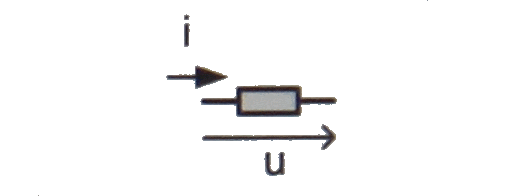
\includegraphics[width=1\linewidth]{aes_fig012a.png}      & \(u = Ri\)      \\
              \hline
              rezistor (model pro vyšší frekvence)      
                & 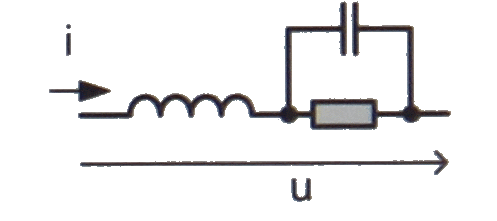
\includegraphics[width=1\linewidth]{aes_fig012b.png}      
                & náhradní schéma tvořené elementárními prvky \\ 
              \hline    
              nelineární prvek - varistor               
                & 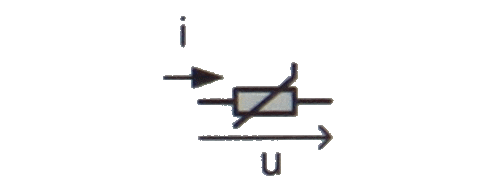
\includegraphics[width=1\linewidth]{aes_fig012c.png}      & \(i = Au^B\)    \\
              \hline
              polovodičová dioda (elementární model)    
                & 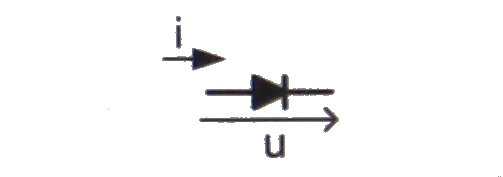
\includegraphics[width=1\linewidth]{aes_fig012d.png} 
                &  \(i = I_s\left(e^\frac{u}{nV_T}-1\right)\)  \\
              \hline 
            \end{tabular}
            \caption{Příklady modelů}\label{aes:tab001}
          \end{table*}

          Matematický model celého obvodu vznikne sloučením modelů dílčích prvků s Kirchhoffovými
          rovnicemi, které popisují interakce mezi prvky. Výsledkem je soustava tzv.
          \emph{algebraicko-diferenciálních rovnic}. Běžný uživatel simulačního programu, na rozdíl od
          jeho tvůrce, se s těmito rovnicemi přímo nesetká.

      \subsection{Simulace a realita}
        Přes všechen pokrok v oblasti počítačové podpory návrhu však dosud neexistuje program, do
        něhož by uživatel zadal obvod (schéma) a po stisknutí tlačítka obdržel důvěryhodné výsledky,
        aniž by o obvodu něco věděl. Výsledky mohou být chybné a je jen na uživateli, aby je kriticky
        posoudil. 
        
        Příčiny nesouladu mezi realitou a simulací můžeme rozdělit do čtyř kategorii:
        \begin{enumerate}[leftmargin=2cm,rightmargin=0.8cm, label=\emph{\alph*}),noitemsep]
          \item chyby vzniklé při vlastním řešení rovnic obvodového modelu v simulátoru, 
          \item nepřesné modely,
          \item výrobní rozptyl, 
          \item zanedbané parazitní prvky.
        \end{enumerate}

        \begin{itemize}[noitemsep]
          \item \textbf{Chyby simulátoru}: Při numerickém řešení soustavy rovnic, popisující obvod,
                vznikají chyby zaokrouhlováním, diskretizací i iteračním způsobem řešení.
                Pomineme-li problémy prvků popsaných ve frekvenční oblasti a tzv. špatně podmíněné
                úlohy, tak je možné říci, že přesnost výpočtu má uživatel pod kontrolou
                prostřednictvím parametrů RELTOL, ABSTOL a VNTOL (\todo[inline]{blíže v kap. 1.4.2.1}).
                Obvykle je nastavena relativní chyba \SI{0.1}{\percent}. Požadování vyšší přesnosti
                zpomalí simulaci nebo může v krajním případě vést k jejímu selhání. Je také
                diskutabilní, zdali požadovat výrazně vyšší přesnost simulace, než mohou mít měřicí
                přístroje v laboratoři. 
          \item \textbf{Nepřesné modely}: Každý model je jen aproximací reality. Používané modely
                jsou kompromisem mezi požadavkem na přesnost, výpočetní efektivitu a možnost snadné
                identifikace parametrů na základě měření.
          \item \textbf{Výrobní rozptyl}: Výrobní rozptyl je značný zejména u polovodičů. Např.
                proudový zesilovací činitel bipolárního tranzistoru může mít toleranci až
                \SI{\pm50}{\percent}.
          \item \textbf{ Odhad parazitních prvků}: Dalším problémem jsou parazitní vlastnosti
                propojovacích vodičů mezi prvky. To, co je nakresleno v editoru schématu jako vodič,
                vlastně představuje ideální spoj bez parazitní indukčnosti, odporu i kapacity.
                Zvláště při analýze obvodů v megahertzové oblasti vyžaduje odhad parazitních prvků i
                jistou zkušenost s praktickou realizací. Při neuvažování parazitních prvků vlastně
                analyzujeme neúplný model obvodu.                          
        \end{itemize}

        \begin{tcnote}
          Vliv výrobního rozptylu si ukažme na příkladu (nevhodného) nastavení pracovního body
          zesilovače v zapojení \texttt{SE}. Zapojení je velmi citlivé na parametry tranzistoru.
          Předpokládejme, že máme konkrétní kus tranzistoru \texttt{Philips/NXP BC546A}, který
          změříme a na základě změřených hodnot vytvoříme model. V tom případě bude chyba mezi
          simulací a měřením např. kolektorového proudu řádu procent.
          
          {\centering
          \captionsetup{type=figure}
            \subcaptionbox{\label{aes:fig013a}}{\luafigure[.45]{aes_fig013a.png}} 
            \hspace{1em} 
            \subcaptionbox{\label{aes:fig013b}}{\luafigure[.45]{aes_fig013b.png}}  
          \captionof{figure}{a) Nastavení pracovního bodu; b) model a skutečné prvky
                      (\cite[s.~6]{KolkaBiolek2011}) \label{aes:fig013}} \par}

        Uvažme nyní, že použijeme jiný kus téhož typu a stále stejný model. Podle údajů katalogového
        listu leží proudový zesilovací činitel \(h_{21E}(\beta)\) v rozmezí \num{110} až \num{220}.
        U druhého tranzistoru bude parametr h21e jiný, dopředu neznámý. I kdybychom vytvořili
        dokonalý model pro první tranzistor, tak při použití druhého tranzistoru dostaneme odchylku
        v řádu desítek procent.

        V praxi se navíc vytvářejí modely spíše pro typické hodnoty, které ani nemusí popisovat
        konkrétní existující kus. Na obr. \ref{aes:fig013b}  je to ilustrováno graficky (pro případ,
        kdyby měl model jen dva parametry). Je tedy zřejmé, že otázka: \uv{Jakou hodnotu bude mít
        kolektorový proud?} je nesprávně položena. Správně položená otázka zní: \uv{V jakém rozsahu
        se může nacházet kolektorový proud, když uvážíme výrobní rozptyl všech prvků?} Pak teprve
        můžeme porovnávat simulaci a realitu.

        Musíme se tedy smířit s tím, že model vždy vyjadřuje jen parametry jednoho (hypotetického)
        prvku. Dobrý model musí navíc věrně postihovat např. závislost parametrů na teplotě,
        frekvenci, nebo kolektorovém proudu.
      \end{tcnote} 

  \section{Modelování základních obvodů}
    \subsection{Typické uspořádání simulačních programů}
      Pojem \texttt{SPICE} označuje vlastní výpočetní jádro, které řeší obvodové rovnice. Moderní
      simulátory jsou obvykle součástí větších systémů pro kompletní návrh klasických nebo
      integrovaných obvodů.

      Bohužel standard \texttt{SPICE} není zaštítěn žádnou respektovanou organizací. Proto existují
      mezi jednotlivými programy drobné rozdíly v syntaxi vstupních souborů. Knihovny a vytvořené
      obvody obvykle nejsou automaticky plně přenositelné. Většinou programy zachovávají zpětnou
      kompatibilitu se syntaxí použitou ve \texttt{SPICE2} a \texttt{SPICE3}. Pokud např. výrobci
      prvků poskytují (na Internetu) modely, tak v naprosté většině právě v kompatibilní formě. To
      má za následek, že se nevyužijí možnosti, které byly přidány do různých komerčních variant
      \texttt{SPICE}.

      Na obr. \ref{aes:fig014} je ustálené uspořádání simulačního programu. Systém obvykle obsahuje
      tři moduly: \emph{editor schématu}, \emph{simulátor} a \emph{postprocesor} - modul pro
      vykreslování výsledků analýzy a jejich další zpracování. Editory schématu a postprocesory se
      od jednotlivých výrobců velmi výrazně odlišují. Z pohledu uživatele má největší význam to, že
      rozhraní editor + simulátor je víceméně standardizované. Právě tomu se říká „standard SPICE“.
      Informace o obvodu a požadovaných analýzách jsou simulátoru předávány pomocí textových
      souborů. Přenositelnost jak obvodů, tak knihoven modelů je zajištěna právě na úrovni těchto
      souborů. To je důvod, proč se všechny obvody a modely publikují jako textové soubory. Formáty
      souborů pro uložení schématu jsou většinou neveřejné, často podléhající licenci.

      \luagraphic[1]{aes_fig014.png}{Typické uspořádání simulačního programu. 
      (\cite[s.~8]{KolkaBiolek2011})}{aes:fig014}      

      Na obr. \ref{aes:fig015} je příklad organizace souborů pro stejnosměrnou analýzu jednoduchého
      obvodu s diodou, kdy napětí stejnosměrného zdroje je rozmítáno od \SI{-3}{\V} do \SI{+3}{\V}.
      Vstupní soubor je vygenerován automaticky editorem schématu nebo může být editován ručně.
      První část tvoří popis samotného obvodu. Každému prvku odpovídá jeden řádek. Parametry zdroje
      napětí (\texttt{V\_V1}) a rezistoru (\texttt{R\_R1}) jsou plně popsané v netlistu. Uzly jsou
      ve schématu očíslované jako \num{1} a \num{2}, referenční uzel je vždy \num{0}. Dioda je
      popsána složitým modelem s mnoha parametry, který je uložen v knihovně spolu s dalšími modely.
      Řádek v netlistu obsahuje jen odkaz na model.

      \luagraphic[1]{aes_fig015.png}{Struktura vstupních souborů.
      (\cite[s.~9]{KolkaBiolek2011})}{aes:fig015}      

      Jméno knihovního souboru je uvedeno v příkazu \texttt{.LIB}. V poslední části jsou příkazy pro
      rozmítání stejnosměrné složky \(V_1\) s krokem \SI{50}{\mV}. Příkaz \texttt{.PROBE} určuje, že
      napětí obou uzlů se budou ukládat pro zpracování v postprocesoru (zobrazení grafů). Model z
      knihovny (příkaz \texttt{.model...}) může být umístěný v hlavním souboru. V tom případě
      knihovnu nepotřebujeme a celá úloha je definovaná jen jedním souborem. Tento styl je výhodný,
      pokud někomu potřebujeme poskytnout náš \uv{obvod} v textové formě. Netlistem by se měl
      nazývat jen soupis prvků. Někdy se tak ovšem říká i celému vstupnímu souboru, obsahujícímu
      také příkazy.
      
      \begin{tcnote}
        Uživatel simulačního programu je prakticky vždy nucen pracovat i s textovými soubory
        knihoven nebo netlistů, například při zahrnování nového modelu do knihovny nebo hledání
        chyb podle hlášení simulátoru.
      \end{tcnote}

      Vstupní soubor z obr. \ref{aes:fig015} je možné \uv{odsimulovat} programem
      \texttt{PSpice}. Hlavní textový soubor nazveme např. jako \texttt{obvod.cir}
      a knihovnu jako \texttt{diody.lib} (text lze zkopírovat přes schránku Windows). Spustíme
      program \texttt{PSpiceAD} (nikoli editor schématu \texttt{Capture}). Zvolíme
      \texttt{File/Open} a nastavíme typ souboru na \texttt{*.cir}. Volbou \emph{Simulation/Run} se
      spustí analýza. Po skončení se pomocí \texttt{Trace/Add Trace} zobrazí např. průběh \(v(2)\) -
      napětí na diodě. \todo[inline]{Podrobnosti viz kapitola 1.2.4 na str. 20.s}

    \subsection{Základní pravidla jazyka (P)Spice}
      Kromě definice struktury obvodu a modelů prvků obsahuje vstupní soubor i příkazy pro simulátor
      k provádění různých analýz, ukládání výsledků a nastavování parametrů algoritmů pro numerické
      řešení.

      \begin{tcnote}
        Syntaktická pravidla:
        \begin{itemize}[noitemsep]
          \item První řádek vždy slouží jako hlavička (nadpis), \texttt{PSpice} jej
                ignoruje\footnote{na obr. \ref{aes:fig015} je to řádek: \texttt{* obvod}}. 
          \item Prázdné řádky, vícenásobné mezery a další „bílé znaky“ se ignorují. 
          \item Malá a velká písmena se nerozlišují. 
          \item Na pořadí řádků nezáleží (s výjimkou prvního a posledního řádku). 
          \item Názvy všech obvodových prvků musí být jedinečné. 
          \item Každý řádek (s výjimkou hlavičky) začíná jedním z těchto symbolů: 
                \begin{itemize}[noitemsep]
                  \item \textbf{znak 'A' až 'Z'} - definice obvodového prvku (např. R pro
                        rezistor\footnote{Jednotlivé verze SPICE se mohou mírně lišit v přiřazení
                        znaků k prvkům.}).
                  \item \textbf{znak '*'} - obsah řádku je chápán jako komentář. 
                  \item \textbf{znak '+'} - řádek je pokračováním předchozího řádku\footnote{Používá
                        se pro zlepšení čitelnosti.}. 
                  \item \textbf{znak '.'} - příkaz simulátoru (např. \texttt{.DC} provede
                        stejnosměrnou analýzu).
                \end{itemize}
          \item Vše, co je napravo od znaku středník ';', je chápáno jako komentář.
          \item Soubor končí příkazem \texttt{.END}. 
          \item Uzly se značí alfanumerickým řetězcem bez mezer. Původní standard dovoloval jen
                označení celými čísly. Jeden z uzlů musí být označen jako O (nula).
          \item Čísla se zapisují v přirozeném tvaru (\num{0.25}) vždy s desetinnou tečkou, v
                exponenciálním tvaru (1e-3), nebo je možné použít standardní technické přípony
                (\texttt{f, u, m, k, meg, g, t}). Mezi číslem a příponou se nesmí psát mezera.
                Ostatní znaky za číslem se ignorují (\texttt{1uF = 1u}). Přípona \texttt{m} i
                \texttt{M} znamená \texttt{mili} (\num{e-3}) - nerozlišují se malá a velká písmena. 
          \item Od \texttt{PSpice} verze 15 je možné využívat i tzv. Evropský způsob, kdy se přípona
                píše místo desetinné tečky. Např. \texttt{4k7 = 4.7k}. Místo desetinné tečky je také
                možné použít \texttt{R} pro rezistory, \texttt{L} pro induktory a \texttt{C} pro
                kapacitory. Např. \texttt{1R2 = \SI{1.2}{\ohm}}, ale jen u rezistoru.
        \end{itemize}
      \end{tcnote}

      \subsubsection{Definice prvků}
        Řádek netlistu, který definuje obvodový prvek, začíná pevně daným znakem. Jednotlivé
        varianty \texttt{SPICE} se mohou v přiřazení znaků mírně odlišovat. V programu
        \texttt{PSpice} jsou definovány tyto prvky: 

  \section{Základní analýzy}
    \subsection{Stejnosměrná analýza}
      Stejnosměrná analýza odpovídá laboratornímu experimentu, kdy např. na vstup obvodu připojíme
      regulovatelný stejnosměrný zdroj a měříme závislost výstupního stejnosměrného napětí na
      vstupním. V podstatě se jedná o sledování závislosti stejnosměrného pracovního bodu na nějaké
      veličině (napětí, proud, odpor, teplota, atd.).

      \luagraphic[1]{aes_fig019.png}{Stejnosměrná analýza.
      (\cite[s.~59]{KolkaBiolek2011})}{aes:fig019}         


      Hledání pracovního bodu si vysvětlíme na příkladu \emph{Colpittsova oscilátoru} z obr.
      \ref{aes:fig020a}. První krok spočívá v odstranění setrvačných prvků z obvodu, protože ty
      nemají na stejnosměrný pracovní bod vliv. Induktory jsou nahrazeny zkratem a kapacitory jsou
      jednoduše vypuštěny. Po odstranění setrvačných prvků zmizí z obvodových rovnic čas. Standardní
      stejnosměrná analýza proto nemůže poskytnout informaci o stabilitě či nestabilitě pracovního
      bodu. Při laboratorním měření však nelze z obvodu nikdy odstranit setrvačnost (přinejmenším ne
      parazitní prvky). Aby bylo možné měření provést, musí být u reálného systému pracovní bod
      samozřejmě stabilní. (V literatuře byly popsány metody pro odhad stability bez znalosti
      setrvačných prvků - zatím se však v praxi nepoužívají.)

      \begin{figure}[ht!]
        \centering  
        \subcaptionbox{\label{aes:fig020a}}{\luafigure[0.9]{aes_fig020a.png}}          \\
        \subcaptionbox{\label{aes:fig020b}}{\luafigure[0.5]{aes_fig020b.png}}               
        \caption{Úprava obvodu pro výpočet pracovního bodu. (\cite[s.~59]{KolkaBiolek2011})}
        \label{aes:fig020}
      \end{figure}

      Pracovní bod je charakterizován stejným napětím na kolektoru a bázi bipolárního tranzistoru,
      protože tyto svorky jsou stejnosměrně propojené přes indukčnost \(L\). Rozpojme nyní tyto
      svorky. Napětí báze je označeno jako \(U_1\), napětí kolektoru pak jako \(U_2\). Na obr.
      \ref{aes:fig021a} je znázorněna závislost \(U_2=f(U_1)\). Jedná se vlastně o zesilovač v
      zapojení \texttt{SE}. Pracovní bod se nachází tam, kde platí \(U_1 = U_2\). Na druhém grafu je
      vynesena závislost \(U_1-U_2\). V pracovním bodu tedy musí platit \(U_1 - U_2 = 0\). Hledáme
      průsečík zobrazené křivky s nulou.

      \begin{figure}[ht!]
        \centering  
        \subcaptionbox{\label{aes:fig021a}}{\luafigure[0.40]{aes_fig021a.png}}    \hspace{1em}
        \subcaptionbox{\label{aes:fig021b}}{\luafigure[0.45]{aes_fig021b.png}}               
        \caption{Princip výpočtu pracovního bodu. (\cite[s.~60]{KolkaBiolek2011})}
        \label{aes:fig021}
      \end{figure}
      
      U všech programů třídy \texttt{SPICE} je výpočet pracovního bodu prakticky shodný. Používá se
      \textbf{Newton-Raphsonova metoda tečen}. Její princip si můžeme představit podle obr.
      \ref{aes:fig021b}. Metoda hledá kořen algebraické rovnice, tj. \emph{průsečík nějaké
      funkce s osou \(x\)}. Výpočet probíhá vždy iteračně. Na počátku je nutné zvolit výchozí bod
      \(U_1^{(0)}\), ve kterém se určí tečna. Její průsečík s osou \(x\) dává nový bod (odhad
      kořene) \(U_1^{(1)}\), pak \(U_1^{(2)}\), atd.. Celý proces se iteračně opakuje. V dalších
      krocích se program blíží k průsečíku - hledanému pracovnímu bodu, který však nikdy přesně
      nedosáhne. Iterace jsou zastaveny, až chyba klesne na přijatelnou hodnotu nebo až je překročen
      maximální povolený počet iterací. V případě existence více pracovních bodů (křivka má více
      průsečíků s osou) nalezne metoda vždy jen jeden pracovní bod v závislosti na zvoleném výchozím
      bodu. Pro některé úlohy mohou iterace divergovat (vzdalují se od průsečíku). V takovém případě
      program oznámí, že pracovní bod nebyl nalezen.

      \begin{tcnote}
        Vlastnosti metody použité pro výpočet pracovního bodu je možné formulovat do následujících
        bodů:
        \begin{itemize}[noitemsep]
          \item Nalezení pracovního bodu není garantováno. Problémy se mohou vyskytnout u obvodů s
                vysokým ziskem (operační zesilovače) nebo s ostrými nelinearitami (příliš
                idealizované behaviorální modely).
          \item Čím lépe odhadneme výchozí bod, tím rychlejší a spolehlivější bude konvergence. 
          \item V případě existence více pracovních bodů najde metoda vždy jen jeden v závislosti
                na výchozím bodu. 
          \item Řešení neposkytne informaci o stabilitě nalezeného pracovního bodu.
        \end{itemize}
      \end{tcnote}

    \subsection{Analýza v časové oblasti}
      Analýza odpovídá laboratornímu experimentu, kdy obvod, na jehož vstup je připojený signální
      generátor, měříme osciloskopem. Výsledkem analýzy jsou časové průběhy napětí a proudů v
      obvodu.

      \luagraphic[1]{aes_fig016.png}{Výsledky časové analýzy.
      (\cite[s.~68]{KolkaBiolek2011})}{aes:fig016}  

      Řešení v simulátoru probíhá vždy tak, že obdržíme všechny průběhy \(u(t)\) a \(i(t)\)
      vzorkované v diskrétních časech \(t_i\), přičemž dělení časové osy není ekvidistantní.

      Časový krok si program volí automaticky podle aktuální strmosti průběhu veličin v obvodu a
      požadované přesnosti výpočtu. Při pomalých změnách se prodlužuje a při prudkých změnách
      zkracuje. Délka kroku se automaticky nastavuje tak, aby program stále počítal s přibližně
      stejnou chybou. Při pevném kroku by jeho velikost musela být nastavena podle „rychlých“ úseků.
      V úsecích s „pomalou“ změnou by malý krok zbytečně zvyšoval výpočetní náročnost, nehledě na
      akumulaci numerických chyb.

      Na obr. \ref{aes:fig017} je znázorněn algoritmus pro řízení kroku v závislosti na charakteru
      signálů. V případě pomalých změn napětí a proudů se volí velký krok. Pokud se mezi dvěma kroky
      objeví např. strmá nástupní hrana vstupního signálu, tak v čase \(t_3\) vznikne
      neakceptovatelně velká chyba (to se zjistí až po výpočtu tohoto kroku). Řešení v čase \(t_3\)
      musí být zamítnuto. Program se vrátí do \(t_2\) a pokračuje s menším krokem, např. polovičním.
      Proces zkracování kroku pokračuje tak dlouho, dokud se nedosáhne akceptovatelné chyby. Naopak
      pokud řešení probíhá s chybou menší než je povolená hodnota, tak se krok prodlužuje.

      
      \luagraphic[1]{aes_fig017.png}{Princip automatické volby časového kroku.
      (\cite[s.~68]{KolkaBiolek2011})}{aes:fig017}  

      Dynamická změna kroku má ovšem své meze. Shora je krok omezen délkou intervalu, na kterém
      probíhá řešení tak, aby výsledkem byl „rozumný“ počet bodů, ze kterého je možné sestavit graf
      (např. \num{50} až \num{100} hodnot). Zdola je krok omezen přesností zobrazení čísel v
      počítači. Předpokládejme, že je čas v simulátoru reprezentován proměnnou typu double s
      přesností \num{15} míst. Pokud by např. došlo ke zkrácení kroku z důvodu velmi strmé hrany na
      \(\Delta t = \num{e-20}\) v čase \(t = \SI{1}{\second}\), tak nový časový okamžik bude opět
      \(\num{1} + \num{e-20} \approx 1\), protože je čas reprezentován omezeným počtem míst. Výpočet
      by se proto zastavil. Pro krok je možné formulovat podmínku

      \begin{equation}\label{aes:eq024}
        \frac{T_{max}10^{-m}}{tol} \leq h \leq \frac{T_{max}}{N}, 
      \end{equation}

      kde \(T_{max}\) je délka simulačního simulačního intervalu. \(N\) bývá v rozsahu \num{50} až
      \num{100}, \(m\) je počet platných míst (\num{15} pro \emph{double} a \(tol\) je povolená
      relativní chyba zobrazení času (např. \num{e-3}).

      Není-li možné dodržet předepsanou chybu výpočtu při splnění podmínky (\ref{aes:eq024}), tak je
      řešení ukončeno. Potom je nutné provést změny v samotném obvodu, nastavení analýzy nebo
      globálních podmínek simulátoru. Následující odstavec uvádí některá doporučení, založená na
      praktických zkušenostech uživatelů:

      \begin{tcnote}
        \begin{itemize}[noitemsep]
          \item Používat spojité a hladké funkce při vytváření modelů. Doplnit nelinearitu o
                parazitní kapacitu (paralelně ke zdroji proudu) či indukčnost (sériově ke zdroji
                napětí).
          \item Zmenšit délku simulačního intervalu, snížit požadavek na přesnost. 
          \item Nepoužívat ideální impulzní signály (s nulovou délkou hrany). Např. ideální
                jednotkový skok není stejně možné v praxi realizovat. Nastavíme-li délku hrany o
                \num{4} řády kratší než je nejmenší časová konstanta v obvodu (stačí odhad), tak
                dostaneme číselně stejný výsledek jako pro ideální signál.
        \end{itemize}
      \end{tcnote}

      \subsection{Stabilita integrační metody}
        Při numerickém řešení v časové oblasti se \emph{soustava algebraicko-diferenciálních rovnic}
        (spojitý čas) matematického modelu obvodu převádí na \emph{soustavu diferenčních rovnic}
        (diskrétní čas). Při tomto převodu nastávají problémy se \textbf{stabilitou}. Je přirozené, že
        při analýze stabilního obvodu potřebujeme, aby simulovaná odezva byla také stabilní a výsledky
        tak odpovídaly realitě. Tento požadavek však není splněn automaticky mimo jiné proto, že
        závisí na typu řešené úlohy. Aby bylo možné srovnávat jednotlivé metody, používá se standardně
        testovací diferenciální rovnice prvního řádu ve tvaru
        \begin{equation}\label{aes:eq025}
          \dot{x} = \lambda x, 
        \end{equation}
        kde \(\lambda\) je komplexní kořen charakteristické rovnice (v případě přenosu by to byl
        pól). Přesné řešení rovnice je ve tvaru \(x(t) = C\exp(\lambda t)\). Rovnovážný stav \(x =
        0\) je stabilní, pokud \(\realset(\lambda)\leq0\). Stabilita numerického řešení se
        vyhodnocuje zobrazením součinu \(\Delta t\lambda\) (\(\Delta\) je \emph{časový krok}) do
        komplexní roviny. Protože časový krok je vždy kladný, \(\Delta t>0\), tak bychom u ideální
        metody čekali, že bude poskytovat stabilní \emph{numerické} řešení pro všechna
        \(\Delta t\lambda\) ležící v levé polorovině, viz obr. \ref{aes:fig018a}. Tuto vlastnost
        splňuje pouze tzv. \textbf{lichoběžníková metoda}, u které se však projevují parazitní
        zákmity při analýze impulzních obvodů. Z toho důvodu se více používají metody, které tuto
        vlastnost nemají.

        \begin{figure}[ht!]
          \centering  
            \subcaptionbox{\label{aes:fig018a}}{\luafigure[0.45]{aes_fig018a.png}}  \hspace{1em}            
            \subcaptionbox{\label{aes:fig018b}}{\luafigure[0.45]{aes_fig018b.png}}  \\            
            \subcaptionbox{\label{aes:fig018c}}{\luafigure[0.45]{aes_fig018c.png}}  
          \caption{Oblast absolutní stability a) lichoběžníková metoda; b), c) Gearova metoda}
          \label{aes:fig018}
        \end{figure}

        Jedna z nejrozšířenějších metod, která je využita i v \texttt{PSpice}, je tzv.
        \textbf{Gearova metoda}. Na obr. \ref{aes:fig018b} a \ref{aes:fig018c} jsou
        vyznačené oblasti její stability. Řád metody (tj. stupeň polynomu, který lokálně aproximuje
        řešení) se automaticky mění podobným způsobem jako časový krok. Při zkracování kroku se
        používá nižší řád a naopak.

        Pro řád \num{2} vidíme, že metoda poskytuje stabilní řešení i v případě, že kořen (pól) leží
        v pravé polorovině! Naopak pro řád \num{5} poskytuje nestabilní řešení i v případě, že kořen
        (pól) leží v levé části komplexní poloroviny. Tím se stává problematickým použití časové
        simulace pro odhalení nestability, zvláště v případech, kdy kořeny (póly) leží blízko
        imaginární osy.

        \subsection{Střídavá analýza}

        \luagraphic[1]{aes_fig022.png}{Výsledky střídavé analýzy - modulová charakteristika v
        \si{\decibel}. (\cite[s.~79]{KolkaBiolek2011})}{aes:fig022}  

        \luagraphic[1]{aes_fig023.png}{Výpočet střídavé odezvy integračního článku.
        (\cite[s.~79]{KolkaBiolek2011})}{aes:fig023}  

        
  \section{Simulace a analýza v programu LTspice IV}
   
  \section{Příkazy pro řízení simulace}
    
    \begin{figure}[ht!]
      \centering
      \subcaptionbox{\label{SPICE:fig_ltc001_Ra}}{\luafigure[0.45]{../ltspice/ltc001_RC.pdf}}
      \subcaptionbox{\label{SPICE:fig_ltc001_Rb}}{\luafigure[0.45]{../ltspice/CompAttrEditor.png}}  
      \caption{\texttt{ltc001\_RC.asc}: Nastavení počáteční velikosti napětí na které je 
               kondenzátor nabit}
      \label{SPICE:fig_ltc001}
    \end{figure}

  \section{Úvod do simulace spínaných napájecích zdrojů}
    % In the electronics world, different types of circuitries must cohabit: logic devices, analog 
    % circuits, microprocessors, and so on. Unfortunately for the designer, these circuits do not 
    % cope with a single, fixed, power supply rail: A microprocessor or a digital signal processor 
    % (DSP) will need a stable 3.3-V source or less, a front-end acquisition board will require ±15 
    % V and perhaps some logic glue around a standard 5 V. For the final board being supplied from 
    %%% a single power point, for example, the mains outlet or a battery, how is one to adapt and 
    % distribute all these different voltages to the appropriate portions? The solution consists of 
    % inserting a so-called converter to adapt the voltage distribution to the circuit needs.
    
    Ve světě elektroniky (obr. \ref{SPICE:Basso_intro}), musí různé druhy elektronických obvodů 
    vzájemně spolupracovat (logické obvody, analogové obvody, mikroprocesory, atd.). Bohužel tyto 
    obvody nepracují s jediným napájecím napětím: mikroprocesor nebo signálový procesor (DSP), bude 
    potřebovat například zdroj \SI{3.3}{\volt}, analogové obvody mohou vyžadovat symetrické nápení 
    \SI{\pm15}{\volt}. Ovšem externí napájecí zdroj je zpravidla jen jeden (např. síťové napájení 
    \SI{230}{\volt}, baterie). Vzniká tak otázka, jakým způsobem z tohoto zdroje realizovat tolik 
    napájecích úrovní. Řešení spočívá ve vložení tzv. převodníku mezi zdroj a napájený obvod, který 
    přizpůsobí napájecí napětí konkrétním požadavkům obvodu.
    
    \begin{figure}[ht!]
      \centering
      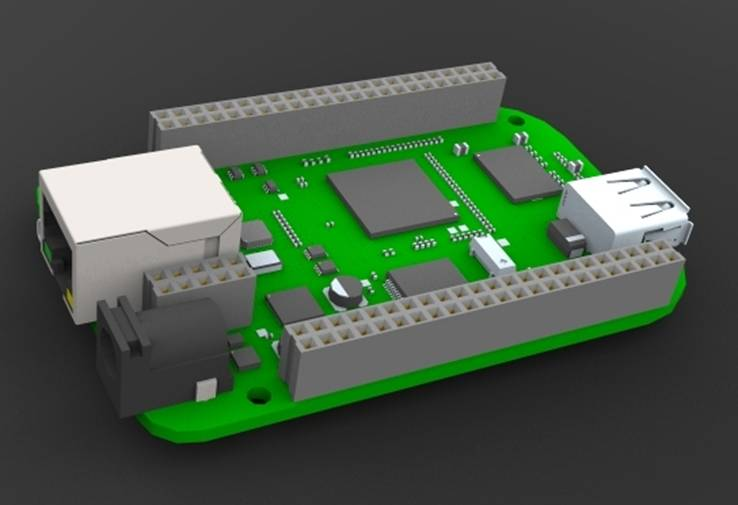
\includegraphics[width=0.6\linewidth]{beaglebone.jpg}
      \caption{Příklad plošného spoje s mnoha druhy integrovaných obvodů, vyžadující odlišné 
               napájecí úrovně}
      \label{SPICE:Basso_intro}
    \end{figure}

%---------------------------------------------------------------------------------------------------
  % % !TeX spellcheck = cs_CZ
{\tikzset{external/prefix={tikz/AES/}}
 \tikzset{external/figure name/.add={ch02_}{}}
%---------------------------------------------------------------------------------------------------
% file amplifier.tex
%---------------------------------------------------------------------------------------------------
%============================ Kapitola: Zesilovače==================================================
\chapter{Zesilovače}
\minitoc

  V této kapitole se budeme zabývat rozbory vlastností základních obvodů a jejich účelným
  spojováním do funkčních bloků určených pro zesilování signálů. \cite[p.~101]{Neumann}
  
  \section{Zjednodušení výpočet tranzistorového ze\-si\-lo\-va\-če}
    Přesný výpočet tranzistorového zesilovače vychází z určení dvojbranových pa\-ra\-me\-trů
    tranzistoru a pokračuje sestavením matice obvodu a řešením této matice. Při použití vybraných
    rovnic matematických modelů pro programy SPICE lze dojít ke zjednodušenému řešení, ve kterém se
    některé parametry zanedbají a sestavené náhradní schema pak řešit libovolnou metodou. Přesto
    dostaneme výsledky s přesností, která pro obvyklé technické řešení postačuje.

    \subsection{Obecná převodní charakteristika bipolární tranzistoru}
      Převodní charakteristika udává závislost výstupního proudu na vstupním napětí. Pro zapojení
      \texttt{SE} představuje převodní charakteristiku exponenciální závislost kolektorového proudu
      na napětí mezi bází a emitorem. Strmost je dána derivací funkce (tečnou) v daném pracovním
      bodě a odpovídá parametru $\mathrm{y_{21}}$.

} % tikzset
%---------------------------------------------------------------------------------------------------
\printbibliography[title={Seznam literatury}, heading=subbibliography]
\addcontentsline{toc}{section}{Seznam literatury}

  % % !TeX spellcheck = cs_CZ
%---------------------------------------------------------------------------------------------------
% file oscillator.tex
%---------------------------------------------------------------------------------------------------
%======================== Kapitola: Generátory signálů==============================================
\setchaptertoc
\chapter{Generátory signálů}


  \textbf{Generátory signálů} jsou elektronické obvody, které za určitých podmínek generují 
  jednorázový nebo periodický signál. Na rozdíl od zesilovačů nejsou buzeny z vnějších zdrojů 
  signálů, patří tedy mezi \emph{autonomní obvody}.
  
  \begin{itemize}[noitemsep]
    \item \emph{Podle druhu vyráběných signálů:}
      \begin{itemize}
        \item neperiodických průběhů (jednorázových)
        \item periodických průběhů.
      \end{itemize}
    \item  \emph{Podle tvaru generovaného signálů:}
    \begin{itemize}
      \item harmonických signálů - \emph{oscilátory}
      \item impulzních průběhů - \emph{klopné obvody}
      \item funkční generátory - vytvářejí různé periodické průběhy jako trojúhelníkové, pilovité, 
            můžeme sem zařadit také generátory speciálních průběhů, jako jsou generátory, televizního signálů
            apod.
    \end{itemize} 
  \end{itemize}
  
  Mezi hlavní vlastnosti generátorů zahrnujeme tyto parametry:
  \begin{itemize}[noitemsep]
    \item kmitočet (perioda) kmitů
    \item stabilita kmitočtu a amplitudy
    \item doba náběžné a sestupné hrany impulzů - v \emph{klopných obvodech} 
    \item zkreslení harmonického průběhu - u \emph{oscilátorů}.
  \end{itemize}

  \section{Generátory harmonických signálů - oscilátory}
    Základními typy oscilátorů jsou:
    \begin{itemize}[noitemsep]
      \item Jednobranové LC oscilátory, též nazývané oscilátory se záporným diferenciálním odporem 
            (\emph{Negative Resistance Oscillators});
      \item Zpětnovazební oscilátory;
      \item Oscilátory RC;
      \item LC oscilátory;
      \item Krystalem řízené oscilátory.
    \end{itemize}

    Pro pásmo nízkých kmitočtů do několika set kHz může být sinusový signál generován oscilátorem s 
    RC selektivním zpětnovazebním obvodem, pro vyšší kmitočty jsou používány LC oscilátory. Pro 
    velmi přesné a stabilní oscilátory jsou využívány oscilátory řízené krystaly.
    
    \subsection{LC oscilátory se záporným diferenciálním odporem}
      Připojíme-li k paralelnímu rezonančnímu LC obvodu zdroj proudu o proměnném kmitočtu podle 
      obr. \ref{AES:fig_MUE6_311b}, na kterém jsou sériové ztrátové odpory přepočítány na paralelní 
      vodivost \(G_p\), můžeme získat modulové charakteristiky podle obr. \ref{AES:fig_MUE6_311a}. 
      Kmitočtová závislost přenosu je závislá na velikosti činitele jakosti obvodu \(Q\) (na 
      velikosti činných ztrát v obvodu). Čím užší je rezonanční křivka a stabilnější kmitočet 
      \(\omega_0\), tím přesnější a stabilnější je kmitočet oscilátoru.

      \begin{figure}[ht!]
        \centering     
        \subcaptionbox{\label{AES:fig_MUE6_311a}}{\luafigure[0.5]{MUE6_311a.pdf}} 
        \subcaptionbox{\label{AES:fig_MUE6_311b}}{\luafigure[0.4]{MUE6_311b.png}}  \\
        \subcaptionbox{\label{AES:fig_MUE6_311c}}{\luafigure[0.4]{MUE6_311c.png}} 
        \subcaptionbox{\label{AES:fig_MUE6_311d}}{\luafigure[0.5]{MUE6_311d.pdf}}  \\
        \subcaptionbox{\label{AES:fig_MUE6_311e}}{\luafigure[0.5]{MUE6_311e.pdf}} 
        \caption{a) Modulové charakteristiky paralelního rezonančního obvodu pro napěťový přenos.
                 b) model paralelního rezonančního obvodu a jeho napájení ze zdroje o proměnném 
                 kmitočtu, c) přeměna rezonančního obvodu v oscilátor, d) časová závislost napětí 
                 na svorkách ztrátového LC obvodu po rozkmitání, d) výstupní napětí bezeztrátového 
                 LC obvodu 
                 \cite[s.~135]{Dolecek2009}.}
        \label{AES:fig_MUE6_311}
      \end{figure}
      
      Na obr. \ref{AES:fig_MUE6_311c} je nakreslen paralelní rezonanční obvod, u kterého do obvodu 
      po přepnutí spínače z polohy \(1\) do polohy \(2\) připojujeme předem nabitý kondenzátor. V 
      obvodu vzniknou vlastní tlumené kmity o kmitočtu \(\omega_0\). Obvod lze popsat diferenciální 
      rovnicí
      \begin{equation}\label{AES:eq_osc04}
        \dder{i}{t} + \frac{R}{L}\cdot\der{i}{t} + \omega^2 i = 0
      \end{equation}
      Rovnice má řešení
      \begin{equation}
        i(t) = I_{0}e^{-\delta t}\sin\omega_v t  \qquad u(t) = U_{0}e^{-\delta t}\cos\omega_v t
      \end{equation}
      kde \(I_0\) je \emph{počáteční amplituda proudu}, \(U_0\) je \emph{počáteční amplituda napětí 
      na kapacitoru}, \(\delta = \frac{R}{2L}\) je \textbf{činitel tlumeni obvodu}, \(\omega_0 
      =\frac{1}{\sqrt{LC}}\) je \textbf{rezonanční kmitočet} a \(\omega_v = \sqrt{\omega^2_0 - 
      \delta^2}\) je \textbf{vlastní kmitočet volných kmitů} obvodu. 
      
      Ze vztahu (\ref{AES:eq_osc04}) je zřejmé, Že je-li činitel tlumeni a \textbf{kladný} je 
      kmitání \textbf{tlumené}, je-li a \textbf{záporný} je kmitání \textbf{netlumené}, je-li 
      \(\delta = 0\) mají kmity konstantní amplitudu. Velikost činitele tlumení je závislá na 
      velikosti rezistoru \(R\), který modeluje ztráty v rezonančním obvodu viz obr. 
      \ref{AES:fig_MUE6_311d}, \ref{AES:fig_MUE6_311e}.
      
      V reálném obvodu je vždy \(\delta > 0\) a proto pozorujeme tlumené kmity, jejichž amplituda 
      klesá exponenciálně podle vztahu 
      \begin{equation}\label{AES:eq_osc02}
        u(t) = U_{ss}e^{-\delta t},
      \end{equation}
      kde \(u(t)\) představuje časovou závislost amplitudy kmitů na svorkách paralelního LC obvodu. 
      Dosáhnout nulového tlumení je možné sériovým zapojením rezistoru \(-R_N = R\) - tedy 
      rezistoru se \textbf{záporným odporem}. K tomu by bylo zapotřebí najít takovou součástku, 
      jejíž voltampérová charakteristika vykazuje úsek se zápornou derivací. Hledáme tedy součástky 
      které mají voltampérovou charakteristiku jako je na obr. \ref{AES:fig_AES62a} nebo 
      \ref{AES:fig_AES62b}.
      
      \begin{figure}[ht!]
        \centering  
        \subcaptionbox{nelinearita typu \textbf{S} \label{AES:fig_AES62a}}{\luafigure[0.5]{AES_62a.pdf}}
        \subcaptionbox{nelinearita typu \textbf{N} \label{AES:fig_AES62b}}{\luafigure[0.5]{AES_62b.pdf}}                                          
        \caption{Voltampérové charakteristiky s úseky vykazující záporný diferenciální odpor 
        \cite[s.~93]{Koucky1997}}
        \label{MIT:fig_AES_62}
      \end{figure}
      
      Pro sériový model kmitavého obvodu obr. \ref{AES:fig_AES63a} je použitelná nelinearita 
      \texttt{typu S} (např. lavinová dioda), pro paralelní model kmitavého obvodu obr. 
      \ref{AES:fig_AES63b} je použitelná nelinearita \texttt{typu N} (např. tunelová dioda) 
      \cite[s.~93]{Koucky1997}.

      \begin{figure}[ht!]
        \centering  
        \subcaptionbox{sériový rezonanční obvod   \label{AES:fig_AES63a}}{\luafigure[0.5]{AES_63a.pdf}} 
        \subcaptionbox{paralelní rezonanční obvod \label{AES:fig_AES63b}}{\luafigure[0.5]{AES_63b.pdf}}                                           
        \caption{ }
        \label{MIT:fig_AES_63}
      \end{figure}
      
      Na velikosti ztrátového odporu \(R\) závisí velikost činitele tlumení \emph{(damping factor)} 
      obvodu podle vztahu:
      \begin{equation}\label{AES:eq_osc01}
        \delta = \frac{R}{2L} \qquad [rad/s]
      \end{equation}
      
      LC oscilátory obsahují klasický rezonanční obvod, jehož rezonanční kmitočet je určen 
      \textbf{Thomsonovým vztahem}:
      \begin{equation}\label{AES:eq_osc03}
        f_0 = \frac{1}{2\pi\cdot\sqrt{LC}} \quad [Hz], \;\text{nebo}\; 
        \omega_0 = \frac{1}{\sqrt{LC}} \quad [rad/s].
      \end{equation}
      
%---------------------------------------------------------------------------------------------------
  % % !TeX spellcheck = cs_CZ
{\tikzset{external/prefix={tikz/AES/}}
 \tikzset{external/figure name/.add={ch05_}{}}
%---------------------------------------------------------------------------------------------------
% file DA_AD_converter.tex
%---------------------------------------------------------------------------------------------------
%======================= Kapitola: Konverze mezi digitálním a analogový signálem====================
\chapter{Konverze mezi digitálním a analogový sig\-ná\-lem}
\minitoc

\section{Konverze mezi digitálním a analogový signálem}
  Při zpracování analogového signálu je jednou z důležitých funkcí převod tohoto signálu z analogové podoby do číslicové a naopak. Proto jsou analogově-číslicové převodníky resp. číslicově-analogové převodníky (ADC - Analog-to-Digital Converter), (DAC - Digital-to-Analog Converter) velmi důležitými prvky jakéhokoli systému zpracovávajícího signál \cite[s.~11]{Haze}. Na obrázku \ref{AES:fig_ADC_DAC_IO} je definováno rozhraní obou typů převodníku.
  \begin{figure}[ht!]
     \centering
     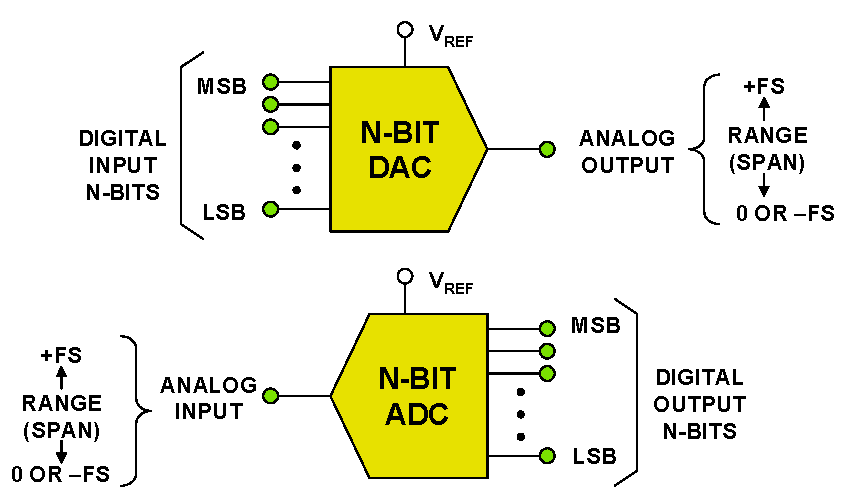
\includegraphics[width=\linewidth]{ADC_DAC_block.pdf}
     \caption[Definice I/O bloku DAC a ADC ]{Definice rozhraní bloku analogově-číslicového (ADC) a číslicově-analogového (DAC) převodníku}
     \label{AES:fig_ADC_DAC_IO}
  \end{figure}

  \textbf{Analogově-číslicové převodníky} (Analog-to-Digital Converters) slouží k pře\-ve\-de\-ní 
  analogového signálu na signál číslicový. Pro A/D převodník má analogová stupnice vstupního 
  signálu délku \texttt{FS} (\emph{Full scale}), udávanou např. ve voltech. Stupnice číslicového 
  signálu pak vyznačuje diskrétní hodnoty výstupu, které převodník generuje při převodu analogového 
  signálu \cite[s.~202]{Neumann}.

  \textbf{Číslicově-analogové převodníky} (Digital-to-Analog Converters) slouží k o\-pač\-né\-mu 
  procesu, tedy k pře\-ve\-de\-ní číslicového signálu na signál analogový, což by šlo realizovat 
  pomocí lineárního digitálního potenciometru a připojeného zdroje referenčního napětí na jeho 
  vstupu \cite[s.~208]{Neumann}. Pro N-bitové binární slovo by musel mít $n-1$ rezistorů a $n$ 
  resp. $2n - 1$ spínačů. To je monoliticky téměř nerealizovatelné již pro osmi- a vícebitové 
  slovo. Řešení převodníků proto musí být mnohem úspornější, i když úspory budou vykoupeny jinými 
  nevýhodami, případně omezeními pro jejich použití.

    \subsection{Základní struktura převodníků}
      Obě skupiny převodníků mohou typicky obsahovat komparátory, číslicové obvody, spínače, 
      integrátory, vzorkovací obvody a/nebo pasivní součástky. Nezbytnou a důležitou součástí je i 
      přesný zdroj referenčního napětí. V mnoha případech pak také platí, že DAC je jednou z částí 
      ADC.
      
      Analogově číslicový převod můžeme pomyslně rozložit do tří etap \cite{Sebesta}.
      \begin{enumerate}\addtolength{\itemsep}{-0.5\baselineskip}
        \item Převod signálu se spojitým časem na signál s diskrétním časem. Tomuto převodu říkáme  
              vzorkování.
        \item Kvantování vzorku s cílem vyjádřit vzorky konečnou množinou čísel. Tento krok je 
              provázen vznikem tzv. kvantovacího šumu. Uvedený jev souvisí s nelineárním zkreslením 
              známým z teorie obvodů.
        \item Kódování spočívající zpravidla v binárním vyjádření čísel představujících velikosti  
              vzorku.
      \end{enumerate}
      
    \subsection{Statické a dynamické parametry převodníků}
      Statické parametry převodníků jsou určovány pomocí \emph{převodní charakteristiky}, zatím co dynamické vlastnosti se vyhodnocují z kmitočtového spektra převodníku \cite[s.~11]{Haze}.
      \begin{itemize}\addtolength{\itemsep}{-0.5\baselineskip}
        \item rozsah,
        \item integrální a diferenciální nelinearita (\emph{integral - INL, differential - DNL nonlinearity}),
        \item rozlišení převodníku (\emph{resolution}),
        \item přesnost (\emph{accuracy}),
        \item chyba monotónnosti,
        \item chyba nastavení nuly (\emph{offset error}),
        \item hystereze a další.
       \end{itemize}
       K hlavním dynamickým parametrům patří
       \begin{itemize}\addtolength{\itemsep}{-0.5\baselineskip}
         \item odstup signál - šum (\emph{signal to noise ratio - SNR}) kap. \ref{AES:cap_SNR},
         \item efektivní počet bitů (\emph{effective number of bits - ENOB}),
         \item harmonické zkreslení (\emph{total harmonic distortion - THD}),
         \item odstup signál-šum a zkreslení (\emph{signal to noise and distortion - SINAD}),
         \item dynamický rozsah bez parazitních složek \newline(\emph{spurious free dynamic range 
               - SFDR}),
         \item šum - vrcholový, efektivní (\emph{noise - peak, rms}),
         \item doba přepnutí a ustálení.
       \end{itemize}

    \subsection{Vzorkování}
    \subsection{Kvantování}
       Pro přechod od časově spojitého signálu se spojitou množinou hodnot k číslicovému signálu, 
       je nutné provést (výškové) \texttt{kvantování}, tj. kvantování hodnot signálu, které je 
       patrné z obrázku \ref{AES:fig_Quntized_sig_wave}. Je zřejmé, že mapování spojitého intervalu 
       vstupních hodnot na diskrétní hodnoty digitálního výstupu způsobí, že každá hodnota 
       digitálního výstupu platí pro vstupní signál měnící se v určitém  podintervalu. Délka 
       podintervalu, pro který platí jedna hodnota digitálního výstupu se nazývá 
       \textbf{kvantizační krok převodníku} - \emph{Q}, jenž je roven bitu s nejnižší váhou - 
       \texttt{LSB}.

       \begin{figure}[ht!]
         \centering
         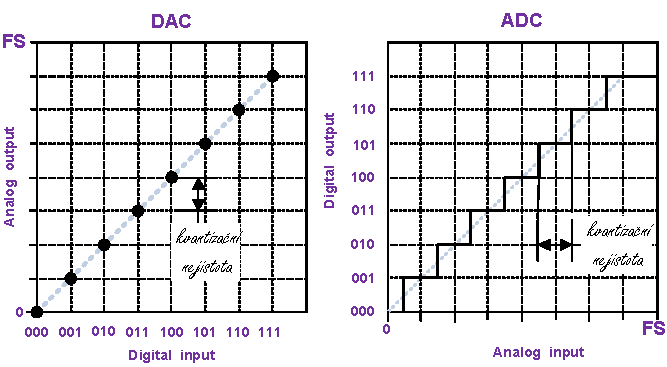
\includegraphics[width=1\linewidth]{ADC_DAC_3bit.pdf}
         \caption[Přenosová funkce AD a DA převodníku]{Ideální přenosová funkce 3bitového    
                  unipolárního AD a DA převodníku. V případě DA převodníku je přenosová funkce 
                  tvořena osmi body, nikoliv čárou.}
         \label{AES:fig_3b_DAC_ADC}
       \end{figure}
 
       Převodní charakteristika DA i AD převodníku je znázorněna na obr. \ref{AES:fig_3b_DAC_ADC}. 
       Analogový signál je spojitý a číslicový signál vyjadřuje jen jeho vybrané diskrétní hodnoty. 
       Proto je převodní charakteristika nespojitá. Naproti tomu digitální vstup vytvoří na výstupu 
       pouze omezený počet hodnot výstupního signálu.

       \begin{figure}[ht!]
         \centering
         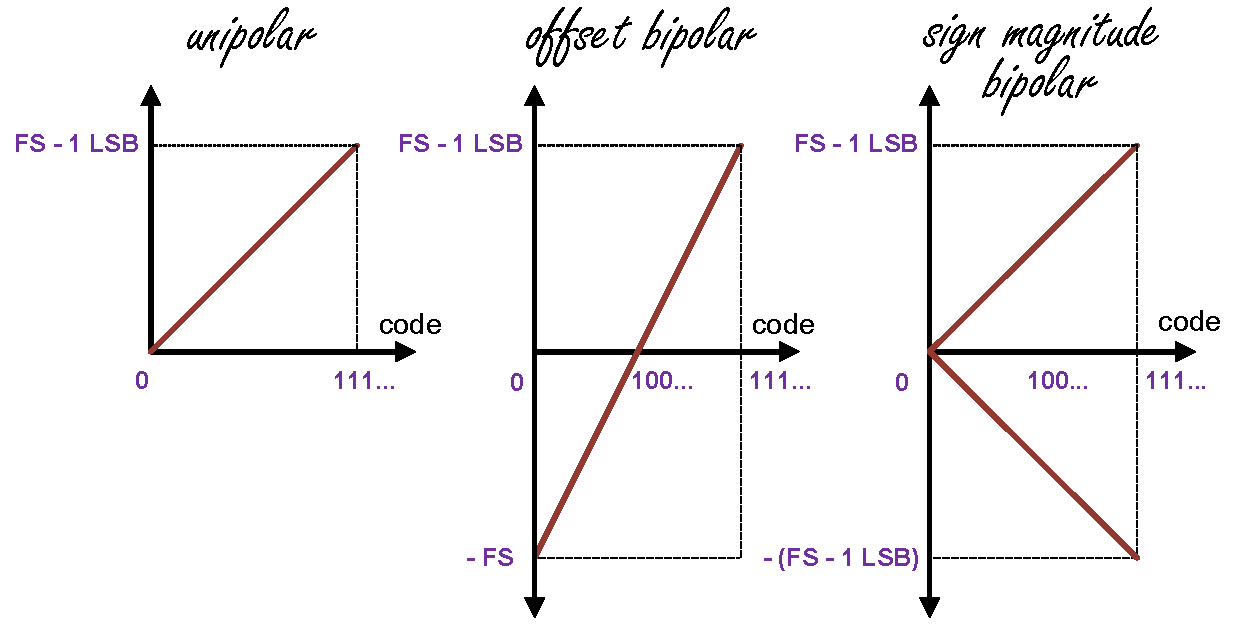
\includegraphics[width=1\linewidth]{Uni_Bi_Converter.pdf}
         \caption[Unipolární a bipolární převodníky]{Unipolární a bipolární převodníky \cite{Kester2004}}
         \label{AES:fig_uni_bi_converter}
       \end{figure}

       Počet úrovní AD převodníku, do kterého je rozdělen rozsah vstupního analogového signálu 
       definuje \textbf{rozlišovací schopnost ADC} a lze ji vyjádřit různými způsoby, jak ukazuje 
       tabulka \ref{AES:tab_10b_ADC_resolution} pro 2 až 24bitového převodníku.

         \begin{table*}[ht!]
           \centering
            \setlength{\tabcolsep}{5pt}
            \begin{tabular}{|c|c|c|c|c|c|}
              \hline
                \textbf{Rozlišení} & \multirow{2}{*}{$\mathbf{2^N}$} &  \textbf{Napětí} & 
                \multirow{2}{*}{\textbf{ppm FS}}& \multirow{2}{*}{\textbf{\% FS}}&   
                \multirow{2}{*}{\textbf{dB FS}}                                                 \\
                         N     &           &  \textbf{10V FS} &        &             &          \\
              \hline
                       2-bit   &         4 &            2.5 V & 250000 &          25 &  -12     \\
              \hline
                       4-bit   &        16 &           625 mV &  62500 &        6,25 &  -24     \\
              \hline
                       6-bit   &        64 &           156 mV &  15625 &        1,56 &  -36     \\
              \hline
                       8-bit   &       256 &          39,1 mV &   3906 &        0,39 &  -48     \\
              \hline
                      10-bit   &      1024 &          9,77 mV &    977 &       0,098 &  -60     \\
              \hline
                      12-bit   &      4096 &          2.44 mV &    244 &       0,024 &  -72     \\
              \hline
                      14-bit   &     16384 &       610 $\mu$V &     61 &       0,061 &  -84     \\
              \hline
                      16-bit   &     65536 &       153 $\mu$V &     15 &      0,0015 &  -96     \\
              \hline
                      18-bit   &    262144 &         38 $\mu$ &      4 &      0,0004 & -108     \\
              \hline
                      20-bit   &   1048576 &       9.54 $\mu$ &      1 &      0,0001 & -120     \\
              \hline
                      22-bit   &   4194304 &       2.38 $\mu$ &   0,24 &    0,000024 & -132     \\
              \hline
                      24-bit   &  16777216 &           596 nV &   0,06 &    0,000006 & -144     \\
              \hline
           \end{tabular}
           \caption[Kvantizace: Velikost LSB]{Porovnání rozlišovací schopnosti AD převodníku s  
                    různou délkou výstupního slova. Z tabulky vyplývá, že kvantizační krok 
                    24bitového ADC odpovídá velikosti úbytku na rezistoru $2,2 k\Omega$ při teplotě 
                    25°C, který vzniká vlivem tepelného šumu (viz Johnsonův šum) jenž je při šířce 
                    pásma 10 kHz roven 600 nV. }
           \label{AES:tab_10b_ADC_resolution}
         \end{table*}

       \begin{figure}[ht!]
         \centering
         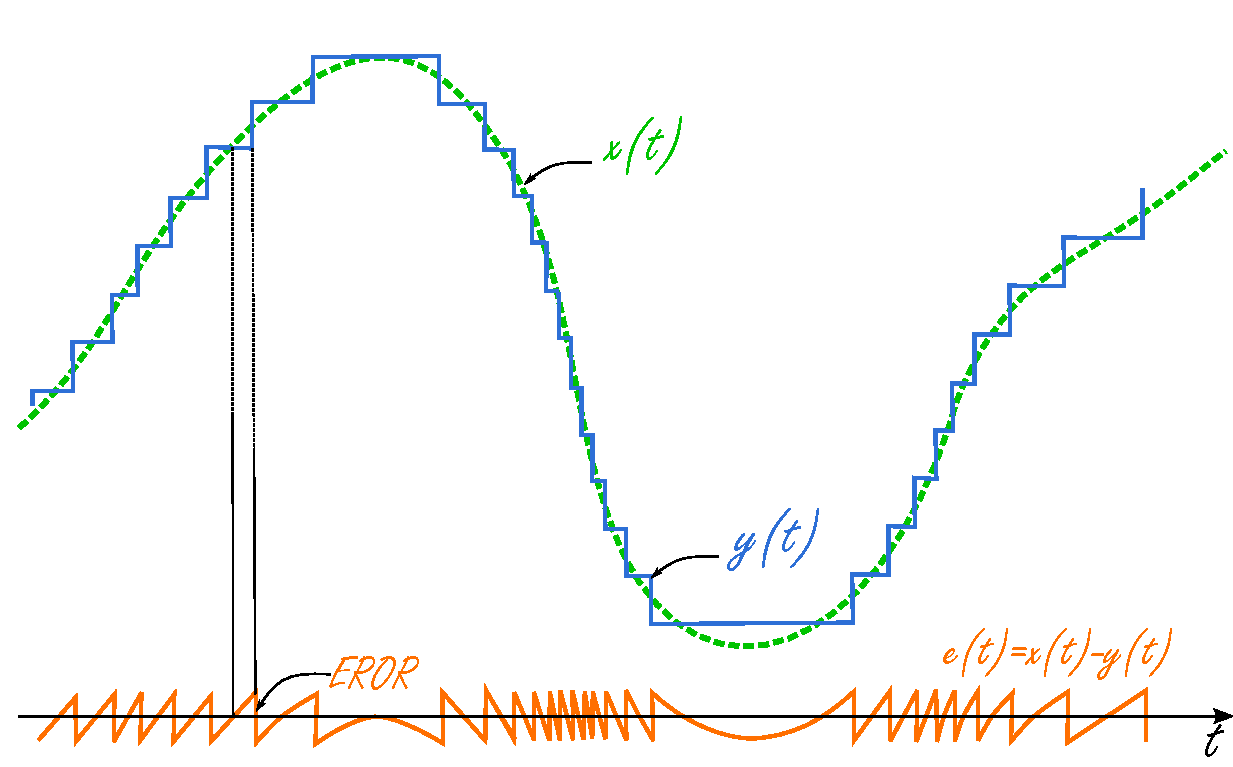
\includegraphics[width=1\linewidth]{Quantized_signal_wave.pdf}
         \caption[Kvantizační chyba]{Kvantizační chyba je rovna rozdílu původního x(t) a kvantovaného signálu v úrovni y(t) \cite{Bennett}}
         \label{AES:fig_Quntized_sig_wave}
       \end{figure}

       %The quantization error for any ac signal which spans more than a few LSBs can be 
       %approximated by an uncorrelated sawtooth waveform having a peak-to-peak amplitude of q, the 
       %weight of an LSB. Although this analysis is not precise, it is accurate enough for 
       %most applications. W. R. Bennett of Bell Laboratories analyzed the actual spectrum of 
       %quantization noise in his classic 1948

       Kvantizační chyba, jejíž průběh je na obr. \ref{AES:fig_Quntized_sig_wave}, v dynamickém 
       režimu, tj. při časových změnách vstupní analogové veličiny, způsobuje \textbf{kvantizační 
       šum}. Ten lze pozorovat např. tehdy, kdy čísla získaná z převodníku A/D jsou vedena do 
       převodníku D/A a jím je analogový signál rekonstruován. Rekonstruovaný signál se jeví jako 
       signál původní, avšak se superponovaným rušivým signálem. Vzájemným odečtení 
       rekonstruovaného a původního signálu, dostaneme samostatný rušivý signál, který lze podrobit 
       analýze. \emph{Pokud je vzorkovací signál nekorelovaný se vzorkovaným signálem, je možno 
       kvantizační šum považovat za náhodný}. Vztah mezi původním signálem a signálem degradovaným 
       kvantizačním šumem vyjadřuje parametr - \texttt{SNR}
       \begin{itemize}
         \item SNR  - Signal to Noise Ratio: poměr signálu k šumu
             \begin{equation}\label{AES:eq_SNR}
                SNR = \frac{E\{x^2(t)\}}{E\{[y(t)-x(t)]^2\}}
             \end{equation}
                \begin{itemize}
                   \item $E\{.\} \cdots$ operátor průměrování
                   \item $x(t)   \cdots$ vstupní analogový signál
                   \item $y(t)   \cdots$ rekonstruovaný kvantovaný signál
                 \end{itemize}
       \end{itemize}
       Kvantizační chybu lze aproximovat nekorelovaným pilovým průběhem s amplitudou špička-špička 
       rovnou kvantizačnímu kroku $Q$. Ačkoliv takto provedená analýza (viz kapitola 
       \ref{AES:kap_kv_sum}) není přesná, v běžných aplikacích zcela postačuje.

       Na obr. \ref{AES:fig_AD_kvantizacni_chyba} je kvantování realizováno tak, že je zajištěna 
       minimální chyba kvantování, tj. převodník provádí operaci zaokrouhlování na nejbližší 
       hodnotu. To znamená, že např. číslo jedna bude generováno vstupem v intervalu $1\pm0,5V$, 
       je-li \texttt{FS} rovno 8V a máme-li k dispozici osm kvantizačních úrovní.

       Převodník, který má v celém intervalu předváděných vstupních hodnot konstantní kvantizační 
       krok, se též označuje jako lineární kvantizér. Převodník s přirozeným binárním kódem o 
       \emph{N} bitech je schopen na analogové straně reprezentovat \emph{n-1} ne\-nu\-lo\-vých 
       úrovní analogové veličiny, přičemž platí
       \begin{equation}\label{AES:eq_AD_kod}
          n = 2^N
       \end{equation}
       A jde-li o lineární N-bitový kvantizér, můžeme vyjádřit kvantizační krok vztahem
       \begin{equation}\label{AES:eq_kvant_krok}
          Q = \frac{FS}{n} = \frac{FS}{2^N}
       \end{equation}
       Nejvyšší úroveň vstupní veličiny \emph{A} pak bude
       \begin{equation}\label{AES:eq_A_max}
          A_{max} = \frac{n-1}{n}+\frac{Q}{2}
       \end{equation}

       V sekvenci bitů binárního čísla generovaného převodníkem se zpravidla první bit, který představuje nejvyšší binární řád, označuje \texttt{MSB} (\emph{Most Significant Bit}), tedy nejvýznamnější bit. Poslední bit, tj. bit v poloze nejnižšího řádu, má označení \texttt{LSB} (\emph{Least Significant Bit}), tedy nejméně významný bit. Je zřejmé, že \texttt{LSB} jednoznačně určuje základní krok na ose číslicového signálu. Dojde-li ke změně pouze v hodnotě \texttt{LSB}, změní se analogová hodnota právě o kvantizační krok. \texttt{LSB} tedy na analogové straně určuje rozlišovací schopnost převodníku. Např. osmibitový převodník má rozlišovací schopnost \texttt{FS/256}, tj. přibližně \texttt{0,4\%}. Je-li \texttt{FS = 2V}, musí rozlišit \texttt{8 mV}\cite[s.~203]{Neumann}.

       Vzhledem k diskretizaci hodnot původního analogového signálu při převodu A/D dochází ke \emph{kvantizačním chybám}. Je-li např. vstupní veličinou okamžité napětí $u_a$ a této hodnotě odpovídá na výstupu číslo $D$, pak kvantizační chybu $\varepsilon_q$ lze vyjádřit takto:
       \begin{equation}\label{AES:eq_kvant_chyba}
          \varepsilon_q = u_a - FS\frac{D}{2^N}
       \end{equation}

      \subsection{Kvantizační šum ideálního N-bitového ADC}\label{AES:kap_kv_sum}

      %The only errors (dc or ac) associated with an ideal N-bit data converter are those related  
      %to the sampling and quantization processes. The maximum error an ideal converter makes when 
      %digitizing a signal is $\pm 1/2 LSB$. The transfer function of an ideal N-bit ADC is shown 
      %in Figure 2.37. The quantization error for any ac signal which spans more than a few LSBs 
      %can be approximated by an uncorrelated sawtooth waveform having a peak-to-peak amplitude of 
      %q, the weight of an LSB.

      %The quantization error for any ac signal which spans more than a few LSBs can be 
      %approximated by an uncorrelated sawtooth waveform having a peak-to-peak amplitude of q, the 
      %weight of an LSB. Although this analysis is not precise, it is accurate enough for most 
      %applications. W. R. Bennett of Bell Laboratories analyzed the actual spectrum of 
      %quantization noise in his classic 1948

      V předchozí kapitole byla nastíněna možnost aproximace kvantizační chyby jaké\-ho\-koliv AC 
      signálu v časové oblasti (viz \ref{AES:fig_Quntized_sig_wave}) nekorelovaným pilovým 
      průběhem, za cenu určité nepřesnosti vyvážené jednodušším matematickým aparátem.

      Vyjděme tedy z převodní charakteristiky ideálního N-bitového převodníku zatížené kvantizační 
      chybou, tak jak je znázorněna na obr. \ref{AES:fig_AD_kvantizacni_chyba}. Z té je patrné, že 
      chyba může v absolutní hodnotě dosáhnout maximálně $e(t) = \frac{Q}{2}$, resp. 
      $\pm\frac{1}{2}LSB$ a v rámci kvantizačním kroku ji lze popsat přímkou se strmostí 
      \texttt{s}: $$e(t) = st, -\frac{Q}{2s}<t<+\frac{Q}{2s}.$$ Statisticky je pravděpodobnost 
      jejího rozložení 1/Q a je rovnoměrná od $-\frac{Q}{2}$ do $+\frac{Q}{2}$.

      \begin{figure}[ht!]
        \centering
        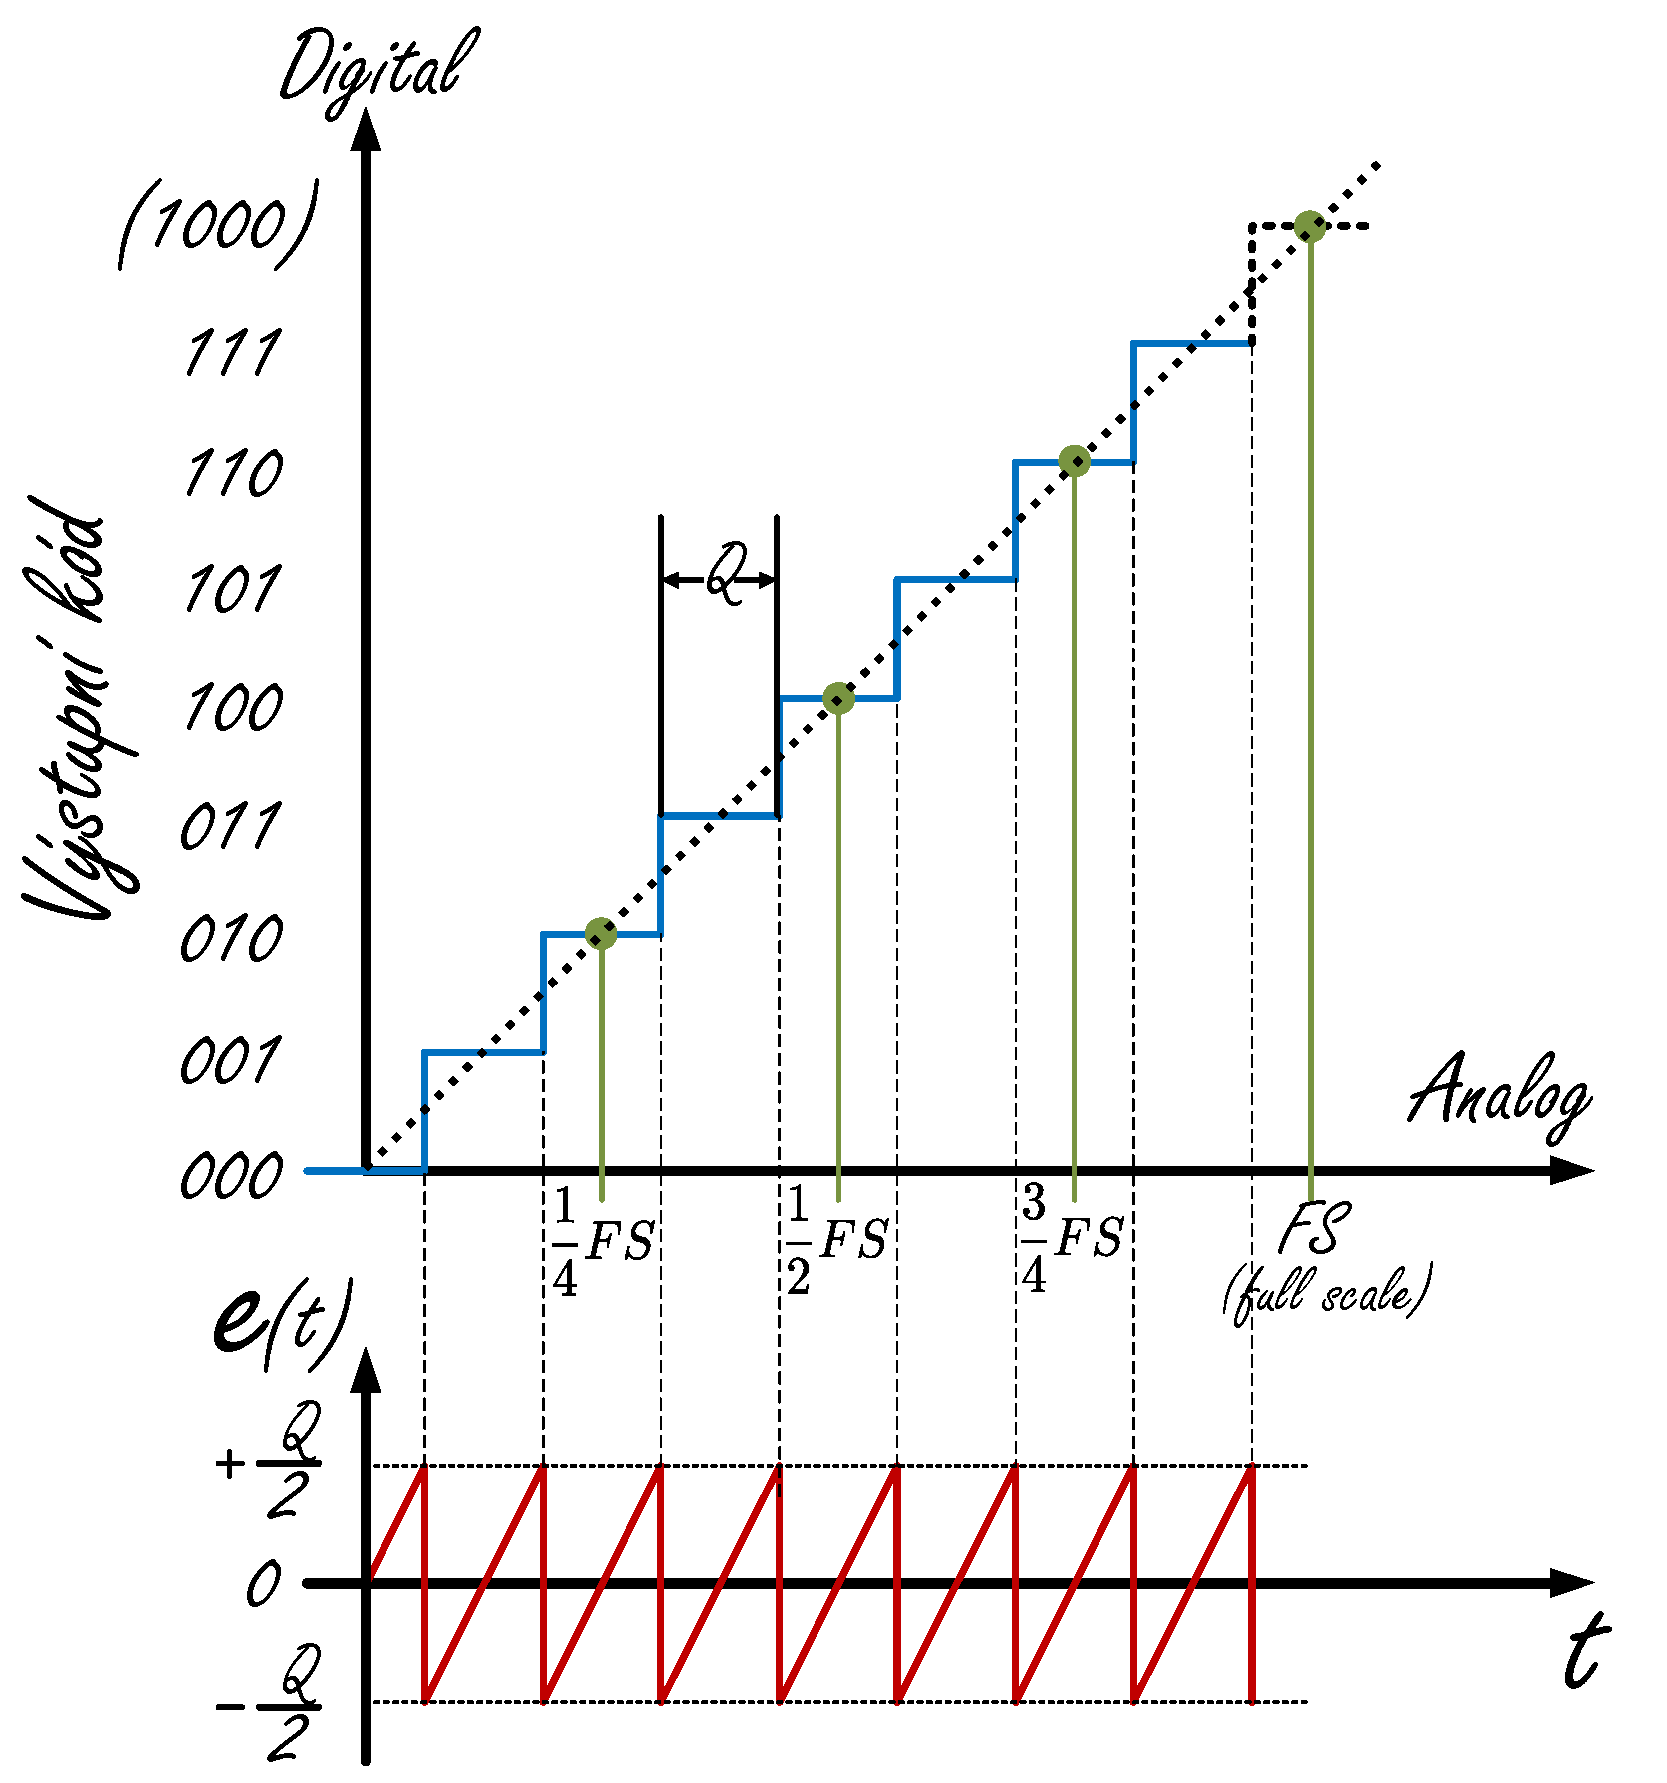
\includegraphics[width=0.8\linewidth]{AD_kvantizacni_chyba.pdf}
        \caption[Převodní charakteristika ideálních převodníků]{Převodní charakteristika 
                 ideálních převodníků a závislost chyby kvantizace na vstupní analogové hodnotě}
        \label{AES:fig_AD_kvantizacni_chyba}
      \end{figure}

      Z výše uvedeného plyne, že okamžitá hodnota kvantizační chyby $\varepsilon_q(t) = y(t) - x(t)$ může dosáhnout rozkmitu maximálně $\pm \frac{Q}{2}$ a jelikož předpokládáme rovnoměrné rozložení hodnot, je hustota pravděpodobnosti amplitud rovna $\frac{1}{Q}$.

      \emph{Kvantizační šum $\sigma^2$ je definován jako výkon (rozptyl) střídavé složky kvantizační chyby $\varepsilon_q$ a jeho efektivní hodnotu $\sigma$ můžeme odvodit pomocí věty o druhém centrálním momentu nebo výpočtem efektivní hodnoty v časové oblasti.}

        \begin{figure}[ht!]
          \centering
          \subfloat[Hustota pravděpodobnosti kvantizačního šumu]{\label{AES:fig_kvant_sum1}
            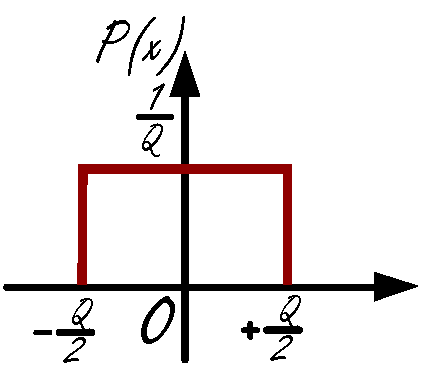
\includegraphics[width=0.4\linewidth]{AD_kvantizacni_sum1.pdf}}
          \subfloat[Kvantizační šum jako funkce času]{\label{AES:fig_kvant_sum2}
            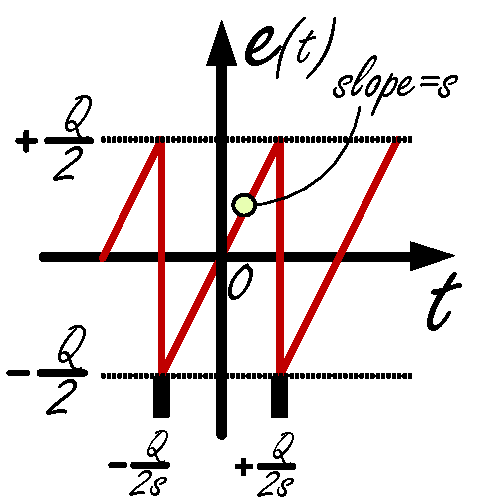
\includegraphics[width=0.4\linewidth]{AD_kvantizacni_sum2.pdf}}
          \caption{K odvození efektivní hodnoty kvantizačního šumu}
          \label{AES:fig_kvant_sum}
        \end{figure}

        \begin{enumerate}
          \item V pravděpodobnostním počtu je K-tý moment definován jako: 
                \begin{align*}
                  M_k  &= \int_{-\infty}^{\infty} x^k p(x)dx  \\
                  \shortintertext{tedy}                       \\
                  e(t) &= \int_{-\frac{Q}{2}}^{+\frac{Q}{2}}(x - x_0)^2p(x)dx = 
                                 \frac{1}{Q}\int_{-\frac{Q}{2}}^{+\frac{Q}{2}}x^2dx = \frac{Q^2}{12}
                \end{align*}
          \item V časové oblasti má kvantizační šum pilový průběh viz obr.    
                \ref{AES:fig_kvant_sum2}. Z  definičního integrálu efektivní hodnoty dostaneme $$ 
                \overline{e^2(t)} =               
                \frac{s}{Q}\int_{-\frac{Q}{2}}^{+\frac{Q}{2}}(st)^2dt = \frac{Q^2}{12}.$$ Též 
                můžeme využít znalosti efektivní hodnoty pro průběh tohoto typu: 
                $\frac{U_m}{\sqrt{3}}$ a dosazením za $U_m =\frac{Q}{2}$ získáme opět stejný 
                výsledek jako při výpočtu integrálu
        \end{enumerate}

        Tedy efektivní hodnota kvantizačního šumu ideálního N-bitového převodníku je:
        \begin{equation}\label{AES:eq_ef_kv_sumu}
            e(t) = \frac{Q}{\sqrt{12}}
        \end{equation}
        Předpokládejme na vstupu převodníku ustálený harmonický signál o amplitudě $X$. Dále 
        předpokládejme, že signál s amplitudou $X_m$ by pokryl celý rozsah převodníku $FS$. Pak se 
        dá ze vztahu \ref{AES:eq_SNR} vyjádřit odstup signálu od šumu \texttt{SNR} ideálního 
        \emph{N-bitového} převodníku jako podíl jejich výkonů resp. kvadrátu efektivních hodnot 
        signálu a šumu v decibelech vztahem
        \begin{align*}
          SNR      &= \frac{P_{signal}}{P_{noise}} =     
                      \left(\frac{A_{signal}}{A_{noise}}\right)^2         \\
          SNR_{dB} &= 10\log\frac{P_{signal}}{P_{noise}} =       
                      10\log\left(\frac{A_{signal}}{A_{noise}}\right)^2   \\
                   &= 20\log\frac{A_{signal}}{A_{noise}}                  
        \end{align*}
        \begin{equation}\label{AES:eq_SNR_N}
            SNR  = 1,76 + 6,02N + 20log\left(\frac{X}{X_m}\right)
        \end{equation}

        Lze tedy říci, že každý bit navíc v digitálním výstupu A/D převodníku přinese zlepšení 
        odstupu signálu od šumu o \texttt{6 dB}. Naproti tomu je třeba vědět, že uvedený výraz 
        počítá s harmonickým signálem různého rozkmitu. Při zmenšování amplitudy bude relativní 
        podíl šumu v signálu vyšší. Poměry se také mohou velmi změnit, když signál nebude mít 
        harmonický charakter.

      \subsubsection{Odstup signálu od šumu}\label{AES:cap_SNR}
        Z předchozí kapitoly víme, že SNR je definován jako poměr výkonu signálu k výkonu šumu ($v\acute{y}kon = ef. hodnota^2$). Pro samotný kvantizační šum platí:
        \begin{align}
          SNR_{dB} &= 10\log\left(\frac{\dfrac{2^N}{2\cdot\sqrt{2}}\cdot     
                                        Q}{\dfrac{Q}{\sqrt{12}}}\right)^2          \nonumber \\
                   &= N20\log2 + 20\log\frac{\sqrt{12}}{2\cdot\sqrt{12}}           \nonumber \\ 
          SNR_{dB} &= 6,02\cdot N + 1,76dB
        \end{align}

        \begin{figure}[ht!]
            \centering
            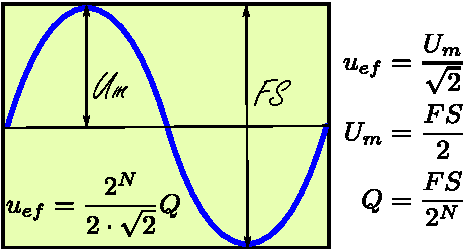
\includegraphics[width=0.6\linewidth]{AD_SNR.pdf}
            \caption{}
            \label{AES:fig_SNR}
        \end{figure}

        Tato hodnota platí pouze pro ideální převodník pouze s kvantizační chybou, a sinusový 
        signál s rozkmitem přes celý rozsah převodníku.  Skutečný převodník má ovšem vlivem dalších 
        chyb \texttt{SNR} menší než \texttt{SNR} určený pouze pro kvantizační šum. Tato hodnota se 
        nazývá \texttt{SINAD} nebo \texttt{SNDR} - \emph{Signal-to-Noise and Distortion ratio}.

        Známe-li \texttt{SNR} skutečného převodníku, můžeme určit počet efektivních bitu $N_{ef}$ 
        tzn. \emph{efektivní rozlišitelnost převodníku}. Ten je vždy menší než $N$.
        \begin{equation}\label{AES_eq_N_ef}
            N_ef = \frac{SNR - 1,76}{6,02}
        \end{equation}
        
  \section{Principy A/D převodníků}
      Převod analogového signálu na číslo lze uskutečnit několika různými postupy:\cite{Neumann}
      \begin{enumerate}
        \item Vstupní signál se porovnává s kvantovanou referenční veličinou a komparátory okamžitě 
              vyhodnotí, který z nich je větší. Přímým výstupním údajem je binární číslicové slovo.
        \item Vstupní signál i referenční veličina se v určité časové sekvenci zavádějí do   
              integrátoru a komparátor na jeho výstupu určuje sekvenci impulsů, vypovídající o 
              hodnotě vstupní analogové veličiny. Informací o vstupní veličině dále přenáší počet 
              impulsu, jejich kmitočet nebo kódovaná sekvence impulsů. Tato informace může být 
              převedena číslicovým blokem (obvykle blokem DSP) na binární číslicové slovo.
      \end{enumerate}

      Bývá také používáno třídění na \emph{převodníky s přímým a nepřímým vyhodnocení analogové 
      veličiny}.
      \begin{itemize}
        \item \texttt{Převodníky s přímým vyhodnocením} porovnávají hodnoty analogové veličiny s  
              vybranými kvantizačními úrovněmi současně nebo postupně, a to tak, že každá úroveň má 
              vlastní komparátor. K těmto převodníkům patří \emph{převodníky paralelní a kaskádní}.
        \item \texttt{K nepřímému převodu} můžeme využít postupného provoláváním vstupní  
              ve\-li\-či\-ny s vhodnými vzorky referenčního napětí, dodávanými na vstup jediného 
              komparátoru v pořadí a velikosti řízené logickými obvody. U těchto převodníků je 
              vstupní analogová veličina porovnávaná s výstupní veličinou převodníku \texttt{D/A}, 
              přičemž je číslicový vstup tohoto převodníku měněn tak, aby se obě veličiny k sobě 
              přibližovaly. Pokud se k sobě dostatečně přiblíží, je převod ukončen. I zde jsou v 
              podstatě jen dvě jednoduché možnosti přibližování výstup převodníku \texttt{D/A} k 
              určité úrovni vstupní veličiny: buď se přibližování děje se stálým krokem, kdy jde o 
              krokování po jednotlivých kvantovacích úrovních (\emph{převodníky sledovací}), nebo 
              postupnou aproximací (\emph{převodníky aproximační}), kdy první krok rozhoduje o 
              hodnotě \texttt{MSB}, další kroky porovnávají binárně zmenšované hodnoty 
              odpovídající jednotlivým binárním řádům s tím, že poslední krok určí hodnotu \texttt{LSB}.
        \item Jinou možností nepřímého převodu A/D je převést hodnotu vstupní veličiny na takový  
              parametr pomocného signálu, který se pak dá snadno převést na číslicový údaj. Tímto 
              parametrem je nejčastěji kmitočet, jindy to může být i počet impulzů v určitém 
              časovém intervalu nebo kódovaná sekvence impulzů. U těchto převodníků j kromě 
              komparátoru typickým funkčním blokem integrátor.
      \end{itemize}

  \section{Převod číslicového signálu na analogový}
    Číslicově-analogové převodníky převádějí číslicový signál zpravidla ve formě binárně kódovaného čísla na proud nebo napětí.
    \begin{equation}\label{AES_eq_DA}
        U_A = D \cdot U_{REF} \quad  I_A = D \cdot I_{REF}
    \end{equation}
    kde $U_{REF}, I_{REF}$ jsou referenční napětí a proud určující rozsah výstupní veličiny. Je-li 
    referenční napětí konstantní jedná se o klasické převodníky \texttt{DAC}. Při proměnném 
    referenčním napětí se jedná o násobící převodníky \texttt{MDAC}, které realizují násobení 
    časově proměnného referenčního spojitého a vstupního číslicového signálu.  Hodnota číslicového 
    signálu $D$ se vyjadřuje ve dvojkovém nebo dvojkově desítkovém (\texttt{BCD}) kódu.
    Ve dvojkovém kódu:
    \begin{equation}\label{AES:eq_DA_Dbin}
        D_B =\sum_{i=1}^n a_i\cdot2^{-i}
    \end{equation}
    $n$ je počet bitů dvojkového čísla. Bit $a_1$ s nejvyšší vahou $1/2$ se označuje \textbf{MSB}, 
    bit  $a_n$ s nejnižší vahou $2^{-n}$  se označuje \textbf{LSB}. \emph{Maximální hodnota 
    číslicového signálu $D_{MAX} = 1 - 2^{-n}$ a proto maximální hodnota výstupní veličiny je vždy 
    o 1 LSB menší, než je rozsah převodníku.} Veličina $2^{-n}\cdot U_{REF}$, resp. $2^{-n}\cdot 
    I_{REF}$ se nazývá \textbf{kvantum referenčního napětí nebo proudu} a určuje 
    \textbf{rozlišitelnost} převodníku. Převodní funkci D/A převodníku můžeme v případě 
    binárního kódu vyjádřit vztahem
    \begin{equation}\label{AES:eq_DA_bin}
        U_A = U_{REF}\cdot\left(a_{n}2^{-n} + a_{n-1}2^{-(n-1)} + \cdots + a_12^{-1}\right)
    \end{equation}
    Statické vlastnosti \texttt{D/A} převodníku jsou určeny převodní charakteristikou, která je 
    obvykle lineární (obr. \ref{AES:fig_DA_prevodni_charka}). Převodní charakteristika reálného DA 
    převodníku je zatížena chybou nuly, chybou zisku, integrální a diferenciální nelinearitou a 
    monotónností převodu.

    Z převodní charakteristiky lze tedy určit následující parametry převodníku:
    \begin{itemize}
      \item Chybu nuly (posunu) $\varepsilon_0$
           \begin{equation}\label{AES_eq_chyba_nuly}
             \varepsilon_0 = \frac{\Delta U_0}{U_{REF}}
           \end{equation}
      \item Chybu měřítka (zesílení) $\varepsilon_m$
           \begin{equation}\label{AES_eq_chyba_zesileni}
             \varepsilon_m = \frac{\Delta U_m - \Delta U_0}{U_{REF}}
           \end{equation}
      \item Integrální nelinearitu $I_{NL}$ jako maximální odchylku výstupního napětí sku\-teč\-né\-ho 
      převodníku od ideální hodnoty v celém rozsahu převodníku
           \begin{equation}\label{AES_eq_chyba_integralni}
             I_{NL} = \frac{\max\Delta U_n}{U_{REF}}
           \end{equation}
    \end{itemize}

    \begin{figure}[ht!]
       \centering
       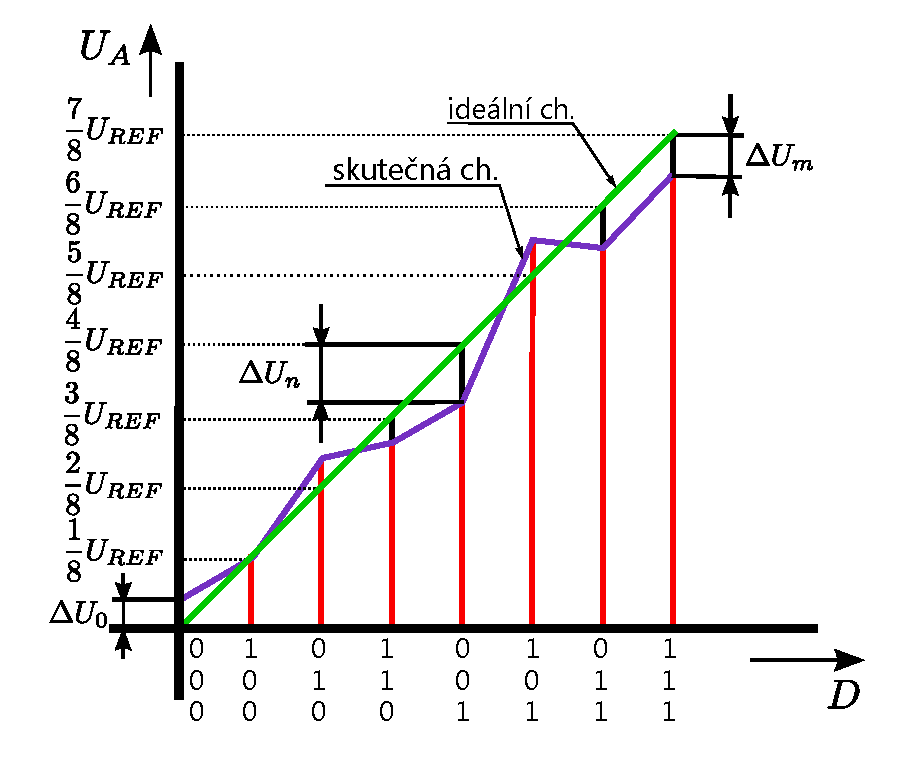
\includegraphics[width=0.8\linewidth]{DA_prevodni_charka.pdf}
       \caption[Převodní charakteristika DA převodníku]{Statická převodní charakteristika 3 bitového DA převodníku}
       \label{AES:fig_DA_prevodni_charka}
    \end{figure}

    Všechny tyto chyby se vyjadřují buď v procentech jmenovitého rozsahu $U_{REF}$ 
    pře\-vod\-ní\-ku, nebo v jednotkách ideální kvantizační úrovně (kvanta) $q = 2^{-n}\cdot 
    U_{REF}$.

    Dynamické vlastnosti D/A převodníku jsou charakterizovány \textbf{dobou ustálení} $T_u$ (obr. 
    \ref{AES:fig_DA_Tu}), potřebnou k ustálení výstupního signálu na jmenovitou hodnotu se zadanou 
    chybou $\Delta U$ obvykle $\pm0.5 LSB$.

    U násobících D/A převodníků se navíc určuje kmitočtový rozsah referenčního napětí kmitočtem 
    $f_m$, při kterém poklesne výstupní napětí převodníku o $3 dB$ oproti stejnosměrnému napětí při 
    maximální hodnotě číslicového signálu.

    \begin{figure}[ht!]
       \centering
       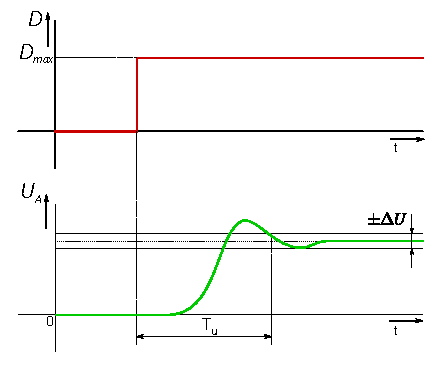
\includegraphics[width=0.4\textwidth]{DA_doba_Tu.pdf}
       \caption[Doba ustálení DA převodníku]{Doba ustálení $T_a$ DA převodníku. Je to celková   
                doba od změny vstupního kódu do ustálení analogového výstupu s přesností 
       $\pm\frac{1}{2}LSB$}
       \label{AES:fig_DA_Tu}
    \end{figure}

    \subsection{DA převodník DAC0800}
      D/A převodník DAC0800 je velmi rychlý násobící D/A převodník s rozlišením 8 bitů, pracující 
      na principu spínaných proudových zdrojů (viz obr. \ref{AES:fig_DAC0800_blok_sch}).
      \begin{figure}[ht!]
        \centering
        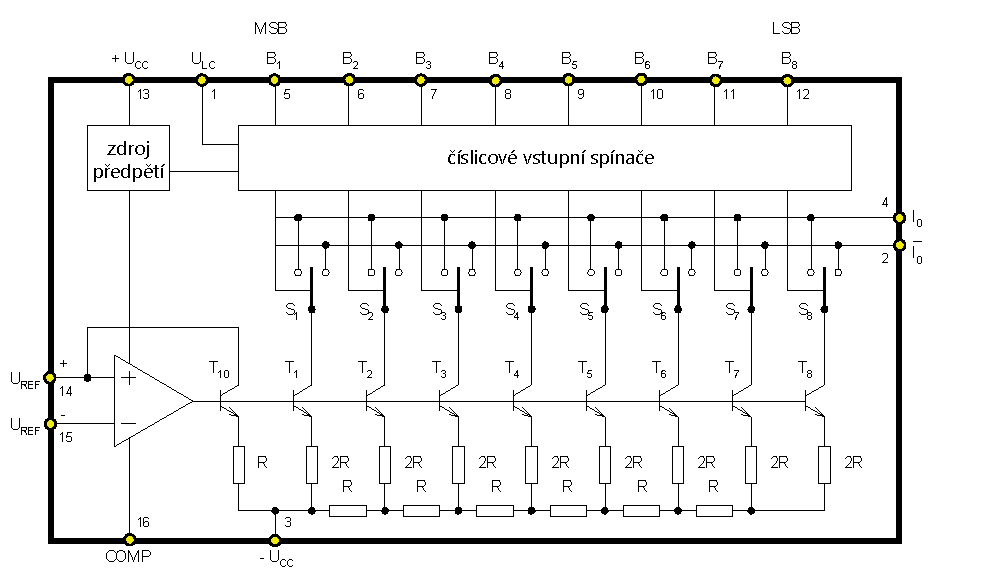
\includegraphics[width=1\linewidth]{DAC0800_block_diagram.pdf}
        \caption[Blokové schéma DAC0800]{Blokové schéma DA převodníku DAC0800}
        \label{AES:fig_DAC0800_blok_sch}
      \end{figure}

      Vstup převodníku je proudový, proudový výstup je řešen jako komplementární. IO v sobě slučuje 
      proudové spínače, váhové odpory a řídící zesilovač. Analogová reference, přesné vnější 
      odpory, korekční kondenzátor a výstupní zesilovač se připojují vně převodníku. Převodník 
      \texttt{DAC0800} generuje váhové proudy do komplementárních proudových sběrnic $I_0$ a 
      $\overline{I}_0$ prostřednictvím spínaných proudových zdrojů s tranzistory $T_1$ až $T_8$ a 
      odporovou sítí $R-2R$ viz obr. \ref{AES:fig_DAC0800_blok_sch}. Při úrovni \texttt{H} na 
      číslicových vstupech $B_1$ až $B_8$ připojí spínače $S_1$ až $S_8$ příslušné váhové proudy na 
      výstup $I_0$ a při úrovni \texttt{L} na výstup $\overline{I}_0$.

      Nezávislost váhových proudů na teplotních změnách zajišťuje referenční zdroj prou\-du s 
      tranzistorem $T_{10}$ a zesilovačem \texttt{Z}, ke kterému se připojuje referenční proud o 
      jmenovité hodnotě $2 mA$. Kondenzátor s kapacitou $10 nF$ připojený mezi vývody \texttt{3} a 
      \texttt{16} slouží ke kmitočtové kompenzaci zesilovače \texttt{Z}. Číslicové vstupy $S_1$ až 
      $B_8$ řídí spínače $S_1$ až $S_8$ prostřednictvím převodníku úrovní, přičemž svorkou $V_{LC}$ 
      (pin 1) lze volit slučitelnost převodníku s obvody TTL, DTL, CMOS atd.

      Vstupní referenční proud $I_{REF}$ je odvozen pomocí vnějšího přesného odporu $R_{REF}$ ze 
      zdroje referenčního napětí $U_{REF}$. Souběh referenčního proudu a plného výstupního proudu 
      $I_{FS}$ je zachován v rozpětí dvou dekád proměnné unipolární reference a umožňuje použít IO 
      též jako násobící převodník. Výstupní proudy $I_0$, $\overline{I}_0$ z vysokoimpedančních 
      výstupů se mohou využívat přímo nebo pomocí vnějších odporů, popřípadě pomocí \texttt{OZ}, se 
      mohou převést na napětí. Převodník pracuje se vstupním přímým binárním kódem při využití 
      přímého proudového výstupu $I_0$ nebo se vstupním komplementárním binárním kódem, využije-li 
      se doplňkový proudový výstup $\overline{I}_0$. Rozhodovací úroveň číslicových vstupů lze z 
      vnějšku nastavit na potřebnou hodnotu. Proto lze k řízení převodníku \texttt{DAC0800} použít 
      všechny běžně používané řady log. obvodů.

      \begin{figure}[ht!]
        \centering
        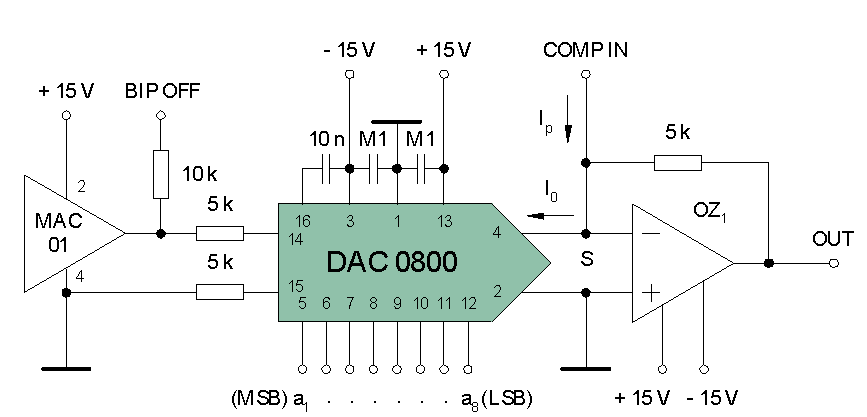
\includegraphics[width=1\linewidth]{DAC0800_sch1.pdf}
        \caption[Zapojení převodníku DAC0800]{Příklad zapojení převodníku DAC0800}
        \label{AES:fig_DAC0800_sch1}
      \end{figure}

      Příklad zapojení D/A převodníku je na obr. \ref{AES:fig_DAC0800_sch1}. Obsahuje kromě 
      vlastního D/A převodníku \texttt{DAC0800} zdroj referenčního napětí \texttt{MAC01} se 
      jmenovitým referenčním napětím +10 V a invertor se zesilovačem, pracujícím ve funkci 
      převodníku proudu na napětí pro realizaci napěťového výstupu převodníku. Funkce je 
      následující: Napětí $+10 V$ z \texttt{ MAC01} je pomocí odporu $5k\Omega$ převedeno na proud 
      $I_{REF} = 2 mA$, který je přiveden do kladného referenčního vstupu \texttt{DAC0800}, kde je 
      vynásoben nastavenou hodnotou číslicového signálu, zadanou pomocí osmi dvoupolohových 
      přepínačů. Poté se proud max $-2\cdot\left(1 - 2^{-8}\right) mA$ objeví na výstupu $I_0$ 
      a invertující zesilovač převede na odpovídající napětí. Zpětnovazební rezistor zesilovače 
      $5k\Omega$ určuje rozsah výstupního napětí 0 až 10 V (unipolární režim). Jsou-li svorky 
      \texttt{BIP OFF} a \texttt{COMP IN} propojeny, pak do sčítacího bodu \emph{S} je přiveden 
      proud $I_p = I_{REF}/2$ tj. 1 mA  ($I_p = 10 V/10 k\Omega$) opačného směru než $I_0$, který 
      způsobí trvalý posun výstupní napěťové úrovně převodníku o $-5 V$, takže rozsah převodníku 
      bude $\pm5 V$ (bipolární režim) a hodnota výstupního napětí je určena dvojkovým kódem s 
      posunutím (MSB určuje polaritu výstupního napětí).

} % tikzset
%---------------------------------------------------------------------------------------------------
\printbibliography[title={Seznam literatury}, heading=subbibliography]
\addcontentsline{toc}{section}{Seznam literatury} 
  % % !TeX spellcheck = cs_CZ
%---------------------------------------------------------------------------------------------------
% file opamp.tex
%---------------------------------------------------------------------------------------------------
%================================ Kapitola: Zesilovače==============================================
\setchaptertoc
\chapter{Operační zesilovače}\label{aesIchIII}

  \section{Základní pojmy}\label{aesIchIIIsecI}
    \subsection{Operační zesilovač}\label{aesIchIIIsecIssecI}
      \emph{Operační zesilovače} (\texttt{OZ}, aj: \texttt{opamp}) původně vznikly jako složité
      elektronické obvody pro náročné použití při zpracování analogových (spojitě se měnících)
      stejnosměrných a nízkofrekvenčních střídavých signálů v analogových počítačích, ve kterých
      realizovaly matematické operace. Aby se konstrukce analogových počítačů co nejvíce
      zjednodušila, bylo třeba unifikovat jejich jednotlivé části. Nejdůležitějším prvkem byl právě
      operační (dříve také nazývaný počítací) zesilovač. Protože měl vyhovět nejrůznějším
      požadavkům, bylo nutné, aby měl některé speciální vlastnosti \cite[s.~12]{Belza2004}. 

      \begin{figure}[ht!]  %\ref{aes:fig044}
        \centering
        \luafigure[0.4]{aes_fig044.jpg}
        \caption{První komerčně dostupný operační zesilovač \texttt{K2-W} z roku 1953
                \cite[s.~H.20]{Jung2005}}
        \label{aes:fig044}
      \end{figure} 

      Historie vývoje operačních zesilovačů je spjata s vývojem elektronek již od doby druhé světové
      války a je velice dobře popsána v příručce od \texttt{Analog Devices} \cite{Jung2005}. Vývoj
      je zde dokumentován také citací patentů. Tato éra vrcholí v roce 1953, kdy G. A. Philbrick
      uvedl na trh první komerčně dostupný operační zesilovač \texttt{K2-W} (obr. \ref{aes:fig044}).
      Elektronky byly později nahrazeny tranzistory a polovodičovými diodami. 
      
      Moderní polovodičová technologie umožnila vznik \texttt{OZ} v podobě levného integrovaného
      obvodu s malým počtem vývodů, který má nepatrnou spotřebu, je odolný proti přetížení a
      umožňuje jednoduše realizovat nejrůznější elektronická zařízení.
    
      V dnešním pojetí je možné vymezit operační zesilovač jako stejnosměrný zesilovač s velkým
      zesílením a malým vlastním rušením, schopný stabilní činnosti v uzavřené zpětnovazební smyčce.
      Přesným význam bude vyložen v následujících kapitolách. Zde jen poznamenejme, že přívlastkem
      \emph{stejnosměrný} není myšleno horní omezení dynamických vlastností operačního zeslovače,
      nybrž naopak rozšíření spektra zpracovávaných signálů k nulové frekvenci, k nekonečně dlouhým
      periodám.\cite[s.~5]{Dostal}.

      \begin{figure}[ht!]  %\ref{aes:fig041}
        \centering
          \subcaptionbox{\label{aes:fig041a}}{\luafigure[0.33]{aes_fig041a.pdf}}                                                  
          \subcaptionbox{\label{aes:fig041b}}{\luafigure[0.33]{aes_fig041b.pdf}}                    
          \subcaptionbox{\label{aes:fig041c}}{\luafigure[0.33]{aes_fig041c.pdf}}
        \caption{Symbolická značka OZ s vyznačenými signálovými svorkami (a) 
                a skutečná realizace zemní svorky (b, c) (\cite[s.~5]{Dostal})}
        \label{aes:fig041}
      \end{figure}

      Směr signálového toku operačním zesilovačem (dále jen OZ) od vstupu k výstupu je vyznačen
      trojúhelníkovým tvarem jeho symbolické značky na obr. \ref{aes:fig041a}. Tři ze čtyř
      znázorněných svorek představují tři signálové vývody skutečného operačního zesilovače a
      nazývají se \emph{invertující vstup, neinvertující vstup} a \emph{výstup}. Čtvrtá signálová
      svorka - zem - může být skutečná (obr. \ref{aes:fig041b}) nebo jen pomyslná (společná zem
      napájecích zdrojů na obr. \ref{aes:fig041c}), avšak v každém případě představuje symbolicky
      skupinu alespoň dvou napájecích vývodů určených pro přívod energie.  

      \begin{figure}[ht!]  %\ref{aes:fig042}
        \centering
        \subcaptionbox{\label{aes:fig042a}}{\luafigure[0.45]{aes_fig042a.jpg}}                                                 
        \subcaptionbox{\label{aes:fig042b}}{\luafigure[0.45]{aes_fig042b.jpg}}                    
        \caption{Přiřazení a orientace vstupních a výstupních napětí a proudů (a). Ve zjednodušeném 
                způsobu kreslení se zemní svorka vynechává (b). (\cite[s.~6]{Dostal})}
        \label{aes:fig042}
      \end{figure}

      Vedle signálových a napájecích vývodů má operační zesilovač podle potřeby ještě další vývody,
      určené např. pro úpravu dynamických charakteristik, pro nulování ofsetu, pro nastavení
      klidového odběru apod.

      Zemní signálová svorka tvoří referenční bod pro zbývající tři signálové svorky. Přiřazení
      kladných smyslů vstupních napětí \(u^-\), \(u^+\), výstupního napětí \(u_o\), vstupních proudů
      \(i^-\), \(i^+\) a výstupního proudu \(i_0\), ukazuje obr. \ref{aes:fig042a}. Nehrozí-li
      nedorozumění, může se zem ze značky zesilovače vypustit. Svorková napětí, vztažená i nadále k
      zemi, se pak vyznačí jen připsáním symbolu (obr. \ref{aes:fig042b}).

      Absolutní velikosti signálových napětí \(u^-\), \(u^+\) a \(u_o\) jsou omezeny napětím
      napájecích zdrojů. U zesilovačů s dvojitým napájením se používají dvě zpravidla vzájemně
      opačná napájecí napětí \(U_s^+\) a \(U_s^-\) (obr. \ref{aes:fig041c}), rovná např.
      +\SI{+15}{\volt} a \SI{-15}{\volt}. Odpovídající rozkmit obou vstupních napětí a výstupního
      napětí je pak rovněž souměrný do obou polarit, např. v mezích \(\pm\)\SI{10}{\volt}. U
      zesilovačů s jednoduchým napájením se používá jedno napájecí napětí \(U_s\) (obr.
      \ref{aes:fig041b}), rovné např. \SI{5}{\volt}. Odpovídající rozkmit obou vstupních napětí a
      výstupního napětí je pak pouze do jedné polarity, např. v mezích \num{0}/+\SI{4}{\volt}.

      Výstupní proud \(i_0\), se přizpůsobuje zátěži. Ta může být pasivní i aktivní, s přípustnými
      pracovními body (\(u_o\), \(i_0\) ve všech čtyřech kvadrantech, v případě dvojitého napájení.

      Charakteristickou přenosovou vlastností operačního zesilovače je jeho velká citlivost k
      rozdílu obou vstupních napětí a necitlivost k jejich absolutní velikosti. Tato vlastnost
      přivádí k pojmům \textbf{souhlasného vstupního napětí} \(u_{cm}\) jako superponované společné
      složky obou vstupních napětí, kterou zesilovač potlačuje, a \textbf{diferenčního vstupního
      napětí} \(u_D\), na které zesilovač reaguje. Zatímco přiřazení diferenčního vstupního napětí
      je nasnadě (obr. \ref{aes:fig042a}),
      \begin{equation}\label{aes:eq026}
        u_D = u^- - u^+,
      \end{equation}
      jsou možnosti definice souhlasného vstupního  napětí neomezené, 
      \begin{equation}\label{aes:eq027}
        u_{CM} = u^+ + Ku_D,
      \end{equation}
      dané volitelností konstanty \(K\). Dvě prakticky používané volby jsou \(K=\frac{1}{2}\) a
      \(K=0\). První volba zachovává symetrii, 
      \begin{equation*}
        u_{CM} = \dfrac{u^- + u^+}{2},
      \end{equation*}
      ale vede k formálním obtížím při definici parametrů operačního zesilovače. Proto se dává
      přednost druhé volbě, při které je souhlasné vstupní napětí ztotožněno s napětím
      neinvertujícího vstupu: 
      \begin{equation*}
        u_{CM} = u^+,
      \end{equation*}
      Tato druhá volba je opodstatněná také funkcí uzavřené zpětnovazební smyčky v nejčastějších
      případech, ve kterých zastává neinvertující vstup úlohu vnucené reference, s níž se
      invertující vstup samočinně srovnává. Rozdíl mezi oběma definicemi je nadto prakticky
      nepodstatný vzhledem k nepatrné velikosti diferenčního vstupního napětí ve srovnání s rozsahem
      souhlasného vstupního napětí. 

      %--Zesílení Ideálního Operačního Zesiovače----------------------
      % !TeX spellcheck = cs_CZ
\begin{mdframed}[style=mdexam]
  \begin{example}\label{aes:exam004}
    Běžné OZ mají zesílení \(A = \numrange{20000}{2000000}\). Znamená to, že pro výstupní napětí
    \SI{10}{\V} je mezi kladným a záporným vstupem napětí \(u_D
    =\frac{\SI{10}{\V}}{\numrange{2000000}{20000}}\) = \SIrange{5}{500}{\uV}. V praxi to většinou
    znamená, že rozdílové napětí \(u_D\) považujeme za nulové pro jakékoliv výstupní napětí \(u_0\).
    Jak se později ukáže, tato úvaha je velmi důležitá. Podmínku \(u_D = 0\) se snažíme zajistit za
    všech okolností. Vede to k požadavku, aby zesílení ideálního OZ bylo nekonečně velké (u reálného
    co největší) (\cite[s.~14]{Puncochar1996}).    
  \end{example}
\end{mdframed}
      %---------------------------------------------------------------
    
    \subsection{Operační obvod}\label{aesIchIIIsecIssecII} 
      Samotný operační zesilovač je jen částí výsledného zařízení, i když zpravidla částí
      nejdůležitější. Nedílnou druhou, funkčně určující část tvoří vnější zpětnovazební síť. Obecné
      uspořádání s jedním operačním zesilovačem, signálovým zdrojem a zátěži ukazuje obr.
      \ref{aes:fig045}. Zpětnovazební síť, znázorněná vyšrafovaným obrazcem a sestavená z pasivních
      i aktivních elektronických a elektromechanických součástek, je ukončena vytknutými styčnými
      uzly, jejichž prostřednictvím je spojena se signálovými svorkami operačního zesilovače,
      signálového zdroje a zátěže. Celek operačního zesilovače, zpětnovazební sítě, signálového
      zdroje a zátěže tvoří operační obvod. Jeho vstupní veličinou je vstupní napětí \(u_s\) nebo
      vstupní proud \(i_s\) na svorkách signálového zdroje, jeho výstupní veličinou je výstupní
      napětí \(u_o\) nebo výstupní proud \(i_0\) na svorkách zátěže. Za povšimnutí stojí, že výstup
      operačního obvodu nemusí být obecně totožný s výstupem operačního zesilovače a zem zesilovače
      (zem napájecích zdrojů podle obr. \ref{aes:fig041b}, \ref{aes:fig041c} nemusí být přímo
      spojena s jednou svorkou signálového zdroje nebo zátěže, i když tomu tak zpravidla je.
      \begin{figure}[ht!] % \ref{aes:fig045}
        \centering
        \luafigure[1]{aes_fig045.png}
        \caption{Operační obvod s jedním operačním zesilovačem, jedním signálovým zdrojem a jednou 
                 zátěži. (\cite[s.~8]{Dostal})}
        \label{aes:fig045}
      \end{figure}

      S výjimkou operačních obvodů, které fungují jako referenční zdroj, oscilátor nebo
      multivibrátor, je výstupní veličina (\(u_0\), \(i_0\)) v jistém vztahu k vstupní veličině
      (\(u_s\), \(i_s\)). Tento vztah vyjádřený matematicky se nazývá operační rovnice obvodu.

      Nejcennější vlastností obvodů s operačními zesilovači je značná necitlivost operační rovnice
      jak k rozptylu parametrů samotného operačního zesilovače, tak ke změnám zátěže a často i
      signálového zdroje (ke změnám jejich zatěžovacího nebo vnitřního odporu). První skutečnost
      vede k definici ideálního operačního zesilovače (odst. \ref{aesIchIIIsecIssecIII}), druhá
      skutečnost vede ke zúženému chápání operačního obvodu jako pouhého spojení operačního
      zesilovače a zpětnovazební sítě. Necitlivost operační rovnice k vlastnostem přirozeně
      nestálého aktivního prvku - zesilovače - vtiskuje návrhu operačních obvodů rys matematické
      předvídatelnosti chování. Operační rovnice se tak stává spíše charakteristikou samotné
      zpětnovazební sítě.

      Operační obvod podle obr. \ref{aes:fig045} může být rozšířen připojením dalších signálových
      zdrojů, operačních zesilovačů a zátěží. Realizace zpětnovazební sítě nemusí být omezena jen na
      elektrické prostředky. Signálová smyčka se může uzavírat i přes jiné druhy signálu než
      elektrické napětí nebo elektrický proud: Přes magnetickou indukci, Lorentzovu sílu, mechanické
      napětí, deformaci a piezoelektrický náboj, přes teplo, teplotu a termoelektrické napětí, přes
      světlo a fotoemisní proud, přes polohu servomotoru a napětí polohového potenciometru apod.
      Jedinou, avšak zásadní svazující podmínkou je \emph{zachování} zpětnovazební stability
      výsledné uzavřené smyčky.


    \subsection{Ideální OZ a operační obvod}\label{aesIchIIIsecIssecIII}
      Paradoxním cílem, ke kterému směřuje snažení každého konstruktéra operačních zesilovačů, je
      vytvoření zesilovače v aplikaci neviditelného v tom smyslu, že neovlivňuje znění příslušné
      operační rovnice. Jeho abstrakcí je ideální operační zesilovač, užitečná představa, která
      umožňuje rychlou analýzu jmenovitého (zamýšleného) chování operačního obvodu nebo umožňuje
      syntézu operačního obvodu podle zadaného matematického nebo jen funkčního popisu, s výsledky
      použitelnými bezprostředně a přesně ve skutečné aplikaci. Skutečné operační zesilovače se
      svému ideálu v různé míře přibližují, přičemž těsnější přiblížení je při daném stavu
      technologie zpravidla zaplaceno větší obvodovou složitosti a vyšší cenou.
      \begin{itemize}[noitemsep]
        \item Ideální operační zesilovač je operační zesilovač s nulovým diferenčním vstupním
              napětím a s nulovými vstupními proudy pro jakékoliv výstupní vybuzení a jakékoliv
              souhlasné vstupní vybuzení: 
              \begin{equation}\label{aes:eq029}
                u_D, i^-, i^+ = 0 \quad\text{pro libovolné}\quad u_0, i_0, u_{CM}.
              \end{equation}
        \item ideální operační obvod je operační obvod vzniklý myšlenou náhradou skutečného
              operačního zesilovače ideálním operačním zesilovačem.     
        \item ideální operační rovnice je operační rovnice ideálního operačního obvodu.
      \end{itemize}

      Význam těchto abstrakcí oceníme v kapitole \ref{aesIchIVsecI}. Jak je vidět z rov.
      (\ref{aes:eq029}), je dokonalost operačního zesilovače určena dokonalosti jeho vstupní strany
      (odchylkou jeho diferenčního vstupního napětí a vstupních proudů od nuly).

      Řečeno jazykem kapitoly \ref{aesIchIIIsecII} má ideální operační zesilovač na všech
      frekvencích nekonečné zesilení, nekonečné potlačení souhlasného vstupního napětí, nekonečné
      souhlasné vstupní impedance a nulové vstupní rušivé zdroje, jak je rovněž možné vysledovat z
      rov. (\ref{aes:eq029}). Velikost diferenční vstupní impedance a výstupní impedance je vzhledem
      k nekonečnému zesílení nepodstatná. Protože však skutečné hodnoty těchto impedanci u
      skutečného zesilovače (s konečným zesílením) zhoršují dynamické chyby operačního obvodu,
      spojuje se s představou ideálního operačního zesilovače také nekonečná diferenční vstupní
      impedance a nulová výstupní impedance. Katalogový list ideálního operačního zesilovače tedy
      obsahuje samé nuly a nekonečna.

      Početní analýza operačního obvodu v určitém směru (např. výpočet šumu, zesílení) se velmi
      zjednoduší, jestliže se hned zpočátku zanedbají nepodstatné okolnosti, tj. jestliže se
      nepodstatné parametry operačního zesilovače idealizují. Idealizovaný operační zesilovač je
      operační zesilovač, jehož některé parametry mají ideální (nulovou nebo nekonečnou) velikost.

    \subsection{Shrnutí}\label{aesIchIIIsecIssecIV}
      \begin{enumerate}[noitemsep]
        \item Operační zesilovač má čtyři signálové svorky, i když se často kreslí jen tři - oba 
              vstupy a výstup. Čtvrtou signálovou svorkou je zem.
        \item Souhlasné napětí $u_{CM}$ je totožné s napětím jeho neinvertujícího vstupu $u^+$.
        \item Ideální operační zesilovač má za všech okolností nulové diferenční vstupní napětí a  
              nulové vstupní proudy.
      \end{enumerate}
    
  \section{Parametry OZ}\label{aesIchIIIsecII}
    Ideální operační zesilovač je nedosažitelná abstrakce. K posouzení kvality sku\-teč\-ného 
    operačního zesilovače slouží řada funkčních parametrů jako soubor dat, která lze zjistit 
    měřením na svorkách.
   
    Operační zesilovač, jako každý aktivní elektronický obvod, je obvod nelineární. Protože však
    prostředky analýzy nelineárních obvodů jsou omezené a pracné, je namístě otázka po přijatelné
    linearizaci. Její oprávněnost je podpořena tím, že parametry operačního zesilovače nevystupují v
    operační rovnici jako veličiny určující, nýbrž jako příčiny chyb, a že tedy jejich případná
    lineární aproximace zanáší jen nepřesnost druhého řádu, chybu v chybě.

    Odpověď na položenou otázku je příznivá. Všechny funkční charakteristiky operačního zesilovače
    připouštějí linearizaci bez přílišného odklonu od skutečnosti. Odpovídající kvazilineární
    parametry jsou podkladem lineárního modelu operačního zesilovače. Ostatní parametry jsou
    podstatné nelinearity, které tvoří meze jeho lineární oblasti.
    
    \subsection{Lineární model a parametry}\label{aesIchIIIsecIIssecI}
      Obr. \ref{aes:fig046} ukazuje úplný \emph{lineární model} operačního zesilovače. Se zřetelem k
      pozdější analýze chyb operačního obvodu je vhodné rozdělit znázorněné lineární parametry na
      \textbf{aditivní} a \textbf{multiplikativní}.
      \begin{itemize}[noitemsep]
        \item \textbf{Aditivní parametry} zahrnují náhradní rušivé zdroje náhodných fluktuací:
              \(E_R\), \(I_R^-\), \(I_R^+\), které způsobují aditivní chyby operačního obvodu
              nezávislé na jeho signálovém vybuzení.
        \item \textbf{Multiplikativní parametry} představované čtyřmi odpory \(R_D\), \(R^-_{CM}\),
              \(R^+_{CM}\), \(R_0\) a dvěma řídicími konstantami \(-A\), \(1/X\) závislých
              generátorů, vystihují pasivní a přenosové vlastnosti OZ a způsobují multiplikativní
              chyby operačních obvodu úměrné jeho signálovému vybuzení.
      \end{itemize}
      Vnitřní, na svorkách neměřitelný napěťový úbytek \(e_D\) na odporu \(R_D\) zastává v tomto
      modelu vazbu mezi vstupem a výstupem.
     
      Při práci s proměnnými signály v časové nebo ve frekvenční oblasti se význam použitých symbolů 
      vhodně rozšíří na impedance, operátorové přenosy apod.

      \begin{figure}[ht!] % \ref{aes:fig046}
        \centering
        \luafigure[1]{aes_fig046.pdf}
        \caption{Lineární model operačního zesilovače. (\cite[s.~14]{Dostal}}
        \label{aes:fig046}
      \end{figure}

      S obvodovým modelem na obr. \ref{aes:fig046} je rovnocenný \emph{matematický model},
      představovaný soustavou tří rovnic
      \begin{subequations}\label{aes:eq030}
        \begin{align}
          u_D &= E_R   + \dfrac{u_{CM}}{X} - \dfrac{u_0 + R_0i_0}{A},     \label{aes:eq030a}   \\
          i^- &= I_R^- + \dfrac{u_{CM}}{R_{CM}^-}
                       - \dfrac{u_0 + R_0i_0}{A(R_D\parallel R_{CM}^-)},  \label{aes:eq030b}   \\ 
          i^+ &= I_R^+ + \dfrac{u_{CM}}{R_{CM}^+}
                       + \dfrac{u_0 + R_0i_0}{AR_D}.                      \label{aes:eq030c}
        \end{align}
      \end{subequations}
      \(R_D\parallel R_{CM}^-\) značí paralelní kombinaci odporů \(R_D\) a \(R_{CM}^-\)
      
      Ekvivalence obou modelu je podložena Kirchhoffovými zákony psanými pro vstupní svorky
      operačního zesilovače při uvážení rovnosti \(e_D = -\frac{u_0 +R_0i_0}{A}\). Na vysvětlení to
      ukážeme pro vstupní proud \(i^-\). Proud tekoucí do invertujícího vstupu ma podle obr.
      \ref{aes:fig046} velikost
      \begin{equation*}
        i^- = I_R^- + \dfrac{u_{CM} + e_D}{R_{CM}^-} + \dfrac{e_D}{R_D} 
            = I_R^- + \dfrac{u_{CM}}{R_{CM}^-} + \dfrac{e_D}{(R_D\parallel R_{CM}^-)},
      \end{equation*}
      což souhlasí s rov. \ref{aes:eq030b}.

      Definice, které následují, předvádějí jednotlivé parametry lineárního modelu v termínech
      svorkových napětí a proudů a jejich změn. Každý parametr je znázorněn svým základním měřícím
      obvodem, který používá konceptu pomocného ideálního operačního zesilovače k imitování podmínek
      definice.

      Znění některých definici se poněkud liší od formulaci používaných výrobci operačních
      zesilovačů v katalogových listech. Katalogové údaje často představují spíše záruky řádného
      chování, které přísluší kombinovanému vlivu několika dílčích parametrů (např. zesílení při
      jmenovité zátěži), nebo vycházejí ze zavedených měřicích schémat, zatímco posláním této
      kapitoly je vytvoření jednodchého nástroje pro lineární a nelineární analýzu operačního obvodu
      v následující části \ref{aesIchIV}. Zmíněné odchylky jsou prakticky nepodstatné.
    
      \subsubsection{Vstupní rušivé zdroje}\label{aesIchIIIsecIIssecII}
        Reálné vlastnosti OZ se nejvíce projevují superponovanou výstupní chybovou složkou,
        způsobenou šumovými vlastnostmi součástek zesilovačef, jejich stárnutí a jejich citlivost na
        vnější vlivy. Největší podíl tohoto šumu v šírším smyslu slova přísluší vstupním obvodům.
        Pro kvantitativní posouzení je proto přirozená volba ekvivaletních vstupních rušivých
        zdrojů, virtuálně rovnocenných svým účinkém šumovému projevu skutečného OZ. Z praktických
        měřicích se ujala definice založená nikoliv na Ekvivalenci, nýbrž na kompenzaci skutečných a
        náhradních rušivých účinků.
        \begin{itemize}[noitemsep]
          \item \emph{Vstupní rušivé napětí} \(E_R\) je velikost diferenčního vstupního napětí při
                nulovém souhlasném vstupním napětí, která přísluší nulovému výstupnímu napětí
                naprázdno.
          \item \emph{Vstupní rušivý proud} \(I_R^-\), resp. \(I_R^+\) je velikost proudu
                invertujícího resp. neinvertujícího vstupu při nulovém souhlasném vstupním napětí,
                která přísluší nulovému výstupnímu napětí naprázdno.
        \end{itemize}

        Pro objasnění podmínek definice ukážeme, že takto definované vstupní rušivé zdroje jsou
        skutečně totožné s parametry \(E_R\), \(I_R^-\), \(I_R^+\) lineárního modelu na obr.
        \ref{aes:fig046}. 

        Ve stavu naprázdno je napěťový úbytek na odporu \(R_0\) nulový. Podmínka nulového výstupního
        napětí naprázdno (\(u_0=0\), \(i_0=0\), \(e_0=0\)) vede k nulovému vnitřnímu napětí \(e_D =
        - \frac{e_0}{A}\) a k nulovému vnitřnímu proudu \(\frac{e_D}{R_D}\) mezi oběma vstupy.
        Uzemněním neinvertujícího vstupu (\(u_{CM} = 0\)) se anuluje vnitřní závislé vstupní napětí
        \(e_{CM} = \frac{u_{CM}}{X}\) a anulují se také vnitřní proudy \(\frac{u_{CM}}{R_{CM}^+}\) a
        \(\frac{u_{CM} + e_D}{R_{CM}^-}\) tekoucí přes odpory \(R_{CM}^+\) a \(R_{CM}^-\).
        Odpovídající velikosti diferenčního vstupního napětí a vstupních proudů jsou tedy
        \begin{equation}\label{aes:eq031}
          u_D = E_R, \quad i^- = I_R^-, \quad i^+ = I_R^+,
        \end{equation}
        jak stanoví definice. Vztahy \ref{aes:eq031} plynou samozřejmě také z rov. \ref{aes:eq030}
        pro \(u_{CM}\), \(u_0\) a \(i_0 = 0\).

        \luagraphic[0.8]{aes_fig047.pdf}{Základní měřicí obvod pro měření vstupních rušivých zdrojů. 
        (\cite[s.~16]{Dostal})}{aes:fig047}

        Definice vstupních rušivých zdrojů korespondují se základním měřicím obvodem na obr.
        \ref{aes:fig047}. Výstup měřeného OZ s uzemněným neinvertujícím vstupem je snímám pomocným
        ideálním OZ, který zastává úlohu nezatěžujícího nulového indikátoru. Výstup tohoto pomocného
        zesilovače samočinně nastavuje invertující vstup měřeného OZ tak, že jeho výstupní napětí
        naprázdno je nulové. Podle definice je okamžitá velikost takto nastaveného vstupního napětí
        \(u_D\) rovna okamžité velikosti vstupního rušivého napětí \(E_R\) a okamžité velikosti
        vstupních proudů \(I_R^+\) a \(I_R^-\).

      \subsubsection{Vstupní ofset a drift}\label{aesIchIIIsecIIssecIII}
        Všimněme si blíže spektrálního složení vstupních rušivých zdrojů, obr. \ref{aes:fig048}. Pro
        přesnost aplikací jsou obvykle rozhodující stejnosměrné a velmi zvolna proměnné složky,
        souhrnně označované jako \textbf{vstupní ofset} operačního zesilovače. Pásmo frekvencí
        těchto kvazistejnosměrných složek se vymezuje rozsahem \num{0} až \SI{0.01}{\Hz}. Vstupní
        ofset zahrnuje vstupní zbytkové napětí \(E_{OS}\) (stejnosměrnou složku vstupního rušivého
        napětí \(E_R\) a vstupní klidové proudy \(I_B^+\), \(I_B^-\) (stejnosměrné složky vstupních
        rušivých proudů \(I_R^+\), \(I_R^-\)).
              
        Oba vstupní klidové proudy se obyčejně liší málo. K vyjádření jejich všeobecné shody se
        zavádějí odvozené pojmy, \textbf{(průměrný) vstupní klidový proud} \(I_B\) jako jejich
        průměr\footnote{Zaručený katalogový údaj vstupního klidového proudu \(I_B\) se vztahuje na
        každý proud \(I_B^-\) a \(I_B^+\) zvlášť, nikoliv na jejich průměr.} a \textbf{vstupní
        zbytkový proud} \(I_{OS}\) jako jejich rozdíl:
        \begin{equation}\label{aes:eq090}
          I_B = \dfrac{I_B^- + I_B^+}{2}, \quad I_{OS} = I_B^- - I_B^+.
        \end{equation}
        
        \begin{figure}[ht!] % \ref{aes:fig048}  aes_fig048.tex/jpg
          \centering
          \luafigure[1]{aes_fig048.pdf}
          \caption{Terminologie a symboly vstupních rušivých zdrojů. (\cite[s.~16]{Dostal})}
          \label{aes:fig048}
        \end{figure}

        Chybu způsobenou vstupním ofsetem operačního zesilovače je možné vynulovat vnějším zásahem
        do operačního zesilovače samotného nebo do zpětnovazební sítě. Pro přesnost aplikací je
        důležitější nestálost ofsetu, označovaná jako \textbf{vstupní drift}. Jak bude zřejmé z
        dalšího, rozumí se driftem nejčastěji poměr změny ofsetu ke změně příčinného vlivu. S
        výjimkou samovolných časových změn (stárnutí) jde o vratné změny ofsetu v závislosti na
        kolísání pracovního prostředí zesilovače - teploty okolí a napájecího napětí. Se zřetelem k
        této nestabilitě se označuje ofset příslušející \emph{standardním podmínkám} (teplota
        +\SI{25}{\degreeCelsius}, napájecí napětí např. +\SI{15}{\V}) jako počáteční ofset.
        
        \begin{figure}[ht!] % \ref{aes:fig049}
          \centering
          \luafigure[1]{aes_fig049.jpg}
          \caption{Teplotní závislost vstupního zbytkového napětí \(E_{OS}(T)\). Všechny tři
                  znázorněné průběhy přísluší vyhovujícím zesilovačům podle tříbodové definice
                  (2.4b), a přesto může diferenciální drift \(\der{E_{OS}}{T}\) překročit zaručenou
                  mez \(\pm(\Delta E_{OS}/\Delta T)_M\). (\cite[s.~17]{Dostal})}
          \label{aes:fig049}
        \end{figure}

        Typický průběh vstupního zbytkového napětí s teplotou ukazuje graf a na obr. 2.4. Pro
        jednoznačnost katalogových údajů a pro jednoduchost měření se k charakterizaci nelineární
        závislosti \(E_{OS}(T)\) zavádí \textbf{průměrný teplotní drift} vstupního zbytkového napětí
        \(\Delta E_{OS}/\Delta T\) v daném intervalu teplot \(\Delta T\) jako poměr změny vstupního
        zbytkového napětí mezi krajními teplotami tohoto intervalu k jeho délce.   
        
        V nejjednodušším případě se obě krajní teploty ztotožní s dolní a horní hranicí \(T_L\) a
        \(T_H\) rozsahu pracovních teplot a stanoví se průměrný drift

        \begin{subequations}\label{aes:eq039}
          \begin{align}
            \left.\frac{\Delta E_{OS}}{\Delta T}\right\rvert_{LH} &= 
                                    \dfrac{E_{OS_H} - E_{OS_L}}{T_H - T_L}, \label{aes:eq039a} \\
            \left.\frac{\Delta E_{OS}}{\Delta T}\right\rvert_{L0} &= 
                                    \dfrac{E_{OS_0} - E_{OS_L}}{T_0 - T_L}, \label{aes:eq039b} \\
            \left.\frac{\Delta E_{OS}}{\Delta T}\right\rvert_{0H} &= 
                                    \dfrac{E_{OS_H} - E_{OS_0}}{T_H - T_0}, \label{aes:eq039c}
          \end{align}
        \end{subequations}

        Důkladnější postup, který lépe postihuje nelinearity typu \(U\) (graf b na obr.
        \ref{aes:fig049}), spočívá v rozdělení pracovního rozsahu při standardní teplotě \(T_0\) na
        dva intervaly (\(T_L\), \(T_0\)) a (\(T_0\), \(T_H\)) a ve stanovení dvou dílčích průměrných
        driftů.

        V každém uvedeném způsobu se změřený a vypočtený teplotní drift podle rov.
        (\ref{aes:eq039a}) nebo (\ref{aes:eq039b}) resp. (\ref{aes:eq039c}) porovná s katalogovým
        údajem zaručeného driftu \((\Delta E_{OS}/\Delta T)_M\). Vyšrafovaný motýlek s hranicemi
        \((+\Delta E_{OS}/\Delta T)_M\) a \(-(\Delta E_{OS}/\Delta T)_M\) vymezuje pole, do kterého
        musí padnout koncové body teplotních průběhů \(E_{OS}(T)\) vyhovujících zesilovačů a ve
        kterém obvykle leží celý průběh \(E_{OS}(T)\).

        Průměrný drift je ukazatel dostatečně výstižný pouze u závislostí blízkých k závislosti
        lineární, protože si všímá jen koncových bodů a nepřihlíží k chování uvnitř intervalu: dva
        zesilovače s velmi odlišnými průběhy \(a\) a \(c\) na obr. \ref{aes:fig049} mají v intervalu
        (\(T_0\), \(T_H\)) tentýž průměrný drift. Průměrný drift může být ukazatel i hrubě
        zkreslující, jak ukazuje graf c na obr. \ref{aes:fig049}, který přísluší zesilovači s
        nulovým průměrným driftem v intervalu (\(T_L\), \(T_0\)), a přesto zesilovači značně
        teplotně citlivému.

        Obdobným způsobem se zavádí i průměrný teplotní drift vstupního klidového a vstupního
        zbytkového proudu \(\Delta I_B/\Delta T\) a \(\Delta I_{OS}/\Delta T\). Nelinearita
        závislosti \(I_B(T)\) a \(I_{OS}(T)\) je výraznější a pojem průměrného driftu je spornější.
        Často se proto udávají jen zaručené maximální hodnoty obou proudu \(I_B\) a \(I_{OS}\) při
        standardní teplotě a při mezních pracovních teplotách.

        Dosud probírané teplotní změny se týkaly operačního zesilovače jako celku. Mnohem
        nebezpečnější mohou být poměrně malé \emph{teplotní diference} mezi jeho kritickými částmi,
        způsobené cizími tepelnými zdroji nebo vlastním ohřevem (po zapnutí napájení, po změnách
        zátěže, po zahlcení vstupu) a projevující se porušením vnitřní teplotní kompenzace
        diferenčních zesilovacích stupňů nebo vznikem termoelektrických napětí. Zvlášť citlivé jsou
        levné typy operačních zesilovačů následkem nevyvážené tepelné zpětné vazby uvnitř
        polovodičového čipu.

        \emph{Kolísání napájení} je druhou podstatnou příčinou změny ofsetu. Citlivost na změnu
        napájecího napětí \(U_S\) se udává \emph{průměrným napájecím driftem} vstupního zbytkového
        napětí \(\Delta E_{OS}/\Delta U_S\), vstupního klidového proudu \(\Delta I_B/\Delta U_S\) a
        vstupního zbytkového proudu \(\Delta I_{OS}/\Delta U_S\). V případě zbytkového napětí je
        tento drift bezrozměrný (udávaný v \si{\micro\volt\per\volt}) a analogicky k potlačení
        souhlasného napětí, bývá někdy uváděn v převráceném poměru jako \emph{potlačení napájecího
        napětí} \(\Delta U_S/\Delta E_{OS}\) a udáván v decibelech.

        U zesilovačů s dvojitým napájením se změnou \(\Delta U_S\) obvykle rozumí změna jednoho z
        napájecích napětí \(U_S^+\) nebo \(U_S^-\). Je ovšem možné si představit i současnou a
        stejnou změnu obou napájecích napětí, a to ve stejném nebo v opačném smyslu, obecně však
        není možné předem odhadnout, která z těchto možností je nepříznivější. Souhrnně lze říci, že
        v porovnání s jinými elektronickými výrobky a při uvážení dosahované přesnosti je operační
        zesilovač ke svému napájení velmi tolerantní. Výsledná nestabilita napájecího napětí 1 \% až
        10 \% je vyhovující, pokud napájecí zdroj neslouží zároveň jako referenční zdroj operačního
        obvodu.

        Samovolná časová \emph{změna} ofsetu jako projev stárnutí je nevratná, a proto
        neopakovatelná. Z toho důvodu nemůže být ani rozumně zaručována, a bud" je udána typickou
        hodnotou sejmutou na ověřovacím souboru zesilovačů, nebo není uváděna vůbec. Analogicky k
        oběma předchozím driftům se používá poměrový údaj průměrného časového driftu vstupního
        zbytkového napětí \(\Delta E_{OS}/\Delta t\), vstupního klidového proudu \(\Delta I_B/\Delta
        t\) a vstupního zbytkového proudu \(\Delta I_{OS}/\Delta t\), vztažený na interval dne,
        měsíce nebo roku. Při interpretaci je však nutné pamatovat, že časový drift není
        kumulativní, a že tedy údaj příslušející jednomu intervalu není možné lineárně přenášet na
        interval kratší ani delší.

      \subsubsection{Vstupní šum}\label{aesIchIIIsecIIssecIV}
        \emph{Vlastní šum} OZ je udán \textbf{vstupním šumovým napětím} \(E_N\) (šumovou složkou
        vstupního rušivého napětí \(E_R\)) a \textbf{vstupními šumovými proudy} \(I_N^-\) a \(I_N^+\)
        (šumovými složkami vstupních rušivých proudů \(I_R^-\) a \(I_R^+\) ). Vzhledem ke statistické
        povaze šumu se obvykle uvádí pouze společný údaj \(I_N\) s významem \(I_N^-\) nebo \(I_N^+\).
        Šumové napětí a šumové proudy jsou zpravidla nezávislé, ale někdy mohou obsahovat korelované
        složky (např. šumové napěťové úbytky na ochranných sériových vstupních rezistorech, korelované
        s průtokem vstupních šumových proudů).
        
        Šumové Zdroje \(E_N\) a \(I_N\) se charakterizují integrálně nebo spektrální hustotou.
        Integrální údaj, který přísluší šumovým složkám z určitého frekvenčního pásma, představuje buď
        \emph{efektivní} (rms), nebo \emph{mezivrcholovou} (pp) hodnotu\footnote{Z anglického
        root-mean-square (rms) a peak-to-peak (pp)} šumového napětí \(E_N\) a šumového proudu \(I_N\)
        v dostatečném časovém intervalu. Definice efektivní hodnoty šumu vychází běžným způsobem z
        ekvivalence tepelných účinků, avšak mezivrcholová hodnota vyžaduje bližšího vysvětlení.

        \begin{figure}[ht!] % \ref{aes:fig050}
          \centering
          \luafigure[1]{aes_fig050.jpg}
          \caption{Vztah mezivrcholové a efektivní hodnoty šumového napětí \(E_N\) při Gaussově
                  rozdělení výchylek. Tabulka uvádí pravděpodobnost výskytu velkých výchylek, které
                  přesahují specifikovanou mezivrcholovou hodnotu, udanou jako nasobek efektivní
                  hodnoty (střední kvadratické výchylky) \(\sigma\). (\cite[s.~20]{Dostal})}
          \label{aes:fig050}
        \end{figure}

        Většina šumů sleduje Gaussovo (normální) rozdělení okamžitých výchylek, Znázorněné
        pravděpodobnostní rozdělovací křivkou na obr. \ref{aes:fig050}. Plocha pod rozdělovací křivkou
        mezi dvěma amplitudami \(u_N\) je rovna pravděpodobnosti výskytu okamžité velikosti šumu
        \(u_N(t)\) mezi těmito amplitudami. Přestože je pravděpodobnost výskytu velkých výchylek malá,
        jsou jakkoliv velké výchylky přece možné. Aby změřený údaj nezávisel na subjektu pozorovatele
        (na jeho trpělivosti, tj. na době pozorování nebo na délce záznamu), Zavádí se mezivrcholová
        hodnota šumového průběhu statisticky: Časová pravděpodobnost výskytu větších výchylek, které
        přesahují udanou mezivrcholovou hodnotu, je rovna dohodnutému procentu. Jinak řečeno,
        mezivrcholová hodnota udává šířku šumového pásu, ve kterém leží převažující část šumového
        průběhu, přičemž časová pravděpodobnost přesažení udaného šumového pásu (udané mezivrcholové
        hodnoty) je rovna dohodnutému procentu.

        Tabulka v obr. \ref{aes:fig050} přiřazuje několik údajů mezivrcholové hodnoty Gaussova šumu,
        vyjádřených v násobcích efektivní hodnoty (střední kvadratické výchylky) \(\sigma\). K rychlé
        orientaci pamatujeme, že mezivrcholová hodnota Gaussova šumu je asi \num{6}násobkem efektivní
        hodnoty, s pravděpodobností větších výchylek menší než 1 \%. Pro porovnání, mezivrcholová
        hodnota obdélníkového průběhu je \(2\times\sqrt{1} =2\)násobkem efektivní hodnoty,
        mezivrcholová hodnota sinusového průběhu je \(2\times\sqrt{2}\approx\num{2.8}\)násobkem
        efektivní hodnoty a mezivrcholová hodnota trojúhelníkového průběhu je
        \(2\times\sqrt{3}\approx\num{3.5}\)násobkem efektivní hodnoty, s pravděpodobností větších
        výchylek vesměs nulovou.
        
        \textbf{Spektrální hustoty} \(e_N\) a \(i_N\) šumového napětí \(E_N\) a šumového proudu
        \(I_N\) jsou diferenciálním vyjádřením závislosti efektivních hodnot \(E_N\) a \(I_N\) na
        oboru frekvence \(f\). Spektrální hustota šumového napětí \(e_N\) nebo šumového proudu \(i_N\)
        se definuje prostřednictvím spektrální hustoty \emph{šumového výkonu}, úměrného druhé mocnině
        efektivní hodnoty \(E_N\) nebo \(I_N\):
        \begin{equation}\label{aes:eq40}
          e_N^2 = \der{E_N^2}{f}, \quad\quad i_N^2 = \der{I_N^2}{f}.
        \end{equation}
        Rozměry spektrálních hustot \(e_N\) a \(i_N\) jsou \si[per-mode=symbol]
        {\V\per\sqrt{\Hz}} a \si[per-mode=symbol]{\A\per\sqrt{\Hz}}.

        Znalost frekvenčního průběhu spektrálních hustot \(e_N\) a \(i_N\) ve tvaru analytického
        výrazu, grafu nebo alespoň několika diskrétních hodnot umožňuje stanovení integrálního
        efektivního šumu ve sledovaném frekvenčním pásmu \(f_1\) až \(f_2\) analytickou nebo
        numerickou integrací výrazů
        \begin{equation}\label{aes:eq41}
          E_N^2 = \int_{f_1}^{f_2}{e_N^2}\dd{f}, \quad\quad I_N^2 = \int_{f_1}^{f_2}{i_N^2}\dd{f}.
        \end{equation}

        Od vlastního šumu operačního zesilovače, který jsme měli dosud na mysli, se odlišuje
        interferenční šum, vyvolaný vnějšími příčinami: šumem a zvlněním napájecích napětí, kapacitní
        a induktivní vazbou ze síťového rozvodu, z přesyceného transformátoru, z rozhlasových
        vysílačů, z mobilních telefonů, z vysokofrekvenčních indukčních pecí a z jiskřících kontaktů,
        mikrofoničností konstrukce a pohybem kabelů, cirkulujícím vzduchem a termoelektrickými
        napětími, povrchovými svody desek s plošnými spoji, kosmickými částicemi a zemními úbytky,
        atd.. Nejde o charakteristiku operačního zesilovače, ale spíše celého operačního obvodu v
        daném rušivém prostředí.

      \subsubsection{Zesílení. Diferenční vstupní odpor a výstupní odpor}\label{aesIchIIIsecIIssecV}
        Tři multiplikativní parametry \(A\), \(R_D\), \(R_0\) jsou sdruženy jednou zvláštností:
        Jejich přítomnost v operační rovnici může být libovolně potlačena pouhým zvětšením zesílení
        \(A\). Bezprostředně je to zřejmé z lineárního modelu, obr. \ref{aes:fig046} a rov.
        (\ref{aes:eq030}). 

        Stav vstupních svorek se přiblíží ideálnímu stavu, jestliže vnitřní napětí \(e_D = - (u_0 +
        R_0i_0)/A\) a vnitřní proud \(e_D /R_D\) vymizí. Stane se tak nezávisle na \(R_D\) a
        \(R_0\), jestliže \(A\rightarrow\infty\).
        \begin{itemize}[noitemsep]
          \item \textbf{Zesílení} \(A\) je záporně vzatý poměr změny výstupního napětí naprázdno a
                změny diferenčního vstupního napětí při nulovém souhlasném vstupním
                napětí\footnote{Takto definované zesílení je kladné číslo.}.
          \item \textbf{Diferenční vstupní odpor} \(R_D\) je záporně vzatý poměr změny diferenčního
                vstupního napětí a změny proudu neinvertujícího vstupu nakrátko\footnote{Takto
                definovaný diferenční vstupní odpor je kladné číslo.}.
          \item \textbf{Výstupní odpor} \(R_D\) je vnitřní odpor výstupu operačního zesilovače proti
                zemi\footnote{Odlišujeme symbol \(R_0\) od symbolu \(R_O\), který vyhrazujeme pro
                výstupní odpor operačního obvodu.}.
        \end{itemize}

        Na rozdíl od uvedené definice bývá katalogový údaj zesílení vázán na zatížení výstupu
        jmenovitým zatěžovacím rezistorem \(R_L\), a jak bude zřejmé z dalšího textu, kombinuje dva
        jednoduché parametry, zesílení \(A\) a výstupní odpor \(R_0\). Zesílení naprázdno se z něj
        odvodí násobením činitelem \((1 + R_0 /R_L)\).

        Obvyklý katalogový výklad diferenčního vstupního odporu jako poměru změn napětí a proudu
        invertujícího vstupu při uzemněném neinvertujícím vstupu je nutné chápat jako užitečnou
        přibližnost. Skutečný význam tohoto poměru je paralelní kombinace diferenčního vstupního
        odporu \(R_D\) a souhlasného vstupního odporu \(R_{CM^-}\). U bipolárního operačního
        zesilovače s několikařádovou převahou \(R_{CM^-} \gg R_D\) je tato nepřesnost nepodstatná a
        unipolární operační zesilovač má všechny tři vstupní odpory tak velké, že jejich přesná
        znalost ani není nutná\footnote{Bipolární OZ je zesilovač se vstupními bipolárními
        tranzistory. Unipolární OZ je zesilovač se vstupními unipolárními tranzistory (tranzistory
        řízenými polem).}.

        \begin{figure}[ht!]  %\ref{aes:fig051}
          \centering
          \subcaptionbox{\label{aes:fig051a}}{\luafigure[0.45]{aes_fig051a.jpg}}  \hspace{1em}                                                       
          \subcaptionbox{\label{aes:fig051b}}{\luafigure[0.45]{aes_fig051b.jpg}}                    
          \caption{Základní měřicí obvod pro měření zesílení \(A\) a diferenčního vstupního odporu
                  \(R_D\) (a), resp. výstupního odporu \(R_0\) (b). (\cite[s.~23]{Dostal})}
          \label{aes:fig051}
        \end{figure}

        Nezbytnou podmínkou pro měření zesílení je udržení operačního zesilovače v lineární oblasti.
        Obvykle se toho dosahuje zpětnovazebně. Základní měřicí obvod na obr. \ref{aes:fig051a}
        používá opět pomocný ideální zesilovač, který porovnává výstupní napětí \(u_D\) měřeného
        operačního zesilovače s napětím \(u_G\) budicího generátoru a nastavuje svým výstupem
        invertující vstup měřeného zesilovače tak, že je trvale \(u_D = u_G\). Podle definice je
        změna \(\Delta u_D\) takto nastaveného diferenčního vstupního napětí mírou zesílení \(A\) a
        změna \(\Delta i^+\) proudu neinvertujícího vstupu je mírou diferenčního vstupního odporu
        \(R_D\):
        \begin{subequations}\label{aes:eq42}
          \begin{align}
            A   &= - \dfrac{\Delta u_0}{\Delta u_D},                      \label{aes:eq42a} \\
            R_D &=   \dfrac{\Delta u_D}{\Delta i^+}.                      \label{aes:eq42b} 
          \end{align}
        \end{subequations}

        Čtenář zkušený např. ve stavbě elektroakustických zesilovačů možná pocítí rozdíl ve způsobu
        uvažování, na který je zvyklý a podle kterého se přenosové vlastnosti určují vyšetřením
        výstupní odezvy na vnucený vstupní podnět. Způsob použitý zde je odůvodněn obvyklým
        postavením operačního zesilovače v operačním obvodu: Jeho vstup se přizpůsobuje
        zpětnovazebně vynucenému výstupu. Názornou ilustraci tohoto principu, zachyceného také
        formální stavbou rovnic (\ref{aes:eq030}) s explicitně vyjádřenými \emph{vstupními}
        veličinami \(u_D\), \(i^-\), \(i^+\), představuje obvod pro měření výstupního odporu na obr.
        \ref{aes:fig051b}.

        Při rozpojeném spínači \(S\) se obvod shoduje se zapojením na obr. \ref{aes:fig051a}, takže
        \begin{equation*}
          u_0 = - A\Delta u_D.
        \end{equation*}

        Připojení zatěžovacího rezistoru \(R_L\) má asi nečekaný účinek. Vlivem silné záporné zpětné
        vazby se výstupní napětí měřeného operačního zesilovače nezmění a vnitřní pokles napětí na
        sériovém výstupním odporu \(R_0\) se samočinně uhradí vzrůstem vstupního napětí. Výsledkem
        připojení zátěže je tedy větší změna vstupního napětí \(\Delta u_{DL}\), která přísluší téže
        změně výstupního napětí \(\Delta u_D\) a která je poznamenána dělicím poměrem odporů \(R_0\)
        a \(R_L\):
        \begin{equation*}
          u_0 = - A\Delta u_{DL}\dfrac{R_L}{R_0 + R_L}.
        \end{equation*}
        Porovnání pravých stran obou rovnic dává
        \begin{equation}\label{aes:eq091}
          R_0 = R_L\left(\dfrac{\Delta u_{DL}}{\Delta u_D} -1\right).
        \end{equation}

        Snadno realizovatelná a měřitelná signálová změna je sinusová. Význam a obliba vyšetřování
        zesílení ve frekvenční oblasti však nespočívá jen v dostupném přístrojovém vybavení, ale
        hlavně v bezprostřední použitelnosti změřených nebo vypočtených frekvenčních charakteristik
        k posouzení zpětnovazební stability operačního obvodu (kapitola \ref{aesIchIVsecVII}) a k
        odhadu dynamických chyb (kapitola \ref{aesIchIVsecIII}).

        \begin{figure}[ht!] % \ref{aes:fig052}
          \centering
          \luafigure[1]{aes_fig052.jpg}
          \caption{Typická amplitudová a fázová frekvenční charakteristika zesílení. Velikost
                  zesílení \(\abs{A}\) je uvedena v decibelech, tj. v jednotkách \(20\log\abs{A}\).
                  (\cite[s.~24]{Dostal})}
          \label{aes:fig052}
        \end{figure}

        Typický průběh \textbf{amplitudové frekvenční charakteristiky} zesílení \abs{A(jf)} ukazuje
        obr. \ref{aes:fig052}. Obě souřadnice jsou vyneseny v logaritmických stupnicích: zesílení v
        decibelech a frekvence v dekádách. Na nízkých frekvencích se amplitudová charakteristika
        blíží asymptoticky \emph{stejnosměrnému zesílení} \(A_0\). S rostoucí frekvencí se láme a
        její průsečík s osou \SI{0}{\dB} při \emph{tranzitní frekvenci} \(f_T\) vymezuje
        \emph{aktivní frekvenční pásmo} operačního zesilovače, ve kterém je \(\abs{A(jf)} \geq1\).

        \textbf{Fázová frekvenční charakteristika} zesílení \(\arg{A(jf)}\), zakreslena do téhož
        obr. \ref{aes:fig052}, se udává zřídka. Je tomu tak jednak proto, že měřič fáze nepatří k
        běžné výbavě elektronické laboratoře, jednak proto, že je obvykle možné se spolehnout na
        korespondenci amplitudové fázové frekvenční charakteristiky zesílení, podloženou chováním
        operačního zesilovače jako \emph{obvodu s minimální fází} alespoň v rozsahu aktivního pásma.

        Většina moderních operačních zesilovačů, zejména univerzálních a pulsních, se vyznačuje
        frekvenčním průběhem zesílení, který je možné, velmi přesně aproximovat přenosem
        zpožďovacího článku s jedním reálným záporným pólem. Toto standardní zesílení má vyjádření

        \begin{subequations}\label{aes:eq036}
          \begin{align}
            A(jf)   &= \dfrac{A_0}{1 + \dfrac{jf}{f_0}},                  \label{aes:eq036a}  \\
            \shortintertext{resp.}   
            \dfrac{1}{A(jf)} &=  \dfrac{1}{A_0} + j\dfrac{f}{f_T}.        \label{aes:eq036b}  \\
            \shortintertext{\(f_0\) je \emph{dominantní frekvence}. Příslušná standardní amplitudová 
                            a fázová frekvenční charakteristika zesílení,}
            \abs{A} &= \dfrac{A_0}{\sqrt{1 + \frac{f}{f_0}}}, \quad 
                      \arg{A} = - \arctan\dfrac{f}{f_0},                  \label{aes:eq036c}  \\ 
            \shortintertext{je vynesena na obr. \ref{aes:fig053}. Tři vyznačené údaje \(A_0\), 
                            \(f_0\) a \(f_T\) jsou vázány vztahem\protect\footnotemark[6]}
            f_T &= f_0A_0                                                 \label{aes:eq036d}
          \end{align}
        \end{subequations}
        \footnotetext[6]{Přesně \(f_T = f_0\sqrt{A_0^2-1} = f_0A_0\sqrt{1 - \dfrac{1}{A_0^2}}\).}

        Zejména druhý tvar standardního zesílení (\ref{aes:eq036b}) budeme často používat při
        dynamické analýze operačních obvodů v kapitole \ref{aesIchIV}.

        \begin{figure}[ht!] % \ref{aes:fig053}
          \centering
          \luafigure[1]{aes_fig053.jpg}
          \caption{Standardní amplitudová a fázová frekvenční charakteristika zesílení podle rov.
                  (\ref{aes:eq036b}). (\cite[s.~25]{Dostal})}
          \label{aes:fig053}
        \end{figure}  

        Při vyšetřování ve frekvenční oblasti se vstupní a výstupní odpor nahradí \emph{diferenční
        vstupní impedancí} \(Z_D\) a \emph{výstupní impedancí} \(Z_0\). Jejich typické frekvenční
        průběhy ukazuje obr. \ref{aes:fig054}. Vstupní impedance má obecně kapacitní charakter s
        ekvivalentní \emph{diferenční vstupní kapacitou} \(C_D\). Pro výstupní impedancí je
        příznačný přechod mezi větší stejnosměrnou a menší vysokofrekvenční hodnotou, způsobený
        kompenzačními kapacitory výstupního stupně. Závěrečný růst, související s mezní frekvencí
        výstupních emitorových sledovačů, leží už obvykle mimo aktivní frekvenční pásmo operačního
        zesilovače.

        \begin{figure}[ht!] % \ref{aes:fig054}
          \centering
          \luafigure[1]{aes_fig054.jpg}
          \caption{Typický průběh diferenční vstupní impedance \(\abs{Z_D}\) a výstupní impedance 
                  \(\abs{Z_0}\) bipolárního operačního zesilovače. (\cite[s.~26]{Dostal})}
          \label{aes:fig054}
        \end{figure} 
        
      \subsubsection{Potlačení souhlasného napětí. Souhlasné vstupní odpory}\label{aesIchIIIsecIIssecVI}
        Řídicí konstanta \(1/X\) závislého generátoru napětí \(e_{CM} = u_{CM}/X\) v lineárním
        modelu na obr. \ref{aes:fig046} zasahuje do operační rovnice pouze těch operačních obvodů,
        které aktivně využívají neinvertující vstup operačního zesilovače. Totéž platí o odporu
        \(R_{CM}^+\).
        \begin{itemize}[noitemsep]
          \item \textbf{Potlačení souhlasného napětí} \(X\) je poměr změny souhlasného vstupního
                napětí a změny diferenčního vstupního napětí při nulovém výstupním napětí naprázdno.
          \item \textbf{Souhlasný vstupní odpor} \(R_{CM}^-\) resp. \(R_{CM}^+\) je poměr změny
                souhlasného vstupního napětí a změny proudu invertujícího, resp. neinvertujícího
                vstupu při nulovém výstupním napětí naprázdno.          
        \end{itemize}

        U běžného operačního zesilovače se souměrnou vstupní částí se oba souhlasné vstupní odpory
        \(R_{CM}^-\) resp. \(R_{CM}^+\) shodují asi v té míře v jaké se shodují vstupní klidové
        proudy \(l_B^-\) a \(l_B^+\). Katalogový list proto uvádí pouze jeden společný údaj
        \(R_{CM}\).

        \begin{figure}[ht!] % \ref{aes:fig055}
          \centering
          \luafigure[0.8]{aes_fig055.jpg}
          \caption{Základní měřicí obvod pro měření potlačení \(X\) a souhlasných vstupních odporů
                   \(R_{CM}^-\), \(R_{CM}^+\). (\cite[s.~27]{Dostal})}
          \label{aes:fig055}
        \end{figure} 

        Víceméně umělé rozdělení rušivého napěťového generátoru v obr. \ref{aes:fig046} na sériovou
        kombinaci dvou generátorů, \(E_R\) a \(e_{CM} = u_{CM}/X\), je odůvodněno snahou po
        explicitním vyjádření parametru \(X\) v lineárním modelu. Někdy se tento záměr nezdůrazňuje
        a uvažuje se o jednom výsledném generátoru, který zahrnuje jak náhodnou složku, tak
        determinovanou složku způsobenou souhlasným vstupním vybuzením. V tomto pojetí se pak
        potlačení \(X\) definuje jako poměr změny souhlasného vstupního napětí \(\Delta u_{CM}\) a
        změny vstupního zbytkového napětí \(\Delta E_{OS}\).

        Stejným důvodem, snahou po explicitním vyjádření odporů \(R_{CM}^-\) a \(R_{CM}^+\) v
        lineárním modelu, je motivováno rozdělení rušivých proudových generátorů na ideální rušivé
        zdroje proudu \(I_R^-\) a \(I_R^+\) (ideální ve smyslu nekonečného vnitřního odporu, a tedy
        nezávislosti na \(u_{CM}\)) a na paralelní odpory \(R_{CM}^-\) a \(R_{CM}^+\). Pokud se
        analogicky uvažuje v pojmech výsledných rušivých generátorů, definuje se souhlasný vstupní
        odpor \(R_{CM}^-\) resp. \(R_{CM}^+\) jako poměr změny souhlasného vstupního napětí \(\Delta
        u_{CM}\) a změny vstupního klidového proudu \(\Delta  I_B^-\) resp. \(\Delta I_B^+\).

        Základní měřicí obvod pro měření souhlasných vstupních parametrů je znázorněn na obr.
        \ref{aes:fig055}. Neinvertující vstup měřeného operačního zesilovače je buzen napětím
        \(u_{CM} = u_G\) uzemněného generátoru, zatímco jeho invertující vstup je samočinně
        nastavován výstupem pomocného ideálního zesilovače tak, že výstupní napětí měřeného
        operačního zesilovače je trvale nulové. Podle definice je změna \(\Delta u_D\) takto
        nastaveného diferenčního vstupního napětí mírou potlačení \(X\) a změny \(\Delta i^-\) a
        \(\Delta i^+\) vstupních proudů jsou mírou odporů \(R_{CM}^-\) a \(R_{CM}^+\):

        \begin{subequations}\label{aes:eq037}
          \begin{align}
                  X  &= \dfrac{\Delta u_{CM}}{\Delta u_D},          \label{aes:eq037a}  \\ 
            R_{CM}^- &=  \dfrac{\Delta u_{CM}}{\Delta i^-}, \quad  
            R_{CM}^+  =  \dfrac{\Delta u_{CM}}{\Delta i^+},         \label{aes:eq037b} 
          \end{align}
        \end{subequations}

        Potlačení \(X\) je nepřímým vyjádřením nesymetrie napěťového zesílení OZ při buzení
        invertujícího a neinvertujícího vstupu, obr. \ref{aes:fig056a}, \ref{aes:fig056b}.

        \begin{figure}[ht!]  %\ref{aes:fig056}
          \centering
          \subcaptionbox{\(\dfrac{\Delta u_0}{\Delta u^-} = -A\) \label{aes:fig056a}}
            {\luafigure[0.5]{aes_fig056a.jpg}}          \\                                                      
          \subcaptionbox{\(\dfrac{\Delta u_0}{\Delta u^+} = +A\left(1 + \dfrac{1}{X}\right)\) \label{aes:fig056b}}
            {\luafigure[0.5]{aes_fig056b.jpg}}          \\                                                 
          \subcaptionbox{\(\dfrac{\Delta u_0}{\Delta u_{CM}} = \dfrac{A}{X} = A_{CM}\) \label{aes:fig056c}}
            {\luafigure[0.5]{aes_fig056c.jpg}}             
          \caption{Zesílení OZ při různém vstupním vybuzení. Připojené rovnice jsou řešením rov.
                  (\ref{aes:eq030a}) při zanedbání rušivého napětí \(E_R\). Z porovnání případu (a)
                  a (b) je zřejmý význam inversního potlačení \(1/X\) jako relativní odchylky 
                  zesílení neinvertujícího a invertujícího vstupu. Případ (c) ilustruje zesílení 
                  souhlasného napětí \(A_{CM}\). (\cite[s.~28]{Dostal})}
          \label{aes:fig056}
        \end{figure}

        Jak vyplývá z připojených rovnic, liší se absolutní velikosti obou zesílení hodnotu \(A/X\)
        která má podle obr. \ref{aes:fig056c} význam zesílení souhlasného napětí \(A_{CM}\),
        \begin{equation*}
          A_{CM} = \dfrac{\Delta u_0}{\Delta u_{CM}} = \dfrac{A}{X}.
        \end{equation*}
        Protože zesílení \(A\) a potlačení \(X\) bývá u dobrých, vyváženě konstruovaných operačních
        zesilovačů obvykle téhož řádu, bývá souhlasné zesílení \(A_{CM}\) obvykle řádu 1. Z poslední
        rovnice plyne také alternativní definice potlačení jako poměru diferenčního a souhlasného
        zesílení,
        \begin{equation*}
          X = \dfrac{A}{A_{CM}}.
        \end{equation*}
        Poznamenáváme, že na rozdíl od diferenčního zesílení \(A\) může mít potlačení \(X\) a
        souhlasné zesílení \(A_{CM}\) obojí polaritu.

        Ze všech parametrů lineárního modelu je linearizace závislého generátoru \(e_{CM}(u_{CM})\)
        výrazem \(u_{CM}/X\) nejméně výstižná. To se týká zejména unipolárního OZ, jehož potlačení
        je navíc obecně menší než potlačení podobně konstruovaného bipolárního zesilovače.

        \begin{figure}[ht!] % \ref{aes:fig057}
          \centering
          \luafigure[1]{aes_fig057.jpg}
          \caption{Typická amplitudová frekvenční charakteristika potlačení \(\abs{X}\) a frekvenční 
                   průběh souhlasné vstupní impedance \(\abs{Z_{CM}}\) bipolárního OZ. 
                   (\cite[s.~29]{Dostal})}
          \label{aes:fig057}
        \end{figure} 

        Při vyšetřování ve frekvenční oblasti se souhlasné vstupní odpory nahradí \emph{souhlasnými
        vstupními impedancemi} \(Z_{CM}^-\), \(Z_{CM}^+\). Jejích typický frekvenční průběh ukazuje
        obr. \ref{aes:fig057}. Velký stejnosměrný odpor \(R_{CM}^-\), \(R_{CM}^+\) je už od poměrně
        nízkých frekvencí degradován reaktancí paralelní souhlasné vstupní kapacity \(C_{CM}^-\),
        \(C_{CM}^+\).

        Na tomtéž obr. \ref{aes:fig057} je zachycen také typický průběh \textbf{amplitudová
        frekvenční charakteristiky potlačení} \(\abs{X(jf)}\), která se svým tvarem příliš neliší od
        amplitudové frekvenční charakteristiky zesílení na obr. \ref{aes:fig052}.
      
    
    \subsection{Nelineární parametry}\label{aesIchIIIsecIIssecVII}
      Chyby, které provázejí aproximaci skutečného operačního zesilovače lineár\-ním modelem, se 
      zvětšují se vstupním a výstupním vybuzením. To se týká zejména linearizace převodní 
      charakteristiky naprázdno $u_0(u_D)$ výrazem $-A(u_D-E_R-e_{CM})$, výstupní charakteristiky 
      $u_0(i_0)$ výrazem $e_0-R_0i_0$ a vstupní charakteristiky $e_{CM}(u_{CM})$ výrazem 
      $u_{CM}/X$.  Skutečný průběh každé z těchto charakteristik se vyznačuje velmi ostrým kolenem, 
      při jehož překročení ztrácejí lineární parametry smysl.  Signálové vybuzení, které přísluší 
      tomuto kolenu, tak vymezuje dosti přesně oblast lineárního chování \cite[s.~29]{Dostal}.
  
      Třem svorkovým proměnným $u_{CM}, u_0, i_0$ přísluší tři \emph{statické nelinearity} (omezení
      rozkmitu) a tři dynamické nelinearity (omezení rychlosti). Šestá nelinearita, rychlost změny
      výstupního proudu, obyčejně není omezujícím faktorem a v katalogovém listu se neuvádí.

      Velikosti nelineárních parametrů, zejména statických, jsou závislé na napájecích napětích.
      Proto platí vždy pro udané napájení a u zesilovačů s dvojitým napájením zpravidla souměrně pro
      obě polarity rozkmitu a obě polarity rychlosti. Výstupní nelineární parametry jsou navíc
      závislé na zátěži a jejich zaručené katalogové hodnoty jsou vázány na zatížení výstupu
      jmenovitým zatěžovacím rezistorem.
      \begin{itemize}[noitemsep]
        \item \emph{Jmenovité výstupní napětí} \(U_0\) je největší hodnota výstupního napětí v
              lineární oblasti.         
        \item \emph{Jmenovitý výstupní proud} \(I_0\) je největší hodnota výstupního proudu v
              lineární oblasti. 
        \item \emph{Jmenovité souhlasné vstupní napětí} \(U_{CM}\) je největší hodnota souhlasného
              vstupního napětí v lineární oblasti.
        \item \emph{Jmenovitá (výstupní) rychlost přeběhu} \(S\) je největší rychlost změny
              výstupního napětí v lineární oblasti.
        \item \emph{Jmenovitá vstupní rychlost přeběhu} \(S_{CM}\) je největší rychlost změny
              souhlasného vstupního napětí v lineární oblasti.        
      \end{itemize}

      Volná formulace největší hodnota v lineární oblasti, z předchozího textu snad srozumitelná,
      může být podložena přesným výkladem: Při buzení OZ v mezích jmenovitých hodnot nepřekročí
      diferenční vstupní napětí \(u_D\) podle rov. (\ref{aes:eq030a}) velikost, která přísluší
      zaručeným katalogovým údajům lineárních parametrů \(A\), \(R_0\) a \(X\).

      \begin{figure}[ht!]  %\ref{aes:fig058}
        \centering
        \subcaptionbox{\(f\ll f_P,\, U>U_0\)          \label{aes:fig058a}}
          {\luafigure[0.45]{aes_fig058a.jpg}}
        \hspace{1em}                                                       
        \subcaptionbox{\(f\ll f_P,\, R_L\ll U_0/I_0\) \label{aes:fig058b}}
          {\luafigure[0.45]{aes_fig058b.jpg}}         \\                                                    
        \subcaptionbox{\(f>f_P\)                      \label{aes:fig058c}}
          {\luafigure[0.45]{aes_fig058c.jpg}}         \hspace{1em}                                                       
        \subcaptionbox{\(f\gg f_P\)                   \label{aes:fig058d}}
          {\luafigure[0.45]{aes_fig058d.jpg}}                                   
        \caption{Nelineární výstupní chování Operačního Zesilovače s dvojitým napájeníminapěťové
                přebuzení (a), proudové přetížení (b) a velká frekvence (c, d). Pro lepší Zřetelnost
                jsou časová měřítka dvou posledních průběhů roztažena. (\cite[s.~31]{Dostal})}
                \label{aes:fig058}
      \end{figure}

      Omezení rychlosti změny signálového napětí je způsobeno omezenými vnitřními proudy OZ, které
      jsou k dispozici pro nabíjení soustředěných a rozptylových kapacit jeho zesilovacích stupňů.
      S výjimkou některých nestandardních nebo řídkých aplikací převládá výstupní omezení a o
      vstupní rychlosti přeběhu nebývá zapotřebí uvažovat.

      Omezení výstupní rychlosti se vyjadřuje alternativně také ve frekvenční oblasti:
      \begin{itemize}[noitemsep]
        \item \emph{Jmenovitá výkonová frekvence} \(f_P\) je největší frekvence nezkresleného
              sinusového výstupního napětí s jmenovitou amplitudou \(U_0\).        
      \end{itemize}
      Vzájemný vztah obou parametrů \(S\) a \(f_p\),
      \begin{equation}\label{aes:eq038}
        S = 2\pi f_p U_0.
      \end{equation}
      vyplývá z porovnání rychlosti přeběhu \(S\) a největší strmosti sinusového průběhu s
      amplitudou \(U_0\) a s frekvencí \(f_P\). Pro \(U_0 = \SI{10}{\V}\) je přibližně
      \begin{equation*}
        S [\si{\V/\micro\s}] \approx 60f_P [\si{\mega\hertz}], \;\text{resp.}\; 
        f_P [\si{\kilo\hertz}] \approx 16 S [\si{\V/\micro\s}]
      \end{equation*}

      Podstatu nelineárního výstupního omezení OZ s dvojitým napájením přiblíží obr.
      \ref{aes:fig058}. Na obr. \ref{aes:fig058a} přesahuje amplituda vnuceného sinusového napětí
      jmenovité výstupní napětí \(U_0\). Výstup zesilovače je přebuzen a výstupní napětí je omezeno
      na úrovních \(\pm U_0\).

      Amplituda výstupního napětí na obr \ref{aes:fig058b} zůstává sice v lineární oblasti, ale
      výstup je přetížen malým zatěžovacím rezistorem \(R_L\). Výsledkem je omezení výstupního
      napětí na úrovních \(\pm R_LI_0\), které odpovídají jmenovitému výstupnímu proudu \(I_0\).

      Na obr. \ref{aes:fig058c} je frekvence výstupního napětí těsně nad jmenovitou výkonovou
      frekvencí \(f_P\). Výstup OZ nestačí sledovat příliš rychlé vnucené napětí, v určitém okamžiku
      se odpoutá a běží jmenovitou rychlostí \(\pm S\) až do opětného setkání. Frekvence výstupního
      napětí na obr. \ref{aes:fig058d} je tak velká, že výstup ani nedosáhne jmenovité amplitudy
      \(\pm U_0\) a přebíhá trojúhelníkově, trvale v zahlceném stavu. Podobně se může projevit i
      velká kapacitní zátěž na mnohem menších frekvencích následkem omezení výstupního proudu.

      \subsubsection{Doba ustálení a doba zotavení}\label{aesIchIIIsecIIssecVIII}
        Přehled funkčních parametrů uzavírá doba ustálení a doba zotavení. Nejde o parametry
        samotného OZ, ale spíše o charakteristiky dynamického chování operačního zesilovače při
        velkých signálech\footnote{Chování při velkých signálech je ovlivněno Lineárními i
        nelineárními parametry operačního zesilovače. Chování při malých signálech je vysvětlitelné
        pouhým lineárním modelem.} v určitém jednoduchém operačním obvodě (napěťovém sledovači nebo
        napěťovém invertoru). Toto chování je určeno lineárními a nelineárními parametry OZ, ale
        navíc ještě něčím, co nelze vyčíst z jednoduchých katalogových údajů: Tvarem frekvenční
        charakteristiky zesílení, velikostí vnitřních kapacit OZ a parazitních kapacit operačního
        obvodu, teplotními tranzientami po zahlcení aj. Přestože jsou doby ustálení a zotavení
        vázány na jedno udané zapojení, lze je použít k odhadu chování OZ i v příbuzných aplikacích,
        ve kterých je rychlá a přesná reakce v časové oblasti rozhodujícím hlediskem. 

        \begin{figure}[ht!]  %\ref{aes:fig059}
          \centering
          \subcaptionbox{Doba ustálení \label{aes:fig059a}}{\luafigure[1]{aes_fig059a.jpg}}      \\                                              
          \subcaptionbox{Doba zotavení \label{aes:fig059b}}{\luafigure[1]{aes_fig059b.jpg}}                                        
          \caption{Doba ustálení (a) a doba zotavení (b) OZ jako napěťového sledovače. Šířka
                   chybového pásu je pro názornost kreslena přehnaně zvětšená.
                   (\cite[s.~32]{Dostal})}
          \label{aes:fig059}
        \end{figure}

        \begin{itemize}[noitemsep]
          \item \emph{Doba ustálení} \(t_S\) OZ v udaném operačním obvodě je doba potřebná k
                ustálení výstupního napětí v jistém chybovém pásu okolo ideální hodnoty po udaném
                skokovém vybuzení.    
          \item \emph{Doba zotavení} \(t_R\) OZ v udaném operačním obvodě je doba potřebná k
                ustálení výstupního napětí v jistém chybovém pásu okolo ideální hodnoty po udaném
                přebuzení a následujícím skokovém odhlcení.      
        \end{itemize}

        Význam obou dob ilustruje obr. \ref{aes:fig059}. Na obr. \ref{aes:fig059a} je znázorněn
        typický průběh ustálení OZ jako napěťoho sledovače po skokovém vybuzení napětím \(u_G\) z
        nuly na \(U_0\) (předpokládá se \(U_{CM}\geq U_0\)). Ideální skoková odezva \(u_0 = u_G\)
        plyne okamžitě z definice ideálního zesilovače. Skutečná skoková odezva \(u_0(t)\) se
        vyznačuje počátečním zpožděním, přímkovým růstem rychlostí \(S\), zotavením z dynamického
        zahlcení a kmitavým ustálením. \textbf{Šířka chybového pásu} \(2\varepsilon U_0\),
        rozloženého souměrně podle ideální úrovně \(+U_0\), se udává v procentech jmenovitého
        výstupního napětí. Standardní velikosti chyby \(\varepsilon\) jsou \SI{0.01}{\percent} a
        \SI{0.1}{\percent}, zřídka \SI{1}{\percent}. V bodě S vstoupí konečně výstupní napětí
        \(u_0\) do chybového pásu a více jej neopustí. Zpoždění tohoto okamžiku za budicím skokem je
        doba ustálení \(t_S\).  

        Poznamenáváme, že následkem statických chyb (\(E_{OS}\), \(A_0\), \(X_0\)) nemusí ustálení
        sledovače skončit na ideální úrovni \(+U_0\).

        Na obr. \ref {aes:fig059b} je tentýž OZ jako napěťový sledovač podroben padesátiprocentnímu
        přebuzení napětím \(+\num{1.5}U_0\), po kterém následuje skokové odhlcení na jmenovité
        napětí \(+U_0\). Výstupní napětí setrvá poměrně dlouho na zahlcené úrovni, než přejde
        složitým přechodným dějem v bodě R trvale do chybového pásu. Zpoždění tohoto okamžiku je
        doba zotavení \(t_R\).
    
    \subsection{Shrnutí}\label{aesIchIIIsecIIssecIX}
      \begin{enumerate}[noitemsep]
        \item Lineární model operačního zesilovače vystihuje jeho chování při malých signálech. 
        \item Nelineární parametry operačního zesilovače tvoří meze lineární oblasti.
        \item Ofset a šum způsobují aditivní chyby operačního obvodu.
        \item Zesílení, potlačení a vstupní (výstupní) odpory způsobují multiplikativní
              chyby operačního obvodu.
        \item Doba ustálení a doba zotavení nejsou parametry samotného operačního zesilovače, nýbrž
              složené dynamické charakteristiky operačního zesilovače v jednoduchém operačním obvodu
              (sledovači, invertoru).           
      \end{enumerate}
      
  \section{Vlastnosti operačního zesilovače}\label{aesIchIIIsecIII}
    Tato kapitola umožňuje nahlédnout za svorky operačního zesilovače. Na jednoduchých zesilovacích
    stupních ukazuje fyzikální pozadí náhradního lineárního modelu uvedeného v kapitole
    \ref{aesIchIIIsecII} a vztah jeho parametrů k vlastnostem použitých elektronických součástek.

    Dvě nejvýraznější části každého operačního zesilovače tvoří vstupní stupeň a výstupní stupeň.
    Jejich vazba může být bezprostřední nebo přes další zesilovací mezistupně.

    Vlastnosti dvou velkých skupin operačních zesilovačů určuje volba vstupního zesilovacího prvku:
    sbipolárního tranzistoru nebo unipolárního tranzistoru.

    \subsection{Bipolární vstupní stupeň}\label{aesIchIIIsecIIIssecI}
      Vstupní zesilovací stupeň je nejkritičtější částí operačního zesilovače, místem střetávání
      vzájemně protichůdných konstrukčních požadavků na přesnost a rychlost. Přímo určuje všechny
      parametry vstupní a podstatně ovlivňuje řadu parametrů přenosových a výstupních. Jeho souměrná
      diferenční stavba je přirozeným obvodovým vyjádřením funkční symetrie invertujícího a
      neinvertujícího vstupu.

      Obrázek \ref{aes:fig060a} ukazuje částečně obnažený operační zesilovač se vstupním diferenčním
      stupněm složeným z bipolárních tranzistorů \(T_1\), \(T_2\) typu npn, pracovních kolektorových
      rezistorů \(R_{C1}\), \(R_{C2}\) a zdroje proudu \(I\). Báze obou tranzistorů tvoří
      invertující a neinvertující vstup výsledného operačního zesilovače, jehož ostatní zesilovací
      stupně jsou zatím zastoupeny ideálním zesilovačem \(A_X\). Vyšetříme vstupní parametry
      takového OZ s použitím základních znalostí tranzistorové elektroniky.

      \begin{figure}[ht!]  %\ref{aes:fig060}
        \centering
        \subcaptionbox{Pro vyšetření jeho vlivu na vstupní parametry operačního zesilovače jsou ostatní
          zesilovací stupně nahrazeny ideálním zesilovačem \(A_X\) \label{aes:fig060a}}
          {\luafigure[0.8]{aes_fig060a.jpg}}        \\                                              
        \subcaptionbox{Zvláštností bipolárního diferenčního stupně je možnost současného vynulování
          ofsetu a teplotního driftu nastavením kolektorových rezistorů \label{aes:fig060b}}
          {\luafigure[0.8]{aes_fig060b.jpg}}                                        
        \caption{Bipolární diferenční vstupní stupeň. (\cite[s.~37]{Dostal})}
        \label{aes:fig060}
      \end{figure}

      Statické chování bipolárního tranzistoru v aktivní oblasti je s vyhovující přesností popsáno
      rovnicemi
      \begin{subequations}\label{aes:eq041}
        \begin{align}
          I_C    &= I_S\exp\dfrac{qU_{BE}}{kT} \quad\text{nebo}\quad      
          U_{BE}  = \dfrac{kT}{q}\ln\dfrac{I_C}{I_S}                      \label{aes:eq041a}   \\
          I_B    &= \dfrac{I_C}{\beta}                                    \label{aes:eq041b} 
        \end{align}
      \end{subequations}
      S přihlédnutím k obr. 3.2 v těchto rovnicích značí:
      \begin{description}[leftmargin=5em,labelindent=2em, style=nextline]
        \item [\(I_C\), \(I_B\)] proud kolektoru a  proud báze, 
        \item [\(U_{BE}\)] napětí mezi bází a emitorem,
        \item [\(T\)] absolutní teplotu, 
        \item [\(k/q = \SI{86.2}{\micro\volt\per\kelvin}\)] poměr Boltzmannovy konstanty
              \(k = \SI{1.38e-23}{\joule\per\kelvin}\) a náboje elektronu \(q =
              \SI{1.60e-19}{\coulomb}\), 
        \item [\(I_S\)] pomyslný nasycený proud, teplotně závislý měřítkový a rozměrový faktor v
              rov. (\ref{aes:eq041a}),
        \item [\(\beta\)]  proudové zesílení.
      \end{description}

      \begin{figure}[ht!] % \ref{aes:fig061}
        \centering
        \luafigure[1]{aes_fig061.jpg}
        \caption{ Statická převodní charakteristika \(I_C(U_{BE})\) bipolárního tranzistoru v
                  semilogaritmických souřadnicích. Přímkový úsek vyznačuje prakticky rozsah
                  platnosti rov. (\ref{aes:eq041a}). Na dolním konci se charakteristika asymptoticky
                  přimyká k proudové ose, na horním konci se přidávají sériové napěťové ubytky.
                  Extrapolovaný přímkový úsek protíná proudovou osu \(U_{BE} = 0\) v bodě \(I_C =
                  I_S\). Přímkové úseky příslušející různým teplotám \(T\) se v prodloužení
                  protínají přibližně v jednom, prakticky nedosažitelném bodě \(U_{BE} = U_{G0} =
                  \SI{1.205}{\V}\), \(I_C = I_S\exp(qU_{G0}/kT) = \SI{5e6}{\A}\) pro
                  \(I_S(\SI{25}{\degreeCelsius}) = \SI{5}{\femto\A}\) (odst.
                  \ref{aesIchIIIsecIIIssecVII}). (\cite[s.~38]{Dostal})}
        \label{aes:fig061}
      \end{figure}
      
      Parametry \(I_S\) a \(I_B\) zahrnují fyzikální, materiálové a technologické konstanty
      tranzistoru a jsou charakteristické pro daný typ a kus. Jejich výrobní rozptyl je značný, řádu
      \SI{100}{\percent}. Při současné výrobě dvou sdružených tranzistorů monolitického operačního
      zesilovače však vzájemné odchylky nepřekročí \SI{10}{\percent} a u dobrých výrobců dokonce
      \SI{1}{\percent}.  Společnou příčinou tohoto rozptylu je výrobní rozptyl tloušťky báze \(W\)
      \begin{equation}\label{aes:eq042}
        I_S = \dfrac{A}{W}, \quad \beta = \dfrac{B}{W}
      \end{equation}   
      \(A\) a \(B\) jsou konstanty prakticky nezávislé na výrobních fluktuacích.

      Zdůrazňujeme, že napětí mezi bází a emitorem podle rov. (\ref{aes:eq041a}) závisí přímo na
      proudu kolektoru, nikoliv emitoru. Rozsah platnosti této rovnice zahrnuje 6 až 9 dekád
      kolektorového proudu, od pikoampéru po miliampér podle velikosti kolektorového napětí a
      odpovídajících závěrných proudů na dolním konci rozsahu a podle velikosti vnitřního odporu
      báze a sériového odporu emitoru na horním konci rozsahu. V semilogaritmických souřadnicích
      (obr. \ref{aes:fig061}) je závislost \(U_{BE}(I_C)\) přímková se strmostí \(U_T\ln10\) na
      dekádu proudu (přibližně \SI{60}{\mV}/dek za pokojové teploty).

      \textbf{Strmost (transkonduktance)} \(g_M = \pder{I_C}{U_{BE}}\) v pracovním bodě \((T, I_C)\)
      je pro všechny tranzistory stejná,
      \begin{equation}\label{aes:eq043}
        g_M = \dfrac{qI_C}{kT}  = \dfrac{I_C}{U_T}.
      \end{equation} 
      \textbf{Proudové normovaná strmost} \(\gamma_M = g_M/I_C\) je také stejná a navíc nezávislá
      na kolektorovém proudu,
      \begin{equation}\label{aes:eq044}
        \gamma_M = \dfrac{q}{kT}  = \dfrac{1}{U_T} = \dfrac{1}{\SI{25}{\mV}} = \SI{40}{\per\V}.
      \end{equation} 
      Tato hodnota, platná pro pokojovou teplotu, je hlavním důvodem dobré napěťové stability
      bipolárního diferenčního stupně v porovnání s unipolárním diferenčním stupněm, jak uvidíme v
      dalších odstavcích.

      Strmost tranzistoru souvisí jednoduše s jeho diferenciálním emitorovým odporem \(r_E =
      \pder{U_{BE}}{I_E}\),
      \begin{equation}\label{aes:eq045}
        r_E = \dfrac{U_T}{I_E}  = \alpha\dfrac{U_T}{I_C} 
            = \dfrac{\alpha}{g_M} \approx \dfrac{1}{g_M}.
      \end{equation} 
      \(I_E = I_C + I_B = \dfrac{I_C}{\alpha}\) je proud emitoru a \(\alpha = \dfrac{\beta}{\beta +
      1} \approx 1\).

      \subsubsection{Vstupní zbytkové napětí}\label{aesIchIIIsecIIIssecVI}
        S označením podle obr. \ref{aes:fig060a} je \emph{vstupní zbytkové napětí} znázorněného OZ
        rovno rozdílu emitorových napětí vstupních tranzistorů\footnote{To dodatečně vysvětluje
        označení zbytkové napětí.}s,
        \begin{equation*}
          E_{OS} = U_{BE_1} - U_{BE_2}
        \end{equation*}
        Po dosazení z rov. (\ref{aes:eq041a}) při vyrovnané teplotě \(T\) je
        \begin{equation}\label{aes:eq046}
          E_{OS}  = \dfrac{kT}{q}\ln\dfrac{I_{S_2}}{I_{S_1}} + 
                    \dfrac{kT}{q}\ln\dfrac{I_{C_1}}{I_{C_2}}. 
        \end{equation}
        Indexy 1 a 2 vyznačují příslušnost tranzistorům \(T_1\) a \(T_2\).

        Vstupní zbytkové napětí má dvě složky. Jedna pochází z nestejností samotných tranzistorů,
        druhá pochází z rozdílnosti jejích pracovních kolektorových proudů. První složka
        \begin{equation}\label{aes:eq047}
          \dfrac{kT}{q}\ln\dfrac{I_{S_2}}{I_{S_1}} = 
          \dfrac{kT}{q}\ln\left(1+\dfrac{I_{S_2} - I_{S_1}}{I_{S_1}}\right) \approx 
          \dfrac{kT}{q}\ln\dfrac{\Delta I_{S}}{I_{S}}, 
        \end{equation}
        způsobená rozdílnými nasycenými proudy \(I_{S_1}\) a \(I_{S_2}\), dosahuje u diskrétních
        tranzistorů velikosti až několika desítek milivoltů a pouze nákladným párováním může být
        zmenšena pod \SI{2}{\mV}. Monolitické dvojíce tranzistorů s relativním rozptylem nasycených
        proudů \(\Delta I_S/I_S\) od \SI{10}{\percent} do \SI{1}{\percent} přísluší naproti tomu bez
        jakéhokoliv individuálního zásahu velikost \SI{2.5}{\mV} až \SI{250}{\uV}. Z tohoto srovnání
        je patrná první přednost monolitické integrované technologie ve vztahu k vstupnímu ofsetu.

        Druhá složka závisí podobným způsobem na poměru kolektorových proudů obou tranzistorů. Za
        předpokladu ideálního zesilovače \(A_X\) je
        \begin{equation}\label{aes:eq048}
          \dfrac{I_{C_1}}{I_{C_2}} = \dfrac{R_{C_2}}{R_{C_1}} 
        \end{equation}
        a o velikosti této druhé složky rozhoduje pouze nevyváženost pracovních kolektorových
        rezistorů \(R_{C_1}\) a \(R_{C_2}\),
        \begin{equation}\label{aes:eq049}
          \dfrac{kT}{q}\ln\dfrac{I_{C_1}}{I_{C_2}} = \dfrac{kT}{q}\ln\dfrac{R_{C_2}}{R_{C_1}}
          \approx\dfrac{kT}{q}\ln\dfrac{\Delta R_C}{R_C}.
        \end{equation}
        Typické relativní chybě \(\Delta R_C/R_C = \SI{1}{\percent}\) difundovaných odporů
        monolitického operačního zesilovače přísluší dodatečných \SI{250}{\uV} vstupního zbytkového
        napětí.

        Z uvedeného je vidět, že zmenšení dílčích složek vstupního zbytkového napětí pod řád
        \SI{100}{\uV} je prakticky nemožné. Autokompenzace výrobních rozptylů mezi oběma polovinami
        diferenčního stupně má v této hodnotě svou prozatímní mez\footnote{Jistého zlepšení se
        dosahuje u přesných monolitických OZ technikou zvanou \emph{quadding}: Vstupní tranzistory
        \(T_1\) a \(T_2\) a kolektorové rezistory \(R_{C_1}\) a \(R_{C_1}\) se topologicky vytvoří
        jako středově souměrné a křížem propojené čtveřice dílčích prvků tak, že plošná těžiště
        odpovídajících levých a pravých prvků diferenčního stupně koincidují. Výsledkem je
        kompenzace lineárních výrobních fluktuací (konstantních technologických gradientů) po ploše
        monolitického čipu a potlačení jejich vlivu na \(E_{OS}\).}.

        Nevyužita však zůstává ještě možnost dodatečného nulování ofsetu individuálním zásahem.
        Nejprostším, a jak se ukazuje i nejúčinnějším zásahem je vzájemná kompenzace obou dílčích
        složek ofsetu, tj. výrobní složky (rov. \ref{aes:eq047}) a provozní složky (rov.
        \ref{aes:eq049}), dosahovaná cíleným rozvážením kolektorových proudů diferenčního stupně a
        realizovaná cíleným rozvážením kolektorových rezistorů.

        Spojení rovnic (\ref{aes:eq046}) a (\ref{aes:eq048}) dává
        \begin{equation}\label{aes:eq050}
          E_{OS} = \dfrac{kT}{q}\ln\dfrac{R_{C_2}I_{S_2}}{R_{C_1}I_{S_2}}.
        \end{equation}
        Podmínkou vynulovaného stavu \(E_{OS} = 0\) je
        \begin{equation}\label{aes:eq051} 
          \dfrac{R_{C_2}}{R_{C_1}} = \dfrac{I_{S_1}}{I_{S_2}}.
        \end{equation}

        Jako praktické vodítko nulování není podmínka (\ref{aes:eq051}) příliš vhodná, protože
        poměr nasycených proudů \(I_{S_1}/I_{S_2}\) není známý. Nastavení kolektorových rezistorů
        se proto provádí pokusně Za současného sledování měnícího se vstupního zbytkového napětí
        \(E_{OS}\rightarrow0\), nejčastěji pomocí vnějšího potenciometru, nastavitelného odporu nebo
        jen vybraného pevného odporu. Některé integrované technologie umožňují vnitřní nulování
        ofsetu při výrobě, přímým a nevratným trimováním samotných rezistorů \(R_{C_1}\) a
        \(R_{C_2}\).
        
        Zajímavé je, že nulování vstupního zbytkového napětí není rušeno kolísáním zdroje proudu
        \(l\), ať jsou příčiny tohoto kolísání jakékoliv. Je to způsobeno proudovou nezávislostí
        výrazu \(R_{C_2}I_{S_2}/R_{C_1}I_{S_1}\) a také nulovým ofsetem ideálního zesilovače
        \(A_X\). Napadá nás, zda si stupeň zachová tuto výhodnou vlastnost také vzhledem k hlavnímu
        rušivému vlivu - teplotě.
 
      \subsubsection{Teplotní drift vstupního zbytkového napětí}\label{aesIchIIIsecIIIssecVII}
        Všimneme si, že pouhá teplotní nezávislost výrazu \(R_{C_2}I_{S_2}/R_{C_1}I_{S_1}\) ještě
        nezajistí nulový teplotní drift. I tak totiž zbývá výrazná složka teplotního driftu
        \begin{equation}\label{aes:eq052} 
          \der{E_{OS}}{T} = \dfrac{E_{OS}}{T},
        \end{equation}
        která přísluší explicitně vyjádřené absolutní teplotě  \(T\) v rov. (\ref{aes:eq050}) a
        jejíž velikost je úměrná okamžité velikosti vstupního zbytkového napětí \(E_{OS}\).
        Docházíme tak k důležitému zjištění: Podmínka anulování primární složky (\ref{aes:eq052})
        teplotního driftu bipolárního diferenčního stupně je totožná s podmínkou anulování jeho
        ofsetu. Toto zjištění má dva praktické důsledky. Vynulovaného a teplotně stabilního stavu
        \(E_{OS} = 0\) a \(\der{ E_{OS}}{T} = 0\) se dosáhne:
        \begin{itemize}[noitemsep]
          \item jedním nastavením (s jedním stupněm volnosti) a
          \item jednobodově (při jedné teplotě, bez nutnosti teplotního cyklování v celém pracovním
                rozsahu).                  
        \end{itemize}

        Závěr platí s určitým omezením, daným implicitní teplotní závislostí členů rov.
        (\ref{aes:eq050}). K odhadu těchto sekundárních závislostí je potřebný podrobnější pohled na
        rovnici (\ref{aes:eq041a}).

        Teplota vystupuje v rov. (\ref{aes:eq041a}) explicitně prostřednictvím teplotního napětí
        \(kT/q\) a implicitně prostřednictvím nasyceného proudu \(I_S\),
        \begin{equation}\label{aes:eq053}
          I_S = CT^n\exp\left(-\dfrac{qU_{G0}}{kT}\right).
        \end{equation}
        \(C\), \(n\) a \(U_{G0}\) jsou konstanty nezávislé na teplotě.

        Exponent \(n\), který vystihuje mimo jiné teplotní závislost pohyblivosti minoritních nosičů
        v bázi, má u dvojdifúzních křemíkových tranzistorů velikost \num{1.5} až 3 v závislosti na
        technologii. Jeho absolutní výrobní rozptyl je typicky \num{0.1} v souboru netříděných
        diskrétních tranzistorů téhož technologického typu a \num{0.002} mezi tranzistory dobré
        monolitické dvojice. \(U_{G0}\) značí napětí zakázaného pásu polovodiče lineárně
        extrapolované k absolutní nule, \(U_{G0} = \SI{1205}{\mV}\) pro křemík.

        Blíže nezajímavá složená konstanta \(C\), která skrývá mj . technologické parametry (plochu
        emitoru a tloušťku báze), může být vyloučena z rovnic (\ref{aes:eq041a}) a (\ref{aes:eq053})
        zavedením emitorového napětí \(U_{BE_0}\) příslušejícího jistému referenčnímu pracovnímu
        bodu \((T_0, I_{C0})\). Spojení rovnic (\ref{aes:eq041a}) a (\ref{aes:eq053}) dává
        \begin{align*}
          \dfrac{U_{BE}}{T} &= \dfrac{k}{q}\ln{I_C} - \dfrac{k}{q}\ln{C} - \dfrac{nk}{q}\ln{T}
                               \dfrac{U_{G0}}{T},   \\
          \shortintertext{a v referenčním bodě}
          \dfrac{U_{BE}}{T} &= \dfrac{k}{q}\ln{I_{C0}} - \dfrac{k}{q}\ln{C} - \dfrac{nk}{q}\ln{T_0}
                               \dfrac{U_{G0}}{T_0}. 
        \end{align*}
        Po odečtení a úpravě,
        \begin{equation}\label{aes:eq054}
          U_{BE} = U_{BE0} - \dfrac{U_{G0} - U_{BE0}}{T_0}(T - T_0) - 
                   \dfrac{nkT}{q}\ln\dfrac{T}{T_0} + \dfrac{kT}{q}\ln\dfrac{I_C}{I_{C0}}.
        \end{equation}

        Tato rovnice, která je explicitním vyjádřením teplotních závislostí rovnice
        (\ref{aes:eq041a}), má základní význam pro analýzu teplotního chování obvodů s bipolárními
        tranzistory v aktivní oblasti.

        \textbf{Teplotní koeficient emitorověho napětí} při konstantním kolektorovém proudu,
        \begin{equation}\label{aes:eq055}
          \pder{U_{BE}}{T} = - \dfrac{U_{G0} - U_{BE0}}{T_0} - 
                   \dfrac{nk}{q}\left(1 + \ln\dfrac{T}{T_0}\right) +
                   \dfrac{k}{q}\ln\dfrac{I_C}{I_{C0}}.
        \end{equation}
        je na teplotě téměř nezávislý a má v referenčním bodě velikost
        \begin{equation}\label{aes:eq056}
          \left.\pder{U_{BE}}{T}\right\rvert_0 = - \dfrac{U_{G0} - U_{BE0}}{T_0} - \dfrac{nk}{q}.
        \end{equation}
        Pro ilustraci, tranzistoru s exponentem \(n = \num{2.2}\) a s emitorovým napětím \(U_{BE0} =
        \SI{550}{\mV}\) při \(T_0 = +\SI{25}{\degreeCelsius} = \SI{298}{\K}\) a při jisté velikosti
        \(I_{C0}\) přísluší podle rov. (\ref{aes:eq056}) teplotní koeficient
        \(\left.\pder{U_{BE}}{T}\right\rvert_0 = \SI{-2.39}{\mV\per\degreeCelsius}\) v dobrém
        souladu se zkušeností, který se v teplotním rozmezí od \SI{-55}{\degreeCelsius} do
        +\SI{125}{\degreeCelsius} mění jen o \SI{\mp2,4}{\percent}, podle rov. (\ref{aes:eq055}).

        Teplotní koeficient emitorového napětí je však závislý na kolektorovém proudu. Tato
        závislost se vyjadřuje trojím způsobem: změnou teplotního koeficientu, která přísluší změně
        kolektorového proudu
        \begin{itemize}[noitemsep]
          \item o 1 dekádu
          \item o \SI{1}{\percent} nebo
          \item o takovou hodnotu, která vyvolá změnu emitorového napětí o \SI{1}{\mV}.                 
        \end{itemize}

        Podle posledních členů rov. (\ref{aes:eq055}) a (\ref{aes:eq054}) se teplotní koeficient
        zmenší v absolutní míře o
        \begin{subequations}\label{aes:eq057}
          \begin{align}
            \delta\pder{U_{BE}}{T} &= \dfrac{k}{q}\ln10 
                                    = \SI{200}{\uV\per\degreeCelsius}    \label{aes:eq057a}   \\
            \shortintertext{na 1 dekádu vzrůstu kolektorového proudu \(I_C\), resp. o}
            \delta\pder{U_{BE}}{T} &= \dfrac{k}{q}\dfrac{\delta I_C}{I_C}
                                    = \SI{0.86}{\uV\per\degreeCelsius}   \label{aes:eq057b}   \\
            \shortintertext{na \SI{1}{\percent} poměrného vzrůstu kolektorového proudu 
                            \(\pder{\delta I_C}{I_C}\), resp. o}
            \delta\pder{U_{BE}}{T} &= \dfrac{\delta U_{BE}}{T}
                                    = \SI{3.3}{\uV\per\degreeCelsius}    \label{aes:eq057c}
          \end{align}
        \end{subequations}
        na \SI{1}{\mV} vzrůstu emitorového napětí \(U_{BE}\) za pokojové teploty \(T=\SI{300}{\K}\).

        Praktickým důsledkem proudové závislosti teplotního v koeficientu emitorového napětí je
        interakce mezi ofsetem a driftem operačního zesilovače při vnějším nulování ofsetu.

        Vracíme se k otázce teplotní stability vstupního zbytkového napětí. S použitím rov.
        (\ref{aes:eq054}) pro emitorová napětí \(U_{BE1}\) a \(U_{BE2}\) obou vstupních tranzistorů
        při jejich vyrovnané teplotě \(T\) je
        \begin{equation}\label{aes:eq058}
          E_{OS} = E_{OS0}\dfrac{T}{T_0} - \Delta n\dfrac{kT}{q}\ln\dfrac{T}{T_0} +
                   \dfrac{kT}{q}\ln\dfrac{I_{C1}I_{C20}}{I_{C2}I_{C10}}.    
        \end{equation}
        \(E_{OS0} = U_{BE10} - U_{BE20}\) je vstupní zbytkové napětí v referenčním bodě \(T_0,
        I_{C10}, I_{C20}\) a \(\Delta n = n_1 - n_2\). Hledaný \emph{teplotní drift zbytkového
        napětí} má v referenčním bodě velikost
        \begin{equation}\label{aes:eq059}
          \der{E_{OS}}{T} = \dfrac{E_{OS}}{T} - \Delta n\dfrac{k}{q} + 
                           \left(\dfrac{1}{I_{C1}}\der{I_{C1}}{T} -
                                 \dfrac{1}{I_{C2}}\der{I_{C2}}{T}
                           \right)\dfrac{kT}{q}.
        \end{equation}  
        Pro zjednodušení zápisu je index 0 referenčního bodu v poslední rovnici vynechán.

        Hlavní složka \(E_{OS}/T\) teplotního driftu, srov. rov.(\ref{aes:eq052}), pochází proudové
        citlivosti teplotního koeficientu emitorového napětí a za pokojové teploty má velikost
        \SI{3.3}{\uV\per\degreeCelsius} na každý \SI{1}{\mV} vstupního zbytkového napětí \(E_{OS}\),
        viz rov. (\ref{aes:eq057c}). Nulováním zbytkového napětí, \(E_{OS} = 0\), tato složka
        vymizí.

        Druhá složka, \(-\Delta nk/q\), je způsobena rozdílem \(\Delta n\) exponentu \(n_1\) a
        \(n_2\) obou tranzistorů a podle předchozího dosahuje typické velikosti
        \SI{10}{\uV\per\degreeCelsius} u nevybíraných tranzistorů diskrétního páru a
        \SI{0.2}{\uV\per\degreeCelsius} u dobré monolitické dvojice. Ze srovnaní těchto dvou údajů
        je patrná druhá přednost monolitické integrované technologie.

        Třetí složka,
        \begin{equation*}
          \left(\dfrac{1}{I_{C1}}\der{I_{C1}}{T} - \dfrac{1}{I_{C2}}\der{I_{C2}}{T}
          \right)\dfrac{kT}{q},
        \end{equation*} 
        je způsobena relativní teplotní závislostí kolektorových proudů \(I_{C1}\) a \(I_{C2}\). Za
        předpokladu ideálního zesilovače \(A_X\) a podle rov. (\ref{aes:eq048}) je relativní
        teplotní změna kolektorových proudů rovna relativnímu teplotnímu koeficientu \(a_{21}\)
        kolektorových rezistorů,
        \begin{equation*}
          \dfrac{1}{I_{C1}}\der{I_{C1}}{T} - \dfrac{1}{I_{C2}}\der{I_{C2}}{T} = 
          \dfrac{1}{R_{C2}}\der{R_{C2}}{T} - \dfrac{1}{R_{C1}}\der{R_{C1}}{T} = a_{21},
        \end{equation*} 
        který dosahuje řádové velikosti \num{100} až \SI{10}{\ppm\per\degreeCelsius} u difundovaných
        rezistorů a 10 až \SI[per-mode = symbol]{1}{\ppm\per\degreeCelsius} u tenkovrstvých kovových
        rezistorů. Z odpovídající příspěvek třetí složky teplotního driftu činí \SIrange[per-mode =
        symbol]{2.5}{0.025}{\uV\per\degreeCelsius} v okolí pokojové teploty.

        Jak je vidět, obě sekundární složky
        \begin{equation}\label{aes:eq060}
          - \Delta n\dfrac{k}{q} + a_{21}\dfrac{kT}{q}.
        \end{equation} 
        znamenají praktickou mez při zmenšování teplotního driftu počátečním vynulováním vstupního
        zbytkového napětí, \(E_{OS}\rightarrow0\), pokud se ovšem nepřikročí k nákladnému párování
        diskrétních tranzistorů a odporů v celém sledovaném teplotním rozsahu (\(\Delta
        n\rightarrow0\), \(a_{21}\rightarrow0\)).

        Extrémně malý teplotní drift řádu \SIrange{0.1}{0.01}{\uV\per\degreeCelsius} je však stejné
        dosažitelný jen s monolitickou dvojicí, u které je možné zajistit potřebné vyrovnání teplot
        obou tranzistorů. A v tom je třetí přednost monolitické technologie\footnote{Vysoký stupeň
        vzájemné kompenzace teplotních koeficientů emitorových napětí, dosahovaný u dobrých
        monolitických dvojic, je v elektronice bez obdoby. Původní
        \SI{-2400}{\uV\per\degreeCelsius}, které přísluší jednotlivému tranzistoru, je potlačeno na
        \SIrange{0.2}{0.02}{\uV\per\degreeCelsius} rozdílového teplotního driftu. Pro ilustraci,
        vyrovnané ohřátí takové monolitické dvojice o \SI{100}{\degreeCelsius} způsobí menší chybu
        než teplotní diference pouhých \SIrange{0.01}{0.001}{\uV\per\degreeCelsius}  mezi jejími
        dvěma tranzistory.}.

        S těmito závěry na mysli můžeme zpřesnit zjištění učiněné na začátku odstavce. V důsledku
        obou sekundárních složek driftu, a také v důsledku vlivu dalších zesilovacích stupňů, je
        úplné vynulování ofsetu a teplotního driftu bipolárního diferenčního stupně možné jen za
        cenu dvojího nezávislého nastavení.

        Podle rov. (\ref{aes:eq059}) by totiž mělo být možné vykompenzovat sekundární složky driftu
        záměrně vyvolanou hlavní složkou \(E_{OS}/T\), tedy opět kontrolovaným rozvážením
        kolektorových proudů. \emph{Podmínka teplotně stabilního stavu} \(\der{E_{OS}}{T}= 0\),
        \begin{equation}\label{aes:eq061}
          \dfrac{R_{C2}}{R_{C1}} = \dfrac{I_{S1}}{I_{S2}}\exp(\Delta n - a_{21}T)
        \end{equation} 
        podle rov. (\ref{aes:eq059})  a (\ref{aes:eq050}), připomíná podmínku vynulování samotného
        vstupního zbytkového napětí \(E_{O}= 0\), srov. rov. (\ref{aes:eq051}), ale shoduje se s ní
        jen ve zvláštním případě zanedbatelných sekundárních složek, \(\Delta n = 0\), \(a_{21} =
        0\). Obecně zůstává po vynulování teplotního driftu podle rov. (\ref{aes:eq061}) vstupní
        zbytkové napětí
        \begin{equation}\label{aes:eq062}
          E_{OD} = (\Delta n - a_{21}T)U_T,
        \end{equation}
        které musí být vynulováno druhým nastavením: Buď vnějším (někde jinde v operačním obvodě),
        nebo vnitřním, například nastavením malých rezistorů v sérii s emitory tranzistorů \(T_1\),
        \(T_2\). 

        Přínos této složitější a nákladnější dvoustupňové kompenzace ofsetu a driftu je poněkud
        znehodnocen nelinearitou druhého, logaritmického členu rovnice (\ref{aes:eq058}). V každém
        případě je takto dosažitelné zlepšení driftu zaplaceno neúměrným úsilím (nutností teplotního
        cyklování) a používá se zřídka. Perspektivní zůstává jednostupňové nulování ofsetu a driftu
        podle rov. (\ref{aes:eq050}) až (\ref{aes:eq052}) a potlačení sekundárních složek driftu
        dokonalou technologii.

      \subsubsection{Vliv dalších zesilovacích stupňů}\label{aesIchIIIsecIIIssecVIII}
        K úplnosti zbývá ukázat vliv ostatních zesilovacích stupňů. Skutečné vlastnosti zesilovače
        \(A_X\), zastoupené jeho diferenčním vstupním napětím \(u_{DX}\) a vstupními proudy
        \(I_X^-\), \(I_X^+\), se projeví korekci rovince (\ref{aes:eq048}),
        \begin{equation*}
          \dfrac{I_{C1}}{I_{C2}} = \dfrac{R_{C2}}{R_{C1}}
          \left(1 + \dfrac{u_{DX} + R_{C2}I_X^- - R_{C1}I_X^+}{R_{C2}I_{C2}}\right),
        \end{equation*}
        a odpovídajícím dodatečným vstupním zbytkovým napětím podle rov. (\ref{aes:eq046},
        \begin{subequations}\label{aes:eq063}
          \begin{align}
            E_{OS} &= \dfrac{kT}{q}\ln
            \left(1 + 
              \dfrac{u_{DX} + R_{C2}I_X^- - R_{C1}I_X^+}{R_{C2}I_{C2}}
            \right),                                                         \label{aes:eq063a}  \\
            \shortintertext{V praktické situaci je vždy možné aproximovat}
            E_{OS} &= \dfrac{u_{DX} + R_{C2}I_X^- - R_{C1}I_X^+}{A_1},       \label{aes:eq063b}  \\
            \shortintertext{kde}
            A_1   &= g_MR_C = \gamma_MR_CI_C 
                   = \dfrac{q}{kT}R_CI_C = \dfrac{R_CI_C}{U_T}               \label{aes:eq063c}
          \end{align}
        \end{subequations}
        je \emph{diferenční zesílení vstupního stupně}, \(R_C\) je jmenovitá hodnota kolektorových
        rezistorů a \(I_C \approx I/2\) je jmenovitý kolektorový proud.

        Velikost zesílení \(A_1\) je určena poměrem klidového napěťového úbytku \(R_CI_C\) na
        kolektorových rezistorech a teplotního napětí \(U_T\). Při \(R_CI_C = \SI{2.5}{\V}\) je
        \(A_1 = 100\) za pokojové teploty. U dobře konstruovaných operačních zesilovače nepřesáhne
        úhrnná velikost výrazu \(u_{DX} + R_{C2}I_X^- - R_{C1}I_X^+\) hranici \SIrange{10}{1}{\mV},
        takže velikost dodatečného zbytkového napětí \(E_{OSX}\) nepřesáhne hodnotu
        \SIrange{100}{10}{\uV}. Potvrzuje se tak známý poznatek o převazujícím vlivu vstupního
        stupně na vstupní ofset. Podobné platí i pro vstupní drift.

      \subsubsection{Vstupní klidový a vstupní zbytkový proud}\label{aesIchIIIsecIIIssecIX}
        Vstupní klidové proudy \(I_B^-\) a \(I_B^+\) vyšetřovaného operačního zesilovače jsou rovny
        bázovým proudům \(I_{B1}\) a \(I_{B2}\) vstupních tranzistorů. Protože proudové zesílení
        bipolárního tranzistoru je parametr technologicky i analyticky obtížně ovladatelný, jsou
        další úvahy přiměřeně zjednodušeny předpokladem vyrovnaného kolektorového obvodu vstupního
        stupně, \(I_{C1} = I_{C2}\).

        S označením podle obr. \ref{aes:fig060a} je přibližně
        \begin{subequations}\label{aes:eq065}
          \begin{align}
            I_B^- &= \dfrac{I}{2(\beta_1 + 1)},                    \label{aes:eq065a}  \\
            I_B^+ &= \dfrac{I}{2(\beta_2 + 1)}.                    \label{aes:eq065b} 
          \end{align}
        \end{subequations}
        \(\beta_1\) a \(\beta_2\) jsou proudová zesílení tranzistorů \(T_1\) a \(T_2\).
        \emph{Vstupní klidový proud} \(I_B\) a \emph{vstupní zbytkový proud} \(l_{OS}\) podle rov.
        (\ref{aes:eq090}) a označením \(\beta = \dfrac{\beta_1 + \beta_2}{2}\) a \(\Delta\beta =
        \beta_2 - \beta_1\) jsou
        \begin{subequations}\label{aes:eq066}
          \begin{align}
            I_B    &= \dfrac{I}{2(\beta + 1)},                    \label{aes:eq066a}  \\
            I_{OS} &= I_B\dfrac{\Delta\beta}{\beta}.              \label{aes:eq066b} 
          \end{align}
        \end{subequations}
        pro \(\Delta\beta\ll\beta\).

        Dva přímé způsoby zmenšení vstupního klidového proudu jsou zmenšení proudu \(I\) a zvětšení
        proudového zesílení \(\beta\). Oba se používají, oba však mají svá omezení.

        Malé pracovní kolektorové proudy mají za následek malou dosažitelnou tranzitní frekvenci,
        malou vstupní a často i malou výstupní rychlost přeběhu a velké vstupní šumové napětí.
        Účinnost tohoto způsobu je navíc oslabena poklesem proudového zesílení tranzistoru při
        malých kolektorových proudech.

        Velkého proudového zesílení se dosahuje ztenčením báze tranzistoru. To má však za následek
        malé průrazné kolektorové napětí a velkou kolektorovou vodivost\footnote{ „Super-beta“
        tranzistory dosahují proudového zesílení \num{5000} při kolektorovém proudu \SI{1}{\uA} a
        jejich průrazné kolektorové napětí je několik voltů}. Hodnoty běžné u univerzálních
        operačních zesilovačů jsou \(\beta = \num{100}\) a \(l = \SI{20}{\uA}\). Odpovídající
        vstupní klidový proud je \(I_B = \SI{100}{\nA}\).

        Vstupní zbytkový proud závisí mimo to na poměrném rozdílu proudového zesílení obou
        tranzistorů. Při \(\Delta\beta/\beta =\) \SIrange{10}{1}{\percent} je v uvedeném případě
        \(I_{OS} =\) \SIrange{10}{1}{\nA}.

        Teplotní drift \emph{vstupního klidového proudu},
        \begin{equation}\label{aes:eq067}
          \der{I_B}{T} = -I_B\left(\dfrac{1}{\beta}\der{\beta}{T} - \dfrac{1}{I}\der{I}{T}\right),
        \end{equation}
        je předně způsoben teplotním růstem proudového zesílení vstupních tranzistorů. Za
        informativní, experimentálně podložené vodítko slouží údaj
        \begin{equation}\label{aes:eq068}
          \dfrac{1}{\beta}\der{\beta}{T} = +\SI[per-mode=symbol]{1}{\percent\per\degreeCelsius},
        \end{equation}
        podle něhož se proudové zesílení zvětší na každý stupeň teploty asi o \SI{1}{\percent}.
        Hlavní složka teplotního driftu má s tímto odhadem směrnou velikost
        \begin{equation}\label{aes:eq069}
          \der{I_B}{T} = \SI[per-mode=symbol]{-1}{\percent\per\degreeCelsius}\times I_B,
        \end{equation}
        \(\der{I_B}{T} =\SI[per-mode=symbol]{-1}{\nA\per\degreeCelsius}\) v dřívějším číselném
        příkladě

        Tato hlavní složka teplotního driftu může být kompenzována záměrnou teplotní závislosti
        zdroje proudu \(I\), jak je vidět z rovnice (\ref{aes:eq067})\footnote{Teplotní závislost
        proudu \(I\) úměrná absolutní teplotě \(T\), se strmostí \(dl/l = 1/T =
        +\SI[per-mode=symbol]{0.3}{\percent\per\degreeCelsius}\) Za pokojové teploty se často
        používá k udržení konstantní transkonduktance \(g_M\) podle rov. (\ref{aes:eq043}).}
        
        \emph{Teplotní drift vstupního zbytkového proudu} je vyjádřen podobným vztahem
        \begin{equation}\label{aes:eq070}
          \der{I_{OS}}{T} = 
            -I_{OS}\left(\dfrac{1}{\beta}\der{\beta}{T} - \dfrac{1}{I}\der{I}{T}\right),
        \end{equation}
        protože teplotní závislost poměrného rozdílu \(\Delta\beta/\beta\) je až druhořadá. Hlavní
        složka teplotního driftu (\ref{aes:eq070}) se opět aproximuje výrazem
        \begin{equation}\label{aes:eq071}
          \der{I_{OS}}{T} = \SI[per-mode=symbol]{-1}{\percent\per\degreeCelsius}\times I_{OS},
        \end{equation}
        \(\der{I_{OS}}{T} =\SI[per-mode=symbol]{-100}{\pA\per\degreeCelsius}\) pro \SI{10}{\nA}
     
      \subsubsection{Vstupní šum}\label{aesIchIIIsecIIIssecX}  
        Bipolární tranzistor je ovládán čtyřmi šumovými mechanismy: tepelným šumem, výstřelovým
        šumem, šumem \(1/f\) a praskavým šumem. Všimněme si nejprve prvních tří.

        \textbf{Tepelný (Johnsonův) šum} je důsledkem chaotického tepelného pohybu volných elektronů
        v krystalové mřížce látky (rezistorů). Je nezávislý na velikosti protékajícího proudu nebo
        vloženého napětí a existuje i v elektricky pasívním, rozpojením nebo zkratovaném rezistoru.
        Obvodový model šumícího rezistoru \(R\) je tvořen kombinací bezšumového rezistoru \(R\) a
        sériového generátoru šumového napětí \(E_N\) nebo paralelního generátoru šumového proudu
        \(I_N = E_N/R\), obr. \ref{aes:fig062a}. Efektivní (rms) hodnoty šumového napětí \(E_N\) a
        šumového proudu \(I_N\), pozorovaného v pásmu frekvencí \(\Delta f =  f_2 - f_1\), mají
        velikosti:
        \begin{equation}\label{aes:eq072}
          E_N = \sqrt{4kTR\Delta f} \quad\text{a}\quad I_N = \sqrt{(4kT/R)\Delta f}
        \end{equation}
        \(k = \SI{1.38e-23 }{\joule\per\kelvin}\) je \emph{Boltzmannova konstanta}. V praktických
        jednotkách \si{\mega\ohm} pro \(R\) a \si{\Hz} pro \(\Delta f\) za pokojové teploty \(T=
        \SI{300}{\kelvin}\) je
        \begin{equation}\label{aes:eq073}
          E_N = \SI{0.13}{\uV}\sqrt{R\Delta f} \quad\text{a}\quad 
          I_N = \SI{0.13}{\pA}\sqrt{(\Delta f/R}
        \end{equation}

        \begin{figure}[ht!]  %\ref{aes:fig062}
          \centering
            \subcaptionbox{\label{aes:fig062a}}{\luafigure[1]{aes_fig062a.jpg}}       \\                                           
            \subcaptionbox{\label{aes:fig062b}}{\luafigure[1]{aes_fig062b.jpg}}       \\    
            \subcaptionbox{\label{aes:fig062c}}{\luafigure[1]{aes_fig062c.jpg}}
          \caption{ Náhradní bílé Šumové generátory rezistoru (a) a polovodičověho pn přechodu (b)
                    a korekce jejich spektrálních hustot na nízkých frekvencích Šumem \(1/f\) (c).
                    Polarita náhradních Šumových generátorů \(E_N\) a \(I_N\) je beZpředmětná.
                    (\cite[s.~49]{Dostal})}
          \label{aes:fig062}
        \end{figure}

        Tepelný šum je \emph{bílý šum}, tj. jeho spektrální hustota \(e_N =
        \sqrt{\der{E_N^2}{f}}\) nebo \(i_N = \sqrt{\der{I_N^2}{f}}\) podle rov. (\ref{aes:eq40})
        je frekvenčně nezávislá:
        \begin{equation}\label{aes:eq074} 
          \begin{split}
            e_N &= \sqrt{4kTR}  = \SI{0.13}{\uV}\sqrt{\si{\Hz}}\times\sqrt{R},                 \\
            i_N &= \sqrt{4kT/R} = \SI{0.13}{\pA}/\sqrt{\si{\Hz}}\times1/\sqrt{R}.
          \end{split}
        \end{equation}
        \(R\) se dosazuje v \si{\mega\ohm}.

        \textbf{Výstřelový (Schottkyho) šum} je důsledkem nespojitého náhodného průchodu proudu
        polovodičovým pn přechodem v diskrétních nábojových kvantech, nesených oddělenými elektrony
        a dírami. Je závislý na velikosti protékajícího proudu. Obvodový model šumícího pn přechodu,
        kterým protéká střední proud \(I\) v propustném nebo v závěrném směru, je tvořen kombinací
        bezšumového pn přechodu a paralelního generátoru šumového proudu \(I_N\), obr.
        \ref{aes:fig062b}. Efektivní (rms) hodnota šumového proudu \(I_N\), pozorovaného v pásmu
        frekvencí \(\Delta f = f_2 - f_1\), má velikost
        \begin{equation}\label{aes:eq075}
          I_N = \sqrt{2qI\Delta f}.
        \end{equation}
        \(q = \SI{1.60e-19}{\coulomb}\) je náboj elektronu. V praktických jednotkách \si{\uA} pro
        \(I\) a \si{\Hz} pro \(\Delta f\) je
        \begin{equation}\label{aes:eq076}
          I_N = \SI{0.57}{\pA}\times\sqrt{I\Delta f}.
        \end{equation}
        Také výstřelový šum je bílý a jeho spektrální hustota je 
        \begin{equation}\label{aes:eq077}
          i_N = \sqrt{I\Delta f} = \SI{0.57}{\pA}/\sqrt{\si{\Hz}}\times\sqrt{I}.
        \end{equation}
        \(I\) se dosazuje v \si{\uA}.

        Experimentální ověření výrazů \ref{aes:eq074} a \ref{aes:eq077} na skutečných rezistorech a
        diodách vykazuje dobrou shodu poředpovězených hodnot \(e_N\) a \(i_N\) s výsledky měření v
        pásmu jistých středních frekvencí. Na nízkých frekvencích se skutečné spektrální hustoty
        zvětšují. Pozorovaný \emph{nadměrný šum (blikavý šum, šum \(1/f\))} se připisuje jinému,
        frekvenčně závislému mechanismu, který se překládá přes bílý šum a na nízkých frekvencích
        převládá. Nadměrný šum se vyskytuje u všech známých elektronických součástek včetně
        rezistorů. Jeho fyzikální podstata nebyla vysvětlena, ale byla prokázána jeho souvislost s
        technologií (s nehomogenitou rezistorů, s povrchovými stavy polovodičových součástek ap.).

        Spektrální hustota nadměrného šumového napětí nebo nadměrného šumového proudu se obvykle
        aproximuje hyprbolou \(1/\sqrt{f}\)\footnote{Spektrální hustota nadměrného šumového výkonu
        se aproximuje hyperbolou \(1/f\). Odtud označení šum \(1/f\).}, která se znázorní v
        logaritmických souřadnicích přímkou o sklonu -1/2 dek/dek. 

        Ještě častěji se nadměrný šum, aproximovaný šumem \(1/f\), formálně zahrne do tepelného a
        výstřelového šumu jako jejich korekce na nízkých frekvencích. Opravené spektrální hustoty
        pak mají vyjádření 
        \begin{alignat}{2}
          e_N &= \sqrt{4kTR(1 + f_{CE}/f)} &&\quad\text{šum rezistoru},   \label{aes:eq078a}   \\
          i_N &= \sqrt{2qI(1 + f_{CI}/f)}  &&\quad\text{šum pn přechodu}. \label{aes:eq078b}
        \end{alignat}
        Frekvence kolena \(f_{CE}\) a \(f_{CI}\) určují polohu šumových spekter \(e_N(f)\) a
        \(i_N(f)\) v logaritmických souřadnicích na obr. \ref{aes:fig062c}. Podle druhu šumící
        součástky leží tyto frekvence mezi \SI{1}{\Hz} a \SI{100}{\kHz}, s typickou hodnotou okolo
        \SI{100}{\Hz}.

        \emph{Bipolární tranzistor} je tvořen dvěma iteragujícími pn přechody a jeho očekávané
        náhradní šumové generátory ukazuje obr. \ref{aes:fig063a}. Průchodu diskrétních nosičů
        náboje přes kolektorový přechod přísluší kolektorý výstřelový šumový proud \(I_{NC}\) se
        spektrální hustotou
        \begin{equation}\label{aes:eq079}
          i_{NC} = \sqrt{2qI_C}.
        \end{equation} 
        \(I_C\) je střední kolektorový proud. Rekombinaci nosičů náboje v bázi přísluší bázový
        výstřelový šumový proud \(I_{NB}\) se spektrální hustotou 
        \begin{equation}\label{aes:eq080}
          i_{NB} = \sqrt{2qI_B}.
        \end{equation} 
        \(I_B\) je střední bázový proud. Vnitřnímu odporu báze \(r_{BB'}\) přísluší bázové tepelné
        šumové napětí \(E_{NB}\) se spektrální hustotou
        \begin{equation}\label{aes:eq081}
          e_{NB} = \sqrt{4kTr_{BB'}}.
        \end{equation} 

        \begin{figure}[ht!]  %\ref{aes:fig063}
          \centering
          \subcaptionbox{\label{aes:fig063a}}{\luafigure[0.45]{aes_fig063a.jpg}}                                                     
          \subcaptionbox{\label{aes:fig063b}}{\luafigure[0.45]{aes_fig063b.jpg}}        
          \caption{ Fyzikální náhradní šumové generátory bipolárního tranzistoru (a) a jeho
                    ekvivalentní šumové generátory \(E_{NI}\) a \(I_{NI}\) (b).
                    (\cite[s.~51]{Dostal})}
          \label{aes:fig063}
        \end{figure} 

        Všechny tři šumové generátory \(I_{NC}\), \(I_{NB}\) a \(E_{NB}\) je možné nahradit
        ekvivalentním generátorem šumového napětí \(E_{NI}\) v sérii s bází a ekvivalentním
        generátorem šumového proudu \(I_{NI}\) paralelně k emitorovému přechodu, obr.
        \ref{aes:fig063b}. Dílčí šumové složky jsou nezávislé a sčítají se
        kvadraticky\footnote{Kvadratický (geometrický) součet dvou kladných čísel \(x\) a \(y\) je
        číslo \(z = \sqrt{(x^2 + y^2)}\). Při \(x > 2y\) je \(z \approx x\) s chybou menší než
        \SI{12}{\percent}. Kvadratický součet dvou čísel, která se liší víc než o jednu oktávu (o
        jeden binární řád), je prakticky rovný většímu z nich.}. Složky \(E_{NB}\) a \(l_{NB}\) se
        uplatňují přímo, složka \(I_{NC}\) se dělí zesílením tranzistoru, tj. jeho strmostí \(g_M\)
        nebo proudovým zesílením \(\beta\).

        Spektrální hustoty ekvivalentních šumových generátorů bipolárního tranzistoru \(E_{NI}\) a
        \(I_{NI}\) v oblasti bílého šumu jsou tedy
        \begin{equation}\label{aes:eq082}
          e_{NI} = \sqrt{e_{NB}^2 + \dfrac{i_{NC}^2}{g_M^2}}, \quad
          i_{NI} = \sqrt{i_{NB}^2 + \dfrac{i_{NC}^2}{\beta^2}}.
        \end{equation} 
        resp. po rozepsání
        \begin{align}
          e_{NI} &= \sqrt{4kT\left(r_{BB'} + \dfrac{1}{2}g_M\right)} 
                  = \sqrt{4kT\left(r_{BB'} + \dfrac{kT}{2qI_C}\right)},  \label{aes:eq083a} \\
          i_{NI} &= \sqrt{2qI_B\left(1 + \dfrac{1}{\beta}\right)} 
                    \approx\sqrt{2qI_B}.                                 \label{aes:eq083b}  
        \end{align}

        Spektrální hustota ekvivalentního šumového proudu \(i_{NI}\) je určena skoro výhradně
        spektrální hustotou bázového výstřelového šumového proudu \(i_{NB}\) podle rov.
        (\ref{aes:eq080}); pro \(I_B = \SI{100}{\nA}\) je \(i_{NI} = \SI[parse-numbers =
        false]{0.18}{\pA\per\sqrt{\Hz}}\). 

        Spektrální hustota ekvivalentního šumového napětí \(e_{NI}\), má dvě složky. Při velkých
        kolektorových proudech převládá tepelný šum odporu báze \(r_{BB'}\), jehož spektrální
        hustota \(e_{NB}\) podle rov. (\ref{aes:eq081}) představuje minimum dosažitelné s daným
        tranzistorem. Pro \(r_{BB'} = \SI{100}{\ohm}\) je \((e_{NI})_{MIN} = \SI[parse-numbers =
        false]{1.3}{\nV\per\sqrt{\Hz}}\).Vysoká úroveň kolektorového proudu, která přísluší tomuto
        pracovnímu stavu, není typická pro vstupní tranzistory operačního zesilovače, protože vede k
        příliš velkým vstupním klidovým proudům. Nezbytné zmenšení kolektorového proudu vyzvedá
        druhou složku \(e_{NI}\) jako důsledek zmenšené strmosti \(g_{M}\)\footnote{Mezní hodnota
        \(i^*_C\), při které přechází charakter ekvivalentního šumového napětí \(E_{NI}\) z
        tepelného šumu na výstřelový šum, je podle rov. (\ref {aes:eq083a}) \(i^*_C =
        \dfrac{kT}{2qr_{BB'}} = \dfrac{U_T}{2r_{BB'}}\), kde \(i^*_C = \SI{125}{\uA}\) pro \(r_{BB'}
        = \SI{100}{\ohm}\). Typický kolektorový proud vstupních tranzistorů univerzálního
        bipolárního operačního zesilovače je alespoň o jeden dekadický řád menší.}. V oblasti malých
        kolektorových proudů, ovládané výstřelovým šumem, je tedy jednoduše
        \begin{equation}\label{aes:eq084}
          e_{NI} = \sqrt{\dfrac{2kT}{g_M}} = \dfrac{kT}{q}\sqrt{\dfrac{2q}{I_C}} 
                = U_T\sqrt{\dfrac{2q}{I_C}},
        \end{equation} 
        \(e_{NI} = \SI[parse-numbers = false]{4.6}{\nA\per\sqrt{\Hz}}\) pro \(I_C = \SI{10}{\uA}\).

        Bipolární tranzistor, zejména tranzistor monolitického integrovaného obvodu, je postižen
        ještě jedním šumem, který se vymyká vyšetřování ve frekvenční oblasti a popisuje se lépe v
        časové oblasti. Pozoruje se, že vstupní klidové proudy některých monolitických operačních
        zesilovačů od některých výrobců vykazují náhodné přeskoky mezi dvěma stabilními úrovněmi,
        jakoby způsobené náhodnými změnami proudových zesilovacích činitelů vstupních tranzistorů.
        Velikost těchto skoků je v rozsahu od \SI{10}{\pA} do \SI{1}{\nA} s typickou hodnotou
        \SI{100}{\pA} a jejich trvání je v rozsahu od 1 do \SI{100}{\ms}. Tento nadměrný
        \emph{bistabilní} nebo \emph{praskavý šum} (anglický název \emph{popcorn noise} navozuje
        zvukovou představu pražení kukuřice) opět závisí na technologii a někteří výrobci jej dokáží
        ovládat.

        Vracíme se k vyšetřovanému operačnímu zesilovači podle obr. \ref {aes:fig060a}. Z mnoha
        praktických důvodů, zejména z měřicích důvodů, se integrální šum operačního zesilovače udává
        ve dvou frekvenčních pásmech. Nízkofrekvenční šum, vyjádřený v mezivrcholových (pp)
        hodnotách, zahrnuje pásmo frekvencí \num{0.01} až \SI{1}{\Hz}. Širokopásmový šum, vyjádřený
        v efektivních (rms) hodnotách, zahrnuje pásmo frekvencí \SI{10}{\Hz} až \SI{10}{\kHz}. Při
        formulování výrazů pro efektivní šum se přidržíme závěrů z kapitoly \todo[inline]{ kaptiola 10},
        zejména vzorců \todo[inline]{vzorců (10.21)}.
        
        Podobně jako ofset a drift, je také šum operačního zesilovače na obr. \ref {aes:fig060a}
        způsoben převážně šumem tranzistorů \(T_1\), \(T_2\) a v zanedbatelné míře šumem
        kolektorových rezistorů \(R_{C1}\), \(R_{C2}\), šumem zdroje proudu \(I\) a šumem ostatních
        zesilovacích stupňů \(A_X\).

        \emph{Vstupní šumové napětí} \(E_N\) je rovno kvadratickému součtu ekvivalentních šumových
        napětí \(E_{NI1}\) a \(E_{NI2}\) vstupních tranzistorů. Jeho spektrální hustota \(e_N\) má
        podle rov. (\ref {aes:eq084}) velikost
        \begin{equation}\label{aes:eq085} 
          \begin{split}
            e_N    &= e_{N0}\sqrt{1 + \dfrac{f_{CE}}{f}},                             \\
            e_{N0} &= 2\dfrac{kT}{q}\sqrt{\dfrac{q}{I_C}} = 2U_T\sqrt{\dfrac{q}{I_C}}.
          \end{split}
        \end{equation}
        Implicitní faktor \(\sqrt{2}\) vyjadřuje shodný příspěvek obou polovin diferenčního stupně.

        Výraz (\ref {aes:eq085}) byl formálně rozšířen o složku šumu \(1/f\) (obr.
        \ref{aes:fig064}). Frekvence kolena \(f_{CE}\) je složený údaj, který se zjistí měřením,
        bílá složka má velikost \(i_{NI} = \SI[parse-numbers = false]{6.5}{\nV\per\sqrt{\Hz}}\).
        Tato číselná hodnota a všechny následující přísluší kolektorovému proudu \(I_C =
        \SI{10}{\uA}\) a zanedbatelnému tepelnému šumu bázového odporu.

        Integrální vstupní šumové napětí \(E_N\) v oblasti bílého šumu je
        \begin{equation}\label{aes:eq086}
          E_N = e_{N0}\sqrt{f_2 - f_1},
        \end{equation}
        \(E_N = \SI{0.65}{\uV}\) rms v pásmu frekvencí \(f_2 - f_1 = \SI{10}{\kHz}\). Tato hodnota
        je dobrým  přiblížením k hledanému širokopásmovému vstupnímu šumovému napětí v pásmu
        frekvencí \SI{10}{\Hz} až \SI{10}{\kHz}, viz rov. (\todo[inline]{rovnice 10.21c}).

        Nízkofrekvenční vstupní šumové napětí \(E_N\) v oblasti šumu \(1/f\),
        \begin{equation}\label{aes:eq087}
          E_N = e_{N0}\sqrt{f_{CE}\ln{\dfrac{f_2}{f_1}}},
        \end{equation}
        srov. rov. (\todo[inline]{10.21a}), má v pásmu frekvencí \SI{0.01}{\Hz} až \SI{1}{\Hz} při \(f_{CE}
        = \SI{50}{\Hz}\) efektivní hodnotu \(E_N = \SI{0.1}{\uV}_{rms}\), které odpovídá přibližně
        mezivrcholová hodnota \(E_N = \SI{0.6}{\uV}_{pp}\).

        \begin{figure}[ht!] % \ref{aes:fig064}
          \centering
          \luafigure[1]{aes_fig064.jpg}
          \caption{Typický průběh spektrálních hustot vstupního šumového napětí a vstupního šumového
                   proudu bipolárního operačního zesilovače. Charakteristiky jsou znázorněním rovnic
                   (\ref{aes:eq085}) a (\ref{aes:eq088}) pro \(I_C = \SI{10}{\uA}\)  a \(I_B =
                   \SI{100}{\nA}\). Složky bílého šumu mají velikosti \(e_{N0} = \SI[parse-numbers =
                   false]{6.5}{\nV\per\sqrt{\Hz}}\) a \(i_{N0} = \SI[parse-numbers =
                   false]{0.18}{\pA\per\sqrt{\Hz}}\). Složky šumu \(1/f\) nasazují při \(f_{CE} =
                   \SI{50}{\Hz}\) a \(f_{CI} = \SI{200}{\Hz}\). integrální vstupní šumové napětí a
                   integrální vstupní šumový proud mají hodnoty \(E_N = \SI{0.65}{\uV}\) rms a \(I_N
                   = \SI{18}{\pA}\) rms v širokém frekvenčním pásmu \SI{10}{\Hz} až \SI{10}{\kHz},
                   resp. \(E_N = \SI{0.6}{\uV}\)  pp a \(I_N = \SI{32}{\pA}\) pp v úzkém frekvenčním
                   pásmu \SI{0.01}{\Hz} až \SI{1}{\Hz}. (\cite[s.~54]{Dostal})}
          \label{aes:fig064}
        \end{figure}

      \subsubsection{Diferenční vstupní odpor}\label{aesIchIIIsecIIIssecXI}  
      Vstupní klidový proud \(I_B\) podle rov. (\ref{aes:eq066a}) určuje také velikost diferenčního
      vstupního odporu \(R_B\). Pro vyšetřovaný jednoduchý diferenční stupeň se najde snadno
      \begin{equation}\label{aes:eq088}
        R_D = 2\dfrac{kT}{qI_B} = \dfrac{U_T}{I_B}.
      \end{equation}
      Pro \(I_B = \SI{100}{\nA}\) za pokojové teploty je \(R_D = \SI{500}{\kilo\ohm}\).
      
      \subsubsection{Potlačení Souhlasného napětí. Souhlasné vstupní
      odpory}\label{aesIchIIIsecIIIssecXII}
      
        Pro výpočet souhlasného vstupního odporu a potlačení souhlasného napětí je nutné zavést do
        modelu tranzistoru podle rov. (\ref{aes:eq041a}) a (\ref{aes:eq041a}) ješte jeden
        mechanismus, napěťovou závislost nasyceného proudu \(I_S\) a proudového zesílení \(\beta\),
        způsobenou modulací tloušťky báze kolektorovým napětím (\textbf{Earlyho efekt}).
        
        Efektivní tloušťka báze \(w\) se liší od metalurgické tloušťky o bázovou část emitorové a
        kolektorové ochuzené vrstvy. S rostoucím závěrným kolektorovým napětím se kolektorová
        ochuzená vrstva rozšiřuje a efektivní tloušťka báze se zmenšuje. Důsledkem je vzrůst \(I_S\)
        a \(\beta\), viz rov. (\ref{aes:eq042}).

        Závislost efektivní tloušťky báze \(w\) na kolektorovém napětí \(U_{CB}\) je sice ovlivněna
        profilem koncentrace příměsí, ale s vyhovující přesností může být aproximována jednoduchým
        výrazem
        \begin{equation}\label{aes:eq089}
          w \approx \dfrac{1}{1 + \dfrac{U_{CB}}{U_A}}.
        \end{equation}
        \(U_A\) je konstanta zvaná \textbf{Earlyho napětí}. S touto aproximací je podle rov.
        (\ref{aes:eq042})
        \begin{subequations}\label{aes:eq90}
          \begin{align}
            I_S   &= I_{S0}\left(1 + \dfrac{U_{CB}}{U_A}\right),           \label{aes:eq90a} \\
            \beta &= \beta_0\left(1 + \dfrac{U_{CB}}{U_A}\right).          \label{aes:eq90b} 
          \end{align}
        \end{subequations}
        \(I_{S0}\) a \(\beta_0\) značí nasycený proud \(I_S\) a proudové zesílení \(\beta\) při
        \(U_{CB} = \SI{0}{\V}\).

        \begin{figure}[ht!] % \ref{aes:fig065}
          \centering
          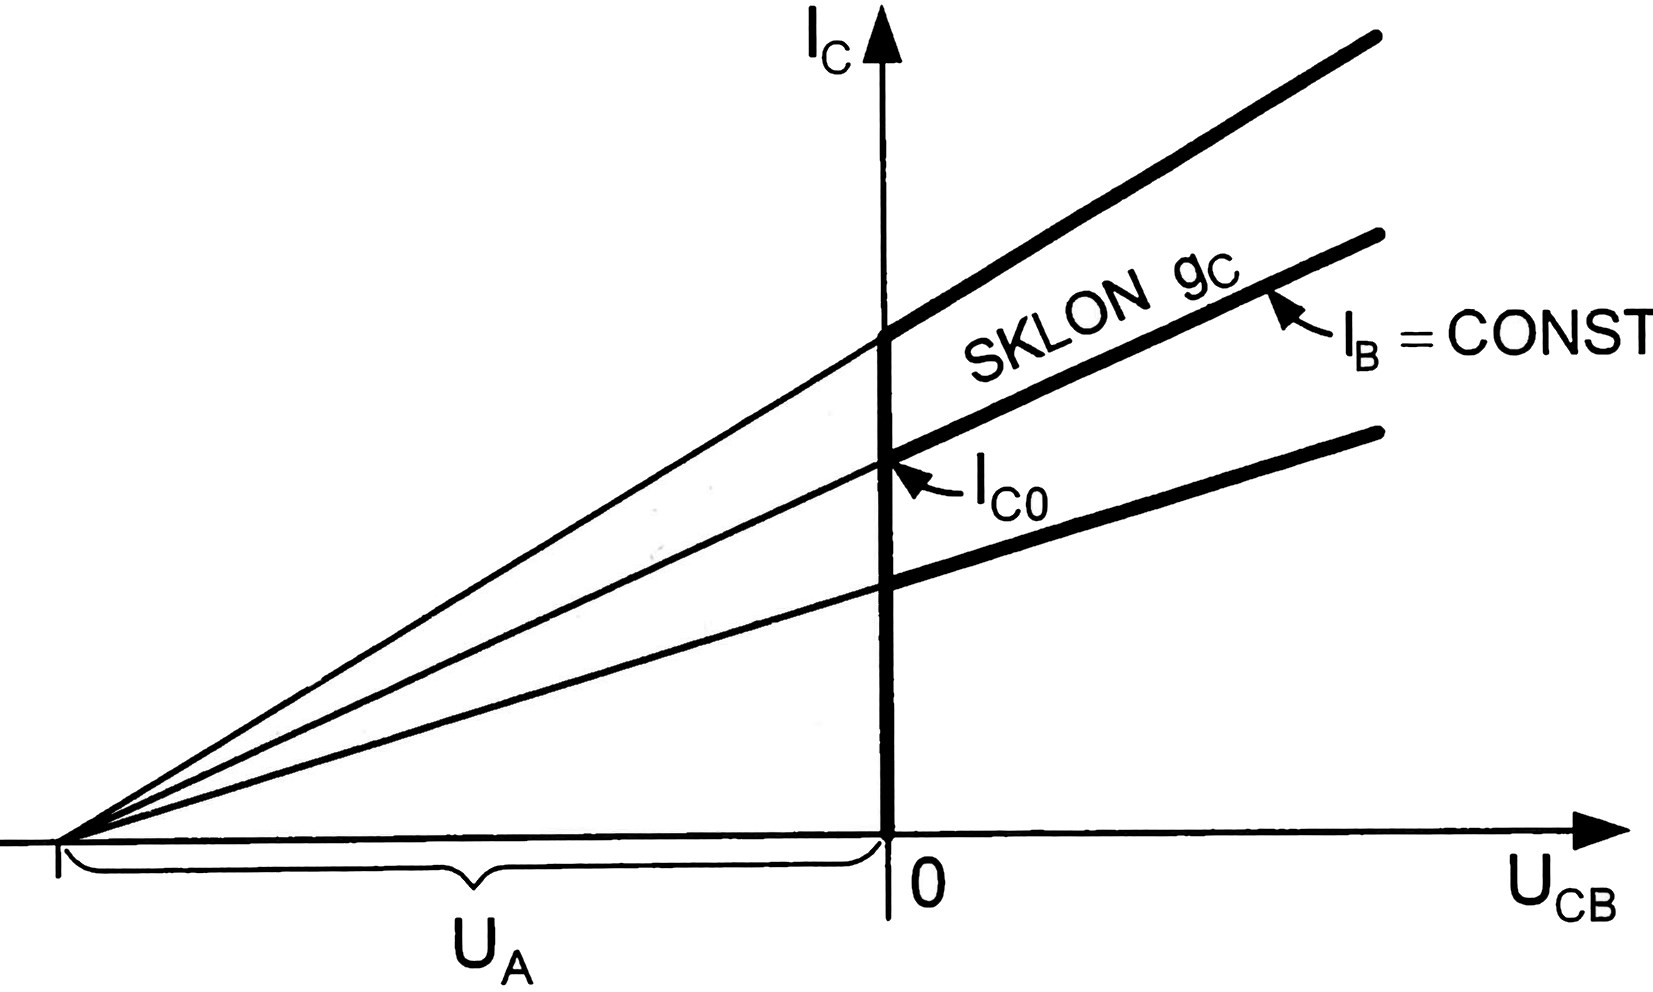
\includegraphics[width=0.6\linewidth]{aes_fig065.jpg}
          \caption{Interpretace Earlyho napětí \(U_A\) v kolektorových charakteristikách
                   \(I_C(U_{CB})\). (\cite[s.~54]{Dostal})}
          \label{aes:fig065}
        \end{figure}

        Typická velikost Earlyho napětí vstupních tranzistorů operačního zesilovače je \(U_A=
        \SI{50}{\V}\). Jinak řečeno, nasycený proud \(I_S\) a proudové zesílení \(\beta\) se
        zvětšují přibližně o \SI{2}{\percent} z výchozí hodnoty \(I_{S0}\) nebo \(\beta_0\) na každý
        \SI{1}{\V} kolektorového napětí \(U_{CB}\). Výrobní rozptyl Earlyho napětí je typicky
        \SI{50}{\percent} v souboru nevybíraných tranzistorů téhož technologického typu a
        \SI{10}{\percent} až \SI{0.1}{\percent} mezi dvěma tranzistory monolitické dvojice.

    \subsection{Unipolární vstupní stupeň}\label{aesIchIIIsecIIIssecII}
    \subsection{Konstrukční úpravy vstupního stupně}\label{aesIchIIIsecIIIssecIII}
    \subsection{Výstupní stupeň}\label{aesIchIIIsecIIIssecIV}
    \subsection{frekvenční kompenzace}\label{aesIchIIIsecIIIssecV}

%---------------------------------------------------------------------------------------------------  
  % % !TeX spellcheck = cs_CZ
%---------------------------------------------------------------------------------------------------
% file opamp.tex
%---------------------------------------------------------------------------------------------------
%================================ Kapitola: Zesilovače==============================================
\setchaptertoc
\chapter{Operační obvod}\label{aesIchIV}    
  \section{Ideální operační obvod}\label{aesIchIVsecI}
    \subsection{Paralelní operační obvod}
      \fbox{Napěťový invertor} ukazuje, že vstupní signálový proud může být generován také 
      synteticky, kombinací napěťového signálového zdroje a sériového rezistoru. Takovým způsobem 
      vytvořený \emph{napěťový invertor} na obr. * je jedním z nejčastějších operačních obvodů. 
      
      Vstupní napětí $u_s$ je celé vloženo na rezistor $R_1$ (jeho pravý konec je virtuálně 
      uzemněn) a vyvolává ekvivalentní vstupní proud $\frac{u_s}{R_1}$. Tento přitékající proud je 
      kompenzován proudem $-\frac{u_0}{R_2}$ odsávaným přes zpětnovazební rezistor $R_2$ do výstupu 
      operačního zesilovače $$\frac{u_s}{R_1}=-\frac{u_0}{R_2}.$$ Ideální operační rovnice
      \begin{equation}\label{AES:eq_opamp_inv02}
        u_0 = - \frac{R_2}{R_1}u_s.
      \end{equation}
      Vyjadřuje úměrnost signálových napětí $-u_0$ a $u_s$ velikostem přilehlých rezistorů $R_2$ a 
      $R_1$. Pro snadnější zapamatování se nabízí představa dvouramenné páky s délkami ramen $R_1$ 
      a $R_2$, otočné v bodě odpovídajícímu virtuální zemi, která přenáší výchylku $u_s$ levého 
      konce na výchylku $u_0$ pravého konce v opačné polaritě.

      \begin{figure}[ht!]
        \centering
        \subcaptionbox{$u_0 = -\dfrac{R_2}{R_1}u_s, \qquad R_{\parallel} = R_1, 
                  \qquad R_{\mathsf{O}\lvert} = s0$       \label{aes:fig075a}}
          {\luafigure[0.49]{opamp_inv01a.pdf}}                                    \newline
        \subcaptionbox{ $u_0 = -\dfrac{R_2}{R_2+R_s}u_s$  \label{aes:fig075b}}
          {\luafigure[0.50]{opamp_inv01b.pdf}}             
        \caption{Napěťový invertor. Jeho mechanickou analogií je dvouramenná páka (a). Přítomnost 
                 vnitřního odporu signálového zdroje $R_s$ v operační rovnici je důsledkem 
                 konečného vstupního odporu $R_{\parallel} = R_1$ (b). }
        \label{aes:fig075}
      \end{figure}
      Zesílení napěťového invertoru 
      \begin{equation}\label{AES:eq_opamp_inv01}
        G_i = -\frac{R_2}{R_1},
      \end{equation} 
      je záporné a nastavitelné v širokých mezích od $0$ do $\infty$ výběrem rezistorů $R_1$ a 
      $R_2$. Zvláštním případem je jednotkový invertor se stejnými rezistory $R_1 = R_2$, který 
      prostě invertuje polaritu vstupního napětí: $$u_0 = - u_s, \qquad G_i = -1.$$
      
      Výstupní odpor napěťového invertoru je ideálně nulový. Jeho vstupní odpor však ztrácí onen 
      vyhranění charakter typický pro kanonické operační obvody a nabývá indiferentní velikosti 
      \begin{equation}\label{AES:eq_opamp_inv03}
        R_{\parallel} = R_1,
      \end{equation} 
      rovné velikosti virtuálně uzemněného rezistoru $R_1$.
      
      Napěťový invertor zatěžuje signálový zdroj (obr. *). To se projevuje poklesem svorkového 
      napětí signálového zdroje o úbytek na vnitřním odporu $R_s$, nebo jinak řečeno, přítomností 
      nedefinovaného a nestálého vnitřního odporu $R_s$ v operační rovnici invertoru:  
      \begin{equation}\label{AES:eq_opamp_inv04}
       u_0 = -\frac{R_2}{R_1 + R_s}u_s.
      \end{equation}      
      Taková vlastnost se obvykle považuje za nedostatek. 
            
    \subsection{Sériový operační obvod}
    
    \subsection{Složený operační obvod}
      Operační obvody, které není možné zahrnout do předcházejích dvou velkých tříd, se vyznačují:
        \begin{itemize}[noitemsep]
          \item signálovým buzením obou vstupů operačního zesilovače,
          \item násobnou zpětnou vazbou,
          \item kombinací záporné a kladné zpětné vazby,
          \item použitím několika operačních zesilovačů,
          \item nestandardním zapojením operačního zesilovače.
        \end{itemize}
      \subsubsection{Signálové buzení obou vstupů}
        \fbox{Rozdílový zesilovač} na obr. \ref{AES:fig_diff_opamp01} je lineární operační obvod se
        dvěma vstupy. Jeho výstupní napětí se najde superpozicí \cite[s.~126]{Dostal}. 
        
        Nechť působí napětí $u_1$ a napětí $u_2$ je nulové. Neinvertující vstup operačního 
        zesilovače je uzemněn přes paralelní kombinaci rezistorů $R_3$ a $R_4$. Operační obvod 
        představuje napěťový invertor a první složka výstupního napětí má velikost 
        $$-\frac{R_2}{R_1}u_1.$$
        
        Nechť působí napětí $u_2$ a napětí $u_1$ je nulové. Operační obvod představuje neinvertujcí 
        zesilovač s předřazeným děličem $R_3$ a $R_4$ a druhá složka výstupního napětí má velikost 
        $$u_2\frac{R_4}{R_3+R_4}\left(\frac{R_2}{R_1}+1\right)= 
        u_2\frac{R_2/R_1+1}{R_4/R_3+1}\cdot\frac{R_4}{R_3}.$$
        
        %------------------------------
        % image: rozdílový zesilovač
        \begin{figure}[ht!]
          \centering
          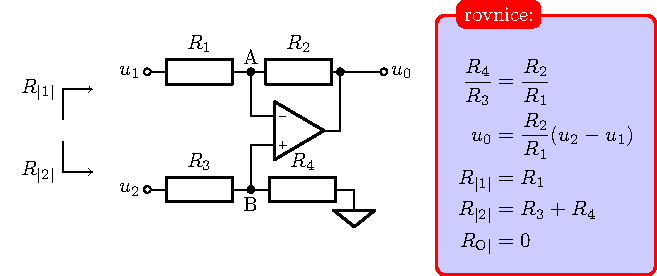
\includegraphics[width=\linewidth]{diff_opamp01.pdf}
          \caption{Rozdílový zesilovač. Podmínky potlačení souhlasné složky vstupních napětí $u_1$ a 
            $u_2$ je poměrové vyvážení zpětnovazebních rezistorů, $R_4/R_3 = R_2/R_1$. S ohledem na 
            ofset se obvykle volí uplná symetrie, tj. $R_4 = R_2$ a $R_3 = R_1$.}
          \label{AES:fig_diff_opamp01}
        \end{figure}

        Současné působení obou vstupních napětí ve vyváženém operačním obvodě
        $$\frac{R_4}{R_3}=\frac{R_2}{R_1},$$ přísluší výstupní napětí 
        \begin{equation}\label{AES:eq_diff_opamp}
          u_2 = \frac{R_2}{R_1}(u_2-u_1),   
        \end{equation}
        úměrné rozdílu vstupních napětí bez ohledu na jejich absolutní velikost. Odtud název 
        operačního obvodu. Důvod zařazení napěťového děliče ($R_3$,$R_4$) je zřejmý - dělič 
        sjednocuje zesílení invertujícího a neinvertujícího vstupu, která se liší absolutně o 
        jednotku. 
        
        Dvěma vstupům přísluší dva vstupní odpory. První vstupní odpor
        $$R_{\abs{1}} = R_1$$ je roven velikosti rezistoru $R_1$, protože vnitřní odpor bodu
        $A$\footnote{obdoba virtuální země} je nulový. Druhý vstupní odpor $$R_{\abs{2}} = R_3 +
        R_4$$ je roven součtu rezistorů $R_3$ a $R_4$, protože vnitřní odpor zbytku operačního
        obvodu v bodě $B$ je nekonečný. Tyto dva vstupní odpory jsou různé, i když jsou obě větve
        ($R_1$, $R_2$) a ($R_3$, $R_4$) stejné. 
        
        Vstupní odpory $R_{\abs{1}}$ a $R_{\abs{2}}$ přísluší dvěma samostatným uzemněným zdrojům 
        signálových napětí $u_1$ a $u_2$ podle \ref{AES:fig_diff_opamp01}. Volnému (izolovanému) 
        signálovému napěťovému zdroji připojenému diferenčně mezi vstupy rozdílového zesilovače, by 
        příslušel diferenční vstupní odpor $$R_{\abs{D}} = R_1 + R_3,$$ rovný součtové velikosti 
        rezistorů $R_{\abs{1}}$ a $R_{\abs{3}}$, protože body $A$ a $B$ jsou virtuálně zkratovány.

  \section{Analýza reálného operačního obvodu}\label{aesIchIVsecII}
  \section{Statické a dynamické chyby ve frekvenční oblasti}\label{aesIchIVsecIII}
  \section{Dynamické chyby v časové oblasti}\label{aesIchIVsecIV}
  \section{Vstupní a výstupní impedance}\label{aesIchIVsecV}
  \section{Ofset}\label{aesIchIVsecVI}
  \section{Šum}\label{aesIchIVsecVII}
  \section{Stabilita}\label{aesIchIVsecVIII}
%---------------------------------------------------------------------------------------------------
  
  % % !TeX spellcheck = cs_CZ
%---------------------------------------------------------------------------------------------------
% file opamp.tex
%---------------------------------------------------------------------------------------------------
%================================ Kapitola: Zesilovače==============================================
\setchaptertoc
\chapter{Napěťové komparátory}\label{aesIchV}  
  
  Komparátor je podobný operačnímu zesilovači. Má dva vstupy (invertující, neinvertující) a jeden
  výstup (viz \ref{aes:fig066}). Je však speciálně navržen pro porovnání napětí mezi oběma vstupy.
  Komparátor pracuje s otevřenou smyčkou a poskytuje dvoustavové logické výstupní napětí. Tyto dva
  stavy odpovídají znaménku rozdílu\footnote{včetně účinků vstupního ofsetového napětí komparátoru}
  mezi oběma vstupy.
  
  Na výstupu komparátoru bude vysoká úroveň napětí, pokud vstupní signál na neinvertujícím vstup
  převyšuje signál na invertujícím vstupu (plus ofsetové napětí, \(V_{os}\)) a nízkou úroveň pro
  opačný případ. Z hlediska terminologie používané v oblasti logických obvodů nabývá komparátor
  logickou "\texttt{1}" nebo "\texttt{0}", případně \texttt{H} (high) nebo \texttt{L} (low).
  
  Komparátor je běžně používán v aplikacích, kde je nějaká proměnná úroveň signálu porovnána s
  pevnou úrovní (obvykle referenční napětí). Protože je to ve skutečnosti \emph{1-bitový}
  analogově-digitální převodník (ADC), je komparátor základním prvkem ve všech ADC.
  (\cite[s.~72]{Vrba2000} a \cite[s.~2]{MT083}).

  \luagraphic[1]{aes_fig066.png}{Napěťový komparátor \cite[s.~1]{MT083}}{aes:fig066}

  \section{Funkce komparátoru}\label{aesIchVsecI}
    Zapojíme-li operační zesilovač podle obr. \ref{aes:fig067a}, potom se bude projevovat jeho velké
    zesílení. Je-li napájecí napětí zesilovače \SI{15}{\volt}, potom můžeme předpokládat, že
    maximální rozkmit výstupního signálu bude asi \SI{13.5}{\volt}. Meze, mezi kterými se může
    výstupní signál pohybovat jsou na převodní charakteristice uvedené na obr. \ref{aes:fig067b}
    označeny \(U_{sat}\) a \(-U_{sat}\). Velmi velká hodnota zesílení otevřené smyčky \(A_{os}\)
    činí operační zesilovač velmi citlivý na velikost rozdílu vstupních signálů.

    \begin{figure}[ht!]  %\ref{aes:fig067}
      \centering
      \subcaptionbox{\label{aes:fig067a}}{\luafigure[0.9]{aes_fig067a.png}} \\    
      \subcaptionbox{\label{aes:fig067b}}{\luafigure[0.9]{aes_fig067b.png}}                                             
      \caption{a) Zapojení operačního zesilovače bez obvodu zpětné vazby, b) převodní
              charakteristika operačního zesilovače (\cite[s.~177]{Dolecek2007})}
      \label{aes:fig067}
    \end{figure}

    Na charakteristice na obr. \ref{aes:fig067b} jsou uvedené meze výstupního signálu dosaženy již
    při velmi malých hodnotách diferenčního napětí ud na vstupu zesilovače (v příkladu uvedeném na
    obr. \ref{aes:fig067b} je výstup zesilovače v saturaci při rozdílu vstup ních napětí \(U_d =
    u_2 - u_1 = \SI{67.5}{\micro\volt}\).

    Prakticky můžeme říci, že když je \(u_2 > u_1\). bude mít napětí na výstupu zesilovače velikost
    \(U_{sat}\), když \(u_1 > u_2\), bude mít výstupní napětí velikost \(-U_{sat}\).

    \begin{tcnote}
      Doba přepnutí výstupního napětí OZ z jedné meze na druhou je omezena rychlostí přeběhu
      použitého zesilovače.
    \end{tcnote}

    Napěťový komparátor je, stejně jako operační zesilovač, \textbf{diferenční zesilovač} s velmi
    vysokým zesílením, jehož výstup nabývá pouze dva stavy. K výstupům komparátorů je možné připojit
    různá zařízení včetně různých typů logických obvodů. Z toho důvodu mají různé komparátory různá
    zapojení výstupních obvodů. Nebudeme-li uvažovat velikosti výstupních napětí a rychlosti
    spínání, můžeme uvést dvě základní zapojení výstupních obvodů:
    \begin{itemize}[noitemsep]
      \item zapojení typu \textbf{otevřený kolektor} - označení OC \emph{(open collector)};
      \item dvojčinné zapojení s \textbf{komplementárními tranzistory} - \emph{(push-pull)}.
    \end{itemize}

    \begin{figure}[ht!]  %\ref{aes:fig068}
      \centering
      \subcaptionbox{\label{aes:fig068a}}{\luafigure[0.5]{aes_fig068a.png}} \\    
      \subcaptionbox{\label{aes:fig068b}}{\luafigure[0.6]{aes_fig068b.png}} \\
      \subcaptionbox{\label{aes:fig068c}}{\luafigure[0.6]{aes_fig068c.png}}
      \caption{a) Znázornění výstupu komparátoru s otevřeným kolektorem, c) sepnutí tranzistoru, 
              když  \(u_1 > u_2\), c) tranzistor je rozepnut, když \(u_2 > u_1\) 
              (\cite[s.~177]{Dolecek2007})}
      \label{aes:fig068}
    \end{figure}

  \section{OZ ve funkci komparátoru}
    OZ jsou určeny k přesnému zesilování signálů s vysokou linearitou a stabilitou, samozřejmostí u
    nich je \emph{záporná zpětná vazba}.
    
    Stejně jako OZ se komparátory vyznačují malou vstupní napěťovou nesymetrií, velkým zesílením
    diferenčního signálu a velkým potlačením souhlasného napětí. Hlavní rozdíly mezi nimi
    spočívají v tom, že:
    \begin{itemize}[noitemsep]
      \item komparátor má logický výstup, který po překlopení do jedné ze dvou logických úrovní
            (log 1 nebo log 0) vyjadřuje, které ze dvou vstupních napětí je větší, přechod z jedné
            do druhé úrovně je velmi rychlý, ideálně skokový;
      \item OZč má analogový výstup, jeho výstupní napětí zpravidla nedosahuje mezí daných
            velikostmi napájecích napětí;
      \item OZ jsou konstruovány pro aplikace se zápornou zpětnou vazbou, nemělo by dojít k jejich
            přebuzení, které způsobí saturaci tranzistorů.
    \end{itemize}

    Komparátory jsou většinou rychlé, některé OZ rovněž. Komparátory jsou konstruovány pro velké
    vstupní diferenční signály, zatímco záporná zpětná vazba u OZ velikost diferenčních signálů
    minimalizuje. Když je OZ přebuzený, někdy i o několik \si{\mV}, některé tranzistory ve vnitřních
    zesilovacích stupních se mohou dostat do saturace. Doba zotavení nutná k přechodu ze saturace
    může trvat relativně dlouhou dobu a zesilovač je potom mnohem pomalejší než tehdy, kdy k
    saturaci nedošlo (\ref{aes:fig070}).

    \luagraphic[1]{aes_fig070.pdf}{Doba desaturace přebuzeného OZ bývá podstatně delší než jeho
                normální skupinové zpoždění (efektivně doba průchodu signálu ze vstupu na výstup)
                a často závisí na úrovni přebuzení (\emph{overdrive}).
                \cite[s.~2]{AN849}}{aes:fig070}

    \begin{tcnote}    
      Protože pouze malá skupina OZ na trhu mají uvedenou dobu zotavení pro různé úrovně přebuzení,
      je pro uživatele nezbytné stanovit tuto dobu experimentem.  Naměřené zpoždění bude záviset na
      úrovní přebuzení v dané aplikaci. Hodnota použitá při výpočtech, by měla být nejméně dvakrát
      větší než nejhorší hodnota pozorovaná testech, protože testované vzorky nemusí být
      reprezentativním vzorkem.
    \end{tcnote} 
    
    \luagraphic[0.5]{aes_fig071.pdf}{Stejná napájecí napětí umožňuje přímé buzení logického obvodu
                výstupem OZ. \cite[s.~2]{AN849}}{aes:fig071}

    Moderní OZ často mají výstupy typu rail to rail. Jejich největší kladná hodnota výstupního
    napětí se blíží k velikosti kladné hodnoty napájecího napětí, záporná hodnota se blíží k
    velikosti záporné hodnoty napájecího napětí. Když OZ a logické obvody mají stejná napájecí
    napětí, např. +\SI{5}{\volt}, je možné z výstupů OZ přímo budit následující logické obvody
    \ref{aes:fig071}. V opačném případě je nutné mezi výstupem OZ a vstupem logického obvodu vložit
    přizpůsobovací člen \cite[s.~2]{AN849} jak je tomu na obrázku \ref{aes:fig069}.
    

    \begin{figure}[ht!]  %\ref{aes:fig069}
      \centering
        \subcaptionbox{\label{aes:fig069a}}{\luafigure[0.5]{aes_fig069a.pdf}}  
        \subcaptionbox{\label{aes:fig069b}}{\luafigure[0.5]{aes_fig069b.pdf}} \\
        \subcaptionbox{\label{aes:fig069c}}{\luafigure[0.6]{aes_fig069c.pdf}}
      \caption{Přizpůsobení výstupu OZ ke vstupu logického obvodu: a) NPN, c) MOSFET N-channel, c)
                Complementary MOS inverter (\cite[s.~2]{AN849})}
      \label{aes:fig069}
    \end{figure}

    Nejjednodušší obvody rozhraní jsou \textbf{invertory}. Mohou být postaveny s NPN tranzistory,
    avšak za cenu vyšší spotřeby dané proudem báze, nebo výhodněji MOSFET s kanálem typu N.
    vytvořeny invertory s tranzistory NPN, případné s tranzistory MOSFET s kanálem typu N. 
    
    Rezistor \(R_B\) na obr. \ref{aes:fig069a} slouží k nastavení proudu báze, rezistor \(R_L\) k
    nastavení kolektorového proudu a je-li tranzistor uzavřen, zabezpečuje vstupní proud logického
    členu ve stavu log 1. Čím menší jsou velikosti odporů, tím rychlejší je činnost zapojení. NMOS
    tranzistor na obr. \ref{aes:fig069b} by měl mít malé prahové napětí \(V_{GS(th)}
    <\SI{2}{\volt}\) a také průrazné napětí hradla \(V_{GS_{max}}\) musí být větší než \(V_A\).
    Obecně musí platit, že napájecí napětí OZ \(+V_A > +V_L\) a zároveň \(-V_A < -V_L\).

    Invertor vytvořený pomocí komplementárních tranzistorů MOSFET je znázorněn na obr.
    \ref{aes:fig068c}. Jeho výhodou je malý klidový proud. Nevýhoda spočívá ve vzniku proudových
    špiček v časovém intervalu přepínání tranzistorů, kdy jsou oba tranzis tory krátkou dobu
    současně otevřeny.

    \section{Komparační úroveň a hystereze}
      \subsection{Komparační úroveň}
        
    \section{Shrnutí}
      \begin{itemize}[noitemsep]
        \item Operační zesilovač může být použit s velkou přesností jako komparátor na nízkých
              kmitočtech\footnote{Nemá smysl použít operační zesilovač jako komparátor, pokud je
              důležitá vysoká rychlost.}. Použití přesných OZ je důležité hlavně pn porovnávání
              signálů na úrovni mikrovoltů.
        \item Použití OZ může být výhodné též z cenových důvodů, když využíváme např. tři operační
              zesilovače ze čtyř umístěných v jednom pouzdru. Použití čtvrtého zesilovače jako
              komparátoru potom může být velmi ekonomické. 
        \item Pro jejich použití jako komparátorů je nutné znát rozdíly a podobnosti mezi
              komparátory a OZ, podrobně se seznámit s jejich vlastnostmi z technické dokumentace
              a to hlavně s jejich dobami zotavení, rychlostmi přeběhu, spotřebou a cenou.
        \item Komparátory jsou určeny pro rychlé rychlé spínání a v důsledku toho často mají horší
              DC parametry než mnoho operačních zesilovačů. Proto může být vhodné použít operační
              zesilovač jako komparátor v aplikacích vyžadující nízký \(V_{OS}\), nízký \(I_B\) a
              široký \(CMR\).
      \end{itemize}        

  
  \section{Aplikace}  


%---------------------------------------------------------------------------------------------------

  % !TeX spellcheck = cs_CZ
%---------------------------------------------------------------------------------------------------
% file spice.tex
%---------------------------------------------------------------------------------------------------
%================================= Kapitola: Osciloskopy a jejich použití ==========================
\setchaptertoc
\chapter{Osciloskopy a jejich použití}

  \section{Analogové osciloskopy}
  \section{Vzorkovací osciloskopy}
  \section{Digitální paměťové osciloskopy}
   

  \section{Pasivní sondy}

    \begin{figure}[ht!]
      \centering
      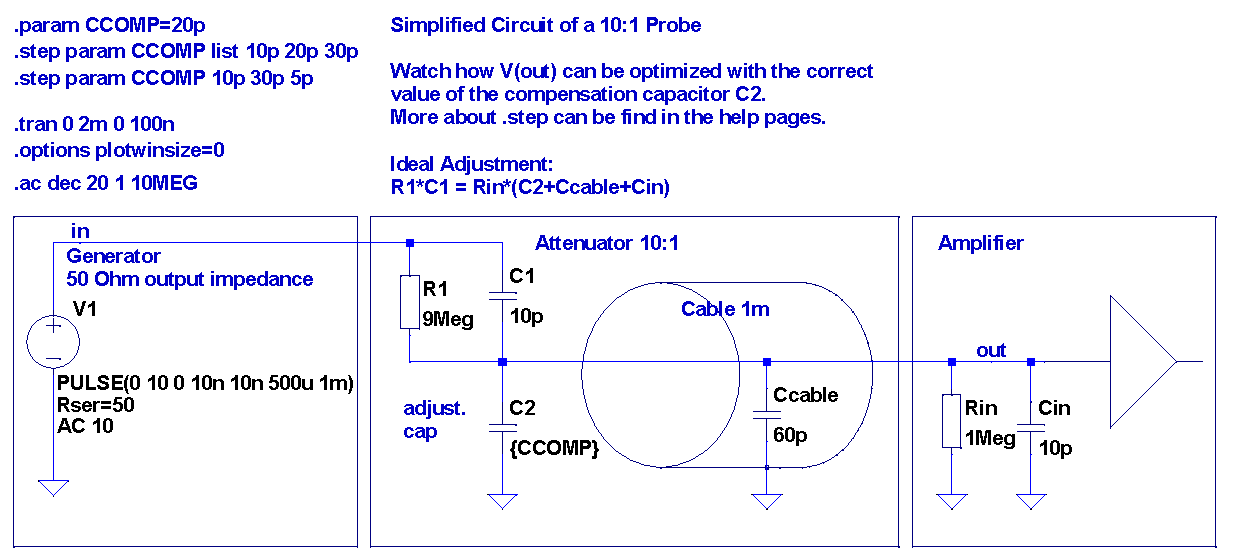
\includegraphics[width=1\linewidth]{../ltspice/ltc003_OSC_Probe_simple.pdf}
      \caption{\texttt{ltc002\_OSC\_Probe.asc}: }
      \label{SPICE:fig_ltc003_OSC}
    \end{figure}
    
    \begin{sidewaysfigure*}[ht!]
      \centering
      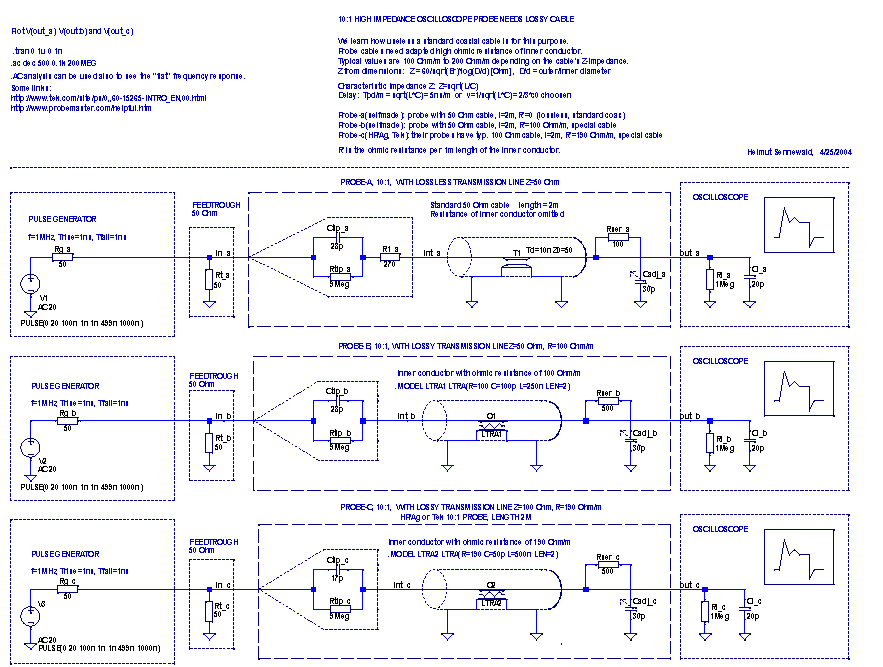
\includegraphics[width=1\linewidth]{../ltspice/ltc002_OSC_Probe.pdf}
      \caption{\texttt{ltc003\_OSC\_Probe\_simple.asc}: }
      \label{SPICE:fig_ltc002_OSC}
    \end{sidewaysfigure*}

  % \section{Aktivní sondy a proudové sondy}
  % \section{Stejnosměrná a střídavá vazba, odezva osciloskopu}
  % \section{Měření v koaxiálních obvodech}
  % \section{Časová refletometrie}
  % \section{Zobrazení XY}
  % \section{Kalibrace}
    

%--------------------------------------------------------------------------------------------------- 
}
{
% DEBUG was off
%=============== Kapitola: Modelování, analýza a simulace elektronických obvodů ===================
  % !TeX spellcheck = cs_CZ
%---------------------------------------------------------------------------------------------------
% file spice.tex
%---------------------------------------------------------------------------------------------------
%================================= Kapitola: Počítačová simulace v elektrotechnice==================
\setchaptertoc
\chapter{Modelování a simulace pomocí SPICE}

  \section{Využití počítače pro návrh obvodů}
    \subsection{Obecný návrhový proces}
      Vývoj nástrojů pro počítačové řešení elektronických obvodů je úzce spojen s vývojem výpočetní
      techniky. Již v průběhu padesátých let minulého století se objevily první programy pro řešení
      velmi specializovaných úloh. Záhy bylo zřejmé, že simulace elektronických obvodů přinese jak
      technické, tak i ekonomické výhody. 
      
      \textbf{Simulací} rozumíme proces, kdy na základě řešení rovnic matematického modelu obvodu
      získáme (přibližnou) informaci o jeho parametrech a charakteristikách. To umožňuje „přeskočit"
      řadu pokusných realizací. Např. v oblasti návrhu integrovaných obvodů je taková realizace
      značně nákladná (stovky tisíc Kč), nemluvě o velmi problematickém měření ve vnitřních uzlech
      obvodu. Některé typy analýz, jako například určení vlivu technologického rozptylu při výrobě,
      je prakticky nemožné uskutečnit. 

      \luagraphic[0.8]{aes_fig008.png}{Obecný postup při návrhu obvodu. 
      (\cite[s.~1]{KolkaBiolek2011})}{aes:fig008}
      
      Velmi zjednodušeně je možné obvyklý proces návrhu obvodu či jakékoli jiné soustavy znázornit
      podle obr. \ref{aes:fig008}. Nazývá se návrh (syntéza) metodou opakované analýzy. Blok č. 1
      představuje oblast s dominantním podílem člověka-návrháře. I přes dflčí pokroky v oblasti
      automatizované syntézy je nepravděpodobné, že bude tuto fázi možné někdy realizovat pouze
      počítačem. To platí zejména pro analogové obvody.

      Celý proces začíná „ručním“ návrhem, kdy na základě požadované funkce a za použití
      jednoduchých vztahů, při zanedbání parazitních jevů, určíme zapojení a přibližné hodnoty
      parametrů obvodových prvků. 
      
      V následujícím kroku je obvod počítačově analyzován za použití mnohem přesnějších modelů,
      které umožní postihnout i všechny významné parazitní jevy. V případě odhalení nesouladu se
      musí provést modifikace navrženého obvodu. Samozřejmě že nedílnou součástí celého procesu musí
      být ověření vlastností navržené soustavy pomocí realizace funkčního vzorku. Snahou je
      minimalizovat počet iterací této vnější smyčky, což vždy přináší úsporu nákladů na vývoj.
      Snaha navrhnout obvod tak, že zvolíme náhodné hodnoty prvků a budeme se pouze pomocí programu
      snažit najít optimum prostřednictvím jejich rozmítání nebo krokování, obvykle k cíli nevede. 
      
      Dominantní oblastí aplikace počítačových metod je numerická analýza (blok č. 2), kdy vstupem
      programu je konkrétní obvod se známými hodnotami prvků a výsledkem jeho charakteristiky. V
      dnešní době, při řešení praktických problémů za použití přesných (a složitých) modelů, není
      možné analýzu provádět ručně nebo graficky. Z hlediska vlastního návrhu plní počítačové
      programy spíše podpůrnou funkci. Výjimku představují programy pro automatizovaná řešení
      některých dílčích úloh, jako je např. návrh analogových kmitočtových filtrů nebo napájecích
      zdrojů.

    \subsection{Programy třídy SPICE}
      V roce 1971 vytvořil student „University of California“, Berkeley, USA \emph{Larry Nagel}
      program \texttt{SPICE1} (\texttt{SPICE} = \emph{Simulation Program with Integrated Circuit
      Emphasis}) v jazyku Fortran. Program umožňoval analýzu dějů v obvodech, obsahujících zejména
      bipolární a unipolární tranzistory. O věrohodnost výsledků bylo usilováno propracovaností
      modelů i matematických algoritmů řešení rovnic. Uživatel měl navíc  možnost
      roz\-ši\-řo\-vá\-ní sortimentu analyzovaných součástek technikou makromodelů zakládáním tzv.
      \emph{pod\-ob\-vo\-dů} (\texttt{subcircuits}) \texttt{SPICE} \cite[s.~2]{KolkaBiolek2011}. 
      
      Protože program byl v podstatě volně šiřitelný, stal se brzo standardním simulačním nástrojem
      pro elektrotechnické úlohy. Usilovně se pracovalo na jeho zdokonalování. V roce 1975 byla
      představena verze \texttt{SPICE2} s podstatně vylepšenými modely i numerickými algoritmy. Tato
      verze byla v průběhu téměř 20 let postupně zdokonalována na Berkeleyské univerzitě až do dnes
      všeobecně známého standardu \texttt{SPICE2G.6}, který byl v r. 1983 zpřístupněn k volnému
      používání. Zdrojové texty \texttt{SPICE1} a \texttt{SPICE2} byly napsány ve Fortranu. Vzhledem
      k zvýšenému využívání unixových pracovních stanic padlo v Berkeley rozhodnutí přepsat SPICE2
      do jazyka C. Tak začala vznikat verze \texttt{SPICE3}. Dnes je rozšířena verze
      \texttt{SPICE3F.5}. Oproti SPICE2G.6 se vyznačuje řadou vylepšení, ovšem z různých důvodů
      došlo k ztrátě zpětné kompatibility se SPICE2G.6. \cite[s.~2]{KolkaBiolek2011}

      S růstem výkonnosti počítačů PC byly programy, dosud běžící na výkonných pracovních stanicích,
      přepisovány na programy spustitelné na „PCčkách“. Tak vznikl standard \texttt{PSpice} (\emph{P
      = počítače PC}). Dnes existuje více simulačních programů, které využívají v podstatě tři ne
      zcela kompatibilní standardy: \texttt{SPICE2}, \texttt{SPICE3}, \texttt{PSPICE}. 
      
      Z hlediska uživatele se mírná odlišnost v syntaxi vstupních souborů projeví zejména při práci
      s modely. Výrobci elektronických prvků obvykle publikují modely ve tvaru \texttt{SPICE2}, aby
      pracovaly ve většině simulátorů. Tím se ovšem nevyužívají možnosti novějších programů. Pokud
      je model napsán ve vyšší verzi, nastávají problémy s nekompatibilitou a text modelu je nutné
      modifikovat.
      
      Z tohoto důvodu se simulátory rozdělují na tzv. „\emph{Spice-like}“ a „\emph{Spice-compatible}
      “simulátory. Označení „\emph{Spice-like}“ znamená, že simulátor je schopen generovat podobné
      výsledky analýzy jako \texttt{SPICE}, avšak nemusí být schopen číst standardní vstupní soubory
      SPICE. Typickými příklady jsou staré verze programů \texttt{Micro-Cap} nebo \texttt{TINA},
      program apod. Termínem „\emph{Spice-compatible}“ se označují simulační programy, které dokáží
      číst standardní vstupní soubory \texttt{SPICE}, provádět klasické \texttt{SPICE} analýzy, a
      generovat výsledky v standardním \texttt{SPICE2G.6} tvaru. Ze současných programů jsou to
      například \texttt{PSpice}, \texttt{HSpice} (standard SPICE3), \texttt{WINSpice} (standard
      \texttt{SPICE3}), \texttt{MicroCap} od verze IV, \texttt{Multisim}, \texttt{LTspice} (standard
      \texttt{SPICE3}) a další.

      Kromě toho existují programy pro simulaci obvodů, které nemají s výše uvedenými skupinami
      programů mnoho společného. Jedná se zejména o jednoúčelové programy, specializované na analýzy
      obvodů, které nelze realizovat programy typu \texttt{SPICE}. Programy typu
      „\texttt{SPICE-compatible}“ jsou široce využívány mimo jiné proto, že umožňují neomezené
      rozšiřování sortimentu modelovaných součástek o nové typy, jejichž modely se průběžně objevují
      na webu a následně i v inovovaných knihovnách nových verzí programů. Na akademických
      pracovištích i v průmyslu je oblíbeným produktem OrcadPSpice. \cite[s.~10]{Biolek2005}

      Programy třídy \texttt{SPICE} umožňují tři základní typy analýz. Každá analýza odpovídá
      jistému laboratornímu experimentu, kdy za pomocí signálních generátorů a měřicích přístrojů
      zkoumáme daný obvod. 
      \begin{enumerate}[leftmargin=1cm,rightmargin=.1cm, label=\emph{\alph*}),noitemsep]
        \item \textbf{Analýza v časové oblasti, též přechodová - Transient}: Jedná se o analýzu, kdy
              výsledkem jsou časové průběhy napětí, proudů a z nich odvozených veličin v obvodu.
              Odpovídá laboratornímu experimentu, kdy chování obvodu sledujeme pomocí osciloskopu.
              Kromě napájecích zdrojů mohou být ve schématu i příslušné signální generátory (tj.
              nezávislé zdroje napětí a proudu). 
        \item \textbf{Stejnosměrná analýza - DC}: Předpokládá se, že napětí a proudy se v čase
              nemění, resp. mění tak pomalu, že je můžeme považovat za „stejnosměrné“. Výsledkem
              analýzy je závislost (stejnosměrných) napětí a proudů na nějakém parametru - vstupním
              napětí/proudu, velikosti odporu rezistoru, teplotě, atd. 
        \item \textbf{Střídavá analýza - AC}: Na vstup obvodu je připojen harmonický (sinusový)
              generátor. Předpokládá se, že všechna napětí a proudy jsou harmonické, tj. v obvodu
              dochází pouze k zanedbatelnému zkreslení. Výsledkem jsou amplitudy a fázové posuny
              všech napětí a proudů (komplexní fázory) v závislosti na frekvenci signálu. Tato
              analýza umožňuje zjistit komplexní napěťové přenosy, impedance a admitance. Střídavá
              analýza je použitelná jen pro obvody, které pracují v lineárním režimu, tj.
              zesilovače, kmitočtové filtry, různé přenosové články. Střídavou analýzu nelze použít
              pro obvody, jejichž činnost je založena na využití nelinearity (směšovače, násobiče,
              usměrňovače, atd.).
      \end{enumerate}

      Ostatní analýzy využívají výsledků některé ze základních analýz. Patří k nim
      \textbf{parametrická analýza}, kdy je krokován vybraný parametr (napětí, odpor, teplota,
      atd.). Výsledkem je svazek křivek. \textbf{Citlivostní analýza} poskytuje informace o tom, jak
      změna prvku ovlivní chování obvodu. Např. u oscilátoru můžeme údajem o citlivosti v
      \si{\Hz\per\percent} stanovit, o kolik \si{\Hz} se změní kmitočet při změně parametru
      sledovaného prvku o \SI{1}{\percent}. Analýza \textbf{Monte Carlo} simuluje hromadnou výrobu
      náhodným generováním hodnot parametrů prvků. Pak je možné statisticky vyhodnotit míru
      „výrobního“rozptylu sledovaného parametru. Analýza \textbf{Worst-Case} zjišťuje nejhorší
      možnou kombinaci parametrů prvků v rámci jejich tolerančních intervalů. Obvykle se jedná o
      nadstavbu citlivostní analýzy.

      \subsection{Základní principy obvodové simulace}
        Smyslem počítačové simulace je poskytnutí adekvátní informace o modelované fyzikální
        soustavě pro ověření funkce, resp. další postup návrhu. Forma, jakou je stav obvodu popsán,
        závisí na řešeném problému. Hypoteticky by bylo možné na základě kvantové teorie sestavit
        soustavu rovnic pro pohyb elementárních částic. Z jejího řešení je pak možné odvodit všechny
        další charakteristiky. Je zřejmé, že např. pouhé vykreslení voltampérové charakteristiky
        diody by znamenalo nepřekonatelný výpočetní problém. V dnešní době, i při použití
        nejvýkonnějších počítačů, je možné takto simulovat pouze mikroskopické objekty. Matematický
        model je také možné sestavit s uvažováním např. hustoty nosičů v elementu objemu polovodiče.
        I když bude řešení méně náročné, je proveditelné pro soustavy s maximálně desítkami prvků.
        Nezajímá-li nás dění uvnitř prvku, můžeme pro modelování použít analytické vztahy pro
        svorková napětí a proudy. Pak je možné vyřešit obvody až s desítkou tisíc tranzistorů.

        \luagraphic[1]{aes_fig009.png}{Různé úrovně abstrakce při modelování číslicového obvodu. 
        (\cite[s.~3]{KolkaBiolek2011})}{aes:fig009}

        Hloubka a rozsah informace, získané o objektu, je nepřímo úměrná \emph{úrovni abstrakce}. Na
        obr. \ref{aes:fig009} je znázorněn význam tohoto pojmu. Čím je vyšší úroveň abstrakce, tím
        méně máme informací o jednotlivostech. Na druhou stranu je však možné postihnout větší
        soustavy. Např. na procesor pro stolní počítače se nikdy nedíváme jako na 25 milionů
        tranzistorů, ale jako na systém, který se skládá z bloků (ALU, řadič,...), které dále dělíme
        na registry, hradla, atd. 
        
        Předmětem našeho zájmu bude tzv. \textbf{obvodová simulace}, kdy se obvod modeluje na úrovni
        svorkových napětí a proudů jednotlivých prvků.
      
        \subsubsection{Soustava se soustředěnými parametry}
          Obvod budeme nazývat \emph{soustavou se soustředěnými parametry}, jestliže je možné jej
          rozložit na konečný počet elementárních bloků tak, aby vzájemné energetické interakce
          probíhaly výhradně v konečném počtu idealizovaných bodových svorek - uzlů. Blok může
          představovat jednotlivou součástku nebo větší podsoustavu. Takové dělení je možné
          hierarchicky opakovat.

          \luagraphic[1]{aes_fig010.png}{Rozklad obvodu se soustředěnými parametry. 
          (\cite[s.~3]{KolkaBiolek2011})}{aes:fig010}

          Na obr. \ref{aes:fig010} je znázorněn RC obvod. Ačkoli se spoje mezi prvky kreslí jako
          čáry a nazývají se vodiči, tak soustava takových spojených „vodičů“ představuje uzel -
          bodový objekt, který nemá žádné parazitní vlastnosti. 
          

          Soustavu se soustředěnými parametry můžeme tedy plně popsat souborem prvků a definicí
          vzájemného propojení jejich uzlů, tj. definicí jejich interakcí. Takový popis se nazývá
          slangově netlist (termín převzatý ze simulačních programů). Pro obvod na obrázku by
          netlist standardu \texttt{SPICE} měl tvar:
          \begin{lstlisting}[gobble=8, xrightmargin=13em]
            R1 1 2 1k
            R2 2 0 1k
            C1 2 0 1n
          \end{lstlisting}

          Požadavek na to, aby energie procházela jen přes uzly, není možné fyzikálně splnit. Např.
          pro obvod na obr.\ref{aes:fig010} bude spojení mezi pasivními prvky provedeno pomocí
          plošných spojů. Při připojení střídavého buzení bude k proudům daného uzlu přispívat i
          posuvný proud jeho vlastní (parazitní) kapacity, takže součet proudů přicházejících ze
          svorek jednotlivých prvků nebude zdánlivě roven nule. Stejnou úvahu je možné učinit i o
          napětí indukovaném ve vodiči. Převažuje-li jedna složka pole (např. jen posuvný proud),
          tak je možné do původního obvodu doplnit další prvek (parazitní kapacitu), který bude
          modelovat vlastnosti fyzikálně realizovaného uzlu. Celá soustava tak opět bude mít
          charakter obvodu se soustředěnými parametry a bude plně popsána souborem prvků a definicí
          jejich propojení. Je tedy zřejmé, že pojem \emph{obvodu se soustředěnými parametry} je
          vždy aproximací reality, která nutně přináší chybu. Není-li možné s přijatelnou chybou
          takto obvod řešit, pak musíme použít metody pro \emph{systémy s rozloženými parametry}.

          \luagraphic[1]{aes_fig011.png}{Zahrnutí parazitního prvku (kapacity plošného spoje) do
          modelu obvodu. (\cite[s.~3]{KolkaBiolek2011})}{aes:fig011}

          Na obr. \ref{aes:fig011} je znázorněn proces zahrnutí parazitní kapacity spoje do modelu
          obvodu. V okamžiku návrhu můžeme parazitní vlastnosti spojů pouze odhadnout. Vyžaduje-li
          to povaha úlohy, je možné pomocí speciálního software vypočítat parazitní vlastnosti již
          navrženého např. plošného spoje za účelem provedení ověřovací simulace a eventuální
          korekce návrhu.

        \subsubsection{Modely elektronických prvků}
          \textbf{Modelem} fyzikálního objektu nazýváme reprezentaci tohoto objektu symbolickým
          popisem (rovnicemi) nebo jiným objektem („náhradním schématem“), který z hlediska zkoumaných
          vlastností nahrazuje modelovaný objekt.

          Vzhledem k výhradnímu používání počítačů je modelem elektronického prvku vždy soustava
          rovnic, které říkáme matematický model. Na úrovni obvodové simulace tyto modely popisují
          vztahy mezi svorkovými veličinami (napětí a proudy). V rovnicích vystupují různé
          koeficienty, kterým říkáme parametry modelu.

          Např. matematickým modelem rezistoru (ideálního prvku) je známý vztah
          \begin{equation*}
            u = Ri
          \end{equation*}
          Parametrem tohoto modelu je odpor \(R\).

          \textbf{Identifikací modelu} rozumíme postup pro získání jeho matematického popisu. Velmi
          často se identifikací nazývá pouze proces získání parametrů, když je tvar rovnic předem
          znám.

          \begin{table*}
            \centering
            \begin{tabular}{|p{4cm}|p{4cm}|p{3cm}|}
              \hline
              \rowcolor{CornflowerBlue}{typ}                                & { } & {Model}   \\
              \hline
              rezistor (idealizovaný prvek)             
                & 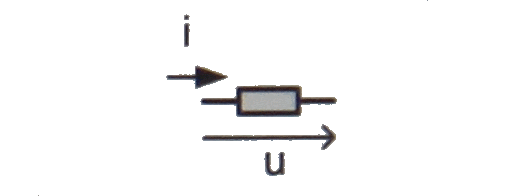
\includegraphics[width=1\linewidth]{aes_fig012a.png}      & \(u = Ri\)      \\
              \hline
              rezistor (model pro vyšší frekvence)      
                & 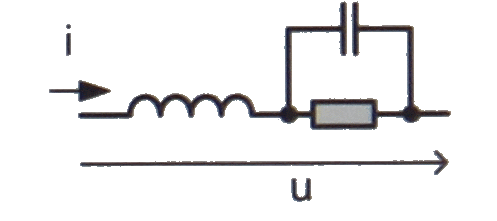
\includegraphics[width=1\linewidth]{aes_fig012b.png}      
                & náhradní schéma tvořené elementárními prvky \\ 
              \hline    
              nelineární prvek - varistor               
                & 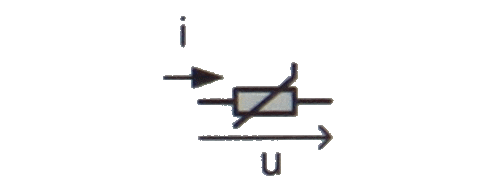
\includegraphics[width=1\linewidth]{aes_fig012c.png}      & \(i = Au^B\)    \\
              \hline
              polovodičová dioda (elementární model)    
                & 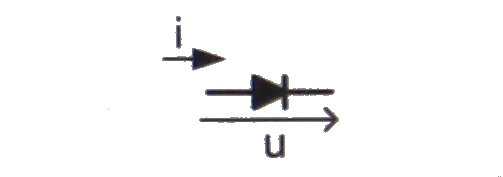
\includegraphics[width=1\linewidth]{aes_fig012d.png} 
                &  \(i = I_s\left(e^\frac{u}{nV_T}-1\right)\)  \\
              \hline 
            \end{tabular}
            \caption{Příklady modelů}\label{aes:tab001}
          \end{table*}

          Matematický model celého obvodu vznikne sloučením modelů dílčích prvků s Kirchhoffovými
          rovnicemi, které popisují interakce mezi prvky. Výsledkem je soustava tzv.
          \emph{algebraicko-diferenciálních rovnic}. Běžný uživatel simulačního programu, na rozdíl od
          jeho tvůrce, se s těmito rovnicemi přímo nesetká.

      \subsection{Simulace a realita}
        Přes všechen pokrok v oblasti počítačové podpory návrhu však dosud neexistuje program, do
        něhož by uživatel zadal obvod (schéma) a po stisknutí tlačítka obdržel důvěryhodné výsledky,
        aniž by o obvodu něco věděl. Výsledky mohou být chybné a je jen na uživateli, aby je kriticky
        posoudil. 
        
        Příčiny nesouladu mezi realitou a simulací můžeme rozdělit do čtyř kategorii:
        \begin{enumerate}[leftmargin=2cm,rightmargin=0.8cm, label=\emph{\alph*}),noitemsep]
          \item chyby vzniklé při vlastním řešení rovnic obvodového modelu v simulátoru, 
          \item nepřesné modely,
          \item výrobní rozptyl, 
          \item zanedbané parazitní prvky.
        \end{enumerate}

        \begin{itemize}[noitemsep]
          \item \textbf{Chyby simulátoru}: Při numerickém řešení soustavy rovnic, popisující obvod,
                vznikají chyby zaokrouhlováním, diskretizací i iteračním způsobem řešení.
                Pomineme-li problémy prvků popsaných ve frekvenční oblasti a tzv. špatně podmíněné
                úlohy, tak je možné říci, že přesnost výpočtu má uživatel pod kontrolou
                prostřednictvím parametrů RELTOL, ABSTOL a VNTOL (\todo[inline]{blíže v kap. 1.4.2.1}).
                Obvykle je nastavena relativní chyba \SI{0.1}{\percent}. Požadování vyšší přesnosti
                zpomalí simulaci nebo může v krajním případě vést k jejímu selhání. Je také
                diskutabilní, zdali požadovat výrazně vyšší přesnost simulace, než mohou mít měřicí
                přístroje v laboratoři. 
          \item \textbf{Nepřesné modely}: Každý model je jen aproximací reality. Používané modely
                jsou kompromisem mezi požadavkem na přesnost, výpočetní efektivitu a možnost snadné
                identifikace parametrů na základě měření.
          \item \textbf{Výrobní rozptyl}: Výrobní rozptyl je značný zejména u polovodičů. Např.
                proudový zesilovací činitel bipolárního tranzistoru může mít toleranci až
                \SI{\pm50}{\percent}.
          \item \textbf{ Odhad parazitních prvků}: Dalším problémem jsou parazitní vlastnosti
                propojovacích vodičů mezi prvky. To, co je nakresleno v editoru schématu jako vodič,
                vlastně představuje ideální spoj bez parazitní indukčnosti, odporu i kapacity.
                Zvláště při analýze obvodů v megahertzové oblasti vyžaduje odhad parazitních prvků i
                jistou zkušenost s praktickou realizací. Při neuvažování parazitních prvků vlastně
                analyzujeme neúplný model obvodu.                          
        \end{itemize}

        \begin{tcnote}
          Vliv výrobního rozptylu si ukažme na příkladu (nevhodného) nastavení pracovního body
          zesilovače v zapojení \texttt{SE}. Zapojení je velmi citlivé na parametry tranzistoru.
          Předpokládejme, že máme konkrétní kus tranzistoru \texttt{Philips/NXP BC546A}, který
          změříme a na základě změřených hodnot vytvoříme model. V tom případě bude chyba mezi
          simulací a měřením např. kolektorového proudu řádu procent.
          
          {\centering
          \captionsetup{type=figure}
            \subcaptionbox{\label{aes:fig013a}}{\luafigure[.45]{aes_fig013a.png}} 
            \hspace{1em} 
            \subcaptionbox{\label{aes:fig013b}}{\luafigure[.45]{aes_fig013b.png}}  
          \captionof{figure}{a) Nastavení pracovního bodu; b) model a skutečné prvky
                      (\cite[s.~6]{KolkaBiolek2011}) \label{aes:fig013}} \par}

        Uvažme nyní, že použijeme jiný kus téhož typu a stále stejný model. Podle údajů katalogového
        listu leží proudový zesilovací činitel \(h_{21E}(\beta)\) v rozmezí \num{110} až \num{220}.
        U druhého tranzistoru bude parametr h21e jiný, dopředu neznámý. I kdybychom vytvořili
        dokonalý model pro první tranzistor, tak při použití druhého tranzistoru dostaneme odchylku
        v řádu desítek procent.

        V praxi se navíc vytvářejí modely spíše pro typické hodnoty, které ani nemusí popisovat
        konkrétní existující kus. Na obr. \ref{aes:fig013b}  je to ilustrováno graficky (pro případ,
        kdyby měl model jen dva parametry). Je tedy zřejmé, že otázka: \uv{Jakou hodnotu bude mít
        kolektorový proud?} je nesprávně položena. Správně položená otázka zní: \uv{V jakém rozsahu
        se může nacházet kolektorový proud, když uvážíme výrobní rozptyl všech prvků?} Pak teprve
        můžeme porovnávat simulaci a realitu.

        Musíme se tedy smířit s tím, že model vždy vyjadřuje jen parametry jednoho (hypotetického)
        prvku. Dobrý model musí navíc věrně postihovat např. závislost parametrů na teplotě,
        frekvenci, nebo kolektorovém proudu.
      \end{tcnote} 

  \section{Modelování základních obvodů}
    \subsection{Typické uspořádání simulačních programů}
      Pojem \texttt{SPICE} označuje vlastní výpočetní jádro, které řeší obvodové rovnice. Moderní
      simulátory jsou obvykle součástí větších systémů pro kompletní návrh klasických nebo
      integrovaných obvodů.

      Bohužel standard \texttt{SPICE} není zaštítěn žádnou respektovanou organizací. Proto existují
      mezi jednotlivými programy drobné rozdíly v syntaxi vstupních souborů. Knihovny a vytvořené
      obvody obvykle nejsou automaticky plně přenositelné. Většinou programy zachovávají zpětnou
      kompatibilitu se syntaxí použitou ve \texttt{SPICE2} a \texttt{SPICE3}. Pokud např. výrobci
      prvků poskytují (na Internetu) modely, tak v naprosté většině právě v kompatibilní formě. To
      má za následek, že se nevyužijí možnosti, které byly přidány do různých komerčních variant
      \texttt{SPICE}.

      Na obr. \ref{aes:fig014} je ustálené uspořádání simulačního programu. Systém obvykle obsahuje
      tři moduly: \emph{editor schématu}, \emph{simulátor} a \emph{postprocesor} - modul pro
      vykreslování výsledků analýzy a jejich další zpracování. Editory schématu a postprocesory se
      od jednotlivých výrobců velmi výrazně odlišují. Z pohledu uživatele má největší význam to, že
      rozhraní editor + simulátor je víceméně standardizované. Právě tomu se říká „standard SPICE“.
      Informace o obvodu a požadovaných analýzách jsou simulátoru předávány pomocí textových
      souborů. Přenositelnost jak obvodů, tak knihoven modelů je zajištěna právě na úrovni těchto
      souborů. To je důvod, proč se všechny obvody a modely publikují jako textové soubory. Formáty
      souborů pro uložení schématu jsou většinou neveřejné, často podléhající licenci.

      \luagraphic[1]{aes_fig014.png}{Typické uspořádání simulačního programu. 
      (\cite[s.~8]{KolkaBiolek2011})}{aes:fig014}      

      Na obr. \ref{aes:fig015} je příklad organizace souborů pro stejnosměrnou analýzu jednoduchého
      obvodu s diodou, kdy napětí stejnosměrného zdroje je rozmítáno od \SI{-3}{\V} do \SI{+3}{\V}.
      Vstupní soubor je vygenerován automaticky editorem schématu nebo může být editován ručně.
      První část tvoří popis samotného obvodu. Každému prvku odpovídá jeden řádek. Parametry zdroje
      napětí (\texttt{V\_V1}) a rezistoru (\texttt{R\_R1}) jsou plně popsané v netlistu. Uzly jsou
      ve schématu očíslované jako \num{1} a \num{2}, referenční uzel je vždy \num{0}. Dioda je
      popsána složitým modelem s mnoha parametry, který je uložen v knihovně spolu s dalšími modely.
      Řádek v netlistu obsahuje jen odkaz na model.

      \luagraphic[1]{aes_fig015.png}{Struktura vstupních souborů.
      (\cite[s.~9]{KolkaBiolek2011})}{aes:fig015}      

      Jméno knihovního souboru je uvedeno v příkazu \texttt{.LIB}. V poslední části jsou příkazy pro
      rozmítání stejnosměrné složky \(V_1\) s krokem \SI{50}{\mV}. Příkaz \texttt{.PROBE} určuje, že
      napětí obou uzlů se budou ukládat pro zpracování v postprocesoru (zobrazení grafů). Model z
      knihovny (příkaz \texttt{.model...}) může být umístěný v hlavním souboru. V tom případě
      knihovnu nepotřebujeme a celá úloha je definovaná jen jedním souborem. Tento styl je výhodný,
      pokud někomu potřebujeme poskytnout náš \uv{obvod} v textové formě. Netlistem by se měl
      nazývat jen soupis prvků. Někdy se tak ovšem říká i celému vstupnímu souboru, obsahujícímu
      také příkazy.
      
      \begin{tcnote}
        Uživatel simulačního programu je prakticky vždy nucen pracovat i s textovými soubory
        knihoven nebo netlistů, například při zahrnování nového modelu do knihovny nebo hledání
        chyb podle hlášení simulátoru.
      \end{tcnote}

      Vstupní soubor z obr. \ref{aes:fig015} je možné \uv{odsimulovat} programem
      \texttt{PSpice}. Hlavní textový soubor nazveme např. jako \texttt{obvod.cir}
      a knihovnu jako \texttt{diody.lib} (text lze zkopírovat přes schránku Windows). Spustíme
      program \texttt{PSpiceAD} (nikoli editor schématu \texttt{Capture}). Zvolíme
      \texttt{File/Open} a nastavíme typ souboru na \texttt{*.cir}. Volbou \emph{Simulation/Run} se
      spustí analýza. Po skončení se pomocí \texttt{Trace/Add Trace} zobrazí např. průběh \(v(2)\) -
      napětí na diodě. \todo[inline]{Podrobnosti viz kapitola 1.2.4 na str. 20.s}

    \subsection{Základní pravidla jazyka (P)Spice}
      Kromě definice struktury obvodu a modelů prvků obsahuje vstupní soubor i příkazy pro simulátor
      k provádění různých analýz, ukládání výsledků a nastavování parametrů algoritmů pro numerické
      řešení.

      \begin{tcnote}
        Syntaktická pravidla:
        \begin{itemize}[noitemsep]
          \item První řádek vždy slouží jako hlavička (nadpis), \texttt{PSpice} jej
                ignoruje\footnote{na obr. \ref{aes:fig015} je to řádek: \texttt{* obvod}}. 
          \item Prázdné řádky, vícenásobné mezery a další „bílé znaky“ se ignorují. 
          \item Malá a velká písmena se nerozlišují. 
          \item Na pořadí řádků nezáleží (s výjimkou prvního a posledního řádku). 
          \item Názvy všech obvodových prvků musí být jedinečné. 
          \item Každý řádek (s výjimkou hlavičky) začíná jedním z těchto symbolů: 
                \begin{itemize}[noitemsep]
                  \item \textbf{znak 'A' až 'Z'} - definice obvodového prvku (např. R pro
                        rezistor\footnote{Jednotlivé verze SPICE se mohou mírně lišit v přiřazení
                        znaků k prvkům.}).
                  \item \textbf{znak '*'} - obsah řádku je chápán jako komentář. 
                  \item \textbf{znak '+'} - řádek je pokračováním předchozího řádku\footnote{Používá
                        se pro zlepšení čitelnosti.}. 
                  \item \textbf{znak '.'} - příkaz simulátoru (např. \texttt{.DC} provede
                        stejnosměrnou analýzu).
                \end{itemize}
          \item Vše, co je napravo od znaku středník ';', je chápáno jako komentář.
          \item Soubor končí příkazem \texttt{.END}. 
          \item Uzly se značí alfanumerickým řetězcem bez mezer. Původní standard dovoloval jen
                označení celými čísly. Jeden z uzlů musí být označen jako O (nula).
          \item Čísla se zapisují v přirozeném tvaru (\num{0.25}) vždy s desetinnou tečkou, v
                exponenciálním tvaru (1e-3), nebo je možné použít standardní technické přípony
                (\texttt{f, u, m, k, meg, g, t}). Mezi číslem a příponou se nesmí psát mezera.
                Ostatní znaky za číslem se ignorují (\texttt{1uF = 1u}). Přípona \texttt{m} i
                \texttt{M} znamená \texttt{mili} (\num{e-3}) - nerozlišují se malá a velká písmena. 
          \item Od \texttt{PSpice} verze 15 je možné využívat i tzv. Evropský způsob, kdy se přípona
                píše místo desetinné tečky. Např. \texttt{4k7 = 4.7k}. Místo desetinné tečky je také
                možné použít \texttt{R} pro rezistory, \texttt{L} pro induktory a \texttt{C} pro
                kapacitory. Např. \texttt{1R2 = \SI{1.2}{\ohm}}, ale jen u rezistoru.
        \end{itemize}
      \end{tcnote}

      \subsubsection{Definice prvků}
        Řádek netlistu, který definuje obvodový prvek, začíná pevně daným znakem. Jednotlivé
        varianty \texttt{SPICE} se mohou v přiřazení znaků mírně odlišovat. V programu
        \texttt{PSpice} jsou definovány tyto prvky: 

  \section{Základní analýzy}
    \subsection{Stejnosměrná analýza}
      Stejnosměrná analýza odpovídá laboratornímu experimentu, kdy např. na vstup obvodu připojíme
      regulovatelný stejnosměrný zdroj a měříme závislost výstupního stejnosměrného napětí na
      vstupním. V podstatě se jedná o sledování závislosti stejnosměrného pracovního bodu na nějaké
      veličině (napětí, proud, odpor, teplota, atd.).

      \luagraphic[1]{aes_fig019.png}{Stejnosměrná analýza.
      (\cite[s.~59]{KolkaBiolek2011})}{aes:fig019}         


      Hledání pracovního bodu si vysvětlíme na příkladu \emph{Colpittsova oscilátoru} z obr.
      \ref{aes:fig020a}. První krok spočívá v odstranění setrvačných prvků z obvodu, protože ty
      nemají na stejnosměrný pracovní bod vliv. Induktory jsou nahrazeny zkratem a kapacitory jsou
      jednoduše vypuštěny. Po odstranění setrvačných prvků zmizí z obvodových rovnic čas. Standardní
      stejnosměrná analýza proto nemůže poskytnout informaci o stabilitě či nestabilitě pracovního
      bodu. Při laboratorním měření však nelze z obvodu nikdy odstranit setrvačnost (přinejmenším ne
      parazitní prvky). Aby bylo možné měření provést, musí být u reálného systému pracovní bod
      samozřejmě stabilní. (V literatuře byly popsány metody pro odhad stability bez znalosti
      setrvačných prvků - zatím se však v praxi nepoužívají.)

      \begin{figure}[ht!]
        \centering  
        \subcaptionbox{\label{aes:fig020a}}{\luafigure[0.9]{aes_fig020a.png}}          \\
        \subcaptionbox{\label{aes:fig020b}}{\luafigure[0.5]{aes_fig020b.png}}               
        \caption{Úprava obvodu pro výpočet pracovního bodu. (\cite[s.~59]{KolkaBiolek2011})}
        \label{aes:fig020}
      \end{figure}

      Pracovní bod je charakterizován stejným napětím na kolektoru a bázi bipolárního tranzistoru,
      protože tyto svorky jsou stejnosměrně propojené přes indukčnost \(L\). Rozpojme nyní tyto
      svorky. Napětí báze je označeno jako \(U_1\), napětí kolektoru pak jako \(U_2\). Na obr.
      \ref{aes:fig021a} je znázorněna závislost \(U_2=f(U_1)\). Jedná se vlastně o zesilovač v
      zapojení \texttt{SE}. Pracovní bod se nachází tam, kde platí \(U_1 = U_2\). Na druhém grafu je
      vynesena závislost \(U_1-U_2\). V pracovním bodu tedy musí platit \(U_1 - U_2 = 0\). Hledáme
      průsečík zobrazené křivky s nulou.

      \begin{figure}[ht!]
        \centering  
        \subcaptionbox{\label{aes:fig021a}}{\luafigure[0.40]{aes_fig021a.png}}    \hspace{1em}
        \subcaptionbox{\label{aes:fig021b}}{\luafigure[0.45]{aes_fig021b.png}}               
        \caption{Princip výpočtu pracovního bodu. (\cite[s.~60]{KolkaBiolek2011})}
        \label{aes:fig021}
      \end{figure}
      
      U všech programů třídy \texttt{SPICE} je výpočet pracovního bodu prakticky shodný. Používá se
      \textbf{Newton-Raphsonova metoda tečen}. Její princip si můžeme představit podle obr.
      \ref{aes:fig021b}. Metoda hledá kořen algebraické rovnice, tj. \emph{průsečík nějaké
      funkce s osou \(x\)}. Výpočet probíhá vždy iteračně. Na počátku je nutné zvolit výchozí bod
      \(U_1^{(0)}\), ve kterém se určí tečna. Její průsečík s osou \(x\) dává nový bod (odhad
      kořene) \(U_1^{(1)}\), pak \(U_1^{(2)}\), atd.. Celý proces se iteračně opakuje. V dalších
      krocích se program blíží k průsečíku - hledanému pracovnímu bodu, který však nikdy přesně
      nedosáhne. Iterace jsou zastaveny, až chyba klesne na přijatelnou hodnotu nebo až je překročen
      maximální povolený počet iterací. V případě existence více pracovních bodů (křivka má více
      průsečíků s osou) nalezne metoda vždy jen jeden pracovní bod v závislosti na zvoleném výchozím
      bodu. Pro některé úlohy mohou iterace divergovat (vzdalují se od průsečíku). V takovém případě
      program oznámí, že pracovní bod nebyl nalezen.

      \begin{tcnote}
        Vlastnosti metody použité pro výpočet pracovního bodu je možné formulovat do následujících
        bodů:
        \begin{itemize}[noitemsep]
          \item Nalezení pracovního bodu není garantováno. Problémy se mohou vyskytnout u obvodů s
                vysokým ziskem (operační zesilovače) nebo s ostrými nelinearitami (příliš
                idealizované behaviorální modely).
          \item Čím lépe odhadneme výchozí bod, tím rychlejší a spolehlivější bude konvergence. 
          \item V případě existence více pracovních bodů najde metoda vždy jen jeden v závislosti
                na výchozím bodu. 
          \item Řešení neposkytne informaci o stabilitě nalezeného pracovního bodu.
        \end{itemize}
      \end{tcnote}

    \subsection{Analýza v časové oblasti}
      Analýza odpovídá laboratornímu experimentu, kdy obvod, na jehož vstup je připojený signální
      generátor, měříme osciloskopem. Výsledkem analýzy jsou časové průběhy napětí a proudů v
      obvodu.

      \luagraphic[1]{aes_fig016.png}{Výsledky časové analýzy.
      (\cite[s.~68]{KolkaBiolek2011})}{aes:fig016}  

      Řešení v simulátoru probíhá vždy tak, že obdržíme všechny průběhy \(u(t)\) a \(i(t)\)
      vzorkované v diskrétních časech \(t_i\), přičemž dělení časové osy není ekvidistantní.

      Časový krok si program volí automaticky podle aktuální strmosti průběhu veličin v obvodu a
      požadované přesnosti výpočtu. Při pomalých změnách se prodlužuje a při prudkých změnách
      zkracuje. Délka kroku se automaticky nastavuje tak, aby program stále počítal s přibližně
      stejnou chybou. Při pevném kroku by jeho velikost musela být nastavena podle „rychlých“ úseků.
      V úsecích s „pomalou“ změnou by malý krok zbytečně zvyšoval výpočetní náročnost, nehledě na
      akumulaci numerických chyb.

      Na obr. \ref{aes:fig017} je znázorněn algoritmus pro řízení kroku v závislosti na charakteru
      signálů. V případě pomalých změn napětí a proudů se volí velký krok. Pokud se mezi dvěma kroky
      objeví např. strmá nástupní hrana vstupního signálu, tak v čase \(t_3\) vznikne
      neakceptovatelně velká chyba (to se zjistí až po výpočtu tohoto kroku). Řešení v čase \(t_3\)
      musí být zamítnuto. Program se vrátí do \(t_2\) a pokračuje s menším krokem, např. polovičním.
      Proces zkracování kroku pokračuje tak dlouho, dokud se nedosáhne akceptovatelné chyby. Naopak
      pokud řešení probíhá s chybou menší než je povolená hodnota, tak se krok prodlužuje.

      
      \luagraphic[1]{aes_fig017.png}{Princip automatické volby časového kroku.
      (\cite[s.~68]{KolkaBiolek2011})}{aes:fig017}  

      Dynamická změna kroku má ovšem své meze. Shora je krok omezen délkou intervalu, na kterém
      probíhá řešení tak, aby výsledkem byl „rozumný“ počet bodů, ze kterého je možné sestavit graf
      (např. \num{50} až \num{100} hodnot). Zdola je krok omezen přesností zobrazení čísel v
      počítači. Předpokládejme, že je čas v simulátoru reprezentován proměnnou typu double s
      přesností \num{15} míst. Pokud by např. došlo ke zkrácení kroku z důvodu velmi strmé hrany na
      \(\Delta t = \num{e-20}\) v čase \(t = \SI{1}{\second}\), tak nový časový okamžik bude opět
      \(\num{1} + \num{e-20} \approx 1\), protože je čas reprezentován omezeným počtem míst. Výpočet
      by se proto zastavil. Pro krok je možné formulovat podmínku

      \begin{equation}\label{aes:eq024}
        \frac{T_{max}10^{-m}}{tol} \leq h \leq \frac{T_{max}}{N}, 
      \end{equation}

      kde \(T_{max}\) je délka simulačního simulačního intervalu. \(N\) bývá v rozsahu \num{50} až
      \num{100}, \(m\) je počet platných míst (\num{15} pro \emph{double} a \(tol\) je povolená
      relativní chyba zobrazení času (např. \num{e-3}).

      Není-li možné dodržet předepsanou chybu výpočtu při splnění podmínky (\ref{aes:eq024}), tak je
      řešení ukončeno. Potom je nutné provést změny v samotném obvodu, nastavení analýzy nebo
      globálních podmínek simulátoru. Následující odstavec uvádí některá doporučení, založená na
      praktických zkušenostech uživatelů:

      \begin{tcnote}
        \begin{itemize}[noitemsep]
          \item Používat spojité a hladké funkce při vytváření modelů. Doplnit nelinearitu o
                parazitní kapacitu (paralelně ke zdroji proudu) či indukčnost (sériově ke zdroji
                napětí).
          \item Zmenšit délku simulačního intervalu, snížit požadavek na přesnost. 
          \item Nepoužívat ideální impulzní signály (s nulovou délkou hrany). Např. ideální
                jednotkový skok není stejně možné v praxi realizovat. Nastavíme-li délku hrany o
                \num{4} řády kratší než je nejmenší časová konstanta v obvodu (stačí odhad), tak
                dostaneme číselně stejný výsledek jako pro ideální signál.
        \end{itemize}
      \end{tcnote}

      \subsection{Stabilita integrační metody}
        Při numerickém řešení v časové oblasti se \emph{soustava algebraicko-diferenciálních rovnic}
        (spojitý čas) matematického modelu obvodu převádí na \emph{soustavu diferenčních rovnic}
        (diskrétní čas). Při tomto převodu nastávají problémy se \textbf{stabilitou}. Je přirozené, že
        při analýze stabilního obvodu potřebujeme, aby simulovaná odezva byla také stabilní a výsledky
        tak odpovídaly realitě. Tento požadavek však není splněn automaticky mimo jiné proto, že
        závisí na typu řešené úlohy. Aby bylo možné srovnávat jednotlivé metody, používá se standardně
        testovací diferenciální rovnice prvního řádu ve tvaru
        \begin{equation}\label{aes:eq025}
          \dot{x} = \lambda x, 
        \end{equation}
        kde \(\lambda\) je komplexní kořen charakteristické rovnice (v případě přenosu by to byl
        pól). Přesné řešení rovnice je ve tvaru \(x(t) = C\exp(\lambda t)\). Rovnovážný stav \(x =
        0\) je stabilní, pokud \(\realset(\lambda)\leq0\). Stabilita numerického řešení se
        vyhodnocuje zobrazením součinu \(\Delta t\lambda\) (\(\Delta\) je \emph{časový krok}) do
        komplexní roviny. Protože časový krok je vždy kladný, \(\Delta t>0\), tak bychom u ideální
        metody čekali, že bude poskytovat stabilní \emph{numerické} řešení pro všechna
        \(\Delta t\lambda\) ležící v levé polorovině, viz obr. \ref{aes:fig018a}. Tuto vlastnost
        splňuje pouze tzv. \textbf{lichoběžníková metoda}, u které se však projevují parazitní
        zákmity při analýze impulzních obvodů. Z toho důvodu se více používají metody, které tuto
        vlastnost nemají.

        \begin{figure}[ht!]
          \centering  
            \subcaptionbox{\label{aes:fig018a}}{\luafigure[0.45]{aes_fig018a.png}}  \hspace{1em}            
            \subcaptionbox{\label{aes:fig018b}}{\luafigure[0.45]{aes_fig018b.png}}  \\            
            \subcaptionbox{\label{aes:fig018c}}{\luafigure[0.45]{aes_fig018c.png}}  
          \caption{Oblast absolutní stability a) lichoběžníková metoda; b), c) Gearova metoda}
          \label{aes:fig018}
        \end{figure}

        Jedna z nejrozšířenějších metod, která je využita i v \texttt{PSpice}, je tzv.
        \textbf{Gearova metoda}. Na obr. \ref{aes:fig018b} a \ref{aes:fig018c} jsou
        vyznačené oblasti její stability. Řád metody (tj. stupeň polynomu, který lokálně aproximuje
        řešení) se automaticky mění podobným způsobem jako časový krok. Při zkracování kroku se
        používá nižší řád a naopak.

        Pro řád \num{2} vidíme, že metoda poskytuje stabilní řešení i v případě, že kořen (pól) leží
        v pravé polorovině! Naopak pro řád \num{5} poskytuje nestabilní řešení i v případě, že kořen
        (pól) leží v levé části komplexní poloroviny. Tím se stává problematickým použití časové
        simulace pro odhalení nestability, zvláště v případech, kdy kořeny (póly) leží blízko
        imaginární osy.

        \subsection{Střídavá analýza}

        \luagraphic[1]{aes_fig022.png}{Výsledky střídavé analýzy - modulová charakteristika v
        \si{\decibel}. (\cite[s.~79]{KolkaBiolek2011})}{aes:fig022}  

        \luagraphic[1]{aes_fig023.png}{Výpočet střídavé odezvy integračního článku.
        (\cite[s.~79]{KolkaBiolek2011})}{aes:fig023}  

        
  \section{Simulace a analýza v programu LTspice IV}
   
  \section{Příkazy pro řízení simulace}
    
    \begin{figure}[ht!]
      \centering
      \subcaptionbox{\label{SPICE:fig_ltc001_Ra}}{\luafigure[0.45]{../ltspice/ltc001_RC.pdf}}
      \subcaptionbox{\label{SPICE:fig_ltc001_Rb}}{\luafigure[0.45]{../ltspice/CompAttrEditor.png}}  
      \caption{\texttt{ltc001\_RC.asc}: Nastavení počáteční velikosti napětí na které je 
               kondenzátor nabit}
      \label{SPICE:fig_ltc001}
    \end{figure}

  \section{Úvod do simulace spínaných napájecích zdrojů}
    % In the electronics world, different types of circuitries must cohabit: logic devices, analog 
    % circuits, microprocessors, and so on. Unfortunately for the designer, these circuits do not 
    % cope with a single, fixed, power supply rail: A microprocessor or a digital signal processor 
    % (DSP) will need a stable 3.3-V source or less, a front-end acquisition board will require ±15 
    % V and perhaps some logic glue around a standard 5 V. For the final board being supplied from 
    %%% a single power point, for example, the mains outlet or a battery, how is one to adapt and 
    % distribute all these different voltages to the appropriate portions? The solution consists of 
    % inserting a so-called converter to adapt the voltage distribution to the circuit needs.
    
    Ve světě elektroniky (obr. \ref{SPICE:Basso_intro}), musí různé druhy elektronických obvodů 
    vzájemně spolupracovat (logické obvody, analogové obvody, mikroprocesory, atd.). Bohužel tyto 
    obvody nepracují s jediným napájecím napětím: mikroprocesor nebo signálový procesor (DSP), bude 
    potřebovat například zdroj \SI{3.3}{\volt}, analogové obvody mohou vyžadovat symetrické nápení 
    \SI{\pm15}{\volt}. Ovšem externí napájecí zdroj je zpravidla jen jeden (např. síťové napájení 
    \SI{230}{\volt}, baterie). Vzniká tak otázka, jakým způsobem z tohoto zdroje realizovat tolik 
    napájecích úrovní. Řešení spočívá ve vložení tzv. převodníku mezi zdroj a napájený obvod, který 
    přizpůsobí napájecí napětí konkrétním požadavkům obvodu.
    
    \begin{figure}[ht!]
      \centering
      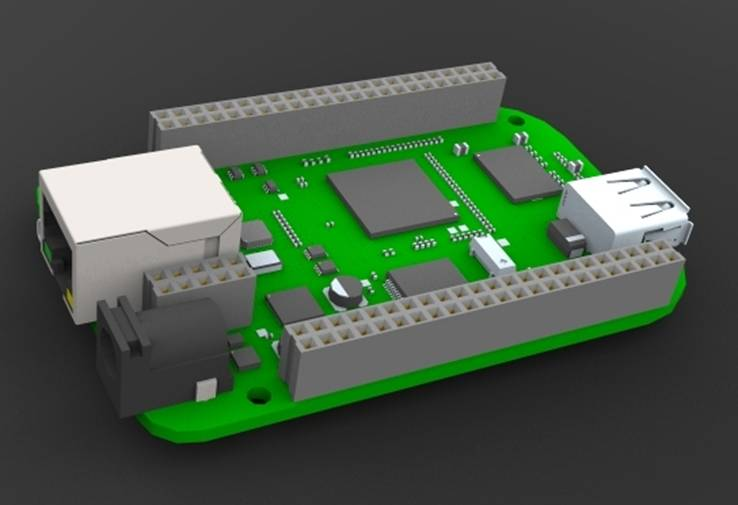
\includegraphics[width=0.6\linewidth]{beaglebone.jpg}
      \caption{Příklad plošného spoje s mnoha druhy integrovaných obvodů, vyžadující odlišné 
               napájecí úrovně}
      \label{SPICE:Basso_intro}
    \end{figure}

%---------------------------------------------------------------------------------------------------
%=============== Kapitola: Amplifiers =============================================================
  % !TeX spellcheck = cs_CZ
{\tikzset{external/prefix={tikz/AES/}}
 \tikzset{external/figure name/.add={ch02_}{}}
%---------------------------------------------------------------------------------------------------
% file amplifier.tex
%---------------------------------------------------------------------------------------------------
%============================ Kapitola: Zesilovače==================================================
\chapter{Zesilovače}
\minitoc

  V této kapitole se budeme zabývat rozbory vlastností základních obvodů a jejich účelným
  spojováním do funkčních bloků určených pro zesilování signálů. \cite[p.~101]{Neumann}
  
  \section{Zjednodušení výpočet tranzistorového ze\-si\-lo\-va\-če}
    Přesný výpočet tranzistorového zesilovače vychází z určení dvojbranových pa\-ra\-me\-trů
    tranzistoru a pokračuje sestavením matice obvodu a řešením této matice. Při použití vybraných
    rovnic matematických modelů pro programy SPICE lze dojít ke zjednodušenému řešení, ve kterém se
    některé parametry zanedbají a sestavené náhradní schema pak řešit libovolnou metodou. Přesto
    dostaneme výsledky s přesností, která pro obvyklé technické řešení postačuje.

    \subsection{Obecná převodní charakteristika bipolární tranzistoru}
      Převodní charakteristika udává závislost výstupního proudu na vstupním napětí. Pro zapojení
      \texttt{SE} představuje převodní charakteristiku exponenciální závislost kolektorového proudu
      na napětí mezi bází a emitorem. Strmost je dána derivací funkce (tečnou) v daném pracovním
      bodě a odpovídá parametru $\mathrm{y_{21}}$.

} % tikzset
%---------------------------------------------------------------------------------------------------
\printbibliography[title={Seznam literatury}, heading=subbibliography]
\addcontentsline{toc}{section}{Seznam literatury}

%=============== Kapitola: Signal generators ======================================================
  % !TeX spellcheck = cs_CZ
%---------------------------------------------------------------------------------------------------
% file oscillator.tex
%---------------------------------------------------------------------------------------------------
%======================== Kapitola: Generátory signálů==============================================
\setchaptertoc
\chapter{Generátory signálů}


  \textbf{Generátory signálů} jsou elektronické obvody, které za určitých podmínek generují 
  jednorázový nebo periodický signál. Na rozdíl od zesilovačů nejsou buzeny z vnějších zdrojů 
  signálů, patří tedy mezi \emph{autonomní obvody}.
  
  \begin{itemize}[noitemsep]
    \item \emph{Podle druhu vyráběných signálů:}
      \begin{itemize}
        \item neperiodických průběhů (jednorázových)
        \item periodických průběhů.
      \end{itemize}
    \item  \emph{Podle tvaru generovaného signálů:}
    \begin{itemize}
      \item harmonických signálů - \emph{oscilátory}
      \item impulzních průběhů - \emph{klopné obvody}
      \item funkční generátory - vytvářejí různé periodické průběhy jako trojúhelníkové, pilovité, 
            můžeme sem zařadit také generátory speciálních průběhů, jako jsou generátory, televizního signálů
            apod.
    \end{itemize} 
  \end{itemize}
  
  Mezi hlavní vlastnosti generátorů zahrnujeme tyto parametry:
  \begin{itemize}[noitemsep]
    \item kmitočet (perioda) kmitů
    \item stabilita kmitočtu a amplitudy
    \item doba náběžné a sestupné hrany impulzů - v \emph{klopných obvodech} 
    \item zkreslení harmonického průběhu - u \emph{oscilátorů}.
  \end{itemize}

  \section{Generátory harmonických signálů - oscilátory}
    Základními typy oscilátorů jsou:
    \begin{itemize}[noitemsep]
      \item Jednobranové LC oscilátory, též nazývané oscilátory se záporným diferenciálním odporem 
            (\emph{Negative Resistance Oscillators});
      \item Zpětnovazební oscilátory;
      \item Oscilátory RC;
      \item LC oscilátory;
      \item Krystalem řízené oscilátory.
    \end{itemize}

    Pro pásmo nízkých kmitočtů do několika set kHz může být sinusový signál generován oscilátorem s 
    RC selektivním zpětnovazebním obvodem, pro vyšší kmitočty jsou používány LC oscilátory. Pro 
    velmi přesné a stabilní oscilátory jsou využívány oscilátory řízené krystaly.
    
    \subsection{LC oscilátory se záporným diferenciálním odporem}
      Připojíme-li k paralelnímu rezonančnímu LC obvodu zdroj proudu o proměnném kmitočtu podle 
      obr. \ref{AES:fig_MUE6_311b}, na kterém jsou sériové ztrátové odpory přepočítány na paralelní 
      vodivost \(G_p\), můžeme získat modulové charakteristiky podle obr. \ref{AES:fig_MUE6_311a}. 
      Kmitočtová závislost přenosu je závislá na velikosti činitele jakosti obvodu \(Q\) (na 
      velikosti činných ztrát v obvodu). Čím užší je rezonanční křivka a stabilnější kmitočet 
      \(\omega_0\), tím přesnější a stabilnější je kmitočet oscilátoru.

      \begin{figure}[ht!]
        \centering     
        \subcaptionbox{\label{AES:fig_MUE6_311a}}{\luafigure[0.5]{MUE6_311a.pdf}} 
        \subcaptionbox{\label{AES:fig_MUE6_311b}}{\luafigure[0.4]{MUE6_311b.png}}  \\
        \subcaptionbox{\label{AES:fig_MUE6_311c}}{\luafigure[0.4]{MUE6_311c.png}} 
        \subcaptionbox{\label{AES:fig_MUE6_311d}}{\luafigure[0.5]{MUE6_311d.pdf}}  \\
        \subcaptionbox{\label{AES:fig_MUE6_311e}}{\luafigure[0.5]{MUE6_311e.pdf}} 
        \caption{a) Modulové charakteristiky paralelního rezonančního obvodu pro napěťový přenos.
                 b) model paralelního rezonančního obvodu a jeho napájení ze zdroje o proměnném 
                 kmitočtu, c) přeměna rezonančního obvodu v oscilátor, d) časová závislost napětí 
                 na svorkách ztrátového LC obvodu po rozkmitání, d) výstupní napětí bezeztrátového 
                 LC obvodu 
                 \cite[s.~135]{Dolecek2009}.}
        \label{AES:fig_MUE6_311}
      \end{figure}
      
      Na obr. \ref{AES:fig_MUE6_311c} je nakreslen paralelní rezonanční obvod, u kterého do obvodu 
      po přepnutí spínače z polohy \(1\) do polohy \(2\) připojujeme předem nabitý kondenzátor. V 
      obvodu vzniknou vlastní tlumené kmity o kmitočtu \(\omega_0\). Obvod lze popsat diferenciální 
      rovnicí
      \begin{equation}\label{AES:eq_osc04}
        \dder{i}{t} + \frac{R}{L}\cdot\der{i}{t} + \omega^2 i = 0
      \end{equation}
      Rovnice má řešení
      \begin{equation}
        i(t) = I_{0}e^{-\delta t}\sin\omega_v t  \qquad u(t) = U_{0}e^{-\delta t}\cos\omega_v t
      \end{equation}
      kde \(I_0\) je \emph{počáteční amplituda proudu}, \(U_0\) je \emph{počáteční amplituda napětí 
      na kapacitoru}, \(\delta = \frac{R}{2L}\) je \textbf{činitel tlumeni obvodu}, \(\omega_0 
      =\frac{1}{\sqrt{LC}}\) je \textbf{rezonanční kmitočet} a \(\omega_v = \sqrt{\omega^2_0 - 
      \delta^2}\) je \textbf{vlastní kmitočet volných kmitů} obvodu. 
      
      Ze vztahu (\ref{AES:eq_osc04}) je zřejmé, Že je-li činitel tlumeni a \textbf{kladný} je 
      kmitání \textbf{tlumené}, je-li a \textbf{záporný} je kmitání \textbf{netlumené}, je-li 
      \(\delta = 0\) mají kmity konstantní amplitudu. Velikost činitele tlumení je závislá na 
      velikosti rezistoru \(R\), který modeluje ztráty v rezonančním obvodu viz obr. 
      \ref{AES:fig_MUE6_311d}, \ref{AES:fig_MUE6_311e}.
      
      V reálném obvodu je vždy \(\delta > 0\) a proto pozorujeme tlumené kmity, jejichž amplituda 
      klesá exponenciálně podle vztahu 
      \begin{equation}\label{AES:eq_osc02}
        u(t) = U_{ss}e^{-\delta t},
      \end{equation}
      kde \(u(t)\) představuje časovou závislost amplitudy kmitů na svorkách paralelního LC obvodu. 
      Dosáhnout nulového tlumení je možné sériovým zapojením rezistoru \(-R_N = R\) - tedy 
      rezistoru se \textbf{záporným odporem}. K tomu by bylo zapotřebí najít takovou součástku, 
      jejíž voltampérová charakteristika vykazuje úsek se zápornou derivací. Hledáme tedy součástky 
      které mají voltampérovou charakteristiku jako je na obr. \ref{AES:fig_AES62a} nebo 
      \ref{AES:fig_AES62b}.
      
      \begin{figure}[ht!]
        \centering  
        \subcaptionbox{nelinearita typu \textbf{S} \label{AES:fig_AES62a}}{\luafigure[0.5]{AES_62a.pdf}}
        \subcaptionbox{nelinearita typu \textbf{N} \label{AES:fig_AES62b}}{\luafigure[0.5]{AES_62b.pdf}}                                          
        \caption{Voltampérové charakteristiky s úseky vykazující záporný diferenciální odpor 
        \cite[s.~93]{Koucky1997}}
        \label{MIT:fig_AES_62}
      \end{figure}
      
      Pro sériový model kmitavého obvodu obr. \ref{AES:fig_AES63a} je použitelná nelinearita 
      \texttt{typu S} (např. lavinová dioda), pro paralelní model kmitavého obvodu obr. 
      \ref{AES:fig_AES63b} je použitelná nelinearita \texttt{typu N} (např. tunelová dioda) 
      \cite[s.~93]{Koucky1997}.

      \begin{figure}[ht!]
        \centering  
        \subcaptionbox{sériový rezonanční obvod   \label{AES:fig_AES63a}}{\luafigure[0.5]{AES_63a.pdf}} 
        \subcaptionbox{paralelní rezonanční obvod \label{AES:fig_AES63b}}{\luafigure[0.5]{AES_63b.pdf}}                                           
        \caption{ }
        \label{MIT:fig_AES_63}
      \end{figure}
      
      Na velikosti ztrátového odporu \(R\) závisí velikost činitele tlumení \emph{(damping factor)} 
      obvodu podle vztahu:
      \begin{equation}\label{AES:eq_osc01}
        \delta = \frac{R}{2L} \qquad [rad/s]
      \end{equation}
      
      LC oscilátory obsahují klasický rezonanční obvod, jehož rezonanční kmitočet je určen 
      \textbf{Thomsonovým vztahem}:
      \begin{equation}\label{AES:eq_osc03}
        f_0 = \frac{1}{2\pi\cdot\sqrt{LC}} \quad [Hz], \;\text{nebo}\; 
        \omega_0 = \frac{1}{\sqrt{LC}} \quad [rad/s].
      \end{equation}
      
%---------------------------------------------------------------------------------------------------
%=============== Kapitola: Operační zesilovače ====================================================
  % !TeX spellcheck = cs_CZ
%---------------------------------------------------------------------------------------------------
% file opamp.tex
%---------------------------------------------------------------------------------------------------
%================================ Kapitola: Zesilovače==============================================
\setchaptertoc
\chapter{Operační zesilovače}\label{aesIchIII}

  \section{Základní pojmy}\label{aesIchIIIsecI}
    \subsection{Operační zesilovač}\label{aesIchIIIsecIssecI}
      \emph{Operační zesilovače} (\texttt{OZ}, aj: \texttt{opamp}) původně vznikly jako složité
      elektronické obvody pro náročné použití při zpracování analogových (spojitě se měnících)
      stejnosměrných a nízkofrekvenčních střídavých signálů v analogových počítačích, ve kterých
      realizovaly matematické operace. Aby se konstrukce analogových počítačů co nejvíce
      zjednodušila, bylo třeba unifikovat jejich jednotlivé části. Nejdůležitějším prvkem byl právě
      operační (dříve také nazývaný počítací) zesilovač. Protože měl vyhovět nejrůznějším
      požadavkům, bylo nutné, aby měl některé speciální vlastnosti \cite[s.~12]{Belza2004}. 

      \begin{figure}[ht!]  %\ref{aes:fig044}
        \centering
        \luafigure[0.4]{aes_fig044.jpg}
        \caption{První komerčně dostupný operační zesilovač \texttt{K2-W} z roku 1953
                \cite[s.~H.20]{Jung2005}}
        \label{aes:fig044}
      \end{figure} 

      Historie vývoje operačních zesilovačů je spjata s vývojem elektronek již od doby druhé světové
      války a je velice dobře popsána v příručce od \texttt{Analog Devices} \cite{Jung2005}. Vývoj
      je zde dokumentován také citací patentů. Tato éra vrcholí v roce 1953, kdy G. A. Philbrick
      uvedl na trh první komerčně dostupný operační zesilovač \texttt{K2-W} (obr. \ref{aes:fig044}).
      Elektronky byly později nahrazeny tranzistory a polovodičovými diodami. 
      
      Moderní polovodičová technologie umožnila vznik \texttt{OZ} v podobě levného integrovaného
      obvodu s malým počtem vývodů, který má nepatrnou spotřebu, je odolný proti přetížení a
      umožňuje jednoduše realizovat nejrůznější elektronická zařízení.
    
      V dnešním pojetí je možné vymezit operační zesilovač jako stejnosměrný zesilovač s velkým
      zesílením a malým vlastním rušením, schopný stabilní činnosti v uzavřené zpětnovazební smyčce.
      Přesným význam bude vyložen v následujících kapitolách. Zde jen poznamenejme, že přívlastkem
      \emph{stejnosměrný} není myšleno horní omezení dynamických vlastností operačního zeslovače,
      nybrž naopak rozšíření spektra zpracovávaných signálů k nulové frekvenci, k nekonečně dlouhým
      periodám.\cite[s.~5]{Dostal}.

      \begin{figure}[ht!]  %\ref{aes:fig041}
        \centering
          \subcaptionbox{\label{aes:fig041a}}{\luafigure[0.33]{aes_fig041a.pdf}}                                                  
          \subcaptionbox{\label{aes:fig041b}}{\luafigure[0.33]{aes_fig041b.pdf}}                    
          \subcaptionbox{\label{aes:fig041c}}{\luafigure[0.33]{aes_fig041c.pdf}}
        \caption{Symbolická značka OZ s vyznačenými signálovými svorkami (a) 
                a skutečná realizace zemní svorky (b, c) (\cite[s.~5]{Dostal})}
        \label{aes:fig041}
      \end{figure}

      Směr signálového toku operačním zesilovačem (dále jen OZ) od vstupu k výstupu je vyznačen
      trojúhelníkovým tvarem jeho symbolické značky na obr. \ref{aes:fig041a}. Tři ze čtyř
      znázorněných svorek představují tři signálové vývody skutečného operačního zesilovače a
      nazývají se \emph{invertující vstup, neinvertující vstup} a \emph{výstup}. Čtvrtá signálová
      svorka - zem - může být skutečná (obr. \ref{aes:fig041b}) nebo jen pomyslná (společná zem
      napájecích zdrojů na obr. \ref{aes:fig041c}), avšak v každém případě představuje symbolicky
      skupinu alespoň dvou napájecích vývodů určených pro přívod energie.  

      \begin{figure}[ht!]  %\ref{aes:fig042}
        \centering
        \subcaptionbox{\label{aes:fig042a}}{\luafigure[0.45]{aes_fig042a.jpg}}                                                 
        \subcaptionbox{\label{aes:fig042b}}{\luafigure[0.45]{aes_fig042b.jpg}}                    
        \caption{Přiřazení a orientace vstupních a výstupních napětí a proudů (a). Ve zjednodušeném 
                způsobu kreslení se zemní svorka vynechává (b). (\cite[s.~6]{Dostal})}
        \label{aes:fig042}
      \end{figure}

      Vedle signálových a napájecích vývodů má operační zesilovač podle potřeby ještě další vývody,
      určené např. pro úpravu dynamických charakteristik, pro nulování ofsetu, pro nastavení
      klidového odběru apod.

      Zemní signálová svorka tvoří referenční bod pro zbývající tři signálové svorky. Přiřazení
      kladných smyslů vstupních napětí \(u^-\), \(u^+\), výstupního napětí \(u_o\), vstupních proudů
      \(i^-\), \(i^+\) a výstupního proudu \(i_0\), ukazuje obr. \ref{aes:fig042a}. Nehrozí-li
      nedorozumění, může se zem ze značky zesilovače vypustit. Svorková napětí, vztažená i nadále k
      zemi, se pak vyznačí jen připsáním symbolu (obr. \ref{aes:fig042b}).

      Absolutní velikosti signálových napětí \(u^-\), \(u^+\) a \(u_o\) jsou omezeny napětím
      napájecích zdrojů. U zesilovačů s dvojitým napájením se používají dvě zpravidla vzájemně
      opačná napájecí napětí \(U_s^+\) a \(U_s^-\) (obr. \ref{aes:fig041c}), rovná např.
      +\SI{+15}{\volt} a \SI{-15}{\volt}. Odpovídající rozkmit obou vstupních napětí a výstupního
      napětí je pak rovněž souměrný do obou polarit, např. v mezích \(\pm\)\SI{10}{\volt}. U
      zesilovačů s jednoduchým napájením se používá jedno napájecí napětí \(U_s\) (obr.
      \ref{aes:fig041b}), rovné např. \SI{5}{\volt}. Odpovídající rozkmit obou vstupních napětí a
      výstupního napětí je pak pouze do jedné polarity, např. v mezích \num{0}/+\SI{4}{\volt}.

      Výstupní proud \(i_0\), se přizpůsobuje zátěži. Ta může být pasivní i aktivní, s přípustnými
      pracovními body (\(u_o\), \(i_0\) ve všech čtyřech kvadrantech, v případě dvojitého napájení.

      Charakteristickou přenosovou vlastností operačního zesilovače je jeho velká citlivost k
      rozdílu obou vstupních napětí a necitlivost k jejich absolutní velikosti. Tato vlastnost
      přivádí k pojmům \textbf{souhlasného vstupního napětí} \(u_{cm}\) jako superponované společné
      složky obou vstupních napětí, kterou zesilovač potlačuje, a \textbf{diferenčního vstupního
      napětí} \(u_D\), na které zesilovač reaguje. Zatímco přiřazení diferenčního vstupního napětí
      je nasnadě (obr. \ref{aes:fig042a}),
      \begin{equation}\label{aes:eq026}
        u_D = u^- - u^+,
      \end{equation}
      jsou možnosti definice souhlasného vstupního  napětí neomezené, 
      \begin{equation}\label{aes:eq027}
        u_{CM} = u^+ + Ku_D,
      \end{equation}
      dané volitelností konstanty \(K\). Dvě prakticky používané volby jsou \(K=\frac{1}{2}\) a
      \(K=0\). První volba zachovává symetrii, 
      \begin{equation*}
        u_{CM} = \dfrac{u^- + u^+}{2},
      \end{equation*}
      ale vede k formálním obtížím při definici parametrů operačního zesilovače. Proto se dává
      přednost druhé volbě, při které je souhlasné vstupní napětí ztotožněno s napětím
      neinvertujícího vstupu: 
      \begin{equation*}
        u_{CM} = u^+,
      \end{equation*}
      Tato druhá volba je opodstatněná také funkcí uzavřené zpětnovazební smyčky v nejčastějších
      případech, ve kterých zastává neinvertující vstup úlohu vnucené reference, s níž se
      invertující vstup samočinně srovnává. Rozdíl mezi oběma definicemi je nadto prakticky
      nepodstatný vzhledem k nepatrné velikosti diferenčního vstupního napětí ve srovnání s rozsahem
      souhlasného vstupního napětí. 

      %--Zesílení Ideálního Operačního Zesiovače----------------------
      % !TeX spellcheck = cs_CZ
\begin{mdframed}[style=mdexam]
  \begin{example}\label{aes:exam004}
    Běžné OZ mají zesílení \(A = \numrange{20000}{2000000}\). Znamená to, že pro výstupní napětí
    \SI{10}{\V} je mezi kladným a záporným vstupem napětí \(u_D
    =\frac{\SI{10}{\V}}{\numrange{2000000}{20000}}\) = \SIrange{5}{500}{\uV}. V praxi to většinou
    znamená, že rozdílové napětí \(u_D\) považujeme za nulové pro jakékoliv výstupní napětí \(u_0\).
    Jak se později ukáže, tato úvaha je velmi důležitá. Podmínku \(u_D = 0\) se snažíme zajistit za
    všech okolností. Vede to k požadavku, aby zesílení ideálního OZ bylo nekonečně velké (u reálného
    co největší) (\cite[s.~14]{Puncochar1996}).    
  \end{example}
\end{mdframed}
      %---------------------------------------------------------------
    
    \subsection{Operační obvod}\label{aesIchIIIsecIssecII} 
      Samotný operační zesilovač je jen částí výsledného zařízení, i když zpravidla částí
      nejdůležitější. Nedílnou druhou, funkčně určující část tvoří vnější zpětnovazební síť. Obecné
      uspořádání s jedním operačním zesilovačem, signálovým zdrojem a zátěži ukazuje obr.
      \ref{aes:fig045}. Zpětnovazební síť, znázorněná vyšrafovaným obrazcem a sestavená z pasivních
      i aktivních elektronických a elektromechanických součástek, je ukončena vytknutými styčnými
      uzly, jejichž prostřednictvím je spojena se signálovými svorkami operačního zesilovače,
      signálového zdroje a zátěže. Celek operačního zesilovače, zpětnovazební sítě, signálového
      zdroje a zátěže tvoří operační obvod. Jeho vstupní veličinou je vstupní napětí \(u_s\) nebo
      vstupní proud \(i_s\) na svorkách signálového zdroje, jeho výstupní veličinou je výstupní
      napětí \(u_o\) nebo výstupní proud \(i_0\) na svorkách zátěže. Za povšimnutí stojí, že výstup
      operačního obvodu nemusí být obecně totožný s výstupem operačního zesilovače a zem zesilovače
      (zem napájecích zdrojů podle obr. \ref{aes:fig041b}, \ref{aes:fig041c} nemusí být přímo
      spojena s jednou svorkou signálového zdroje nebo zátěže, i když tomu tak zpravidla je.
      \begin{figure}[ht!] % \ref{aes:fig045}
        \centering
        \luafigure[1]{aes_fig045.png}
        \caption{Operační obvod s jedním operačním zesilovačem, jedním signálovým zdrojem a jednou 
                 zátěži. (\cite[s.~8]{Dostal})}
        \label{aes:fig045}
      \end{figure}

      S výjimkou operačních obvodů, které fungují jako referenční zdroj, oscilátor nebo
      multivibrátor, je výstupní veličina (\(u_0\), \(i_0\)) v jistém vztahu k vstupní veličině
      (\(u_s\), \(i_s\)). Tento vztah vyjádřený matematicky se nazývá operační rovnice obvodu.

      Nejcennější vlastností obvodů s operačními zesilovači je značná necitlivost operační rovnice
      jak k rozptylu parametrů samotného operačního zesilovače, tak ke změnám zátěže a často i
      signálového zdroje (ke změnám jejich zatěžovacího nebo vnitřního odporu). První skutečnost
      vede k definici ideálního operačního zesilovače (odst. \ref{aesIchIIIsecIssecIII}), druhá
      skutečnost vede ke zúženému chápání operačního obvodu jako pouhého spojení operačního
      zesilovače a zpětnovazební sítě. Necitlivost operační rovnice k vlastnostem přirozeně
      nestálého aktivního prvku - zesilovače - vtiskuje návrhu operačních obvodů rys matematické
      předvídatelnosti chování. Operační rovnice se tak stává spíše charakteristikou samotné
      zpětnovazební sítě.

      Operační obvod podle obr. \ref{aes:fig045} může být rozšířen připojením dalších signálových
      zdrojů, operačních zesilovačů a zátěží. Realizace zpětnovazební sítě nemusí být omezena jen na
      elektrické prostředky. Signálová smyčka se může uzavírat i přes jiné druhy signálu než
      elektrické napětí nebo elektrický proud: Přes magnetickou indukci, Lorentzovu sílu, mechanické
      napětí, deformaci a piezoelektrický náboj, přes teplo, teplotu a termoelektrické napětí, přes
      světlo a fotoemisní proud, přes polohu servomotoru a napětí polohového potenciometru apod.
      Jedinou, avšak zásadní svazující podmínkou je \emph{zachování} zpětnovazební stability
      výsledné uzavřené smyčky.


    \subsection{Ideální OZ a operační obvod}\label{aesIchIIIsecIssecIII}
      Paradoxním cílem, ke kterému směřuje snažení každého konstruktéra operačních zesilovačů, je
      vytvoření zesilovače v aplikaci neviditelného v tom smyslu, že neovlivňuje znění příslušné
      operační rovnice. Jeho abstrakcí je ideální operační zesilovač, užitečná představa, která
      umožňuje rychlou analýzu jmenovitého (zamýšleného) chování operačního obvodu nebo umožňuje
      syntézu operačního obvodu podle zadaného matematického nebo jen funkčního popisu, s výsledky
      použitelnými bezprostředně a přesně ve skutečné aplikaci. Skutečné operační zesilovače se
      svému ideálu v různé míře přibližují, přičemž těsnější přiblížení je při daném stavu
      technologie zpravidla zaplaceno větší obvodovou složitosti a vyšší cenou.
      \begin{itemize}[noitemsep]
        \item Ideální operační zesilovač je operační zesilovač s nulovým diferenčním vstupním
              napětím a s nulovými vstupními proudy pro jakékoliv výstupní vybuzení a jakékoliv
              souhlasné vstupní vybuzení: 
              \begin{equation}\label{aes:eq029}
                u_D, i^-, i^+ = 0 \quad\text{pro libovolné}\quad u_0, i_0, u_{CM}.
              \end{equation}
        \item ideální operační obvod je operační obvod vzniklý myšlenou náhradou skutečného
              operačního zesilovače ideálním operačním zesilovačem.     
        \item ideální operační rovnice je operační rovnice ideálního operačního obvodu.
      \end{itemize}

      Význam těchto abstrakcí oceníme v kapitole \ref{aesIchIVsecI}. Jak je vidět z rov.
      (\ref{aes:eq029}), je dokonalost operačního zesilovače určena dokonalosti jeho vstupní strany
      (odchylkou jeho diferenčního vstupního napětí a vstupních proudů od nuly).

      Řečeno jazykem kapitoly \ref{aesIchIIIsecII} má ideální operační zesilovač na všech
      frekvencích nekonečné zesilení, nekonečné potlačení souhlasného vstupního napětí, nekonečné
      souhlasné vstupní impedance a nulové vstupní rušivé zdroje, jak je rovněž možné vysledovat z
      rov. (\ref{aes:eq029}). Velikost diferenční vstupní impedance a výstupní impedance je vzhledem
      k nekonečnému zesílení nepodstatná. Protože však skutečné hodnoty těchto impedanci u
      skutečného zesilovače (s konečným zesílením) zhoršují dynamické chyby operačního obvodu,
      spojuje se s představou ideálního operačního zesilovače také nekonečná diferenční vstupní
      impedance a nulová výstupní impedance. Katalogový list ideálního operačního zesilovače tedy
      obsahuje samé nuly a nekonečna.

      Početní analýza operačního obvodu v určitém směru (např. výpočet šumu, zesílení) se velmi
      zjednoduší, jestliže se hned zpočátku zanedbají nepodstatné okolnosti, tj. jestliže se
      nepodstatné parametry operačního zesilovače idealizují. Idealizovaný operační zesilovač je
      operační zesilovač, jehož některé parametry mají ideální (nulovou nebo nekonečnou) velikost.

    \subsection{Shrnutí}\label{aesIchIIIsecIssecIV}
      \begin{enumerate}[noitemsep]
        \item Operační zesilovač má čtyři signálové svorky, i když se často kreslí jen tři - oba 
              vstupy a výstup. Čtvrtou signálovou svorkou je zem.
        \item Souhlasné napětí $u_{CM}$ je totožné s napětím jeho neinvertujícího vstupu $u^+$.
        \item Ideální operační zesilovač má za všech okolností nulové diferenční vstupní napětí a  
              nulové vstupní proudy.
      \end{enumerate}
    
  \section{Parametry OZ}\label{aesIchIIIsecII}
    Ideální operační zesilovač je nedosažitelná abstrakce. K posouzení kvality sku\-teč\-ného 
    operačního zesilovače slouží řada funkčních parametrů jako soubor dat, která lze zjistit 
    měřením na svorkách.
   
    Operační zesilovač, jako každý aktivní elektronický obvod, je obvod nelineární. Protože však
    prostředky analýzy nelineárních obvodů jsou omezené a pracné, je namístě otázka po přijatelné
    linearizaci. Její oprávněnost je podpořena tím, že parametry operačního zesilovače nevystupují v
    operační rovnici jako veličiny určující, nýbrž jako příčiny chyb, a že tedy jejich případná
    lineární aproximace zanáší jen nepřesnost druhého řádu, chybu v chybě.

    Odpověď na položenou otázku je příznivá. Všechny funkční charakteristiky operačního zesilovače
    připouštějí linearizaci bez přílišného odklonu od skutečnosti. Odpovídající kvazilineární
    parametry jsou podkladem lineárního modelu operačního zesilovače. Ostatní parametry jsou
    podstatné nelinearity, které tvoří meze jeho lineární oblasti.
    
    \subsection{Lineární model a parametry}\label{aesIchIIIsecIIssecI}
      Obr. \ref{aes:fig046} ukazuje úplný \emph{lineární model} operačního zesilovače. Se zřetelem k
      pozdější analýze chyb operačního obvodu je vhodné rozdělit znázorněné lineární parametry na
      \textbf{aditivní} a \textbf{multiplikativní}.
      \begin{itemize}[noitemsep]
        \item \textbf{Aditivní parametry} zahrnují náhradní rušivé zdroje náhodných fluktuací:
              \(E_R\), \(I_R^-\), \(I_R^+\), které způsobují aditivní chyby operačního obvodu
              nezávislé na jeho signálovém vybuzení.
        \item \textbf{Multiplikativní parametry} představované čtyřmi odpory \(R_D\), \(R^-_{CM}\),
              \(R^+_{CM}\), \(R_0\) a dvěma řídicími konstantami \(-A\), \(1/X\) závislých
              generátorů, vystihují pasivní a přenosové vlastnosti OZ a způsobují multiplikativní
              chyby operačních obvodu úměrné jeho signálovému vybuzení.
      \end{itemize}
      Vnitřní, na svorkách neměřitelný napěťový úbytek \(e_D\) na odporu \(R_D\) zastává v tomto
      modelu vazbu mezi vstupem a výstupem.
     
      Při práci s proměnnými signály v časové nebo ve frekvenční oblasti se význam použitých symbolů 
      vhodně rozšíří na impedance, operátorové přenosy apod.

      \begin{figure}[ht!] % \ref{aes:fig046}
        \centering
        \luafigure[1]{aes_fig046.pdf}
        \caption{Lineární model operačního zesilovače. (\cite[s.~14]{Dostal}}
        \label{aes:fig046}
      \end{figure}

      S obvodovým modelem na obr. \ref{aes:fig046} je rovnocenný \emph{matematický model},
      představovaný soustavou tří rovnic
      \begin{subequations}\label{aes:eq030}
        \begin{align}
          u_D &= E_R   + \dfrac{u_{CM}}{X} - \dfrac{u_0 + R_0i_0}{A},     \label{aes:eq030a}   \\
          i^- &= I_R^- + \dfrac{u_{CM}}{R_{CM}^-}
                       - \dfrac{u_0 + R_0i_0}{A(R_D\parallel R_{CM}^-)},  \label{aes:eq030b}   \\ 
          i^+ &= I_R^+ + \dfrac{u_{CM}}{R_{CM}^+}
                       + \dfrac{u_0 + R_0i_0}{AR_D}.                      \label{aes:eq030c}
        \end{align}
      \end{subequations}
      \(R_D\parallel R_{CM}^-\) značí paralelní kombinaci odporů \(R_D\) a \(R_{CM}^-\)
      
      Ekvivalence obou modelu je podložena Kirchhoffovými zákony psanými pro vstupní svorky
      operačního zesilovače při uvážení rovnosti \(e_D = -\frac{u_0 +R_0i_0}{A}\). Na vysvětlení to
      ukážeme pro vstupní proud \(i^-\). Proud tekoucí do invertujícího vstupu ma podle obr.
      \ref{aes:fig046} velikost
      \begin{equation*}
        i^- = I_R^- + \dfrac{u_{CM} + e_D}{R_{CM}^-} + \dfrac{e_D}{R_D} 
            = I_R^- + \dfrac{u_{CM}}{R_{CM}^-} + \dfrac{e_D}{(R_D\parallel R_{CM}^-)},
      \end{equation*}
      což souhlasí s rov. \ref{aes:eq030b}.

      Definice, které následují, předvádějí jednotlivé parametry lineárního modelu v termínech
      svorkových napětí a proudů a jejich změn. Každý parametr je znázorněn svým základním měřícím
      obvodem, který používá konceptu pomocného ideálního operačního zesilovače k imitování podmínek
      definice.

      Znění některých definici se poněkud liší od formulaci používaných výrobci operačních
      zesilovačů v katalogových listech. Katalogové údaje často představují spíše záruky řádného
      chování, které přísluší kombinovanému vlivu několika dílčích parametrů (např. zesílení při
      jmenovité zátěži), nebo vycházejí ze zavedených měřicích schémat, zatímco posláním této
      kapitoly je vytvoření jednodchého nástroje pro lineární a nelineární analýzu operačního obvodu
      v následující části \ref{aesIchIV}. Zmíněné odchylky jsou prakticky nepodstatné.
    
      \subsubsection{Vstupní rušivé zdroje}\label{aesIchIIIsecIIssecII}
        Reálné vlastnosti OZ se nejvíce projevují superponovanou výstupní chybovou složkou,
        způsobenou šumovými vlastnostmi součástek zesilovačef, jejich stárnutí a jejich citlivost na
        vnější vlivy. Největší podíl tohoto šumu v šírším smyslu slova přísluší vstupním obvodům.
        Pro kvantitativní posouzení je proto přirozená volba ekvivaletních vstupních rušivých
        zdrojů, virtuálně rovnocenných svým účinkém šumovému projevu skutečného OZ. Z praktických
        měřicích se ujala definice založená nikoliv na Ekvivalenci, nýbrž na kompenzaci skutečných a
        náhradních rušivých účinků.
        \begin{itemize}[noitemsep]
          \item \emph{Vstupní rušivé napětí} \(E_R\) je velikost diferenčního vstupního napětí při
                nulovém souhlasném vstupním napětí, která přísluší nulovému výstupnímu napětí
                naprázdno.
          \item \emph{Vstupní rušivý proud} \(I_R^-\), resp. \(I_R^+\) je velikost proudu
                invertujícího resp. neinvertujícího vstupu při nulovém souhlasném vstupním napětí,
                která přísluší nulovému výstupnímu napětí naprázdno.
        \end{itemize}

        Pro objasnění podmínek definice ukážeme, že takto definované vstupní rušivé zdroje jsou
        skutečně totožné s parametry \(E_R\), \(I_R^-\), \(I_R^+\) lineárního modelu na obr.
        \ref{aes:fig046}. 

        Ve stavu naprázdno je napěťový úbytek na odporu \(R_0\) nulový. Podmínka nulového výstupního
        napětí naprázdno (\(u_0=0\), \(i_0=0\), \(e_0=0\)) vede k nulovému vnitřnímu napětí \(e_D =
        - \frac{e_0}{A}\) a k nulovému vnitřnímu proudu \(\frac{e_D}{R_D}\) mezi oběma vstupy.
        Uzemněním neinvertujícího vstupu (\(u_{CM} = 0\)) se anuluje vnitřní závislé vstupní napětí
        \(e_{CM} = \frac{u_{CM}}{X}\) a anulují se také vnitřní proudy \(\frac{u_{CM}}{R_{CM}^+}\) a
        \(\frac{u_{CM} + e_D}{R_{CM}^-}\) tekoucí přes odpory \(R_{CM}^+\) a \(R_{CM}^-\).
        Odpovídající velikosti diferenčního vstupního napětí a vstupních proudů jsou tedy
        \begin{equation}\label{aes:eq031}
          u_D = E_R, \quad i^- = I_R^-, \quad i^+ = I_R^+,
        \end{equation}
        jak stanoví definice. Vztahy \ref{aes:eq031} plynou samozřejmě také z rov. \ref{aes:eq030}
        pro \(u_{CM}\), \(u_0\) a \(i_0 = 0\).

        \luagraphic[0.8]{aes_fig047.pdf}{Základní měřicí obvod pro měření vstupních rušivých zdrojů. 
        (\cite[s.~16]{Dostal})}{aes:fig047}

        Definice vstupních rušivých zdrojů korespondují se základním měřicím obvodem na obr.
        \ref{aes:fig047}. Výstup měřeného OZ s uzemněným neinvertujícím vstupem je snímám pomocným
        ideálním OZ, který zastává úlohu nezatěžujícího nulového indikátoru. Výstup tohoto pomocného
        zesilovače samočinně nastavuje invertující vstup měřeného OZ tak, že jeho výstupní napětí
        naprázdno je nulové. Podle definice je okamžitá velikost takto nastaveného vstupního napětí
        \(u_D\) rovna okamžité velikosti vstupního rušivého napětí \(E_R\) a okamžité velikosti
        vstupních proudů \(I_R^+\) a \(I_R^-\).

      \subsubsection{Vstupní ofset a drift}\label{aesIchIIIsecIIssecIII}
        Všimněme si blíže spektrálního složení vstupních rušivých zdrojů, obr. \ref{aes:fig048}. Pro
        přesnost aplikací jsou obvykle rozhodující stejnosměrné a velmi zvolna proměnné složky,
        souhrnně označované jako \textbf{vstupní ofset} operačního zesilovače. Pásmo frekvencí
        těchto kvazistejnosměrných složek se vymezuje rozsahem \num{0} až \SI{0.01}{\Hz}. Vstupní
        ofset zahrnuje vstupní zbytkové napětí \(E_{OS}\) (stejnosměrnou složku vstupního rušivého
        napětí \(E_R\) a vstupní klidové proudy \(I_B^+\), \(I_B^-\) (stejnosměrné složky vstupních
        rušivých proudů \(I_R^+\), \(I_R^-\)).
              
        Oba vstupní klidové proudy se obyčejně liší málo. K vyjádření jejich všeobecné shody se
        zavádějí odvozené pojmy, \textbf{(průměrný) vstupní klidový proud} \(I_B\) jako jejich
        průměr\footnote{Zaručený katalogový údaj vstupního klidového proudu \(I_B\) se vztahuje na
        každý proud \(I_B^-\) a \(I_B^+\) zvlášť, nikoliv na jejich průměr.} a \textbf{vstupní
        zbytkový proud} \(I_{OS}\) jako jejich rozdíl:
        \begin{equation}\label{aes:eq090}
          I_B = \dfrac{I_B^- + I_B^+}{2}, \quad I_{OS} = I_B^- - I_B^+.
        \end{equation}
        
        \begin{figure}[ht!] % \ref{aes:fig048}  aes_fig048.tex/jpg
          \centering
          \luafigure[1]{aes_fig048.pdf}
          \caption{Terminologie a symboly vstupních rušivých zdrojů. (\cite[s.~16]{Dostal})}
          \label{aes:fig048}
        \end{figure}

        Chybu způsobenou vstupním ofsetem operačního zesilovače je možné vynulovat vnějším zásahem
        do operačního zesilovače samotného nebo do zpětnovazební sítě. Pro přesnost aplikací je
        důležitější nestálost ofsetu, označovaná jako \textbf{vstupní drift}. Jak bude zřejmé z
        dalšího, rozumí se driftem nejčastěji poměr změny ofsetu ke změně příčinného vlivu. S
        výjimkou samovolných časových změn (stárnutí) jde o vratné změny ofsetu v závislosti na
        kolísání pracovního prostředí zesilovače - teploty okolí a napájecího napětí. Se zřetelem k
        této nestabilitě se označuje ofset příslušející \emph{standardním podmínkám} (teplota
        +\SI{25}{\degreeCelsius}, napájecí napětí např. +\SI{15}{\V}) jako počáteční ofset.
        
        \begin{figure}[ht!] % \ref{aes:fig049}
          \centering
          \luafigure[1]{aes_fig049.jpg}
          \caption{Teplotní závislost vstupního zbytkového napětí \(E_{OS}(T)\). Všechny tři
                  znázorněné průběhy přísluší vyhovujícím zesilovačům podle tříbodové definice
                  (2.4b), a přesto může diferenciální drift \(\der{E_{OS}}{T}\) překročit zaručenou
                  mez \(\pm(\Delta E_{OS}/\Delta T)_M\). (\cite[s.~17]{Dostal})}
          \label{aes:fig049}
        \end{figure}

        Typický průběh vstupního zbytkového napětí s teplotou ukazuje graf a na obr. 2.4. Pro
        jednoznačnost katalogových údajů a pro jednoduchost měření se k charakterizaci nelineární
        závislosti \(E_{OS}(T)\) zavádí \textbf{průměrný teplotní drift} vstupního zbytkového napětí
        \(\Delta E_{OS}/\Delta T\) v daném intervalu teplot \(\Delta T\) jako poměr změny vstupního
        zbytkového napětí mezi krajními teplotami tohoto intervalu k jeho délce.   
        
        V nejjednodušším případě se obě krajní teploty ztotožní s dolní a horní hranicí \(T_L\) a
        \(T_H\) rozsahu pracovních teplot a stanoví se průměrný drift

        \begin{subequations}\label{aes:eq039}
          \begin{align}
            \left.\frac{\Delta E_{OS}}{\Delta T}\right\rvert_{LH} &= 
                                    \dfrac{E_{OS_H} - E_{OS_L}}{T_H - T_L}, \label{aes:eq039a} \\
            \left.\frac{\Delta E_{OS}}{\Delta T}\right\rvert_{L0} &= 
                                    \dfrac{E_{OS_0} - E_{OS_L}}{T_0 - T_L}, \label{aes:eq039b} \\
            \left.\frac{\Delta E_{OS}}{\Delta T}\right\rvert_{0H} &= 
                                    \dfrac{E_{OS_H} - E_{OS_0}}{T_H - T_0}, \label{aes:eq039c}
          \end{align}
        \end{subequations}

        Důkladnější postup, který lépe postihuje nelinearity typu \(U\) (graf b na obr.
        \ref{aes:fig049}), spočívá v rozdělení pracovního rozsahu při standardní teplotě \(T_0\) na
        dva intervaly (\(T_L\), \(T_0\)) a (\(T_0\), \(T_H\)) a ve stanovení dvou dílčích průměrných
        driftů.

        V každém uvedeném způsobu se změřený a vypočtený teplotní drift podle rov.
        (\ref{aes:eq039a}) nebo (\ref{aes:eq039b}) resp. (\ref{aes:eq039c}) porovná s katalogovým
        údajem zaručeného driftu \((\Delta E_{OS}/\Delta T)_M\). Vyšrafovaný motýlek s hranicemi
        \((+\Delta E_{OS}/\Delta T)_M\) a \(-(\Delta E_{OS}/\Delta T)_M\) vymezuje pole, do kterého
        musí padnout koncové body teplotních průběhů \(E_{OS}(T)\) vyhovujících zesilovačů a ve
        kterém obvykle leží celý průběh \(E_{OS}(T)\).

        Průměrný drift je ukazatel dostatečně výstižný pouze u závislostí blízkých k závislosti
        lineární, protože si všímá jen koncových bodů a nepřihlíží k chování uvnitř intervalu: dva
        zesilovače s velmi odlišnými průběhy \(a\) a \(c\) na obr. \ref{aes:fig049} mají v intervalu
        (\(T_0\), \(T_H\)) tentýž průměrný drift. Průměrný drift může být ukazatel i hrubě
        zkreslující, jak ukazuje graf c na obr. \ref{aes:fig049}, který přísluší zesilovači s
        nulovým průměrným driftem v intervalu (\(T_L\), \(T_0\)), a přesto zesilovači značně
        teplotně citlivému.

        Obdobným způsobem se zavádí i průměrný teplotní drift vstupního klidového a vstupního
        zbytkového proudu \(\Delta I_B/\Delta T\) a \(\Delta I_{OS}/\Delta T\). Nelinearita
        závislosti \(I_B(T)\) a \(I_{OS}(T)\) je výraznější a pojem průměrného driftu je spornější.
        Často se proto udávají jen zaručené maximální hodnoty obou proudu \(I_B\) a \(I_{OS}\) při
        standardní teplotě a při mezních pracovních teplotách.

        Dosud probírané teplotní změny se týkaly operačního zesilovače jako celku. Mnohem
        nebezpečnější mohou být poměrně malé \emph{teplotní diference} mezi jeho kritickými částmi,
        způsobené cizími tepelnými zdroji nebo vlastním ohřevem (po zapnutí napájení, po změnách
        zátěže, po zahlcení vstupu) a projevující se porušením vnitřní teplotní kompenzace
        diferenčních zesilovacích stupňů nebo vznikem termoelektrických napětí. Zvlášť citlivé jsou
        levné typy operačních zesilovačů následkem nevyvážené tepelné zpětné vazby uvnitř
        polovodičového čipu.

        \emph{Kolísání napájení} je druhou podstatnou příčinou změny ofsetu. Citlivost na změnu
        napájecího napětí \(U_S\) se udává \emph{průměrným napájecím driftem} vstupního zbytkového
        napětí \(\Delta E_{OS}/\Delta U_S\), vstupního klidového proudu \(\Delta I_B/\Delta U_S\) a
        vstupního zbytkového proudu \(\Delta I_{OS}/\Delta U_S\). V případě zbytkového napětí je
        tento drift bezrozměrný (udávaný v \si{\micro\volt\per\volt}) a analogicky k potlačení
        souhlasného napětí, bývá někdy uváděn v převráceném poměru jako \emph{potlačení napájecího
        napětí} \(\Delta U_S/\Delta E_{OS}\) a udáván v decibelech.

        U zesilovačů s dvojitým napájením se změnou \(\Delta U_S\) obvykle rozumí změna jednoho z
        napájecích napětí \(U_S^+\) nebo \(U_S^-\). Je ovšem možné si představit i současnou a
        stejnou změnu obou napájecích napětí, a to ve stejném nebo v opačném smyslu, obecně však
        není možné předem odhadnout, která z těchto možností je nepříznivější. Souhrnně lze říci, že
        v porovnání s jinými elektronickými výrobky a při uvážení dosahované přesnosti je operační
        zesilovač ke svému napájení velmi tolerantní. Výsledná nestabilita napájecího napětí 1 \% až
        10 \% je vyhovující, pokud napájecí zdroj neslouží zároveň jako referenční zdroj operačního
        obvodu.

        Samovolná časová \emph{změna} ofsetu jako projev stárnutí je nevratná, a proto
        neopakovatelná. Z toho důvodu nemůže být ani rozumně zaručována, a bud" je udána typickou
        hodnotou sejmutou na ověřovacím souboru zesilovačů, nebo není uváděna vůbec. Analogicky k
        oběma předchozím driftům se používá poměrový údaj průměrného časového driftu vstupního
        zbytkového napětí \(\Delta E_{OS}/\Delta t\), vstupního klidového proudu \(\Delta I_B/\Delta
        t\) a vstupního zbytkového proudu \(\Delta I_{OS}/\Delta t\), vztažený na interval dne,
        měsíce nebo roku. Při interpretaci je však nutné pamatovat, že časový drift není
        kumulativní, a že tedy údaj příslušející jednomu intervalu není možné lineárně přenášet na
        interval kratší ani delší.

      \subsubsection{Vstupní šum}\label{aesIchIIIsecIIssecIV}
        \emph{Vlastní šum} OZ je udán \textbf{vstupním šumovým napětím} \(E_N\) (šumovou složkou
        vstupního rušivého napětí \(E_R\)) a \textbf{vstupními šumovými proudy} \(I_N^-\) a \(I_N^+\)
        (šumovými složkami vstupních rušivých proudů \(I_R^-\) a \(I_R^+\) ). Vzhledem ke statistické
        povaze šumu se obvykle uvádí pouze společný údaj \(I_N\) s významem \(I_N^-\) nebo \(I_N^+\).
        Šumové napětí a šumové proudy jsou zpravidla nezávislé, ale někdy mohou obsahovat korelované
        složky (např. šumové napěťové úbytky na ochranných sériových vstupních rezistorech, korelované
        s průtokem vstupních šumových proudů).
        
        Šumové Zdroje \(E_N\) a \(I_N\) se charakterizují integrálně nebo spektrální hustotou.
        Integrální údaj, který přísluší šumovým složkám z určitého frekvenčního pásma, představuje buď
        \emph{efektivní} (rms), nebo \emph{mezivrcholovou} (pp) hodnotu\footnote{Z anglického
        root-mean-square (rms) a peak-to-peak (pp)} šumového napětí \(E_N\) a šumového proudu \(I_N\)
        v dostatečném časovém intervalu. Definice efektivní hodnoty šumu vychází běžným způsobem z
        ekvivalence tepelných účinků, avšak mezivrcholová hodnota vyžaduje bližšího vysvětlení.

        \begin{figure}[ht!] % \ref{aes:fig050}
          \centering
          \luafigure[1]{aes_fig050.jpg}
          \caption{Vztah mezivrcholové a efektivní hodnoty šumového napětí \(E_N\) při Gaussově
                  rozdělení výchylek. Tabulka uvádí pravděpodobnost výskytu velkých výchylek, které
                  přesahují specifikovanou mezivrcholovou hodnotu, udanou jako nasobek efektivní
                  hodnoty (střední kvadratické výchylky) \(\sigma\). (\cite[s.~20]{Dostal})}
          \label{aes:fig050}
        \end{figure}

        Většina šumů sleduje Gaussovo (normální) rozdělení okamžitých výchylek, Znázorněné
        pravděpodobnostní rozdělovací křivkou na obr. \ref{aes:fig050}. Plocha pod rozdělovací křivkou
        mezi dvěma amplitudami \(u_N\) je rovna pravděpodobnosti výskytu okamžité velikosti šumu
        \(u_N(t)\) mezi těmito amplitudami. Přestože je pravděpodobnost výskytu velkých výchylek malá,
        jsou jakkoliv velké výchylky přece možné. Aby změřený údaj nezávisel na subjektu pozorovatele
        (na jeho trpělivosti, tj. na době pozorování nebo na délce záznamu), Zavádí se mezivrcholová
        hodnota šumového průběhu statisticky: Časová pravděpodobnost výskytu větších výchylek, které
        přesahují udanou mezivrcholovou hodnotu, je rovna dohodnutému procentu. Jinak řečeno,
        mezivrcholová hodnota udává šířku šumového pásu, ve kterém leží převažující část šumového
        průběhu, přičemž časová pravděpodobnost přesažení udaného šumového pásu (udané mezivrcholové
        hodnoty) je rovna dohodnutému procentu.

        Tabulka v obr. \ref{aes:fig050} přiřazuje několik údajů mezivrcholové hodnoty Gaussova šumu,
        vyjádřených v násobcích efektivní hodnoty (střední kvadratické výchylky) \(\sigma\). K rychlé
        orientaci pamatujeme, že mezivrcholová hodnota Gaussova šumu je asi \num{6}násobkem efektivní
        hodnoty, s pravděpodobností větších výchylek menší než 1 \%. Pro porovnání, mezivrcholová
        hodnota obdélníkového průběhu je \(2\times\sqrt{1} =2\)násobkem efektivní hodnoty,
        mezivrcholová hodnota sinusového průběhu je \(2\times\sqrt{2}\approx\num{2.8}\)násobkem
        efektivní hodnoty a mezivrcholová hodnota trojúhelníkového průběhu je
        \(2\times\sqrt{3}\approx\num{3.5}\)násobkem efektivní hodnoty, s pravděpodobností větších
        výchylek vesměs nulovou.
        
        \textbf{Spektrální hustoty} \(e_N\) a \(i_N\) šumového napětí \(E_N\) a šumového proudu
        \(I_N\) jsou diferenciálním vyjádřením závislosti efektivních hodnot \(E_N\) a \(I_N\) na
        oboru frekvence \(f\). Spektrální hustota šumového napětí \(e_N\) nebo šumového proudu \(i_N\)
        se definuje prostřednictvím spektrální hustoty \emph{šumového výkonu}, úměrného druhé mocnině
        efektivní hodnoty \(E_N\) nebo \(I_N\):
        \begin{equation}\label{aes:eq40}
          e_N^2 = \der{E_N^2}{f}, \quad\quad i_N^2 = \der{I_N^2}{f}.
        \end{equation}
        Rozměry spektrálních hustot \(e_N\) a \(i_N\) jsou \si[per-mode=symbol]
        {\V\per\sqrt{\Hz}} a \si[per-mode=symbol]{\A\per\sqrt{\Hz}}.

        Znalost frekvenčního průběhu spektrálních hustot \(e_N\) a \(i_N\) ve tvaru analytického
        výrazu, grafu nebo alespoň několika diskrétních hodnot umožňuje stanovení integrálního
        efektivního šumu ve sledovaném frekvenčním pásmu \(f_1\) až \(f_2\) analytickou nebo
        numerickou integrací výrazů
        \begin{equation}\label{aes:eq41}
          E_N^2 = \int_{f_1}^{f_2}{e_N^2}\dd{f}, \quad\quad I_N^2 = \int_{f_1}^{f_2}{i_N^2}\dd{f}.
        \end{equation}

        Od vlastního šumu operačního zesilovače, který jsme měli dosud na mysli, se odlišuje
        interferenční šum, vyvolaný vnějšími příčinami: šumem a zvlněním napájecích napětí, kapacitní
        a induktivní vazbou ze síťového rozvodu, z přesyceného transformátoru, z rozhlasových
        vysílačů, z mobilních telefonů, z vysokofrekvenčních indukčních pecí a z jiskřících kontaktů,
        mikrofoničností konstrukce a pohybem kabelů, cirkulujícím vzduchem a termoelektrickými
        napětími, povrchovými svody desek s plošnými spoji, kosmickými částicemi a zemními úbytky,
        atd.. Nejde o charakteristiku operačního zesilovače, ale spíše celého operačního obvodu v
        daném rušivém prostředí.

      \subsubsection{Zesílení. Diferenční vstupní odpor a výstupní odpor}\label{aesIchIIIsecIIssecV}
        Tři multiplikativní parametry \(A\), \(R_D\), \(R_0\) jsou sdruženy jednou zvláštností:
        Jejich přítomnost v operační rovnici může být libovolně potlačena pouhým zvětšením zesílení
        \(A\). Bezprostředně je to zřejmé z lineárního modelu, obr. \ref{aes:fig046} a rov.
        (\ref{aes:eq030}). 

        Stav vstupních svorek se přiblíží ideálnímu stavu, jestliže vnitřní napětí \(e_D = - (u_0 +
        R_0i_0)/A\) a vnitřní proud \(e_D /R_D\) vymizí. Stane se tak nezávisle na \(R_D\) a
        \(R_0\), jestliže \(A\rightarrow\infty\).
        \begin{itemize}[noitemsep]
          \item \textbf{Zesílení} \(A\) je záporně vzatý poměr změny výstupního napětí naprázdno a
                změny diferenčního vstupního napětí při nulovém souhlasném vstupním
                napětí\footnote{Takto definované zesílení je kladné číslo.}.
          \item \textbf{Diferenční vstupní odpor} \(R_D\) je záporně vzatý poměr změny diferenčního
                vstupního napětí a změny proudu neinvertujícího vstupu nakrátko\footnote{Takto
                definovaný diferenční vstupní odpor je kladné číslo.}.
          \item \textbf{Výstupní odpor} \(R_D\) je vnitřní odpor výstupu operačního zesilovače proti
                zemi\footnote{Odlišujeme symbol \(R_0\) od symbolu \(R_O\), který vyhrazujeme pro
                výstupní odpor operačního obvodu.}.
        \end{itemize}

        Na rozdíl od uvedené definice bývá katalogový údaj zesílení vázán na zatížení výstupu
        jmenovitým zatěžovacím rezistorem \(R_L\), a jak bude zřejmé z dalšího textu, kombinuje dva
        jednoduché parametry, zesílení \(A\) a výstupní odpor \(R_0\). Zesílení naprázdno se z něj
        odvodí násobením činitelem \((1 + R_0 /R_L)\).

        Obvyklý katalogový výklad diferenčního vstupního odporu jako poměru změn napětí a proudu
        invertujícího vstupu při uzemněném neinvertujícím vstupu je nutné chápat jako užitečnou
        přibližnost. Skutečný význam tohoto poměru je paralelní kombinace diferenčního vstupního
        odporu \(R_D\) a souhlasného vstupního odporu \(R_{CM^-}\). U bipolárního operačního
        zesilovače s několikařádovou převahou \(R_{CM^-} \gg R_D\) je tato nepřesnost nepodstatná a
        unipolární operační zesilovač má všechny tři vstupní odpory tak velké, že jejich přesná
        znalost ani není nutná\footnote{Bipolární OZ je zesilovač se vstupními bipolárními
        tranzistory. Unipolární OZ je zesilovač se vstupními unipolárními tranzistory (tranzistory
        řízenými polem).}.

        \begin{figure}[ht!]  %\ref{aes:fig051}
          \centering
          \subcaptionbox{\label{aes:fig051a}}{\luafigure[0.45]{aes_fig051a.jpg}}  \hspace{1em}                                                       
          \subcaptionbox{\label{aes:fig051b}}{\luafigure[0.45]{aes_fig051b.jpg}}                    
          \caption{Základní měřicí obvod pro měření zesílení \(A\) a diferenčního vstupního odporu
                  \(R_D\) (a), resp. výstupního odporu \(R_0\) (b). (\cite[s.~23]{Dostal})}
          \label{aes:fig051}
        \end{figure}

        Nezbytnou podmínkou pro měření zesílení je udržení operačního zesilovače v lineární oblasti.
        Obvykle se toho dosahuje zpětnovazebně. Základní měřicí obvod na obr. \ref{aes:fig051a}
        používá opět pomocný ideální zesilovač, který porovnává výstupní napětí \(u_D\) měřeného
        operačního zesilovače s napětím \(u_G\) budicího generátoru a nastavuje svým výstupem
        invertující vstup měřeného zesilovače tak, že je trvale \(u_D = u_G\). Podle definice je
        změna \(\Delta u_D\) takto nastaveného diferenčního vstupního napětí mírou zesílení \(A\) a
        změna \(\Delta i^+\) proudu neinvertujícího vstupu je mírou diferenčního vstupního odporu
        \(R_D\):
        \begin{subequations}\label{aes:eq42}
          \begin{align}
            A   &= - \dfrac{\Delta u_0}{\Delta u_D},                      \label{aes:eq42a} \\
            R_D &=   \dfrac{\Delta u_D}{\Delta i^+}.                      \label{aes:eq42b} 
          \end{align}
        \end{subequations}

        Čtenář zkušený např. ve stavbě elektroakustických zesilovačů možná pocítí rozdíl ve způsobu
        uvažování, na který je zvyklý a podle kterého se přenosové vlastnosti určují vyšetřením
        výstupní odezvy na vnucený vstupní podnět. Způsob použitý zde je odůvodněn obvyklým
        postavením operačního zesilovače v operačním obvodu: Jeho vstup se přizpůsobuje
        zpětnovazebně vynucenému výstupu. Názornou ilustraci tohoto principu, zachyceného také
        formální stavbou rovnic (\ref{aes:eq030}) s explicitně vyjádřenými \emph{vstupními}
        veličinami \(u_D\), \(i^-\), \(i^+\), představuje obvod pro měření výstupního odporu na obr.
        \ref{aes:fig051b}.

        Při rozpojeném spínači \(S\) se obvod shoduje se zapojením na obr. \ref{aes:fig051a}, takže
        \begin{equation*}
          u_0 = - A\Delta u_D.
        \end{equation*}

        Připojení zatěžovacího rezistoru \(R_L\) má asi nečekaný účinek. Vlivem silné záporné zpětné
        vazby se výstupní napětí měřeného operačního zesilovače nezmění a vnitřní pokles napětí na
        sériovém výstupním odporu \(R_0\) se samočinně uhradí vzrůstem vstupního napětí. Výsledkem
        připojení zátěže je tedy větší změna vstupního napětí \(\Delta u_{DL}\), která přísluší téže
        změně výstupního napětí \(\Delta u_D\) a která je poznamenána dělicím poměrem odporů \(R_0\)
        a \(R_L\):
        \begin{equation*}
          u_0 = - A\Delta u_{DL}\dfrac{R_L}{R_0 + R_L}.
        \end{equation*}
        Porovnání pravých stran obou rovnic dává
        \begin{equation}\label{aes:eq091}
          R_0 = R_L\left(\dfrac{\Delta u_{DL}}{\Delta u_D} -1\right).
        \end{equation}

        Snadno realizovatelná a měřitelná signálová změna je sinusová. Význam a obliba vyšetřování
        zesílení ve frekvenční oblasti však nespočívá jen v dostupném přístrojovém vybavení, ale
        hlavně v bezprostřední použitelnosti změřených nebo vypočtených frekvenčních charakteristik
        k posouzení zpětnovazební stability operačního obvodu (kapitola \ref{aesIchIVsecVII}) a k
        odhadu dynamických chyb (kapitola \ref{aesIchIVsecIII}).

        \begin{figure}[ht!] % \ref{aes:fig052}
          \centering
          \luafigure[1]{aes_fig052.jpg}
          \caption{Typická amplitudová a fázová frekvenční charakteristika zesílení. Velikost
                  zesílení \(\abs{A}\) je uvedena v decibelech, tj. v jednotkách \(20\log\abs{A}\).
                  (\cite[s.~24]{Dostal})}
          \label{aes:fig052}
        \end{figure}

        Typický průběh \textbf{amplitudové frekvenční charakteristiky} zesílení \abs{A(jf)} ukazuje
        obr. \ref{aes:fig052}. Obě souřadnice jsou vyneseny v logaritmických stupnicích: zesílení v
        decibelech a frekvence v dekádách. Na nízkých frekvencích se amplitudová charakteristika
        blíží asymptoticky \emph{stejnosměrnému zesílení} \(A_0\). S rostoucí frekvencí se láme a
        její průsečík s osou \SI{0}{\dB} při \emph{tranzitní frekvenci} \(f_T\) vymezuje
        \emph{aktivní frekvenční pásmo} operačního zesilovače, ve kterém je \(\abs{A(jf)} \geq1\).

        \textbf{Fázová frekvenční charakteristika} zesílení \(\arg{A(jf)}\), zakreslena do téhož
        obr. \ref{aes:fig052}, se udává zřídka. Je tomu tak jednak proto, že měřič fáze nepatří k
        běžné výbavě elektronické laboratoře, jednak proto, že je obvykle možné se spolehnout na
        korespondenci amplitudové fázové frekvenční charakteristiky zesílení, podloženou chováním
        operačního zesilovače jako \emph{obvodu s minimální fází} alespoň v rozsahu aktivního pásma.

        Většina moderních operačních zesilovačů, zejména univerzálních a pulsních, se vyznačuje
        frekvenčním průběhem zesílení, který je možné, velmi přesně aproximovat přenosem
        zpožďovacího článku s jedním reálným záporným pólem. Toto standardní zesílení má vyjádření

        \begin{subequations}\label{aes:eq036}
          \begin{align}
            A(jf)   &= \dfrac{A_0}{1 + \dfrac{jf}{f_0}},                  \label{aes:eq036a}  \\
            \shortintertext{resp.}   
            \dfrac{1}{A(jf)} &=  \dfrac{1}{A_0} + j\dfrac{f}{f_T}.        \label{aes:eq036b}  \\
            \shortintertext{\(f_0\) je \emph{dominantní frekvence}. Příslušná standardní amplitudová 
                            a fázová frekvenční charakteristika zesílení,}
            \abs{A} &= \dfrac{A_0}{\sqrt{1 + \frac{f}{f_0}}}, \quad 
                      \arg{A} = - \arctan\dfrac{f}{f_0},                  \label{aes:eq036c}  \\ 
            \shortintertext{je vynesena na obr. \ref{aes:fig053}. Tři vyznačené údaje \(A_0\), 
                            \(f_0\) a \(f_T\) jsou vázány vztahem\protect\footnotemark[6]}
            f_T &= f_0A_0                                                 \label{aes:eq036d}
          \end{align}
        \end{subequations}
        \footnotetext[6]{Přesně \(f_T = f_0\sqrt{A_0^2-1} = f_0A_0\sqrt{1 - \dfrac{1}{A_0^2}}\).}

        Zejména druhý tvar standardního zesílení (\ref{aes:eq036b}) budeme často používat při
        dynamické analýze operačních obvodů v kapitole \ref{aesIchIV}.

        \begin{figure}[ht!] % \ref{aes:fig053}
          \centering
          \luafigure[1]{aes_fig053.jpg}
          \caption{Standardní amplitudová a fázová frekvenční charakteristika zesílení podle rov.
                  (\ref{aes:eq036b}). (\cite[s.~25]{Dostal})}
          \label{aes:fig053}
        \end{figure}  

        Při vyšetřování ve frekvenční oblasti se vstupní a výstupní odpor nahradí \emph{diferenční
        vstupní impedancí} \(Z_D\) a \emph{výstupní impedancí} \(Z_0\). Jejich typické frekvenční
        průběhy ukazuje obr. \ref{aes:fig054}. Vstupní impedance má obecně kapacitní charakter s
        ekvivalentní \emph{diferenční vstupní kapacitou} \(C_D\). Pro výstupní impedancí je
        příznačný přechod mezi větší stejnosměrnou a menší vysokofrekvenční hodnotou, způsobený
        kompenzačními kapacitory výstupního stupně. Závěrečný růst, související s mezní frekvencí
        výstupních emitorových sledovačů, leží už obvykle mimo aktivní frekvenční pásmo operačního
        zesilovače.

        \begin{figure}[ht!] % \ref{aes:fig054}
          \centering
          \luafigure[1]{aes_fig054.jpg}
          \caption{Typický průběh diferenční vstupní impedance \(\abs{Z_D}\) a výstupní impedance 
                  \(\abs{Z_0}\) bipolárního operačního zesilovače. (\cite[s.~26]{Dostal})}
          \label{aes:fig054}
        \end{figure} 
        
      \subsubsection{Potlačení souhlasného napětí. Souhlasné vstupní odpory}\label{aesIchIIIsecIIssecVI}
        Řídicí konstanta \(1/X\) závislého generátoru napětí \(e_{CM} = u_{CM}/X\) v lineárním
        modelu na obr. \ref{aes:fig046} zasahuje do operační rovnice pouze těch operačních obvodů,
        které aktivně využívají neinvertující vstup operačního zesilovače. Totéž platí o odporu
        \(R_{CM}^+\).
        \begin{itemize}[noitemsep]
          \item \textbf{Potlačení souhlasného napětí} \(X\) je poměr změny souhlasného vstupního
                napětí a změny diferenčního vstupního napětí při nulovém výstupním napětí naprázdno.
          \item \textbf{Souhlasný vstupní odpor} \(R_{CM}^-\) resp. \(R_{CM}^+\) je poměr změny
                souhlasného vstupního napětí a změny proudu invertujícího, resp. neinvertujícího
                vstupu při nulovém výstupním napětí naprázdno.          
        \end{itemize}

        U běžného operačního zesilovače se souměrnou vstupní částí se oba souhlasné vstupní odpory
        \(R_{CM}^-\) resp. \(R_{CM}^+\) shodují asi v té míře v jaké se shodují vstupní klidové
        proudy \(l_B^-\) a \(l_B^+\). Katalogový list proto uvádí pouze jeden společný údaj
        \(R_{CM}\).

        \begin{figure}[ht!] % \ref{aes:fig055}
          \centering
          \luafigure[0.8]{aes_fig055.jpg}
          \caption{Základní měřicí obvod pro měření potlačení \(X\) a souhlasných vstupních odporů
                   \(R_{CM}^-\), \(R_{CM}^+\). (\cite[s.~27]{Dostal})}
          \label{aes:fig055}
        \end{figure} 

        Víceméně umělé rozdělení rušivého napěťového generátoru v obr. \ref{aes:fig046} na sériovou
        kombinaci dvou generátorů, \(E_R\) a \(e_{CM} = u_{CM}/X\), je odůvodněno snahou po
        explicitním vyjádření parametru \(X\) v lineárním modelu. Někdy se tento záměr nezdůrazňuje
        a uvažuje se o jednom výsledném generátoru, který zahrnuje jak náhodnou složku, tak
        determinovanou složku způsobenou souhlasným vstupním vybuzením. V tomto pojetí se pak
        potlačení \(X\) definuje jako poměr změny souhlasného vstupního napětí \(\Delta u_{CM}\) a
        změny vstupního zbytkového napětí \(\Delta E_{OS}\).

        Stejným důvodem, snahou po explicitním vyjádření odporů \(R_{CM}^-\) a \(R_{CM}^+\) v
        lineárním modelu, je motivováno rozdělení rušivých proudových generátorů na ideální rušivé
        zdroje proudu \(I_R^-\) a \(I_R^+\) (ideální ve smyslu nekonečného vnitřního odporu, a tedy
        nezávislosti na \(u_{CM}\)) a na paralelní odpory \(R_{CM}^-\) a \(R_{CM}^+\). Pokud se
        analogicky uvažuje v pojmech výsledných rušivých generátorů, definuje se souhlasný vstupní
        odpor \(R_{CM}^-\) resp. \(R_{CM}^+\) jako poměr změny souhlasného vstupního napětí \(\Delta
        u_{CM}\) a změny vstupního klidového proudu \(\Delta  I_B^-\) resp. \(\Delta I_B^+\).

        Základní měřicí obvod pro měření souhlasných vstupních parametrů je znázorněn na obr.
        \ref{aes:fig055}. Neinvertující vstup měřeného operačního zesilovače je buzen napětím
        \(u_{CM} = u_G\) uzemněného generátoru, zatímco jeho invertující vstup je samočinně
        nastavován výstupem pomocného ideálního zesilovače tak, že výstupní napětí měřeného
        operačního zesilovače je trvale nulové. Podle definice je změna \(\Delta u_D\) takto
        nastaveného diferenčního vstupního napětí mírou potlačení \(X\) a změny \(\Delta i^-\) a
        \(\Delta i^+\) vstupních proudů jsou mírou odporů \(R_{CM}^-\) a \(R_{CM}^+\):

        \begin{subequations}\label{aes:eq037}
          \begin{align}
                  X  &= \dfrac{\Delta u_{CM}}{\Delta u_D},          \label{aes:eq037a}  \\ 
            R_{CM}^- &=  \dfrac{\Delta u_{CM}}{\Delta i^-}, \quad  
            R_{CM}^+  =  \dfrac{\Delta u_{CM}}{\Delta i^+},         \label{aes:eq037b} 
          \end{align}
        \end{subequations}

        Potlačení \(X\) je nepřímým vyjádřením nesymetrie napěťového zesílení OZ při buzení
        invertujícího a neinvertujícího vstupu, obr. \ref{aes:fig056a}, \ref{aes:fig056b}.

        \begin{figure}[ht!]  %\ref{aes:fig056}
          \centering
          \subcaptionbox{\(\dfrac{\Delta u_0}{\Delta u^-} = -A\) \label{aes:fig056a}}
            {\luafigure[0.5]{aes_fig056a.jpg}}          \\                                                      
          \subcaptionbox{\(\dfrac{\Delta u_0}{\Delta u^+} = +A\left(1 + \dfrac{1}{X}\right)\) \label{aes:fig056b}}
            {\luafigure[0.5]{aes_fig056b.jpg}}          \\                                                 
          \subcaptionbox{\(\dfrac{\Delta u_0}{\Delta u_{CM}} = \dfrac{A}{X} = A_{CM}\) \label{aes:fig056c}}
            {\luafigure[0.5]{aes_fig056c.jpg}}             
          \caption{Zesílení OZ při různém vstupním vybuzení. Připojené rovnice jsou řešením rov.
                  (\ref{aes:eq030a}) při zanedbání rušivého napětí \(E_R\). Z porovnání případu (a)
                  a (b) je zřejmý význam inversního potlačení \(1/X\) jako relativní odchylky 
                  zesílení neinvertujícího a invertujícího vstupu. Případ (c) ilustruje zesílení 
                  souhlasného napětí \(A_{CM}\). (\cite[s.~28]{Dostal})}
          \label{aes:fig056}
        \end{figure}

        Jak vyplývá z připojených rovnic, liší se absolutní velikosti obou zesílení hodnotu \(A/X\)
        která má podle obr. \ref{aes:fig056c} význam zesílení souhlasného napětí \(A_{CM}\),
        \begin{equation*}
          A_{CM} = \dfrac{\Delta u_0}{\Delta u_{CM}} = \dfrac{A}{X}.
        \end{equation*}
        Protože zesílení \(A\) a potlačení \(X\) bývá u dobrých, vyváženě konstruovaných operačních
        zesilovačů obvykle téhož řádu, bývá souhlasné zesílení \(A_{CM}\) obvykle řádu 1. Z poslední
        rovnice plyne také alternativní definice potlačení jako poměru diferenčního a souhlasného
        zesílení,
        \begin{equation*}
          X = \dfrac{A}{A_{CM}}.
        \end{equation*}
        Poznamenáváme, že na rozdíl od diferenčního zesílení \(A\) může mít potlačení \(X\) a
        souhlasné zesílení \(A_{CM}\) obojí polaritu.

        Ze všech parametrů lineárního modelu je linearizace závislého generátoru \(e_{CM}(u_{CM})\)
        výrazem \(u_{CM}/X\) nejméně výstižná. To se týká zejména unipolárního OZ, jehož potlačení
        je navíc obecně menší než potlačení podobně konstruovaného bipolárního zesilovače.

        \begin{figure}[ht!] % \ref{aes:fig057}
          \centering
          \luafigure[1]{aes_fig057.jpg}
          \caption{Typická amplitudová frekvenční charakteristika potlačení \(\abs{X}\) a frekvenční 
                   průběh souhlasné vstupní impedance \(\abs{Z_{CM}}\) bipolárního OZ. 
                   (\cite[s.~29]{Dostal})}
          \label{aes:fig057}
        \end{figure} 

        Při vyšetřování ve frekvenční oblasti se souhlasné vstupní odpory nahradí \emph{souhlasnými
        vstupními impedancemi} \(Z_{CM}^-\), \(Z_{CM}^+\). Jejích typický frekvenční průběh ukazuje
        obr. \ref{aes:fig057}. Velký stejnosměrný odpor \(R_{CM}^-\), \(R_{CM}^+\) je už od poměrně
        nízkých frekvencí degradován reaktancí paralelní souhlasné vstupní kapacity \(C_{CM}^-\),
        \(C_{CM}^+\).

        Na tomtéž obr. \ref{aes:fig057} je zachycen také typický průběh \textbf{amplitudová
        frekvenční charakteristiky potlačení} \(\abs{X(jf)}\), která se svým tvarem příliš neliší od
        amplitudové frekvenční charakteristiky zesílení na obr. \ref{aes:fig052}.
      
    
    \subsection{Nelineární parametry}\label{aesIchIIIsecIIssecVII}
      Chyby, které provázejí aproximaci skutečného operačního zesilovače lineár\-ním modelem, se 
      zvětšují se vstupním a výstupním vybuzením. To se týká zejména linearizace převodní 
      charakteristiky naprázdno $u_0(u_D)$ výrazem $-A(u_D-E_R-e_{CM})$, výstupní charakteristiky 
      $u_0(i_0)$ výrazem $e_0-R_0i_0$ a vstupní charakteristiky $e_{CM}(u_{CM})$ výrazem 
      $u_{CM}/X$.  Skutečný průběh každé z těchto charakteristik se vyznačuje velmi ostrým kolenem, 
      při jehož překročení ztrácejí lineární parametry smysl.  Signálové vybuzení, které přísluší 
      tomuto kolenu, tak vymezuje dosti přesně oblast lineárního chování \cite[s.~29]{Dostal}.
  
      Třem svorkovým proměnným $u_{CM}, u_0, i_0$ přísluší tři \emph{statické nelinearity} (omezení
      rozkmitu) a tři dynamické nelinearity (omezení rychlosti). Šestá nelinearita, rychlost změny
      výstupního proudu, obyčejně není omezujícím faktorem a v katalogovém listu se neuvádí.

      Velikosti nelineárních parametrů, zejména statických, jsou závislé na napájecích napětích.
      Proto platí vždy pro udané napájení a u zesilovačů s dvojitým napájením zpravidla souměrně pro
      obě polarity rozkmitu a obě polarity rychlosti. Výstupní nelineární parametry jsou navíc
      závislé na zátěži a jejich zaručené katalogové hodnoty jsou vázány na zatížení výstupu
      jmenovitým zatěžovacím rezistorem.
      \begin{itemize}[noitemsep]
        \item \emph{Jmenovité výstupní napětí} \(U_0\) je největší hodnota výstupního napětí v
              lineární oblasti.         
        \item \emph{Jmenovitý výstupní proud} \(I_0\) je největší hodnota výstupního proudu v
              lineární oblasti. 
        \item \emph{Jmenovité souhlasné vstupní napětí} \(U_{CM}\) je největší hodnota souhlasného
              vstupního napětí v lineární oblasti.
        \item \emph{Jmenovitá (výstupní) rychlost přeběhu} \(S\) je největší rychlost změny
              výstupního napětí v lineární oblasti.
        \item \emph{Jmenovitá vstupní rychlost přeběhu} \(S_{CM}\) je největší rychlost změny
              souhlasného vstupního napětí v lineární oblasti.        
      \end{itemize}

      Volná formulace největší hodnota v lineární oblasti, z předchozího textu snad srozumitelná,
      může být podložena přesným výkladem: Při buzení OZ v mezích jmenovitých hodnot nepřekročí
      diferenční vstupní napětí \(u_D\) podle rov. (\ref{aes:eq030a}) velikost, která přísluší
      zaručeným katalogovým údajům lineárních parametrů \(A\), \(R_0\) a \(X\).

      \begin{figure}[ht!]  %\ref{aes:fig058}
        \centering
        \subcaptionbox{\(f\ll f_P,\, U>U_0\)          \label{aes:fig058a}}
          {\luafigure[0.45]{aes_fig058a.jpg}}
        \hspace{1em}                                                       
        \subcaptionbox{\(f\ll f_P,\, R_L\ll U_0/I_0\) \label{aes:fig058b}}
          {\luafigure[0.45]{aes_fig058b.jpg}}         \\                                                    
        \subcaptionbox{\(f>f_P\)                      \label{aes:fig058c}}
          {\luafigure[0.45]{aes_fig058c.jpg}}         \hspace{1em}                                                       
        \subcaptionbox{\(f\gg f_P\)                   \label{aes:fig058d}}
          {\luafigure[0.45]{aes_fig058d.jpg}}                                   
        \caption{Nelineární výstupní chování Operačního Zesilovače s dvojitým napájeníminapěťové
                přebuzení (a), proudové přetížení (b) a velká frekvence (c, d). Pro lepší Zřetelnost
                jsou časová měřítka dvou posledních průběhů roztažena. (\cite[s.~31]{Dostal})}
                \label{aes:fig058}
      \end{figure}

      Omezení rychlosti změny signálového napětí je způsobeno omezenými vnitřními proudy OZ, které
      jsou k dispozici pro nabíjení soustředěných a rozptylových kapacit jeho zesilovacích stupňů.
      S výjimkou některých nestandardních nebo řídkých aplikací převládá výstupní omezení a o
      vstupní rychlosti přeběhu nebývá zapotřebí uvažovat.

      Omezení výstupní rychlosti se vyjadřuje alternativně také ve frekvenční oblasti:
      \begin{itemize}[noitemsep]
        \item \emph{Jmenovitá výkonová frekvence} \(f_P\) je největší frekvence nezkresleného
              sinusového výstupního napětí s jmenovitou amplitudou \(U_0\).        
      \end{itemize}
      Vzájemný vztah obou parametrů \(S\) a \(f_p\),
      \begin{equation}\label{aes:eq038}
        S = 2\pi f_p U_0.
      \end{equation}
      vyplývá z porovnání rychlosti přeběhu \(S\) a největší strmosti sinusového průběhu s
      amplitudou \(U_0\) a s frekvencí \(f_P\). Pro \(U_0 = \SI{10}{\V}\) je přibližně
      \begin{equation*}
        S [\si{\V/\micro\s}] \approx 60f_P [\si{\mega\hertz}], \;\text{resp.}\; 
        f_P [\si{\kilo\hertz}] \approx 16 S [\si{\V/\micro\s}]
      \end{equation*}

      Podstatu nelineárního výstupního omezení OZ s dvojitým napájením přiblíží obr.
      \ref{aes:fig058}. Na obr. \ref{aes:fig058a} přesahuje amplituda vnuceného sinusového napětí
      jmenovité výstupní napětí \(U_0\). Výstup zesilovače je přebuzen a výstupní napětí je omezeno
      na úrovních \(\pm U_0\).

      Amplituda výstupního napětí na obr \ref{aes:fig058b} zůstává sice v lineární oblasti, ale
      výstup je přetížen malým zatěžovacím rezistorem \(R_L\). Výsledkem je omezení výstupního
      napětí na úrovních \(\pm R_LI_0\), které odpovídají jmenovitému výstupnímu proudu \(I_0\).

      Na obr. \ref{aes:fig058c} je frekvence výstupního napětí těsně nad jmenovitou výkonovou
      frekvencí \(f_P\). Výstup OZ nestačí sledovat příliš rychlé vnucené napětí, v určitém okamžiku
      se odpoutá a běží jmenovitou rychlostí \(\pm S\) až do opětného setkání. Frekvence výstupního
      napětí na obr. \ref{aes:fig058d} je tak velká, že výstup ani nedosáhne jmenovité amplitudy
      \(\pm U_0\) a přebíhá trojúhelníkově, trvale v zahlceném stavu. Podobně se může projevit i
      velká kapacitní zátěž na mnohem menších frekvencích následkem omezení výstupního proudu.

      \subsubsection{Doba ustálení a doba zotavení}\label{aesIchIIIsecIIssecVIII}
        Přehled funkčních parametrů uzavírá doba ustálení a doba zotavení. Nejde o parametry
        samotného OZ, ale spíše o charakteristiky dynamického chování operačního zesilovače při
        velkých signálech\footnote{Chování při velkých signálech je ovlivněno Lineárními i
        nelineárními parametry operačního zesilovače. Chování při malých signálech je vysvětlitelné
        pouhým lineárním modelem.} v určitém jednoduchém operačním obvodě (napěťovém sledovači nebo
        napěťovém invertoru). Toto chování je určeno lineárními a nelineárními parametry OZ, ale
        navíc ještě něčím, co nelze vyčíst z jednoduchých katalogových údajů: Tvarem frekvenční
        charakteristiky zesílení, velikostí vnitřních kapacit OZ a parazitních kapacit operačního
        obvodu, teplotními tranzientami po zahlcení aj. Přestože jsou doby ustálení a zotavení
        vázány na jedno udané zapojení, lze je použít k odhadu chování OZ i v příbuzných aplikacích,
        ve kterých je rychlá a přesná reakce v časové oblasti rozhodujícím hlediskem. 

        \begin{figure}[ht!]  %\ref{aes:fig059}
          \centering
          \subcaptionbox{Doba ustálení \label{aes:fig059a}}{\luafigure[1]{aes_fig059a.jpg}}      \\                                              
          \subcaptionbox{Doba zotavení \label{aes:fig059b}}{\luafigure[1]{aes_fig059b.jpg}}                                        
          \caption{Doba ustálení (a) a doba zotavení (b) OZ jako napěťového sledovače. Šířka
                   chybového pásu je pro názornost kreslena přehnaně zvětšená.
                   (\cite[s.~32]{Dostal})}
          \label{aes:fig059}
        \end{figure}

        \begin{itemize}[noitemsep]
          \item \emph{Doba ustálení} \(t_S\) OZ v udaném operačním obvodě je doba potřebná k
                ustálení výstupního napětí v jistém chybovém pásu okolo ideální hodnoty po udaném
                skokovém vybuzení.    
          \item \emph{Doba zotavení} \(t_R\) OZ v udaném operačním obvodě je doba potřebná k
                ustálení výstupního napětí v jistém chybovém pásu okolo ideální hodnoty po udaném
                přebuzení a následujícím skokovém odhlcení.      
        \end{itemize}

        Význam obou dob ilustruje obr. \ref{aes:fig059}. Na obr. \ref{aes:fig059a} je znázorněn
        typický průběh ustálení OZ jako napěťoho sledovače po skokovém vybuzení napětím \(u_G\) z
        nuly na \(U_0\) (předpokládá se \(U_{CM}\geq U_0\)). Ideální skoková odezva \(u_0 = u_G\)
        plyne okamžitě z definice ideálního zesilovače. Skutečná skoková odezva \(u_0(t)\) se
        vyznačuje počátečním zpožděním, přímkovým růstem rychlostí \(S\), zotavením z dynamického
        zahlcení a kmitavým ustálením. \textbf{Šířka chybového pásu} \(2\varepsilon U_0\),
        rozloženého souměrně podle ideální úrovně \(+U_0\), se udává v procentech jmenovitého
        výstupního napětí. Standardní velikosti chyby \(\varepsilon\) jsou \SI{0.01}{\percent} a
        \SI{0.1}{\percent}, zřídka \SI{1}{\percent}. V bodě S vstoupí konečně výstupní napětí
        \(u_0\) do chybového pásu a více jej neopustí. Zpoždění tohoto okamžiku za budicím skokem je
        doba ustálení \(t_S\).  

        Poznamenáváme, že následkem statických chyb (\(E_{OS}\), \(A_0\), \(X_0\)) nemusí ustálení
        sledovače skončit na ideální úrovni \(+U_0\).

        Na obr. \ref {aes:fig059b} je tentýž OZ jako napěťový sledovač podroben padesátiprocentnímu
        přebuzení napětím \(+\num{1.5}U_0\), po kterém následuje skokové odhlcení na jmenovité
        napětí \(+U_0\). Výstupní napětí setrvá poměrně dlouho na zahlcené úrovni, než přejde
        složitým přechodným dějem v bodě R trvale do chybového pásu. Zpoždění tohoto okamžiku je
        doba zotavení \(t_R\).
    
    \subsection{Shrnutí}\label{aesIchIIIsecIIssecIX}
      \begin{enumerate}[noitemsep]
        \item Lineární model operačního zesilovače vystihuje jeho chování při malých signálech. 
        \item Nelineární parametry operačního zesilovače tvoří meze lineární oblasti.
        \item Ofset a šum způsobují aditivní chyby operačního obvodu.
        \item Zesílení, potlačení a vstupní (výstupní) odpory způsobují multiplikativní
              chyby operačního obvodu.
        \item Doba ustálení a doba zotavení nejsou parametry samotného operačního zesilovače, nýbrž
              složené dynamické charakteristiky operačního zesilovače v jednoduchém operačním obvodu
              (sledovači, invertoru).           
      \end{enumerate}
      
  \section{Vlastnosti operačního zesilovače}\label{aesIchIIIsecIII}
    Tato kapitola umožňuje nahlédnout za svorky operačního zesilovače. Na jednoduchých zesilovacích
    stupních ukazuje fyzikální pozadí náhradního lineárního modelu uvedeného v kapitole
    \ref{aesIchIIIsecII} a vztah jeho parametrů k vlastnostem použitých elektronických součástek.

    Dvě nejvýraznější části každého operačního zesilovače tvoří vstupní stupeň a výstupní stupeň.
    Jejich vazba může být bezprostřední nebo přes další zesilovací mezistupně.

    Vlastnosti dvou velkých skupin operačních zesilovačů určuje volba vstupního zesilovacího prvku:
    sbipolárního tranzistoru nebo unipolárního tranzistoru.

    \subsection{Bipolární vstupní stupeň}\label{aesIchIIIsecIIIssecI}
      Vstupní zesilovací stupeň je nejkritičtější částí operačního zesilovače, místem střetávání
      vzájemně protichůdných konstrukčních požadavků na přesnost a rychlost. Přímo určuje všechny
      parametry vstupní a podstatně ovlivňuje řadu parametrů přenosových a výstupních. Jeho souměrná
      diferenční stavba je přirozeným obvodovým vyjádřením funkční symetrie invertujícího a
      neinvertujícího vstupu.

      Obrázek \ref{aes:fig060a} ukazuje částečně obnažený operační zesilovač se vstupním diferenčním
      stupněm složeným z bipolárních tranzistorů \(T_1\), \(T_2\) typu npn, pracovních kolektorových
      rezistorů \(R_{C1}\), \(R_{C2}\) a zdroje proudu \(I\). Báze obou tranzistorů tvoří
      invertující a neinvertující vstup výsledného operačního zesilovače, jehož ostatní zesilovací
      stupně jsou zatím zastoupeny ideálním zesilovačem \(A_X\). Vyšetříme vstupní parametry
      takového OZ s použitím základních znalostí tranzistorové elektroniky.

      \begin{figure}[ht!]  %\ref{aes:fig060}
        \centering
        \subcaptionbox{Pro vyšetření jeho vlivu na vstupní parametry operačního zesilovače jsou ostatní
          zesilovací stupně nahrazeny ideálním zesilovačem \(A_X\) \label{aes:fig060a}}
          {\luafigure[0.8]{aes_fig060a.jpg}}        \\                                              
        \subcaptionbox{Zvláštností bipolárního diferenčního stupně je možnost současného vynulování
          ofsetu a teplotního driftu nastavením kolektorových rezistorů \label{aes:fig060b}}
          {\luafigure[0.8]{aes_fig060b.jpg}}                                        
        \caption{Bipolární diferenční vstupní stupeň. (\cite[s.~37]{Dostal})}
        \label{aes:fig060}
      \end{figure}

      Statické chování bipolárního tranzistoru v aktivní oblasti je s vyhovující přesností popsáno
      rovnicemi
      \begin{subequations}\label{aes:eq041}
        \begin{align}
          I_C    &= I_S\exp\dfrac{qU_{BE}}{kT} \quad\text{nebo}\quad      
          U_{BE}  = \dfrac{kT}{q}\ln\dfrac{I_C}{I_S}                      \label{aes:eq041a}   \\
          I_B    &= \dfrac{I_C}{\beta}                                    \label{aes:eq041b} 
        \end{align}
      \end{subequations}
      S přihlédnutím k obr. 3.2 v těchto rovnicích značí:
      \begin{description}[leftmargin=5em,labelindent=2em, style=nextline]
        \item [\(I_C\), \(I_B\)] proud kolektoru a  proud báze, 
        \item [\(U_{BE}\)] napětí mezi bází a emitorem,
        \item [\(T\)] absolutní teplotu, 
        \item [\(k/q = \SI{86.2}{\micro\volt\per\kelvin}\)] poměr Boltzmannovy konstanty
              \(k = \SI{1.38e-23}{\joule\per\kelvin}\) a náboje elektronu \(q =
              \SI{1.60e-19}{\coulomb}\), 
        \item [\(I_S\)] pomyslný nasycený proud, teplotně závislý měřítkový a rozměrový faktor v
              rov. (\ref{aes:eq041a}),
        \item [\(\beta\)]  proudové zesílení.
      \end{description}

      \begin{figure}[ht!] % \ref{aes:fig061}
        \centering
        \luafigure[1]{aes_fig061.jpg}
        \caption{ Statická převodní charakteristika \(I_C(U_{BE})\) bipolárního tranzistoru v
                  semilogaritmických souřadnicích. Přímkový úsek vyznačuje prakticky rozsah
                  platnosti rov. (\ref{aes:eq041a}). Na dolním konci se charakteristika asymptoticky
                  přimyká k proudové ose, na horním konci se přidávají sériové napěťové ubytky.
                  Extrapolovaný přímkový úsek protíná proudovou osu \(U_{BE} = 0\) v bodě \(I_C =
                  I_S\). Přímkové úseky příslušející různým teplotám \(T\) se v prodloužení
                  protínají přibližně v jednom, prakticky nedosažitelném bodě \(U_{BE} = U_{G0} =
                  \SI{1.205}{\V}\), \(I_C = I_S\exp(qU_{G0}/kT) = \SI{5e6}{\A}\) pro
                  \(I_S(\SI{25}{\degreeCelsius}) = \SI{5}{\femto\A}\) (odst.
                  \ref{aesIchIIIsecIIIssecVII}). (\cite[s.~38]{Dostal})}
        \label{aes:fig061}
      \end{figure}
      
      Parametry \(I_S\) a \(I_B\) zahrnují fyzikální, materiálové a technologické konstanty
      tranzistoru a jsou charakteristické pro daný typ a kus. Jejich výrobní rozptyl je značný, řádu
      \SI{100}{\percent}. Při současné výrobě dvou sdružených tranzistorů monolitického operačního
      zesilovače však vzájemné odchylky nepřekročí \SI{10}{\percent} a u dobrých výrobců dokonce
      \SI{1}{\percent}.  Společnou příčinou tohoto rozptylu je výrobní rozptyl tloušťky báze \(W\)
      \begin{equation}\label{aes:eq042}
        I_S = \dfrac{A}{W}, \quad \beta = \dfrac{B}{W}
      \end{equation}   
      \(A\) a \(B\) jsou konstanty prakticky nezávislé na výrobních fluktuacích.

      Zdůrazňujeme, že napětí mezi bází a emitorem podle rov. (\ref{aes:eq041a}) závisí přímo na
      proudu kolektoru, nikoliv emitoru. Rozsah platnosti této rovnice zahrnuje 6 až 9 dekád
      kolektorového proudu, od pikoampéru po miliampér podle velikosti kolektorového napětí a
      odpovídajících závěrných proudů na dolním konci rozsahu a podle velikosti vnitřního odporu
      báze a sériového odporu emitoru na horním konci rozsahu. V semilogaritmických souřadnicích
      (obr. \ref{aes:fig061}) je závislost \(U_{BE}(I_C)\) přímková se strmostí \(U_T\ln10\) na
      dekádu proudu (přibližně \SI{60}{\mV}/dek za pokojové teploty).

      \textbf{Strmost (transkonduktance)} \(g_M = \pder{I_C}{U_{BE}}\) v pracovním bodě \((T, I_C)\)
      je pro všechny tranzistory stejná,
      \begin{equation}\label{aes:eq043}
        g_M = \dfrac{qI_C}{kT}  = \dfrac{I_C}{U_T}.
      \end{equation} 
      \textbf{Proudové normovaná strmost} \(\gamma_M = g_M/I_C\) je také stejná a navíc nezávislá
      na kolektorovém proudu,
      \begin{equation}\label{aes:eq044}
        \gamma_M = \dfrac{q}{kT}  = \dfrac{1}{U_T} = \dfrac{1}{\SI{25}{\mV}} = \SI{40}{\per\V}.
      \end{equation} 
      Tato hodnota, platná pro pokojovou teplotu, je hlavním důvodem dobré napěťové stability
      bipolárního diferenčního stupně v porovnání s unipolárním diferenčním stupněm, jak uvidíme v
      dalších odstavcích.

      Strmost tranzistoru souvisí jednoduše s jeho diferenciálním emitorovým odporem \(r_E =
      \pder{U_{BE}}{I_E}\),
      \begin{equation}\label{aes:eq045}
        r_E = \dfrac{U_T}{I_E}  = \alpha\dfrac{U_T}{I_C} 
            = \dfrac{\alpha}{g_M} \approx \dfrac{1}{g_M}.
      \end{equation} 
      \(I_E = I_C + I_B = \dfrac{I_C}{\alpha}\) je proud emitoru a \(\alpha = \dfrac{\beta}{\beta +
      1} \approx 1\).

      \subsubsection{Vstupní zbytkové napětí}\label{aesIchIIIsecIIIssecVI}
        S označením podle obr. \ref{aes:fig060a} je \emph{vstupní zbytkové napětí} znázorněného OZ
        rovno rozdílu emitorových napětí vstupních tranzistorů\footnote{To dodatečně vysvětluje
        označení zbytkové napětí.}s,
        \begin{equation*}
          E_{OS} = U_{BE_1} - U_{BE_2}
        \end{equation*}
        Po dosazení z rov. (\ref{aes:eq041a}) při vyrovnané teplotě \(T\) je
        \begin{equation}\label{aes:eq046}
          E_{OS}  = \dfrac{kT}{q}\ln\dfrac{I_{S_2}}{I_{S_1}} + 
                    \dfrac{kT}{q}\ln\dfrac{I_{C_1}}{I_{C_2}}. 
        \end{equation}
        Indexy 1 a 2 vyznačují příslušnost tranzistorům \(T_1\) a \(T_2\).

        Vstupní zbytkové napětí má dvě složky. Jedna pochází z nestejností samotných tranzistorů,
        druhá pochází z rozdílnosti jejích pracovních kolektorových proudů. První složka
        \begin{equation}\label{aes:eq047}
          \dfrac{kT}{q}\ln\dfrac{I_{S_2}}{I_{S_1}} = 
          \dfrac{kT}{q}\ln\left(1+\dfrac{I_{S_2} - I_{S_1}}{I_{S_1}}\right) \approx 
          \dfrac{kT}{q}\ln\dfrac{\Delta I_{S}}{I_{S}}, 
        \end{equation}
        způsobená rozdílnými nasycenými proudy \(I_{S_1}\) a \(I_{S_2}\), dosahuje u diskrétních
        tranzistorů velikosti až několika desítek milivoltů a pouze nákladným párováním může být
        zmenšena pod \SI{2}{\mV}. Monolitické dvojíce tranzistorů s relativním rozptylem nasycených
        proudů \(\Delta I_S/I_S\) od \SI{10}{\percent} do \SI{1}{\percent} přísluší naproti tomu bez
        jakéhokoliv individuálního zásahu velikost \SI{2.5}{\mV} až \SI{250}{\uV}. Z tohoto srovnání
        je patrná první přednost monolitické integrované technologie ve vztahu k vstupnímu ofsetu.

        Druhá složka závisí podobným způsobem na poměru kolektorových proudů obou tranzistorů. Za
        předpokladu ideálního zesilovače \(A_X\) je
        \begin{equation}\label{aes:eq048}
          \dfrac{I_{C_1}}{I_{C_2}} = \dfrac{R_{C_2}}{R_{C_1}} 
        \end{equation}
        a o velikosti této druhé složky rozhoduje pouze nevyváženost pracovních kolektorových
        rezistorů \(R_{C_1}\) a \(R_{C_2}\),
        \begin{equation}\label{aes:eq049}
          \dfrac{kT}{q}\ln\dfrac{I_{C_1}}{I_{C_2}} = \dfrac{kT}{q}\ln\dfrac{R_{C_2}}{R_{C_1}}
          \approx\dfrac{kT}{q}\ln\dfrac{\Delta R_C}{R_C}.
        \end{equation}
        Typické relativní chybě \(\Delta R_C/R_C = \SI{1}{\percent}\) difundovaných odporů
        monolitického operačního zesilovače přísluší dodatečných \SI{250}{\uV} vstupního zbytkového
        napětí.

        Z uvedeného je vidět, že zmenšení dílčích složek vstupního zbytkového napětí pod řád
        \SI{100}{\uV} je prakticky nemožné. Autokompenzace výrobních rozptylů mezi oběma polovinami
        diferenčního stupně má v této hodnotě svou prozatímní mez\footnote{Jistého zlepšení se
        dosahuje u přesných monolitických OZ technikou zvanou \emph{quadding}: Vstupní tranzistory
        \(T_1\) a \(T_2\) a kolektorové rezistory \(R_{C_1}\) a \(R_{C_1}\) se topologicky vytvoří
        jako středově souměrné a křížem propojené čtveřice dílčích prvků tak, že plošná těžiště
        odpovídajících levých a pravých prvků diferenčního stupně koincidují. Výsledkem je
        kompenzace lineárních výrobních fluktuací (konstantních technologických gradientů) po ploše
        monolitického čipu a potlačení jejich vlivu na \(E_{OS}\).}.

        Nevyužita však zůstává ještě možnost dodatečného nulování ofsetu individuálním zásahem.
        Nejprostším, a jak se ukazuje i nejúčinnějším zásahem je vzájemná kompenzace obou dílčích
        složek ofsetu, tj. výrobní složky (rov. \ref{aes:eq047}) a provozní složky (rov.
        \ref{aes:eq049}), dosahovaná cíleným rozvážením kolektorových proudů diferenčního stupně a
        realizovaná cíleným rozvážením kolektorových rezistorů.

        Spojení rovnic (\ref{aes:eq046}) a (\ref{aes:eq048}) dává
        \begin{equation}\label{aes:eq050}
          E_{OS} = \dfrac{kT}{q}\ln\dfrac{R_{C_2}I_{S_2}}{R_{C_1}I_{S_2}}.
        \end{equation}
        Podmínkou vynulovaného stavu \(E_{OS} = 0\) je
        \begin{equation}\label{aes:eq051} 
          \dfrac{R_{C_2}}{R_{C_1}} = \dfrac{I_{S_1}}{I_{S_2}}.
        \end{equation}

        Jako praktické vodítko nulování není podmínka (\ref{aes:eq051}) příliš vhodná, protože
        poměr nasycených proudů \(I_{S_1}/I_{S_2}\) není známý. Nastavení kolektorových rezistorů
        se proto provádí pokusně Za současného sledování měnícího se vstupního zbytkového napětí
        \(E_{OS}\rightarrow0\), nejčastěji pomocí vnějšího potenciometru, nastavitelného odporu nebo
        jen vybraného pevného odporu. Některé integrované technologie umožňují vnitřní nulování
        ofsetu při výrobě, přímým a nevratným trimováním samotných rezistorů \(R_{C_1}\) a
        \(R_{C_2}\).
        
        Zajímavé je, že nulování vstupního zbytkového napětí není rušeno kolísáním zdroje proudu
        \(l\), ať jsou příčiny tohoto kolísání jakékoliv. Je to způsobeno proudovou nezávislostí
        výrazu \(R_{C_2}I_{S_2}/R_{C_1}I_{S_1}\) a také nulovým ofsetem ideálního zesilovače
        \(A_X\). Napadá nás, zda si stupeň zachová tuto výhodnou vlastnost také vzhledem k hlavnímu
        rušivému vlivu - teplotě.
 
      \subsubsection{Teplotní drift vstupního zbytkového napětí}\label{aesIchIIIsecIIIssecVII}
        Všimneme si, že pouhá teplotní nezávislost výrazu \(R_{C_2}I_{S_2}/R_{C_1}I_{S_1}\) ještě
        nezajistí nulový teplotní drift. I tak totiž zbývá výrazná složka teplotního driftu
        \begin{equation}\label{aes:eq052} 
          \der{E_{OS}}{T} = \dfrac{E_{OS}}{T},
        \end{equation}
        která přísluší explicitně vyjádřené absolutní teplotě  \(T\) v rov. (\ref{aes:eq050}) a
        jejíž velikost je úměrná okamžité velikosti vstupního zbytkového napětí \(E_{OS}\).
        Docházíme tak k důležitému zjištění: Podmínka anulování primární složky (\ref{aes:eq052})
        teplotního driftu bipolárního diferenčního stupně je totožná s podmínkou anulování jeho
        ofsetu. Toto zjištění má dva praktické důsledky. Vynulovaného a teplotně stabilního stavu
        \(E_{OS} = 0\) a \(\der{ E_{OS}}{T} = 0\) se dosáhne:
        \begin{itemize}[noitemsep]
          \item jedním nastavením (s jedním stupněm volnosti) a
          \item jednobodově (při jedné teplotě, bez nutnosti teplotního cyklování v celém pracovním
                rozsahu).                  
        \end{itemize}

        Závěr platí s určitým omezením, daným implicitní teplotní závislostí členů rov.
        (\ref{aes:eq050}). K odhadu těchto sekundárních závislostí je potřebný podrobnější pohled na
        rovnici (\ref{aes:eq041a}).

        Teplota vystupuje v rov. (\ref{aes:eq041a}) explicitně prostřednictvím teplotního napětí
        \(kT/q\) a implicitně prostřednictvím nasyceného proudu \(I_S\),
        \begin{equation}\label{aes:eq053}
          I_S = CT^n\exp\left(-\dfrac{qU_{G0}}{kT}\right).
        \end{equation}
        \(C\), \(n\) a \(U_{G0}\) jsou konstanty nezávislé na teplotě.

        Exponent \(n\), který vystihuje mimo jiné teplotní závislost pohyblivosti minoritních nosičů
        v bázi, má u dvojdifúzních křemíkových tranzistorů velikost \num{1.5} až 3 v závislosti na
        technologii. Jeho absolutní výrobní rozptyl je typicky \num{0.1} v souboru netříděných
        diskrétních tranzistorů téhož technologického typu a \num{0.002} mezi tranzistory dobré
        monolitické dvojice. \(U_{G0}\) značí napětí zakázaného pásu polovodiče lineárně
        extrapolované k absolutní nule, \(U_{G0} = \SI{1205}{\mV}\) pro křemík.

        Blíže nezajímavá složená konstanta \(C\), která skrývá mj . technologické parametry (plochu
        emitoru a tloušťku báze), může být vyloučena z rovnic (\ref{aes:eq041a}) a (\ref{aes:eq053})
        zavedením emitorového napětí \(U_{BE_0}\) příslušejícího jistému referenčnímu pracovnímu
        bodu \((T_0, I_{C0})\). Spojení rovnic (\ref{aes:eq041a}) a (\ref{aes:eq053}) dává
        \begin{align*}
          \dfrac{U_{BE}}{T} &= \dfrac{k}{q}\ln{I_C} - \dfrac{k}{q}\ln{C} - \dfrac{nk}{q}\ln{T}
                               \dfrac{U_{G0}}{T},   \\
          \shortintertext{a v referenčním bodě}
          \dfrac{U_{BE}}{T} &= \dfrac{k}{q}\ln{I_{C0}} - \dfrac{k}{q}\ln{C} - \dfrac{nk}{q}\ln{T_0}
                               \dfrac{U_{G0}}{T_0}. 
        \end{align*}
        Po odečtení a úpravě,
        \begin{equation}\label{aes:eq054}
          U_{BE} = U_{BE0} - \dfrac{U_{G0} - U_{BE0}}{T_0}(T - T_0) - 
                   \dfrac{nkT}{q}\ln\dfrac{T}{T_0} + \dfrac{kT}{q}\ln\dfrac{I_C}{I_{C0}}.
        \end{equation}

        Tato rovnice, která je explicitním vyjádřením teplotních závislostí rovnice
        (\ref{aes:eq041a}), má základní význam pro analýzu teplotního chování obvodů s bipolárními
        tranzistory v aktivní oblasti.

        \textbf{Teplotní koeficient emitorověho napětí} při konstantním kolektorovém proudu,
        \begin{equation}\label{aes:eq055}
          \pder{U_{BE}}{T} = - \dfrac{U_{G0} - U_{BE0}}{T_0} - 
                   \dfrac{nk}{q}\left(1 + \ln\dfrac{T}{T_0}\right) +
                   \dfrac{k}{q}\ln\dfrac{I_C}{I_{C0}}.
        \end{equation}
        je na teplotě téměř nezávislý a má v referenčním bodě velikost
        \begin{equation}\label{aes:eq056}
          \left.\pder{U_{BE}}{T}\right\rvert_0 = - \dfrac{U_{G0} - U_{BE0}}{T_0} - \dfrac{nk}{q}.
        \end{equation}
        Pro ilustraci, tranzistoru s exponentem \(n = \num{2.2}\) a s emitorovým napětím \(U_{BE0} =
        \SI{550}{\mV}\) při \(T_0 = +\SI{25}{\degreeCelsius} = \SI{298}{\K}\) a při jisté velikosti
        \(I_{C0}\) přísluší podle rov. (\ref{aes:eq056}) teplotní koeficient
        \(\left.\pder{U_{BE}}{T}\right\rvert_0 = \SI{-2.39}{\mV\per\degreeCelsius}\) v dobrém
        souladu se zkušeností, který se v teplotním rozmezí od \SI{-55}{\degreeCelsius} do
        +\SI{125}{\degreeCelsius} mění jen o \SI{\mp2,4}{\percent}, podle rov. (\ref{aes:eq055}).

        Teplotní koeficient emitorového napětí je však závislý na kolektorovém proudu. Tato
        závislost se vyjadřuje trojím způsobem: změnou teplotního koeficientu, která přísluší změně
        kolektorového proudu
        \begin{itemize}[noitemsep]
          \item o 1 dekádu
          \item o \SI{1}{\percent} nebo
          \item o takovou hodnotu, která vyvolá změnu emitorového napětí o \SI{1}{\mV}.                 
        \end{itemize}

        Podle posledních členů rov. (\ref{aes:eq055}) a (\ref{aes:eq054}) se teplotní koeficient
        zmenší v absolutní míře o
        \begin{subequations}\label{aes:eq057}
          \begin{align}
            \delta\pder{U_{BE}}{T} &= \dfrac{k}{q}\ln10 
                                    = \SI{200}{\uV\per\degreeCelsius}    \label{aes:eq057a}   \\
            \shortintertext{na 1 dekádu vzrůstu kolektorového proudu \(I_C\), resp. o}
            \delta\pder{U_{BE}}{T} &= \dfrac{k}{q}\dfrac{\delta I_C}{I_C}
                                    = \SI{0.86}{\uV\per\degreeCelsius}   \label{aes:eq057b}   \\
            \shortintertext{na \SI{1}{\percent} poměrného vzrůstu kolektorového proudu 
                            \(\pder{\delta I_C}{I_C}\), resp. o}
            \delta\pder{U_{BE}}{T} &= \dfrac{\delta U_{BE}}{T}
                                    = \SI{3.3}{\uV\per\degreeCelsius}    \label{aes:eq057c}
          \end{align}
        \end{subequations}
        na \SI{1}{\mV} vzrůstu emitorového napětí \(U_{BE}\) za pokojové teploty \(T=\SI{300}{\K}\).

        Praktickým důsledkem proudové závislosti teplotního v koeficientu emitorového napětí je
        interakce mezi ofsetem a driftem operačního zesilovače při vnějším nulování ofsetu.

        Vracíme se k otázce teplotní stability vstupního zbytkového napětí. S použitím rov.
        (\ref{aes:eq054}) pro emitorová napětí \(U_{BE1}\) a \(U_{BE2}\) obou vstupních tranzistorů
        při jejich vyrovnané teplotě \(T\) je
        \begin{equation}\label{aes:eq058}
          E_{OS} = E_{OS0}\dfrac{T}{T_0} - \Delta n\dfrac{kT}{q}\ln\dfrac{T}{T_0} +
                   \dfrac{kT}{q}\ln\dfrac{I_{C1}I_{C20}}{I_{C2}I_{C10}}.    
        \end{equation}
        \(E_{OS0} = U_{BE10} - U_{BE20}\) je vstupní zbytkové napětí v referenčním bodě \(T_0,
        I_{C10}, I_{C20}\) a \(\Delta n = n_1 - n_2\). Hledaný \emph{teplotní drift zbytkového
        napětí} má v referenčním bodě velikost
        \begin{equation}\label{aes:eq059}
          \der{E_{OS}}{T} = \dfrac{E_{OS}}{T} - \Delta n\dfrac{k}{q} + 
                           \left(\dfrac{1}{I_{C1}}\der{I_{C1}}{T} -
                                 \dfrac{1}{I_{C2}}\der{I_{C2}}{T}
                           \right)\dfrac{kT}{q}.
        \end{equation}  
        Pro zjednodušení zápisu je index 0 referenčního bodu v poslední rovnici vynechán.

        Hlavní složka \(E_{OS}/T\) teplotního driftu, srov. rov.(\ref{aes:eq052}), pochází proudové
        citlivosti teplotního koeficientu emitorového napětí a za pokojové teploty má velikost
        \SI{3.3}{\uV\per\degreeCelsius} na každý \SI{1}{\mV} vstupního zbytkového napětí \(E_{OS}\),
        viz rov. (\ref{aes:eq057c}). Nulováním zbytkového napětí, \(E_{OS} = 0\), tato složka
        vymizí.

        Druhá složka, \(-\Delta nk/q\), je způsobena rozdílem \(\Delta n\) exponentu \(n_1\) a
        \(n_2\) obou tranzistorů a podle předchozího dosahuje typické velikosti
        \SI{10}{\uV\per\degreeCelsius} u nevybíraných tranzistorů diskrétního páru a
        \SI{0.2}{\uV\per\degreeCelsius} u dobré monolitické dvojice. Ze srovnaní těchto dvou údajů
        je patrná druhá přednost monolitické integrované technologie.

        Třetí složka,
        \begin{equation*}
          \left(\dfrac{1}{I_{C1}}\der{I_{C1}}{T} - \dfrac{1}{I_{C2}}\der{I_{C2}}{T}
          \right)\dfrac{kT}{q},
        \end{equation*} 
        je způsobena relativní teplotní závislostí kolektorových proudů \(I_{C1}\) a \(I_{C2}\). Za
        předpokladu ideálního zesilovače \(A_X\) a podle rov. (\ref{aes:eq048}) je relativní
        teplotní změna kolektorových proudů rovna relativnímu teplotnímu koeficientu \(a_{21}\)
        kolektorových rezistorů,
        \begin{equation*}
          \dfrac{1}{I_{C1}}\der{I_{C1}}{T} - \dfrac{1}{I_{C2}}\der{I_{C2}}{T} = 
          \dfrac{1}{R_{C2}}\der{R_{C2}}{T} - \dfrac{1}{R_{C1}}\der{R_{C1}}{T} = a_{21},
        \end{equation*} 
        který dosahuje řádové velikosti \num{100} až \SI{10}{\ppm\per\degreeCelsius} u difundovaných
        rezistorů a 10 až \SI[per-mode = symbol]{1}{\ppm\per\degreeCelsius} u tenkovrstvých kovových
        rezistorů. Z odpovídající příspěvek třetí složky teplotního driftu činí \SIrange[per-mode =
        symbol]{2.5}{0.025}{\uV\per\degreeCelsius} v okolí pokojové teploty.

        Jak je vidět, obě sekundární složky
        \begin{equation}\label{aes:eq060}
          - \Delta n\dfrac{k}{q} + a_{21}\dfrac{kT}{q}.
        \end{equation} 
        znamenají praktickou mez při zmenšování teplotního driftu počátečním vynulováním vstupního
        zbytkového napětí, \(E_{OS}\rightarrow0\), pokud se ovšem nepřikročí k nákladnému párování
        diskrétních tranzistorů a odporů v celém sledovaném teplotním rozsahu (\(\Delta
        n\rightarrow0\), \(a_{21}\rightarrow0\)).

        Extrémně malý teplotní drift řádu \SIrange{0.1}{0.01}{\uV\per\degreeCelsius} je však stejné
        dosažitelný jen s monolitickou dvojicí, u které je možné zajistit potřebné vyrovnání teplot
        obou tranzistorů. A v tom je třetí přednost monolitické technologie\footnote{Vysoký stupeň
        vzájemné kompenzace teplotních koeficientů emitorových napětí, dosahovaný u dobrých
        monolitických dvojic, je v elektronice bez obdoby. Původní
        \SI{-2400}{\uV\per\degreeCelsius}, které přísluší jednotlivému tranzistoru, je potlačeno na
        \SIrange{0.2}{0.02}{\uV\per\degreeCelsius} rozdílového teplotního driftu. Pro ilustraci,
        vyrovnané ohřátí takové monolitické dvojice o \SI{100}{\degreeCelsius} způsobí menší chybu
        než teplotní diference pouhých \SIrange{0.01}{0.001}{\uV\per\degreeCelsius}  mezi jejími
        dvěma tranzistory.}.

        S těmito závěry na mysli můžeme zpřesnit zjištění učiněné na začátku odstavce. V důsledku
        obou sekundárních složek driftu, a také v důsledku vlivu dalších zesilovacích stupňů, je
        úplné vynulování ofsetu a teplotního driftu bipolárního diferenčního stupně možné jen za
        cenu dvojího nezávislého nastavení.

        Podle rov. (\ref{aes:eq059}) by totiž mělo být možné vykompenzovat sekundární složky driftu
        záměrně vyvolanou hlavní složkou \(E_{OS}/T\), tedy opět kontrolovaným rozvážením
        kolektorových proudů. \emph{Podmínka teplotně stabilního stavu} \(\der{E_{OS}}{T}= 0\),
        \begin{equation}\label{aes:eq061}
          \dfrac{R_{C2}}{R_{C1}} = \dfrac{I_{S1}}{I_{S2}}\exp(\Delta n - a_{21}T)
        \end{equation} 
        podle rov. (\ref{aes:eq059})  a (\ref{aes:eq050}), připomíná podmínku vynulování samotného
        vstupního zbytkového napětí \(E_{O}= 0\), srov. rov. (\ref{aes:eq051}), ale shoduje se s ní
        jen ve zvláštním případě zanedbatelných sekundárních složek, \(\Delta n = 0\), \(a_{21} =
        0\). Obecně zůstává po vynulování teplotního driftu podle rov. (\ref{aes:eq061}) vstupní
        zbytkové napětí
        \begin{equation}\label{aes:eq062}
          E_{OD} = (\Delta n - a_{21}T)U_T,
        \end{equation}
        které musí být vynulováno druhým nastavením: Buď vnějším (někde jinde v operačním obvodě),
        nebo vnitřním, například nastavením malých rezistorů v sérii s emitory tranzistorů \(T_1\),
        \(T_2\). 

        Přínos této složitější a nákladnější dvoustupňové kompenzace ofsetu a driftu je poněkud
        znehodnocen nelinearitou druhého, logaritmického členu rovnice (\ref{aes:eq058}). V každém
        případě je takto dosažitelné zlepšení driftu zaplaceno neúměrným úsilím (nutností teplotního
        cyklování) a používá se zřídka. Perspektivní zůstává jednostupňové nulování ofsetu a driftu
        podle rov. (\ref{aes:eq050}) až (\ref{aes:eq052}) a potlačení sekundárních složek driftu
        dokonalou technologii.

      \subsubsection{Vliv dalších zesilovacích stupňů}\label{aesIchIIIsecIIIssecVIII}
        K úplnosti zbývá ukázat vliv ostatních zesilovacích stupňů. Skutečné vlastnosti zesilovače
        \(A_X\), zastoupené jeho diferenčním vstupním napětím \(u_{DX}\) a vstupními proudy
        \(I_X^-\), \(I_X^+\), se projeví korekci rovince (\ref{aes:eq048}),
        \begin{equation*}
          \dfrac{I_{C1}}{I_{C2}} = \dfrac{R_{C2}}{R_{C1}}
          \left(1 + \dfrac{u_{DX} + R_{C2}I_X^- - R_{C1}I_X^+}{R_{C2}I_{C2}}\right),
        \end{equation*}
        a odpovídajícím dodatečným vstupním zbytkovým napětím podle rov. (\ref{aes:eq046},
        \begin{subequations}\label{aes:eq063}
          \begin{align}
            E_{OS} &= \dfrac{kT}{q}\ln
            \left(1 + 
              \dfrac{u_{DX} + R_{C2}I_X^- - R_{C1}I_X^+}{R_{C2}I_{C2}}
            \right),                                                         \label{aes:eq063a}  \\
            \shortintertext{V praktické situaci je vždy možné aproximovat}
            E_{OS} &= \dfrac{u_{DX} + R_{C2}I_X^- - R_{C1}I_X^+}{A_1},       \label{aes:eq063b}  \\
            \shortintertext{kde}
            A_1   &= g_MR_C = \gamma_MR_CI_C 
                   = \dfrac{q}{kT}R_CI_C = \dfrac{R_CI_C}{U_T}               \label{aes:eq063c}
          \end{align}
        \end{subequations}
        je \emph{diferenční zesílení vstupního stupně}, \(R_C\) je jmenovitá hodnota kolektorových
        rezistorů a \(I_C \approx I/2\) je jmenovitý kolektorový proud.

        Velikost zesílení \(A_1\) je určena poměrem klidového napěťového úbytku \(R_CI_C\) na
        kolektorových rezistorech a teplotního napětí \(U_T\). Při \(R_CI_C = \SI{2.5}{\V}\) je
        \(A_1 = 100\) za pokojové teploty. U dobře konstruovaných operačních zesilovače nepřesáhne
        úhrnná velikost výrazu \(u_{DX} + R_{C2}I_X^- - R_{C1}I_X^+\) hranici \SIrange{10}{1}{\mV},
        takže velikost dodatečného zbytkového napětí \(E_{OSX}\) nepřesáhne hodnotu
        \SIrange{100}{10}{\uV}. Potvrzuje se tak známý poznatek o převazujícím vlivu vstupního
        stupně na vstupní ofset. Podobné platí i pro vstupní drift.

      \subsubsection{Vstupní klidový a vstupní zbytkový proud}\label{aesIchIIIsecIIIssecIX}
        Vstupní klidové proudy \(I_B^-\) a \(I_B^+\) vyšetřovaného operačního zesilovače jsou rovny
        bázovým proudům \(I_{B1}\) a \(I_{B2}\) vstupních tranzistorů. Protože proudové zesílení
        bipolárního tranzistoru je parametr technologicky i analyticky obtížně ovladatelný, jsou
        další úvahy přiměřeně zjednodušeny předpokladem vyrovnaného kolektorového obvodu vstupního
        stupně, \(I_{C1} = I_{C2}\).

        S označením podle obr. \ref{aes:fig060a} je přibližně
        \begin{subequations}\label{aes:eq065}
          \begin{align}
            I_B^- &= \dfrac{I}{2(\beta_1 + 1)},                    \label{aes:eq065a}  \\
            I_B^+ &= \dfrac{I}{2(\beta_2 + 1)}.                    \label{aes:eq065b} 
          \end{align}
        \end{subequations}
        \(\beta_1\) a \(\beta_2\) jsou proudová zesílení tranzistorů \(T_1\) a \(T_2\).
        \emph{Vstupní klidový proud} \(I_B\) a \emph{vstupní zbytkový proud} \(l_{OS}\) podle rov.
        (\ref{aes:eq090}) a označením \(\beta = \dfrac{\beta_1 + \beta_2}{2}\) a \(\Delta\beta =
        \beta_2 - \beta_1\) jsou
        \begin{subequations}\label{aes:eq066}
          \begin{align}
            I_B    &= \dfrac{I}{2(\beta + 1)},                    \label{aes:eq066a}  \\
            I_{OS} &= I_B\dfrac{\Delta\beta}{\beta}.              \label{aes:eq066b} 
          \end{align}
        \end{subequations}
        pro \(\Delta\beta\ll\beta\).

        Dva přímé způsoby zmenšení vstupního klidového proudu jsou zmenšení proudu \(I\) a zvětšení
        proudového zesílení \(\beta\). Oba se používají, oba však mají svá omezení.

        Malé pracovní kolektorové proudy mají za následek malou dosažitelnou tranzitní frekvenci,
        malou vstupní a často i malou výstupní rychlost přeběhu a velké vstupní šumové napětí.
        Účinnost tohoto způsobu je navíc oslabena poklesem proudového zesílení tranzistoru při
        malých kolektorových proudech.

        Velkého proudového zesílení se dosahuje ztenčením báze tranzistoru. To má však za následek
        malé průrazné kolektorové napětí a velkou kolektorovou vodivost\footnote{ „Super-beta“
        tranzistory dosahují proudového zesílení \num{5000} při kolektorovém proudu \SI{1}{\uA} a
        jejich průrazné kolektorové napětí je několik voltů}. Hodnoty běžné u univerzálních
        operačních zesilovačů jsou \(\beta = \num{100}\) a \(l = \SI{20}{\uA}\). Odpovídající
        vstupní klidový proud je \(I_B = \SI{100}{\nA}\).

        Vstupní zbytkový proud závisí mimo to na poměrném rozdílu proudového zesílení obou
        tranzistorů. Při \(\Delta\beta/\beta =\) \SIrange{10}{1}{\percent} je v uvedeném případě
        \(I_{OS} =\) \SIrange{10}{1}{\nA}.

        Teplotní drift \emph{vstupního klidového proudu},
        \begin{equation}\label{aes:eq067}
          \der{I_B}{T} = -I_B\left(\dfrac{1}{\beta}\der{\beta}{T} - \dfrac{1}{I}\der{I}{T}\right),
        \end{equation}
        je předně způsoben teplotním růstem proudového zesílení vstupních tranzistorů. Za
        informativní, experimentálně podložené vodítko slouží údaj
        \begin{equation}\label{aes:eq068}
          \dfrac{1}{\beta}\der{\beta}{T} = +\SI[per-mode=symbol]{1}{\percent\per\degreeCelsius},
        \end{equation}
        podle něhož se proudové zesílení zvětší na každý stupeň teploty asi o \SI{1}{\percent}.
        Hlavní složka teplotního driftu má s tímto odhadem směrnou velikost
        \begin{equation}\label{aes:eq069}
          \der{I_B}{T} = \SI[per-mode=symbol]{-1}{\percent\per\degreeCelsius}\times I_B,
        \end{equation}
        \(\der{I_B}{T} =\SI[per-mode=symbol]{-1}{\nA\per\degreeCelsius}\) v dřívějším číselném
        příkladě

        Tato hlavní složka teplotního driftu může být kompenzována záměrnou teplotní závislosti
        zdroje proudu \(I\), jak je vidět z rovnice (\ref{aes:eq067})\footnote{Teplotní závislost
        proudu \(I\) úměrná absolutní teplotě \(T\), se strmostí \(dl/l = 1/T =
        +\SI[per-mode=symbol]{0.3}{\percent\per\degreeCelsius}\) Za pokojové teploty se často
        používá k udržení konstantní transkonduktance \(g_M\) podle rov. (\ref{aes:eq043}).}
        
        \emph{Teplotní drift vstupního zbytkového proudu} je vyjádřen podobným vztahem
        \begin{equation}\label{aes:eq070}
          \der{I_{OS}}{T} = 
            -I_{OS}\left(\dfrac{1}{\beta}\der{\beta}{T} - \dfrac{1}{I}\der{I}{T}\right),
        \end{equation}
        protože teplotní závislost poměrného rozdílu \(\Delta\beta/\beta\) je až druhořadá. Hlavní
        složka teplotního driftu (\ref{aes:eq070}) se opět aproximuje výrazem
        \begin{equation}\label{aes:eq071}
          \der{I_{OS}}{T} = \SI[per-mode=symbol]{-1}{\percent\per\degreeCelsius}\times I_{OS},
        \end{equation}
        \(\der{I_{OS}}{T} =\SI[per-mode=symbol]{-100}{\pA\per\degreeCelsius}\) pro \SI{10}{\nA}
     
      \subsubsection{Vstupní šum}\label{aesIchIIIsecIIIssecX}  
        Bipolární tranzistor je ovládán čtyřmi šumovými mechanismy: tepelným šumem, výstřelovým
        šumem, šumem \(1/f\) a praskavým šumem. Všimněme si nejprve prvních tří.

        \textbf{Tepelný (Johnsonův) šum} je důsledkem chaotického tepelného pohybu volných elektronů
        v krystalové mřížce látky (rezistorů). Je nezávislý na velikosti protékajícího proudu nebo
        vloženého napětí a existuje i v elektricky pasívním, rozpojením nebo zkratovaném rezistoru.
        Obvodový model šumícího rezistoru \(R\) je tvořen kombinací bezšumového rezistoru \(R\) a
        sériového generátoru šumového napětí \(E_N\) nebo paralelního generátoru šumového proudu
        \(I_N = E_N/R\), obr. \ref{aes:fig062a}. Efektivní (rms) hodnoty šumového napětí \(E_N\) a
        šumového proudu \(I_N\), pozorovaného v pásmu frekvencí \(\Delta f =  f_2 - f_1\), mají
        velikosti:
        \begin{equation}\label{aes:eq072}
          E_N = \sqrt{4kTR\Delta f} \quad\text{a}\quad I_N = \sqrt{(4kT/R)\Delta f}
        \end{equation}
        \(k = \SI{1.38e-23 }{\joule\per\kelvin}\) je \emph{Boltzmannova konstanta}. V praktických
        jednotkách \si{\mega\ohm} pro \(R\) a \si{\Hz} pro \(\Delta f\) za pokojové teploty \(T=
        \SI{300}{\kelvin}\) je
        \begin{equation}\label{aes:eq073}
          E_N = \SI{0.13}{\uV}\sqrt{R\Delta f} \quad\text{a}\quad 
          I_N = \SI{0.13}{\pA}\sqrt{(\Delta f/R}
        \end{equation}

        \begin{figure}[ht!]  %\ref{aes:fig062}
          \centering
            \subcaptionbox{\label{aes:fig062a}}{\luafigure[1]{aes_fig062a.jpg}}       \\                                           
            \subcaptionbox{\label{aes:fig062b}}{\luafigure[1]{aes_fig062b.jpg}}       \\    
            \subcaptionbox{\label{aes:fig062c}}{\luafigure[1]{aes_fig062c.jpg}}
          \caption{ Náhradní bílé Šumové generátory rezistoru (a) a polovodičověho pn přechodu (b)
                    a korekce jejich spektrálních hustot na nízkých frekvencích Šumem \(1/f\) (c).
                    Polarita náhradních Šumových generátorů \(E_N\) a \(I_N\) je beZpředmětná.
                    (\cite[s.~49]{Dostal})}
          \label{aes:fig062}
        \end{figure}

        Tepelný šum je \emph{bílý šum}, tj. jeho spektrální hustota \(e_N =
        \sqrt{\der{E_N^2}{f}}\) nebo \(i_N = \sqrt{\der{I_N^2}{f}}\) podle rov. (\ref{aes:eq40})
        je frekvenčně nezávislá:
        \begin{equation}\label{aes:eq074} 
          \begin{split}
            e_N &= \sqrt{4kTR}  = \SI{0.13}{\uV}\sqrt{\si{\Hz}}\times\sqrt{R},                 \\
            i_N &= \sqrt{4kT/R} = \SI{0.13}{\pA}/\sqrt{\si{\Hz}}\times1/\sqrt{R}.
          \end{split}
        \end{equation}
        \(R\) se dosazuje v \si{\mega\ohm}.

        \textbf{Výstřelový (Schottkyho) šum} je důsledkem nespojitého náhodného průchodu proudu
        polovodičovým pn přechodem v diskrétních nábojových kvantech, nesených oddělenými elektrony
        a dírami. Je závislý na velikosti protékajícího proudu. Obvodový model šumícího pn přechodu,
        kterým protéká střední proud \(I\) v propustném nebo v závěrném směru, je tvořen kombinací
        bezšumového pn přechodu a paralelního generátoru šumového proudu \(I_N\), obr.
        \ref{aes:fig062b}. Efektivní (rms) hodnota šumového proudu \(I_N\), pozorovaného v pásmu
        frekvencí \(\Delta f = f_2 - f_1\), má velikost
        \begin{equation}\label{aes:eq075}
          I_N = \sqrt{2qI\Delta f}.
        \end{equation}
        \(q = \SI{1.60e-19}{\coulomb}\) je náboj elektronu. V praktických jednotkách \si{\uA} pro
        \(I\) a \si{\Hz} pro \(\Delta f\) je
        \begin{equation}\label{aes:eq076}
          I_N = \SI{0.57}{\pA}\times\sqrt{I\Delta f}.
        \end{equation}
        Také výstřelový šum je bílý a jeho spektrální hustota je 
        \begin{equation}\label{aes:eq077}
          i_N = \sqrt{I\Delta f} = \SI{0.57}{\pA}/\sqrt{\si{\Hz}}\times\sqrt{I}.
        \end{equation}
        \(I\) se dosazuje v \si{\uA}.

        Experimentální ověření výrazů \ref{aes:eq074} a \ref{aes:eq077} na skutečných rezistorech a
        diodách vykazuje dobrou shodu poředpovězených hodnot \(e_N\) a \(i_N\) s výsledky měření v
        pásmu jistých středních frekvencí. Na nízkých frekvencích se skutečné spektrální hustoty
        zvětšují. Pozorovaný \emph{nadměrný šum (blikavý šum, šum \(1/f\))} se připisuje jinému,
        frekvenčně závislému mechanismu, který se překládá přes bílý šum a na nízkých frekvencích
        převládá. Nadměrný šum se vyskytuje u všech známých elektronických součástek včetně
        rezistorů. Jeho fyzikální podstata nebyla vysvětlena, ale byla prokázána jeho souvislost s
        technologií (s nehomogenitou rezistorů, s povrchovými stavy polovodičových součástek ap.).

        Spektrální hustota nadměrného šumového napětí nebo nadměrného šumového proudu se obvykle
        aproximuje hyprbolou \(1/\sqrt{f}\)\footnote{Spektrální hustota nadměrného šumového výkonu
        se aproximuje hyperbolou \(1/f\). Odtud označení šum \(1/f\).}, která se znázorní v
        logaritmických souřadnicích přímkou o sklonu -1/2 dek/dek. 

        Ještě častěji se nadměrný šum, aproximovaný šumem \(1/f\), formálně zahrne do tepelného a
        výstřelového šumu jako jejich korekce na nízkých frekvencích. Opravené spektrální hustoty
        pak mají vyjádření 
        \begin{alignat}{2}
          e_N &= \sqrt{4kTR(1 + f_{CE}/f)} &&\quad\text{šum rezistoru},   \label{aes:eq078a}   \\
          i_N &= \sqrt{2qI(1 + f_{CI}/f)}  &&\quad\text{šum pn přechodu}. \label{aes:eq078b}
        \end{alignat}
        Frekvence kolena \(f_{CE}\) a \(f_{CI}\) určují polohu šumových spekter \(e_N(f)\) a
        \(i_N(f)\) v logaritmických souřadnicích na obr. \ref{aes:fig062c}. Podle druhu šumící
        součástky leží tyto frekvence mezi \SI{1}{\Hz} a \SI{100}{\kHz}, s typickou hodnotou okolo
        \SI{100}{\Hz}.

        \emph{Bipolární tranzistor} je tvořen dvěma iteragujícími pn přechody a jeho očekávané
        náhradní šumové generátory ukazuje obr. \ref{aes:fig063a}. Průchodu diskrétních nosičů
        náboje přes kolektorový přechod přísluší kolektorý výstřelový šumový proud \(I_{NC}\) se
        spektrální hustotou
        \begin{equation}\label{aes:eq079}
          i_{NC} = \sqrt{2qI_C}.
        \end{equation} 
        \(I_C\) je střední kolektorový proud. Rekombinaci nosičů náboje v bázi přísluší bázový
        výstřelový šumový proud \(I_{NB}\) se spektrální hustotou 
        \begin{equation}\label{aes:eq080}
          i_{NB} = \sqrt{2qI_B}.
        \end{equation} 
        \(I_B\) je střední bázový proud. Vnitřnímu odporu báze \(r_{BB'}\) přísluší bázové tepelné
        šumové napětí \(E_{NB}\) se spektrální hustotou
        \begin{equation}\label{aes:eq081}
          e_{NB} = \sqrt{4kTr_{BB'}}.
        \end{equation} 

        \begin{figure}[ht!]  %\ref{aes:fig063}
          \centering
          \subcaptionbox{\label{aes:fig063a}}{\luafigure[0.45]{aes_fig063a.jpg}}                                                     
          \subcaptionbox{\label{aes:fig063b}}{\luafigure[0.45]{aes_fig063b.jpg}}        
          \caption{ Fyzikální náhradní šumové generátory bipolárního tranzistoru (a) a jeho
                    ekvivalentní šumové generátory \(E_{NI}\) a \(I_{NI}\) (b).
                    (\cite[s.~51]{Dostal})}
          \label{aes:fig063}
        \end{figure} 

        Všechny tři šumové generátory \(I_{NC}\), \(I_{NB}\) a \(E_{NB}\) je možné nahradit
        ekvivalentním generátorem šumového napětí \(E_{NI}\) v sérii s bází a ekvivalentním
        generátorem šumového proudu \(I_{NI}\) paralelně k emitorovému přechodu, obr.
        \ref{aes:fig063b}. Dílčí šumové složky jsou nezávislé a sčítají se
        kvadraticky\footnote{Kvadratický (geometrický) součet dvou kladných čísel \(x\) a \(y\) je
        číslo \(z = \sqrt{(x^2 + y^2)}\). Při \(x > 2y\) je \(z \approx x\) s chybou menší než
        \SI{12}{\percent}. Kvadratický součet dvou čísel, která se liší víc než o jednu oktávu (o
        jeden binární řád), je prakticky rovný většímu z nich.}. Složky \(E_{NB}\) a \(l_{NB}\) se
        uplatňují přímo, složka \(I_{NC}\) se dělí zesílením tranzistoru, tj. jeho strmostí \(g_M\)
        nebo proudovým zesílením \(\beta\).

        Spektrální hustoty ekvivalentních šumových generátorů bipolárního tranzistoru \(E_{NI}\) a
        \(I_{NI}\) v oblasti bílého šumu jsou tedy
        \begin{equation}\label{aes:eq082}
          e_{NI} = \sqrt{e_{NB}^2 + \dfrac{i_{NC}^2}{g_M^2}}, \quad
          i_{NI} = \sqrt{i_{NB}^2 + \dfrac{i_{NC}^2}{\beta^2}}.
        \end{equation} 
        resp. po rozepsání
        \begin{align}
          e_{NI} &= \sqrt{4kT\left(r_{BB'} + \dfrac{1}{2}g_M\right)} 
                  = \sqrt{4kT\left(r_{BB'} + \dfrac{kT}{2qI_C}\right)},  \label{aes:eq083a} \\
          i_{NI} &= \sqrt{2qI_B\left(1 + \dfrac{1}{\beta}\right)} 
                    \approx\sqrt{2qI_B}.                                 \label{aes:eq083b}  
        \end{align}

        Spektrální hustota ekvivalentního šumového proudu \(i_{NI}\) je určena skoro výhradně
        spektrální hustotou bázového výstřelového šumového proudu \(i_{NB}\) podle rov.
        (\ref{aes:eq080}); pro \(I_B = \SI{100}{\nA}\) je \(i_{NI} = \SI[parse-numbers =
        false]{0.18}{\pA\per\sqrt{\Hz}}\). 

        Spektrální hustota ekvivalentního šumového napětí \(e_{NI}\), má dvě složky. Při velkých
        kolektorových proudech převládá tepelný šum odporu báze \(r_{BB'}\), jehož spektrální
        hustota \(e_{NB}\) podle rov. (\ref{aes:eq081}) představuje minimum dosažitelné s daným
        tranzistorem. Pro \(r_{BB'} = \SI{100}{\ohm}\) je \((e_{NI})_{MIN} = \SI[parse-numbers =
        false]{1.3}{\nV\per\sqrt{\Hz}}\).Vysoká úroveň kolektorového proudu, která přísluší tomuto
        pracovnímu stavu, není typická pro vstupní tranzistory operačního zesilovače, protože vede k
        příliš velkým vstupním klidovým proudům. Nezbytné zmenšení kolektorového proudu vyzvedá
        druhou složku \(e_{NI}\) jako důsledek zmenšené strmosti \(g_{M}\)\footnote{Mezní hodnota
        \(i^*_C\), při které přechází charakter ekvivalentního šumového napětí \(E_{NI}\) z
        tepelného šumu na výstřelový šum, je podle rov. (\ref {aes:eq083a}) \(i^*_C =
        \dfrac{kT}{2qr_{BB'}} = \dfrac{U_T}{2r_{BB'}}\), kde \(i^*_C = \SI{125}{\uA}\) pro \(r_{BB'}
        = \SI{100}{\ohm}\). Typický kolektorový proud vstupních tranzistorů univerzálního
        bipolárního operačního zesilovače je alespoň o jeden dekadický řád menší.}. V oblasti malých
        kolektorových proudů, ovládané výstřelovým šumem, je tedy jednoduše
        \begin{equation}\label{aes:eq084}
          e_{NI} = \sqrt{\dfrac{2kT}{g_M}} = \dfrac{kT}{q}\sqrt{\dfrac{2q}{I_C}} 
                = U_T\sqrt{\dfrac{2q}{I_C}},
        \end{equation} 
        \(e_{NI} = \SI[parse-numbers = false]{4.6}{\nA\per\sqrt{\Hz}}\) pro \(I_C = \SI{10}{\uA}\).

        Bipolární tranzistor, zejména tranzistor monolitického integrovaného obvodu, je postižen
        ještě jedním šumem, který se vymyká vyšetřování ve frekvenční oblasti a popisuje se lépe v
        časové oblasti. Pozoruje se, že vstupní klidové proudy některých monolitických operačních
        zesilovačů od některých výrobců vykazují náhodné přeskoky mezi dvěma stabilními úrovněmi,
        jakoby způsobené náhodnými změnami proudových zesilovacích činitelů vstupních tranzistorů.
        Velikost těchto skoků je v rozsahu od \SI{10}{\pA} do \SI{1}{\nA} s typickou hodnotou
        \SI{100}{\pA} a jejich trvání je v rozsahu od 1 do \SI{100}{\ms}. Tento nadměrný
        \emph{bistabilní} nebo \emph{praskavý šum} (anglický název \emph{popcorn noise} navozuje
        zvukovou představu pražení kukuřice) opět závisí na technologii a někteří výrobci jej dokáží
        ovládat.

        Vracíme se k vyšetřovanému operačnímu zesilovači podle obr. \ref {aes:fig060a}. Z mnoha
        praktických důvodů, zejména z měřicích důvodů, se integrální šum operačního zesilovače udává
        ve dvou frekvenčních pásmech. Nízkofrekvenční šum, vyjádřený v mezivrcholových (pp)
        hodnotách, zahrnuje pásmo frekvencí \num{0.01} až \SI{1}{\Hz}. Širokopásmový šum, vyjádřený
        v efektivních (rms) hodnotách, zahrnuje pásmo frekvencí \SI{10}{\Hz} až \SI{10}{\kHz}. Při
        formulování výrazů pro efektivní šum se přidržíme závěrů z kapitoly \todo[inline]{ kaptiola 10},
        zejména vzorců \todo[inline]{vzorců (10.21)}.
        
        Podobně jako ofset a drift, je také šum operačního zesilovače na obr. \ref {aes:fig060a}
        způsoben převážně šumem tranzistorů \(T_1\), \(T_2\) a v zanedbatelné míře šumem
        kolektorových rezistorů \(R_{C1}\), \(R_{C2}\), šumem zdroje proudu \(I\) a šumem ostatních
        zesilovacích stupňů \(A_X\).

        \emph{Vstupní šumové napětí} \(E_N\) je rovno kvadratickému součtu ekvivalentních šumových
        napětí \(E_{NI1}\) a \(E_{NI2}\) vstupních tranzistorů. Jeho spektrální hustota \(e_N\) má
        podle rov. (\ref {aes:eq084}) velikost
        \begin{equation}\label{aes:eq085} 
          \begin{split}
            e_N    &= e_{N0}\sqrt{1 + \dfrac{f_{CE}}{f}},                             \\
            e_{N0} &= 2\dfrac{kT}{q}\sqrt{\dfrac{q}{I_C}} = 2U_T\sqrt{\dfrac{q}{I_C}}.
          \end{split}
        \end{equation}
        Implicitní faktor \(\sqrt{2}\) vyjadřuje shodný příspěvek obou polovin diferenčního stupně.

        Výraz (\ref {aes:eq085}) byl formálně rozšířen o složku šumu \(1/f\) (obr.
        \ref{aes:fig064}). Frekvence kolena \(f_{CE}\) je složený údaj, který se zjistí měřením,
        bílá složka má velikost \(i_{NI} = \SI[parse-numbers = false]{6.5}{\nV\per\sqrt{\Hz}}\).
        Tato číselná hodnota a všechny následující přísluší kolektorovému proudu \(I_C =
        \SI{10}{\uA}\) a zanedbatelnému tepelnému šumu bázového odporu.

        Integrální vstupní šumové napětí \(E_N\) v oblasti bílého šumu je
        \begin{equation}\label{aes:eq086}
          E_N = e_{N0}\sqrt{f_2 - f_1},
        \end{equation}
        \(E_N = \SI{0.65}{\uV}\) rms v pásmu frekvencí \(f_2 - f_1 = \SI{10}{\kHz}\). Tato hodnota
        je dobrým  přiblížením k hledanému širokopásmovému vstupnímu šumovému napětí v pásmu
        frekvencí \SI{10}{\Hz} až \SI{10}{\kHz}, viz rov. (\todo[inline]{rovnice 10.21c}).

        Nízkofrekvenční vstupní šumové napětí \(E_N\) v oblasti šumu \(1/f\),
        \begin{equation}\label{aes:eq087}
          E_N = e_{N0}\sqrt{f_{CE}\ln{\dfrac{f_2}{f_1}}},
        \end{equation}
        srov. rov. (\todo[inline]{10.21a}), má v pásmu frekvencí \SI{0.01}{\Hz} až \SI{1}{\Hz} při \(f_{CE}
        = \SI{50}{\Hz}\) efektivní hodnotu \(E_N = \SI{0.1}{\uV}_{rms}\), které odpovídá přibližně
        mezivrcholová hodnota \(E_N = \SI{0.6}{\uV}_{pp}\).

        \begin{figure}[ht!] % \ref{aes:fig064}
          \centering
          \luafigure[1]{aes_fig064.jpg}
          \caption{Typický průběh spektrálních hustot vstupního šumového napětí a vstupního šumového
                   proudu bipolárního operačního zesilovače. Charakteristiky jsou znázorněním rovnic
                   (\ref{aes:eq085}) a (\ref{aes:eq088}) pro \(I_C = \SI{10}{\uA}\)  a \(I_B =
                   \SI{100}{\nA}\). Složky bílého šumu mají velikosti \(e_{N0} = \SI[parse-numbers =
                   false]{6.5}{\nV\per\sqrt{\Hz}}\) a \(i_{N0} = \SI[parse-numbers =
                   false]{0.18}{\pA\per\sqrt{\Hz}}\). Složky šumu \(1/f\) nasazují při \(f_{CE} =
                   \SI{50}{\Hz}\) a \(f_{CI} = \SI{200}{\Hz}\). integrální vstupní šumové napětí a
                   integrální vstupní šumový proud mají hodnoty \(E_N = \SI{0.65}{\uV}\) rms a \(I_N
                   = \SI{18}{\pA}\) rms v širokém frekvenčním pásmu \SI{10}{\Hz} až \SI{10}{\kHz},
                   resp. \(E_N = \SI{0.6}{\uV}\)  pp a \(I_N = \SI{32}{\pA}\) pp v úzkém frekvenčním
                   pásmu \SI{0.01}{\Hz} až \SI{1}{\Hz}. (\cite[s.~54]{Dostal})}
          \label{aes:fig064}
        \end{figure}

      \subsubsection{Diferenční vstupní odpor}\label{aesIchIIIsecIIIssecXI}  
      Vstupní klidový proud \(I_B\) podle rov. (\ref{aes:eq066a}) určuje také velikost diferenčního
      vstupního odporu \(R_B\). Pro vyšetřovaný jednoduchý diferenční stupeň se najde snadno
      \begin{equation}\label{aes:eq088}
        R_D = 2\dfrac{kT}{qI_B} = \dfrac{U_T}{I_B}.
      \end{equation}
      Pro \(I_B = \SI{100}{\nA}\) za pokojové teploty je \(R_D = \SI{500}{\kilo\ohm}\).
      
      \subsubsection{Potlačení Souhlasného napětí. Souhlasné vstupní
      odpory}\label{aesIchIIIsecIIIssecXII}
      
        Pro výpočet souhlasného vstupního odporu a potlačení souhlasného napětí je nutné zavést do
        modelu tranzistoru podle rov. (\ref{aes:eq041a}) a (\ref{aes:eq041a}) ješte jeden
        mechanismus, napěťovou závislost nasyceného proudu \(I_S\) a proudového zesílení \(\beta\),
        způsobenou modulací tloušťky báze kolektorovým napětím (\textbf{Earlyho efekt}).
        
        Efektivní tloušťka báze \(w\) se liší od metalurgické tloušťky o bázovou část emitorové a
        kolektorové ochuzené vrstvy. S rostoucím závěrným kolektorovým napětím se kolektorová
        ochuzená vrstva rozšiřuje a efektivní tloušťka báze se zmenšuje. Důsledkem je vzrůst \(I_S\)
        a \(\beta\), viz rov. (\ref{aes:eq042}).

        Závislost efektivní tloušťky báze \(w\) na kolektorovém napětí \(U_{CB}\) je sice ovlivněna
        profilem koncentrace příměsí, ale s vyhovující přesností může být aproximována jednoduchým
        výrazem
        \begin{equation}\label{aes:eq089}
          w \approx \dfrac{1}{1 + \dfrac{U_{CB}}{U_A}}.
        \end{equation}
        \(U_A\) je konstanta zvaná \textbf{Earlyho napětí}. S touto aproximací je podle rov.
        (\ref{aes:eq042})
        \begin{subequations}\label{aes:eq90}
          \begin{align}
            I_S   &= I_{S0}\left(1 + \dfrac{U_{CB}}{U_A}\right),           \label{aes:eq90a} \\
            \beta &= \beta_0\left(1 + \dfrac{U_{CB}}{U_A}\right).          \label{aes:eq90b} 
          \end{align}
        \end{subequations}
        \(I_{S0}\) a \(\beta_0\) značí nasycený proud \(I_S\) a proudové zesílení \(\beta\) při
        \(U_{CB} = \SI{0}{\V}\).

        \begin{figure}[ht!] % \ref{aes:fig065}
          \centering
          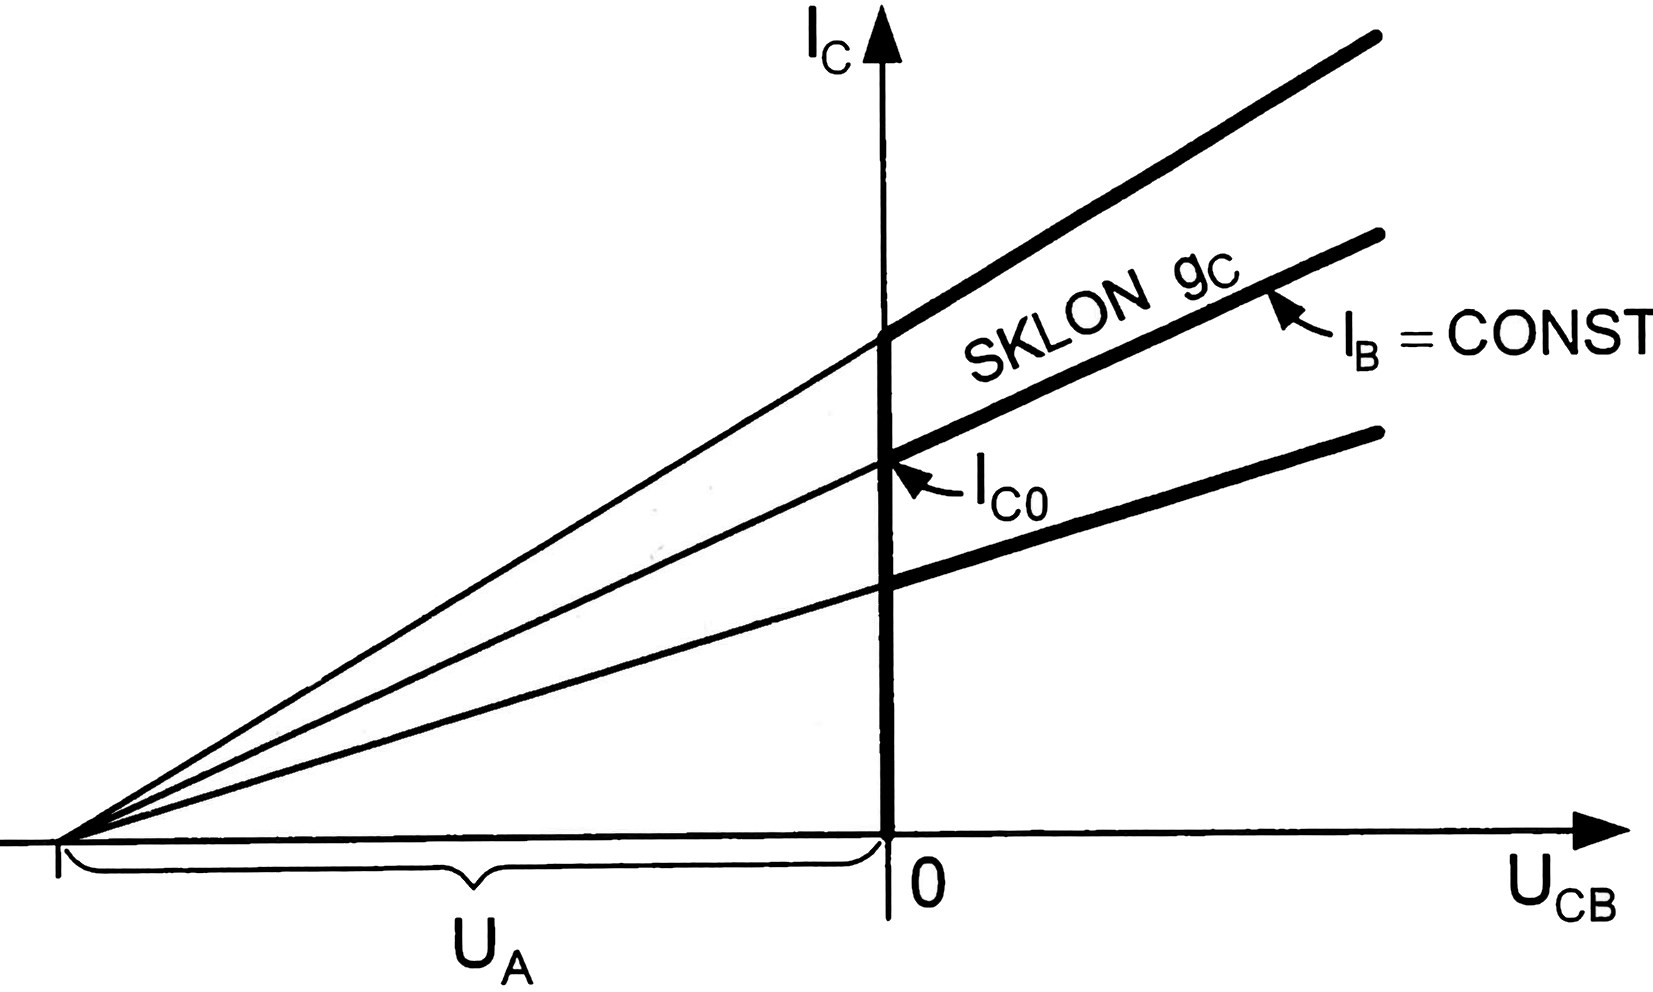
\includegraphics[width=0.6\linewidth]{aes_fig065.jpg}
          \caption{Interpretace Earlyho napětí \(U_A\) v kolektorových charakteristikách
                   \(I_C(U_{CB})\). (\cite[s.~54]{Dostal})}
          \label{aes:fig065}
        \end{figure}

        Typická velikost Earlyho napětí vstupních tranzistorů operačního zesilovače je \(U_A=
        \SI{50}{\V}\). Jinak řečeno, nasycený proud \(I_S\) a proudové zesílení \(\beta\) se
        zvětšují přibližně o \SI{2}{\percent} z výchozí hodnoty \(I_{S0}\) nebo \(\beta_0\) na každý
        \SI{1}{\V} kolektorového napětí \(U_{CB}\). Výrobní rozptyl Earlyho napětí je typicky
        \SI{50}{\percent} v souboru nevybíraných tranzistorů téhož technologického typu a
        \SI{10}{\percent} až \SI{0.1}{\percent} mezi dvěma tranzistory monolitické dvojice.

    \subsection{Unipolární vstupní stupeň}\label{aesIchIIIsecIIIssecII}
    \subsection{Konstrukční úpravy vstupního stupně}\label{aesIchIIIsecIIIssecIII}
    \subsection{Výstupní stupeň}\label{aesIchIIIsecIIIssecIV}
    \subsection{frekvenční kompenzace}\label{aesIchIIIsecIIIssecV}

%---------------------------------------------------------------------------------------------------   
  % !TeX spellcheck = cs_CZ
%---------------------------------------------------------------------------------------------------
% file opamp.tex
%---------------------------------------------------------------------------------------------------
%================================ Kapitola: Zesilovače==============================================
\setchaptertoc
\chapter{Operační obvod}\label{aesIchIV}    
  \section{Ideální operační obvod}\label{aesIchIVsecI}
    \subsection{Paralelní operační obvod}
      \fbox{Napěťový invertor} ukazuje, že vstupní signálový proud může být generován také 
      synteticky, kombinací napěťového signálového zdroje a sériového rezistoru. Takovým způsobem 
      vytvořený \emph{napěťový invertor} na obr. * je jedním z nejčastějších operačních obvodů. 
      
      Vstupní napětí $u_s$ je celé vloženo na rezistor $R_1$ (jeho pravý konec je virtuálně 
      uzemněn) a vyvolává ekvivalentní vstupní proud $\frac{u_s}{R_1}$. Tento přitékající proud je 
      kompenzován proudem $-\frac{u_0}{R_2}$ odsávaným přes zpětnovazební rezistor $R_2$ do výstupu 
      operačního zesilovače $$\frac{u_s}{R_1}=-\frac{u_0}{R_2}.$$ Ideální operační rovnice
      \begin{equation}\label{AES:eq_opamp_inv02}
        u_0 = - \frac{R_2}{R_1}u_s.
      \end{equation}
      Vyjadřuje úměrnost signálových napětí $-u_0$ a $u_s$ velikostem přilehlých rezistorů $R_2$ a 
      $R_1$. Pro snadnější zapamatování se nabízí představa dvouramenné páky s délkami ramen $R_1$ 
      a $R_2$, otočné v bodě odpovídajícímu virtuální zemi, která přenáší výchylku $u_s$ levého 
      konce na výchylku $u_0$ pravého konce v opačné polaritě.

      \begin{figure}[ht!]
        \centering
        \subcaptionbox{$u_0 = -\dfrac{R_2}{R_1}u_s, \qquad R_{\parallel} = R_1, 
                  \qquad R_{\mathsf{O}\lvert} = s0$       \label{aes:fig075a}}
          {\luafigure[0.49]{opamp_inv01a.pdf}}                                    \newline
        \subcaptionbox{ $u_0 = -\dfrac{R_2}{R_2+R_s}u_s$  \label{aes:fig075b}}
          {\luafigure[0.50]{opamp_inv01b.pdf}}             
        \caption{Napěťový invertor. Jeho mechanickou analogií je dvouramenná páka (a). Přítomnost 
                 vnitřního odporu signálového zdroje $R_s$ v operační rovnici je důsledkem 
                 konečného vstupního odporu $R_{\parallel} = R_1$ (b). }
        \label{aes:fig075}
      \end{figure}
      Zesílení napěťového invertoru 
      \begin{equation}\label{AES:eq_opamp_inv01}
        G_i = -\frac{R_2}{R_1},
      \end{equation} 
      je záporné a nastavitelné v širokých mezích od $0$ do $\infty$ výběrem rezistorů $R_1$ a 
      $R_2$. Zvláštním případem je jednotkový invertor se stejnými rezistory $R_1 = R_2$, který 
      prostě invertuje polaritu vstupního napětí: $$u_0 = - u_s, \qquad G_i = -1.$$
      
      Výstupní odpor napěťového invertoru je ideálně nulový. Jeho vstupní odpor však ztrácí onen 
      vyhranění charakter typický pro kanonické operační obvody a nabývá indiferentní velikosti 
      \begin{equation}\label{AES:eq_opamp_inv03}
        R_{\parallel} = R_1,
      \end{equation} 
      rovné velikosti virtuálně uzemněného rezistoru $R_1$.
      
      Napěťový invertor zatěžuje signálový zdroj (obr. *). To se projevuje poklesem svorkového 
      napětí signálového zdroje o úbytek na vnitřním odporu $R_s$, nebo jinak řečeno, přítomností 
      nedefinovaného a nestálého vnitřního odporu $R_s$ v operační rovnici invertoru:  
      \begin{equation}\label{AES:eq_opamp_inv04}
       u_0 = -\frac{R_2}{R_1 + R_s}u_s.
      \end{equation}      
      Taková vlastnost se obvykle považuje za nedostatek. 
            
    \subsection{Sériový operační obvod}
    
    \subsection{Složený operační obvod}
      Operační obvody, které není možné zahrnout do předcházejích dvou velkých tříd, se vyznačují:
        \begin{itemize}[noitemsep]
          \item signálovým buzením obou vstupů operačního zesilovače,
          \item násobnou zpětnou vazbou,
          \item kombinací záporné a kladné zpětné vazby,
          \item použitím několika operačních zesilovačů,
          \item nestandardním zapojením operačního zesilovače.
        \end{itemize}
      \subsubsection{Signálové buzení obou vstupů}
        \fbox{Rozdílový zesilovač} na obr. \ref{AES:fig_diff_opamp01} je lineární operační obvod se
        dvěma vstupy. Jeho výstupní napětí se najde superpozicí \cite[s.~126]{Dostal}. 
        
        Nechť působí napětí $u_1$ a napětí $u_2$ je nulové. Neinvertující vstup operačního 
        zesilovače je uzemněn přes paralelní kombinaci rezistorů $R_3$ a $R_4$. Operační obvod 
        představuje napěťový invertor a první složka výstupního napětí má velikost 
        $$-\frac{R_2}{R_1}u_1.$$
        
        Nechť působí napětí $u_2$ a napětí $u_1$ je nulové. Operační obvod představuje neinvertujcí 
        zesilovač s předřazeným děličem $R_3$ a $R_4$ a druhá složka výstupního napětí má velikost 
        $$u_2\frac{R_4}{R_3+R_4}\left(\frac{R_2}{R_1}+1\right)= 
        u_2\frac{R_2/R_1+1}{R_4/R_3+1}\cdot\frac{R_4}{R_3}.$$
        
        %------------------------------
        % image: rozdílový zesilovač
        \begin{figure}[ht!]
          \centering
          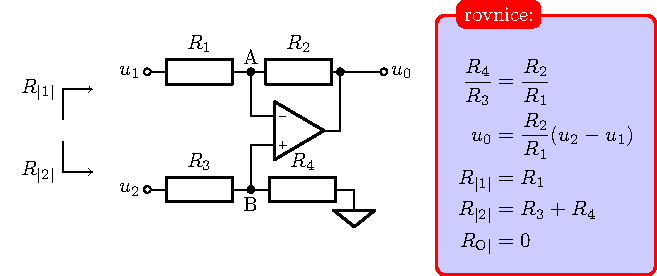
\includegraphics[width=\linewidth]{diff_opamp01.pdf}
          \caption{Rozdílový zesilovač. Podmínky potlačení souhlasné složky vstupních napětí $u_1$ a 
            $u_2$ je poměrové vyvážení zpětnovazebních rezistorů, $R_4/R_3 = R_2/R_1$. S ohledem na 
            ofset se obvykle volí uplná symetrie, tj. $R_4 = R_2$ a $R_3 = R_1$.}
          \label{AES:fig_diff_opamp01}
        \end{figure}

        Současné působení obou vstupních napětí ve vyváženém operačním obvodě
        $$\frac{R_4}{R_3}=\frac{R_2}{R_1},$$ přísluší výstupní napětí 
        \begin{equation}\label{AES:eq_diff_opamp}
          u_2 = \frac{R_2}{R_1}(u_2-u_1),   
        \end{equation}
        úměrné rozdílu vstupních napětí bez ohledu na jejich absolutní velikost. Odtud název 
        operačního obvodu. Důvod zařazení napěťového děliče ($R_3$,$R_4$) je zřejmý - dělič 
        sjednocuje zesílení invertujícího a neinvertujícího vstupu, která se liší absolutně o 
        jednotku. 
        
        Dvěma vstupům přísluší dva vstupní odpory. První vstupní odpor
        $$R_{\abs{1}} = R_1$$ je roven velikosti rezistoru $R_1$, protože vnitřní odpor bodu
        $A$\footnote{obdoba virtuální země} je nulový. Druhý vstupní odpor $$R_{\abs{2}} = R_3 +
        R_4$$ je roven součtu rezistorů $R_3$ a $R_4$, protože vnitřní odpor zbytku operačního
        obvodu v bodě $B$ je nekonečný. Tyto dva vstupní odpory jsou různé, i když jsou obě větve
        ($R_1$, $R_2$) a ($R_3$, $R_4$) stejné. 
        
        Vstupní odpory $R_{\abs{1}}$ a $R_{\abs{2}}$ přísluší dvěma samostatným uzemněným zdrojům 
        signálových napětí $u_1$ a $u_2$ podle \ref{AES:fig_diff_opamp01}. Volnému (izolovanému) 
        signálovému napěťovému zdroji připojenému diferenčně mezi vstupy rozdílového zesilovače, by 
        příslušel diferenční vstupní odpor $$R_{\abs{D}} = R_1 + R_3,$$ rovný součtové velikosti 
        rezistorů $R_{\abs{1}}$ a $R_{\abs{3}}$, protože body $A$ a $B$ jsou virtuálně zkratovány.

  \section{Analýza reálného operačního obvodu}\label{aesIchIVsecII}
  \section{Statické a dynamické chyby ve frekvenční oblasti}\label{aesIchIVsecIII}
  \section{Dynamické chyby v časové oblasti}\label{aesIchIVsecIV}
  \section{Vstupní a výstupní impedance}\label{aesIchIVsecV}
  \section{Ofset}\label{aesIchIVsecVI}
  \section{Šum}\label{aesIchIVsecVII}
  \section{Stabilita}\label{aesIchIVsecVIII}
%---------------------------------------------------------------------------------------------------
 
%=============== Kapitola: Komparátory ============================================================
  % !TeX spellcheck = cs_CZ
%---------------------------------------------------------------------------------------------------
% file opamp.tex
%---------------------------------------------------------------------------------------------------
%================================ Kapitola: Zesilovače==============================================
\setchaptertoc
\chapter{Napěťové komparátory}\label{aesIchV}  
  
  Komparátor je podobný operačnímu zesilovači. Má dva vstupy (invertující, neinvertující) a jeden
  výstup (viz \ref{aes:fig066}). Je však speciálně navržen pro porovnání napětí mezi oběma vstupy.
  Komparátor pracuje s otevřenou smyčkou a poskytuje dvoustavové logické výstupní napětí. Tyto dva
  stavy odpovídají znaménku rozdílu\footnote{včetně účinků vstupního ofsetového napětí komparátoru}
  mezi oběma vstupy.
  
  Na výstupu komparátoru bude vysoká úroveň napětí, pokud vstupní signál na neinvertujícím vstup
  převyšuje signál na invertujícím vstupu (plus ofsetové napětí, \(V_{os}\)) a nízkou úroveň pro
  opačný případ. Z hlediska terminologie používané v oblasti logických obvodů nabývá komparátor
  logickou "\texttt{1}" nebo "\texttt{0}", případně \texttt{H} (high) nebo \texttt{L} (low).
  
  Komparátor je běžně používán v aplikacích, kde je nějaká proměnná úroveň signálu porovnána s
  pevnou úrovní (obvykle referenční napětí). Protože je to ve skutečnosti \emph{1-bitový}
  analogově-digitální převodník (ADC), je komparátor základním prvkem ve všech ADC.
  (\cite[s.~72]{Vrba2000} a \cite[s.~2]{MT083}).

  \luagraphic[1]{aes_fig066.png}{Napěťový komparátor \cite[s.~1]{MT083}}{aes:fig066}

  \section{Funkce komparátoru}\label{aesIchVsecI}
    Zapojíme-li operační zesilovač podle obr. \ref{aes:fig067a}, potom se bude projevovat jeho velké
    zesílení. Je-li napájecí napětí zesilovače \SI{15}{\volt}, potom můžeme předpokládat, že
    maximální rozkmit výstupního signálu bude asi \SI{13.5}{\volt}. Meze, mezi kterými se může
    výstupní signál pohybovat jsou na převodní charakteristice uvedené na obr. \ref{aes:fig067b}
    označeny \(U_{sat}\) a \(-U_{sat}\). Velmi velká hodnota zesílení otevřené smyčky \(A_{os}\)
    činí operační zesilovač velmi citlivý na velikost rozdílu vstupních signálů.

    \begin{figure}[ht!]  %\ref{aes:fig067}
      \centering
      \subcaptionbox{\label{aes:fig067a}}{\luafigure[0.9]{aes_fig067a.png}} \\    
      \subcaptionbox{\label{aes:fig067b}}{\luafigure[0.9]{aes_fig067b.png}}                                             
      \caption{a) Zapojení operačního zesilovače bez obvodu zpětné vazby, b) převodní
              charakteristika operačního zesilovače (\cite[s.~177]{Dolecek2007})}
      \label{aes:fig067}
    \end{figure}

    Na charakteristice na obr. \ref{aes:fig067b} jsou uvedené meze výstupního signálu dosaženy již
    při velmi malých hodnotách diferenčního napětí ud na vstupu zesilovače (v příkladu uvedeném na
    obr. \ref{aes:fig067b} je výstup zesilovače v saturaci při rozdílu vstup ních napětí \(U_d =
    u_2 - u_1 = \SI{67.5}{\micro\volt}\).

    Prakticky můžeme říci, že když je \(u_2 > u_1\). bude mít napětí na výstupu zesilovače velikost
    \(U_{sat}\), když \(u_1 > u_2\), bude mít výstupní napětí velikost \(-U_{sat}\).

    \begin{tcnote}
      Doba přepnutí výstupního napětí OZ z jedné meze na druhou je omezena rychlostí přeběhu
      použitého zesilovače.
    \end{tcnote}

    Napěťový komparátor je, stejně jako operační zesilovač, \textbf{diferenční zesilovač} s velmi
    vysokým zesílením, jehož výstup nabývá pouze dva stavy. K výstupům komparátorů je možné připojit
    různá zařízení včetně různých typů logických obvodů. Z toho důvodu mají různé komparátory různá
    zapojení výstupních obvodů. Nebudeme-li uvažovat velikosti výstupních napětí a rychlosti
    spínání, můžeme uvést dvě základní zapojení výstupních obvodů:
    \begin{itemize}[noitemsep]
      \item zapojení typu \textbf{otevřený kolektor} - označení OC \emph{(open collector)};
      \item dvojčinné zapojení s \textbf{komplementárními tranzistory} - \emph{(push-pull)}.
    \end{itemize}

    \begin{figure}[ht!]  %\ref{aes:fig068}
      \centering
      \subcaptionbox{\label{aes:fig068a}}{\luafigure[0.5]{aes_fig068a.png}} \\    
      \subcaptionbox{\label{aes:fig068b}}{\luafigure[0.6]{aes_fig068b.png}} \\
      \subcaptionbox{\label{aes:fig068c}}{\luafigure[0.6]{aes_fig068c.png}}
      \caption{a) Znázornění výstupu komparátoru s otevřeným kolektorem, c) sepnutí tranzistoru, 
              když  \(u_1 > u_2\), c) tranzistor je rozepnut, když \(u_2 > u_1\) 
              (\cite[s.~177]{Dolecek2007})}
      \label{aes:fig068}
    \end{figure}

  \section{OZ ve funkci komparátoru}
    OZ jsou určeny k přesnému zesilování signálů s vysokou linearitou a stabilitou, samozřejmostí u
    nich je \emph{záporná zpětná vazba}.
    
    Stejně jako OZ se komparátory vyznačují malou vstupní napěťovou nesymetrií, velkým zesílením
    diferenčního signálu a velkým potlačením souhlasného napětí. Hlavní rozdíly mezi nimi
    spočívají v tom, že:
    \begin{itemize}[noitemsep]
      \item komparátor má logický výstup, který po překlopení do jedné ze dvou logických úrovní
            (log 1 nebo log 0) vyjadřuje, které ze dvou vstupních napětí je větší, přechod z jedné
            do druhé úrovně je velmi rychlý, ideálně skokový;
      \item OZč má analogový výstup, jeho výstupní napětí zpravidla nedosahuje mezí daných
            velikostmi napájecích napětí;
      \item OZ jsou konstruovány pro aplikace se zápornou zpětnou vazbou, nemělo by dojít k jejich
            přebuzení, které způsobí saturaci tranzistorů.
    \end{itemize}

    Komparátory jsou většinou rychlé, některé OZ rovněž. Komparátory jsou konstruovány pro velké
    vstupní diferenční signály, zatímco záporná zpětná vazba u OZ velikost diferenčních signálů
    minimalizuje. Když je OZ přebuzený, někdy i o několik \si{\mV}, některé tranzistory ve vnitřních
    zesilovacích stupních se mohou dostat do saturace. Doba zotavení nutná k přechodu ze saturace
    může trvat relativně dlouhou dobu a zesilovač je potom mnohem pomalejší než tehdy, kdy k
    saturaci nedošlo (\ref{aes:fig070}).

    \luagraphic[1]{aes_fig070.pdf}{Doba desaturace přebuzeného OZ bývá podstatně delší než jeho
                normální skupinové zpoždění (efektivně doba průchodu signálu ze vstupu na výstup)
                a často závisí na úrovni přebuzení (\emph{overdrive}).
                \cite[s.~2]{AN849}}{aes:fig070}

    \begin{tcnote}    
      Protože pouze malá skupina OZ na trhu mají uvedenou dobu zotavení pro různé úrovně přebuzení,
      je pro uživatele nezbytné stanovit tuto dobu experimentem.  Naměřené zpoždění bude záviset na
      úrovní přebuzení v dané aplikaci. Hodnota použitá při výpočtech, by měla být nejméně dvakrát
      větší než nejhorší hodnota pozorovaná testech, protože testované vzorky nemusí být
      reprezentativním vzorkem.
    \end{tcnote} 
    
    \luagraphic[0.5]{aes_fig071.pdf}{Stejná napájecí napětí umožňuje přímé buzení logického obvodu
                výstupem OZ. \cite[s.~2]{AN849}}{aes:fig071}

    Moderní OZ často mají výstupy typu rail to rail. Jejich největší kladná hodnota výstupního
    napětí se blíží k velikosti kladné hodnoty napájecího napětí, záporná hodnota se blíží k
    velikosti záporné hodnoty napájecího napětí. Když OZ a logické obvody mají stejná napájecí
    napětí, např. +\SI{5}{\volt}, je možné z výstupů OZ přímo budit následující logické obvody
    \ref{aes:fig071}. V opačném případě je nutné mezi výstupem OZ a vstupem logického obvodu vložit
    přizpůsobovací člen \cite[s.~2]{AN849} jak je tomu na obrázku \ref{aes:fig069}.
    

    \begin{figure}[ht!]  %\ref{aes:fig069}
      \centering
        \subcaptionbox{\label{aes:fig069a}}{\luafigure[0.5]{aes_fig069a.pdf}}  
        \subcaptionbox{\label{aes:fig069b}}{\luafigure[0.5]{aes_fig069b.pdf}} \\
        \subcaptionbox{\label{aes:fig069c}}{\luafigure[0.6]{aes_fig069c.pdf}}
      \caption{Přizpůsobení výstupu OZ ke vstupu logického obvodu: a) NPN, c) MOSFET N-channel, c)
                Complementary MOS inverter (\cite[s.~2]{AN849})}
      \label{aes:fig069}
    \end{figure}

    Nejjednodušší obvody rozhraní jsou \textbf{invertory}. Mohou být postaveny s NPN tranzistory,
    avšak za cenu vyšší spotřeby dané proudem báze, nebo výhodněji MOSFET s kanálem typu N.
    vytvořeny invertory s tranzistory NPN, případné s tranzistory MOSFET s kanálem typu N. 
    
    Rezistor \(R_B\) na obr. \ref{aes:fig069a} slouží k nastavení proudu báze, rezistor \(R_L\) k
    nastavení kolektorového proudu a je-li tranzistor uzavřen, zabezpečuje vstupní proud logického
    členu ve stavu log 1. Čím menší jsou velikosti odporů, tím rychlejší je činnost zapojení. NMOS
    tranzistor na obr. \ref{aes:fig069b} by měl mít malé prahové napětí \(V_{GS(th)}
    <\SI{2}{\volt}\) a také průrazné napětí hradla \(V_{GS_{max}}\) musí být větší než \(V_A\).
    Obecně musí platit, že napájecí napětí OZ \(+V_A > +V_L\) a zároveň \(-V_A < -V_L\).

    Invertor vytvořený pomocí komplementárních tranzistorů MOSFET je znázorněn na obr.
    \ref{aes:fig068c}. Jeho výhodou je malý klidový proud. Nevýhoda spočívá ve vzniku proudových
    špiček v časovém intervalu přepínání tranzistorů, kdy jsou oba tranzis tory krátkou dobu
    současně otevřeny.

    \section{Komparační úroveň a hystereze}
      \subsection{Komparační úroveň}
        
    \section{Shrnutí}
      \begin{itemize}[noitemsep]
        \item Operační zesilovač může být použit s velkou přesností jako komparátor na nízkých
              kmitočtech\footnote{Nemá smysl použít operační zesilovač jako komparátor, pokud je
              důležitá vysoká rychlost.}. Použití přesných OZ je důležité hlavně pn porovnávání
              signálů na úrovni mikrovoltů.
        \item Použití OZ může být výhodné též z cenových důvodů, když využíváme např. tři operační
              zesilovače ze čtyř umístěných v jednom pouzdru. Použití čtvrtého zesilovače jako
              komparátoru potom může být velmi ekonomické. 
        \item Pro jejich použití jako komparátorů je nutné znát rozdíly a podobnosti mezi
              komparátory a OZ, podrobně se seznámit s jejich vlastnostmi z technické dokumentace
              a to hlavně s jejich dobami zotavení, rychlostmi přeběhu, spotřebou a cenou.
        \item Komparátory jsou určeny pro rychlé rychlé spínání a v důsledku toho často mají horší
              DC parametry než mnoho operačních zesilovačů. Proto může být vhodné použít operační
              zesilovač jako komparátor v aplikacích vyžadující nízký \(V_{OS}\), nízký \(I_B\) a
              široký \(CMR\).
      \end{itemize}        

  
  \section{Aplikace}  


%---------------------------------------------------------------------------------------------------
     
%=============== Kapitola: Systémy pro digitální zpracování analogového signálů ===================
  % !TeX spellcheck = cs_CZ
{\tikzset{external/prefix={tikz/AES/}}
 \tikzset{external/figure name/.add={ch05_}{}}
%---------------------------------------------------------------------------------------------------
% file DA_AD_converter.tex
%---------------------------------------------------------------------------------------------------
%======================= Kapitola: Konverze mezi digitálním a analogový signálem====================
\chapter{Konverze mezi digitálním a analogový sig\-ná\-lem}
\minitoc

\section{Konverze mezi digitálním a analogový signálem}
  Při zpracování analogového signálu je jednou z důležitých funkcí převod tohoto signálu z analogové podoby do číslicové a naopak. Proto jsou analogově-číslicové převodníky resp. číslicově-analogové převodníky (ADC - Analog-to-Digital Converter), (DAC - Digital-to-Analog Converter) velmi důležitými prvky jakéhokoli systému zpracovávajícího signál \cite[s.~11]{Haze}. Na obrázku \ref{AES:fig_ADC_DAC_IO} je definováno rozhraní obou typů převodníku.
  \begin{figure}[ht!]
     \centering
     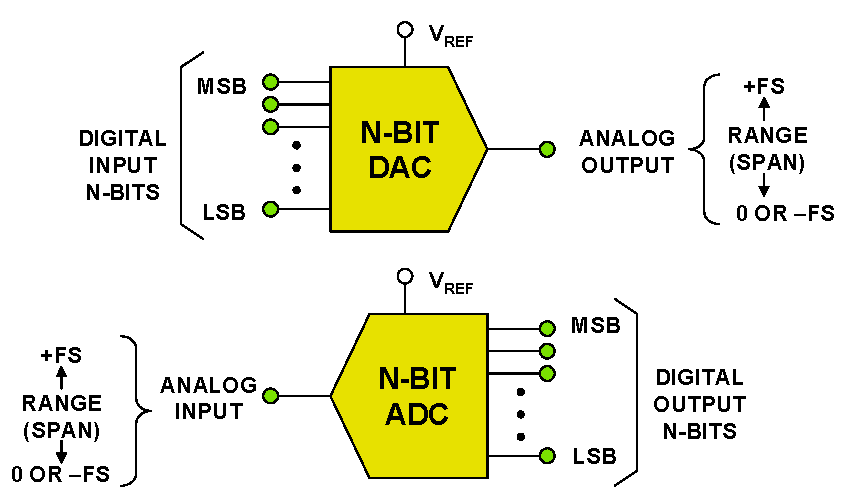
\includegraphics[width=\linewidth]{ADC_DAC_block.pdf}
     \caption[Definice I/O bloku DAC a ADC ]{Definice rozhraní bloku analogově-číslicového (ADC) a číslicově-analogového (DAC) převodníku}
     \label{AES:fig_ADC_DAC_IO}
  \end{figure}

  \textbf{Analogově-číslicové převodníky} (Analog-to-Digital Converters) slouží k pře\-ve\-de\-ní 
  analogového signálu na signál číslicový. Pro A/D převodník má analogová stupnice vstupního 
  signálu délku \texttt{FS} (\emph{Full scale}), udávanou např. ve voltech. Stupnice číslicového 
  signálu pak vyznačuje diskrétní hodnoty výstupu, které převodník generuje při převodu analogového 
  signálu \cite[s.~202]{Neumann}.

  \textbf{Číslicově-analogové převodníky} (Digital-to-Analog Converters) slouží k o\-pač\-né\-mu 
  procesu, tedy k pře\-ve\-de\-ní číslicového signálu na signál analogový, což by šlo realizovat 
  pomocí lineárního digitálního potenciometru a připojeného zdroje referenčního napětí na jeho 
  vstupu \cite[s.~208]{Neumann}. Pro N-bitové binární slovo by musel mít $n-1$ rezistorů a $n$ 
  resp. $2n - 1$ spínačů. To je monoliticky téměř nerealizovatelné již pro osmi- a vícebitové 
  slovo. Řešení převodníků proto musí být mnohem úspornější, i když úspory budou vykoupeny jinými 
  nevýhodami, případně omezeními pro jejich použití.

    \subsection{Základní struktura převodníků}
      Obě skupiny převodníků mohou typicky obsahovat komparátory, číslicové obvody, spínače, 
      integrátory, vzorkovací obvody a/nebo pasivní součástky. Nezbytnou a důležitou součástí je i 
      přesný zdroj referenčního napětí. V mnoha případech pak také platí, že DAC je jednou z částí 
      ADC.
      
      Analogově číslicový převod můžeme pomyslně rozložit do tří etap \cite{Sebesta}.
      \begin{enumerate}\addtolength{\itemsep}{-0.5\baselineskip}
        \item Převod signálu se spojitým časem na signál s diskrétním časem. Tomuto převodu říkáme  
              vzorkování.
        \item Kvantování vzorku s cílem vyjádřit vzorky konečnou množinou čísel. Tento krok je 
              provázen vznikem tzv. kvantovacího šumu. Uvedený jev souvisí s nelineárním zkreslením 
              známým z teorie obvodů.
        \item Kódování spočívající zpravidla v binárním vyjádření čísel představujících velikosti  
              vzorku.
      \end{enumerate}
      
    \subsection{Statické a dynamické parametry převodníků}
      Statické parametry převodníků jsou určovány pomocí \emph{převodní charakteristiky}, zatím co dynamické vlastnosti se vyhodnocují z kmitočtového spektra převodníku \cite[s.~11]{Haze}.
      \begin{itemize}\addtolength{\itemsep}{-0.5\baselineskip}
        \item rozsah,
        \item integrální a diferenciální nelinearita (\emph{integral - INL, differential - DNL nonlinearity}),
        \item rozlišení převodníku (\emph{resolution}),
        \item přesnost (\emph{accuracy}),
        \item chyba monotónnosti,
        \item chyba nastavení nuly (\emph{offset error}),
        \item hystereze a další.
       \end{itemize}
       K hlavním dynamickým parametrům patří
       \begin{itemize}\addtolength{\itemsep}{-0.5\baselineskip}
         \item odstup signál - šum (\emph{signal to noise ratio - SNR}) kap. \ref{AES:cap_SNR},
         \item efektivní počet bitů (\emph{effective number of bits - ENOB}),
         \item harmonické zkreslení (\emph{total harmonic distortion - THD}),
         \item odstup signál-šum a zkreslení (\emph{signal to noise and distortion - SINAD}),
         \item dynamický rozsah bez parazitních složek \newline(\emph{spurious free dynamic range 
               - SFDR}),
         \item šum - vrcholový, efektivní (\emph{noise - peak, rms}),
         \item doba přepnutí a ustálení.
       \end{itemize}

    \subsection{Vzorkování}
    \subsection{Kvantování}
       Pro přechod od časově spojitého signálu se spojitou množinou hodnot k číslicovému signálu, 
       je nutné provést (výškové) \texttt{kvantování}, tj. kvantování hodnot signálu, které je 
       patrné z obrázku \ref{AES:fig_Quntized_sig_wave}. Je zřejmé, že mapování spojitého intervalu 
       vstupních hodnot na diskrétní hodnoty digitálního výstupu způsobí, že každá hodnota 
       digitálního výstupu platí pro vstupní signál měnící se v určitém  podintervalu. Délka 
       podintervalu, pro který platí jedna hodnota digitálního výstupu se nazývá 
       \textbf{kvantizační krok převodníku} - \emph{Q}, jenž je roven bitu s nejnižší váhou - 
       \texttt{LSB}.

       \begin{figure}[ht!]
         \centering
         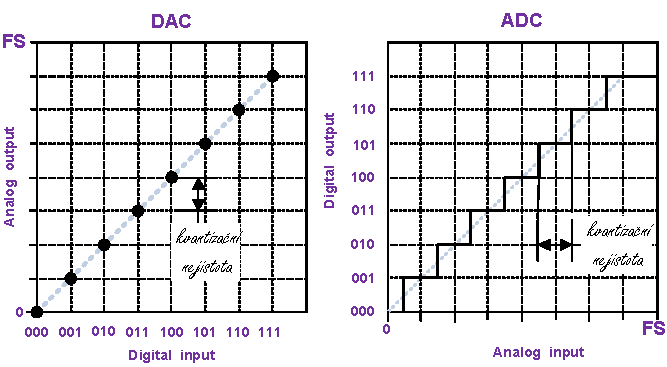
\includegraphics[width=1\linewidth]{ADC_DAC_3bit.pdf}
         \caption[Přenosová funkce AD a DA převodníku]{Ideální přenosová funkce 3bitového    
                  unipolárního AD a DA převodníku. V případě DA převodníku je přenosová funkce 
                  tvořena osmi body, nikoliv čárou.}
         \label{AES:fig_3b_DAC_ADC}
       \end{figure}
 
       Převodní charakteristika DA i AD převodníku je znázorněna na obr. \ref{AES:fig_3b_DAC_ADC}. 
       Analogový signál je spojitý a číslicový signál vyjadřuje jen jeho vybrané diskrétní hodnoty. 
       Proto je převodní charakteristika nespojitá. Naproti tomu digitální vstup vytvoří na výstupu 
       pouze omezený počet hodnot výstupního signálu.

       \begin{figure}[ht!]
         \centering
         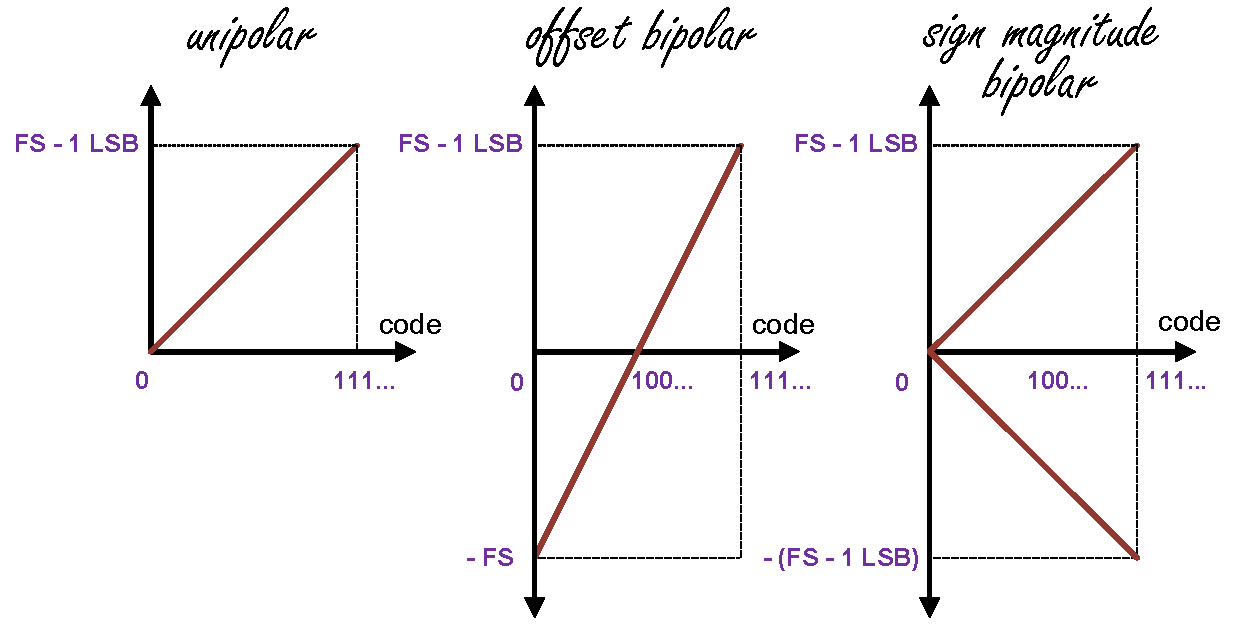
\includegraphics[width=1\linewidth]{Uni_Bi_Converter.pdf}
         \caption[Unipolární a bipolární převodníky]{Unipolární a bipolární převodníky \cite{Kester2004}}
         \label{AES:fig_uni_bi_converter}
       \end{figure}

       Počet úrovní AD převodníku, do kterého je rozdělen rozsah vstupního analogového signálu 
       definuje \textbf{rozlišovací schopnost ADC} a lze ji vyjádřit různými způsoby, jak ukazuje 
       tabulka \ref{AES:tab_10b_ADC_resolution} pro 2 až 24bitového převodníku.

         \begin{table*}[ht!]
           \centering
            \setlength{\tabcolsep}{5pt}
            \begin{tabular}{|c|c|c|c|c|c|}
              \hline
                \textbf{Rozlišení} & \multirow{2}{*}{$\mathbf{2^N}$} &  \textbf{Napětí} & 
                \multirow{2}{*}{\textbf{ppm FS}}& \multirow{2}{*}{\textbf{\% FS}}&   
                \multirow{2}{*}{\textbf{dB FS}}                                                 \\
                         N     &           &  \textbf{10V FS} &        &             &          \\
              \hline
                       2-bit   &         4 &            2.5 V & 250000 &          25 &  -12     \\
              \hline
                       4-bit   &        16 &           625 mV &  62500 &        6,25 &  -24     \\
              \hline
                       6-bit   &        64 &           156 mV &  15625 &        1,56 &  -36     \\
              \hline
                       8-bit   &       256 &          39,1 mV &   3906 &        0,39 &  -48     \\
              \hline
                      10-bit   &      1024 &          9,77 mV &    977 &       0,098 &  -60     \\
              \hline
                      12-bit   &      4096 &          2.44 mV &    244 &       0,024 &  -72     \\
              \hline
                      14-bit   &     16384 &       610 $\mu$V &     61 &       0,061 &  -84     \\
              \hline
                      16-bit   &     65536 &       153 $\mu$V &     15 &      0,0015 &  -96     \\
              \hline
                      18-bit   &    262144 &         38 $\mu$ &      4 &      0,0004 & -108     \\
              \hline
                      20-bit   &   1048576 &       9.54 $\mu$ &      1 &      0,0001 & -120     \\
              \hline
                      22-bit   &   4194304 &       2.38 $\mu$ &   0,24 &    0,000024 & -132     \\
              \hline
                      24-bit   &  16777216 &           596 nV &   0,06 &    0,000006 & -144     \\
              \hline
           \end{tabular}
           \caption[Kvantizace: Velikost LSB]{Porovnání rozlišovací schopnosti AD převodníku s  
                    různou délkou výstupního slova. Z tabulky vyplývá, že kvantizační krok 
                    24bitového ADC odpovídá velikosti úbytku na rezistoru $2,2 k\Omega$ při teplotě 
                    25°C, který vzniká vlivem tepelného šumu (viz Johnsonův šum) jenž je při šířce 
                    pásma 10 kHz roven 600 nV. }
           \label{AES:tab_10b_ADC_resolution}
         \end{table*}

       \begin{figure}[ht!]
         \centering
         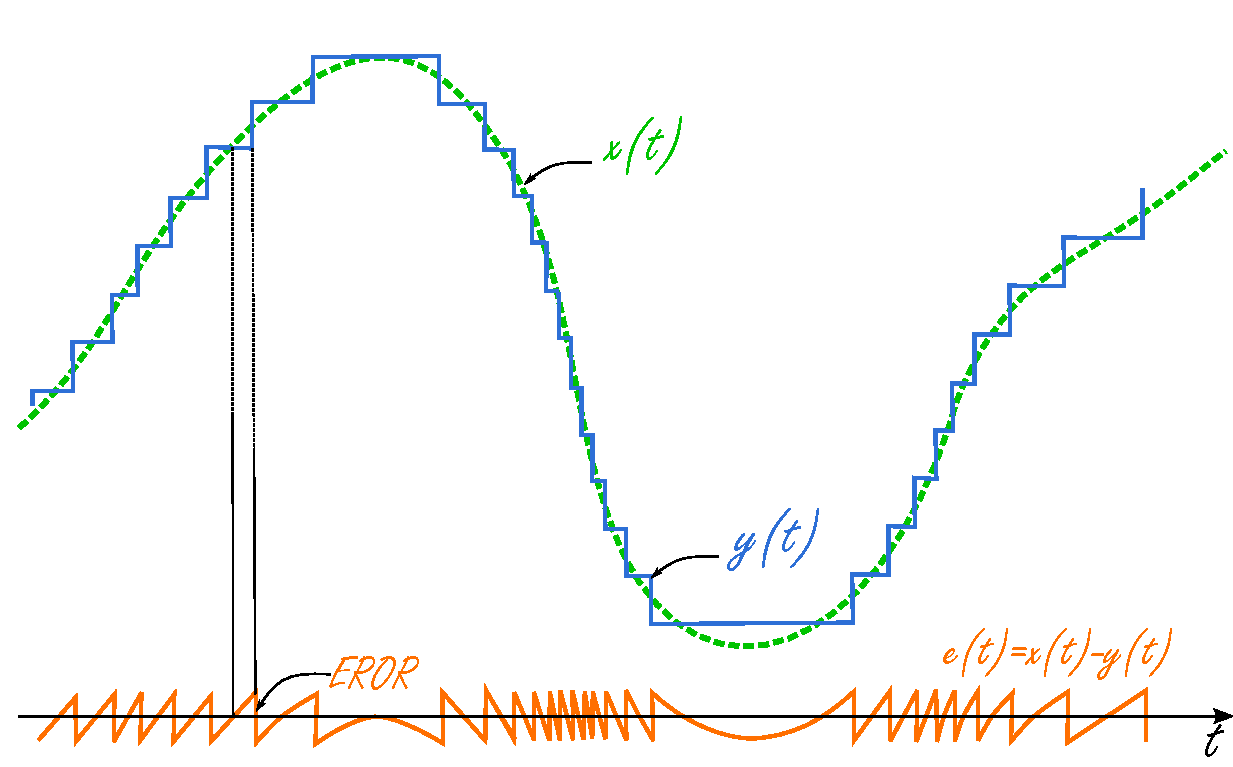
\includegraphics[width=1\linewidth]{Quantized_signal_wave.pdf}
         \caption[Kvantizační chyba]{Kvantizační chyba je rovna rozdílu původního x(t) a kvantovaného signálu v úrovni y(t) \cite{Bennett}}
         \label{AES:fig_Quntized_sig_wave}
       \end{figure}

       %The quantization error for any ac signal which spans more than a few LSBs can be 
       %approximated by an uncorrelated sawtooth waveform having a peak-to-peak amplitude of q, the 
       %weight of an LSB. Although this analysis is not precise, it is accurate enough for 
       %most applications. W. R. Bennett of Bell Laboratories analyzed the actual spectrum of 
       %quantization noise in his classic 1948

       Kvantizační chyba, jejíž průběh je na obr. \ref{AES:fig_Quntized_sig_wave}, v dynamickém 
       režimu, tj. při časových změnách vstupní analogové veličiny, způsobuje \textbf{kvantizační 
       šum}. Ten lze pozorovat např. tehdy, kdy čísla získaná z převodníku A/D jsou vedena do 
       převodníku D/A a jím je analogový signál rekonstruován. Rekonstruovaný signál se jeví jako 
       signál původní, avšak se superponovaným rušivým signálem. Vzájemným odečtení 
       rekonstruovaného a původního signálu, dostaneme samostatný rušivý signál, který lze podrobit 
       analýze. \emph{Pokud je vzorkovací signál nekorelovaný se vzorkovaným signálem, je možno 
       kvantizační šum považovat za náhodný}. Vztah mezi původním signálem a signálem degradovaným 
       kvantizačním šumem vyjadřuje parametr - \texttt{SNR}
       \begin{itemize}
         \item SNR  - Signal to Noise Ratio: poměr signálu k šumu
             \begin{equation}\label{AES:eq_SNR}
                SNR = \frac{E\{x^2(t)\}}{E\{[y(t)-x(t)]^2\}}
             \end{equation}
                \begin{itemize}
                   \item $E\{.\} \cdots$ operátor průměrování
                   \item $x(t)   \cdots$ vstupní analogový signál
                   \item $y(t)   \cdots$ rekonstruovaný kvantovaný signál
                 \end{itemize}
       \end{itemize}
       Kvantizační chybu lze aproximovat nekorelovaným pilovým průběhem s amplitudou špička-špička 
       rovnou kvantizačnímu kroku $Q$. Ačkoliv takto provedená analýza (viz kapitola 
       \ref{AES:kap_kv_sum}) není přesná, v běžných aplikacích zcela postačuje.

       Na obr. \ref{AES:fig_AD_kvantizacni_chyba} je kvantování realizováno tak, že je zajištěna 
       minimální chyba kvantování, tj. převodník provádí operaci zaokrouhlování na nejbližší 
       hodnotu. To znamená, že např. číslo jedna bude generováno vstupem v intervalu $1\pm0,5V$, 
       je-li \texttt{FS} rovno 8V a máme-li k dispozici osm kvantizačních úrovní.

       Převodník, který má v celém intervalu předváděných vstupních hodnot konstantní kvantizační 
       krok, se též označuje jako lineární kvantizér. Převodník s přirozeným binárním kódem o 
       \emph{N} bitech je schopen na analogové straně reprezentovat \emph{n-1} ne\-nu\-lo\-vých 
       úrovní analogové veličiny, přičemž platí
       \begin{equation}\label{AES:eq_AD_kod}
          n = 2^N
       \end{equation}
       A jde-li o lineární N-bitový kvantizér, můžeme vyjádřit kvantizační krok vztahem
       \begin{equation}\label{AES:eq_kvant_krok}
          Q = \frac{FS}{n} = \frac{FS}{2^N}
       \end{equation}
       Nejvyšší úroveň vstupní veličiny \emph{A} pak bude
       \begin{equation}\label{AES:eq_A_max}
          A_{max} = \frac{n-1}{n}+\frac{Q}{2}
       \end{equation}

       V sekvenci bitů binárního čísla generovaného převodníkem se zpravidla první bit, který představuje nejvyšší binární řád, označuje \texttt{MSB} (\emph{Most Significant Bit}), tedy nejvýznamnější bit. Poslední bit, tj. bit v poloze nejnižšího řádu, má označení \texttt{LSB} (\emph{Least Significant Bit}), tedy nejméně významný bit. Je zřejmé, že \texttt{LSB} jednoznačně určuje základní krok na ose číslicového signálu. Dojde-li ke změně pouze v hodnotě \texttt{LSB}, změní se analogová hodnota právě o kvantizační krok. \texttt{LSB} tedy na analogové straně určuje rozlišovací schopnost převodníku. Např. osmibitový převodník má rozlišovací schopnost \texttt{FS/256}, tj. přibližně \texttt{0,4\%}. Je-li \texttt{FS = 2V}, musí rozlišit \texttt{8 mV}\cite[s.~203]{Neumann}.

       Vzhledem k diskretizaci hodnot původního analogového signálu při převodu A/D dochází ke \emph{kvantizačním chybám}. Je-li např. vstupní veličinou okamžité napětí $u_a$ a této hodnotě odpovídá na výstupu číslo $D$, pak kvantizační chybu $\varepsilon_q$ lze vyjádřit takto:
       \begin{equation}\label{AES:eq_kvant_chyba}
          \varepsilon_q = u_a - FS\frac{D}{2^N}
       \end{equation}

      \subsection{Kvantizační šum ideálního N-bitového ADC}\label{AES:kap_kv_sum}

      %The only errors (dc or ac) associated with an ideal N-bit data converter are those related  
      %to the sampling and quantization processes. The maximum error an ideal converter makes when 
      %digitizing a signal is $\pm 1/2 LSB$. The transfer function of an ideal N-bit ADC is shown 
      %in Figure 2.37. The quantization error for any ac signal which spans more than a few LSBs 
      %can be approximated by an uncorrelated sawtooth waveform having a peak-to-peak amplitude of 
      %q, the weight of an LSB.

      %The quantization error for any ac signal which spans more than a few LSBs can be 
      %approximated by an uncorrelated sawtooth waveform having a peak-to-peak amplitude of q, the 
      %weight of an LSB. Although this analysis is not precise, it is accurate enough for most 
      %applications. W. R. Bennett of Bell Laboratories analyzed the actual spectrum of 
      %quantization noise in his classic 1948

      V předchozí kapitole byla nastíněna možnost aproximace kvantizační chyby jaké\-ho\-koliv AC 
      signálu v časové oblasti (viz \ref{AES:fig_Quntized_sig_wave}) nekorelovaným pilovým 
      průběhem, za cenu určité nepřesnosti vyvážené jednodušším matematickým aparátem.

      Vyjděme tedy z převodní charakteristiky ideálního N-bitového převodníku zatížené kvantizační 
      chybou, tak jak je znázorněna na obr. \ref{AES:fig_AD_kvantizacni_chyba}. Z té je patrné, že 
      chyba může v absolutní hodnotě dosáhnout maximálně $e(t) = \frac{Q}{2}$, resp. 
      $\pm\frac{1}{2}LSB$ a v rámci kvantizačním kroku ji lze popsat přímkou se strmostí 
      \texttt{s}: $$e(t) = st, -\frac{Q}{2s}<t<+\frac{Q}{2s}.$$ Statisticky je pravděpodobnost 
      jejího rozložení 1/Q a je rovnoměrná od $-\frac{Q}{2}$ do $+\frac{Q}{2}$.

      \begin{figure}[ht!]
        \centering
        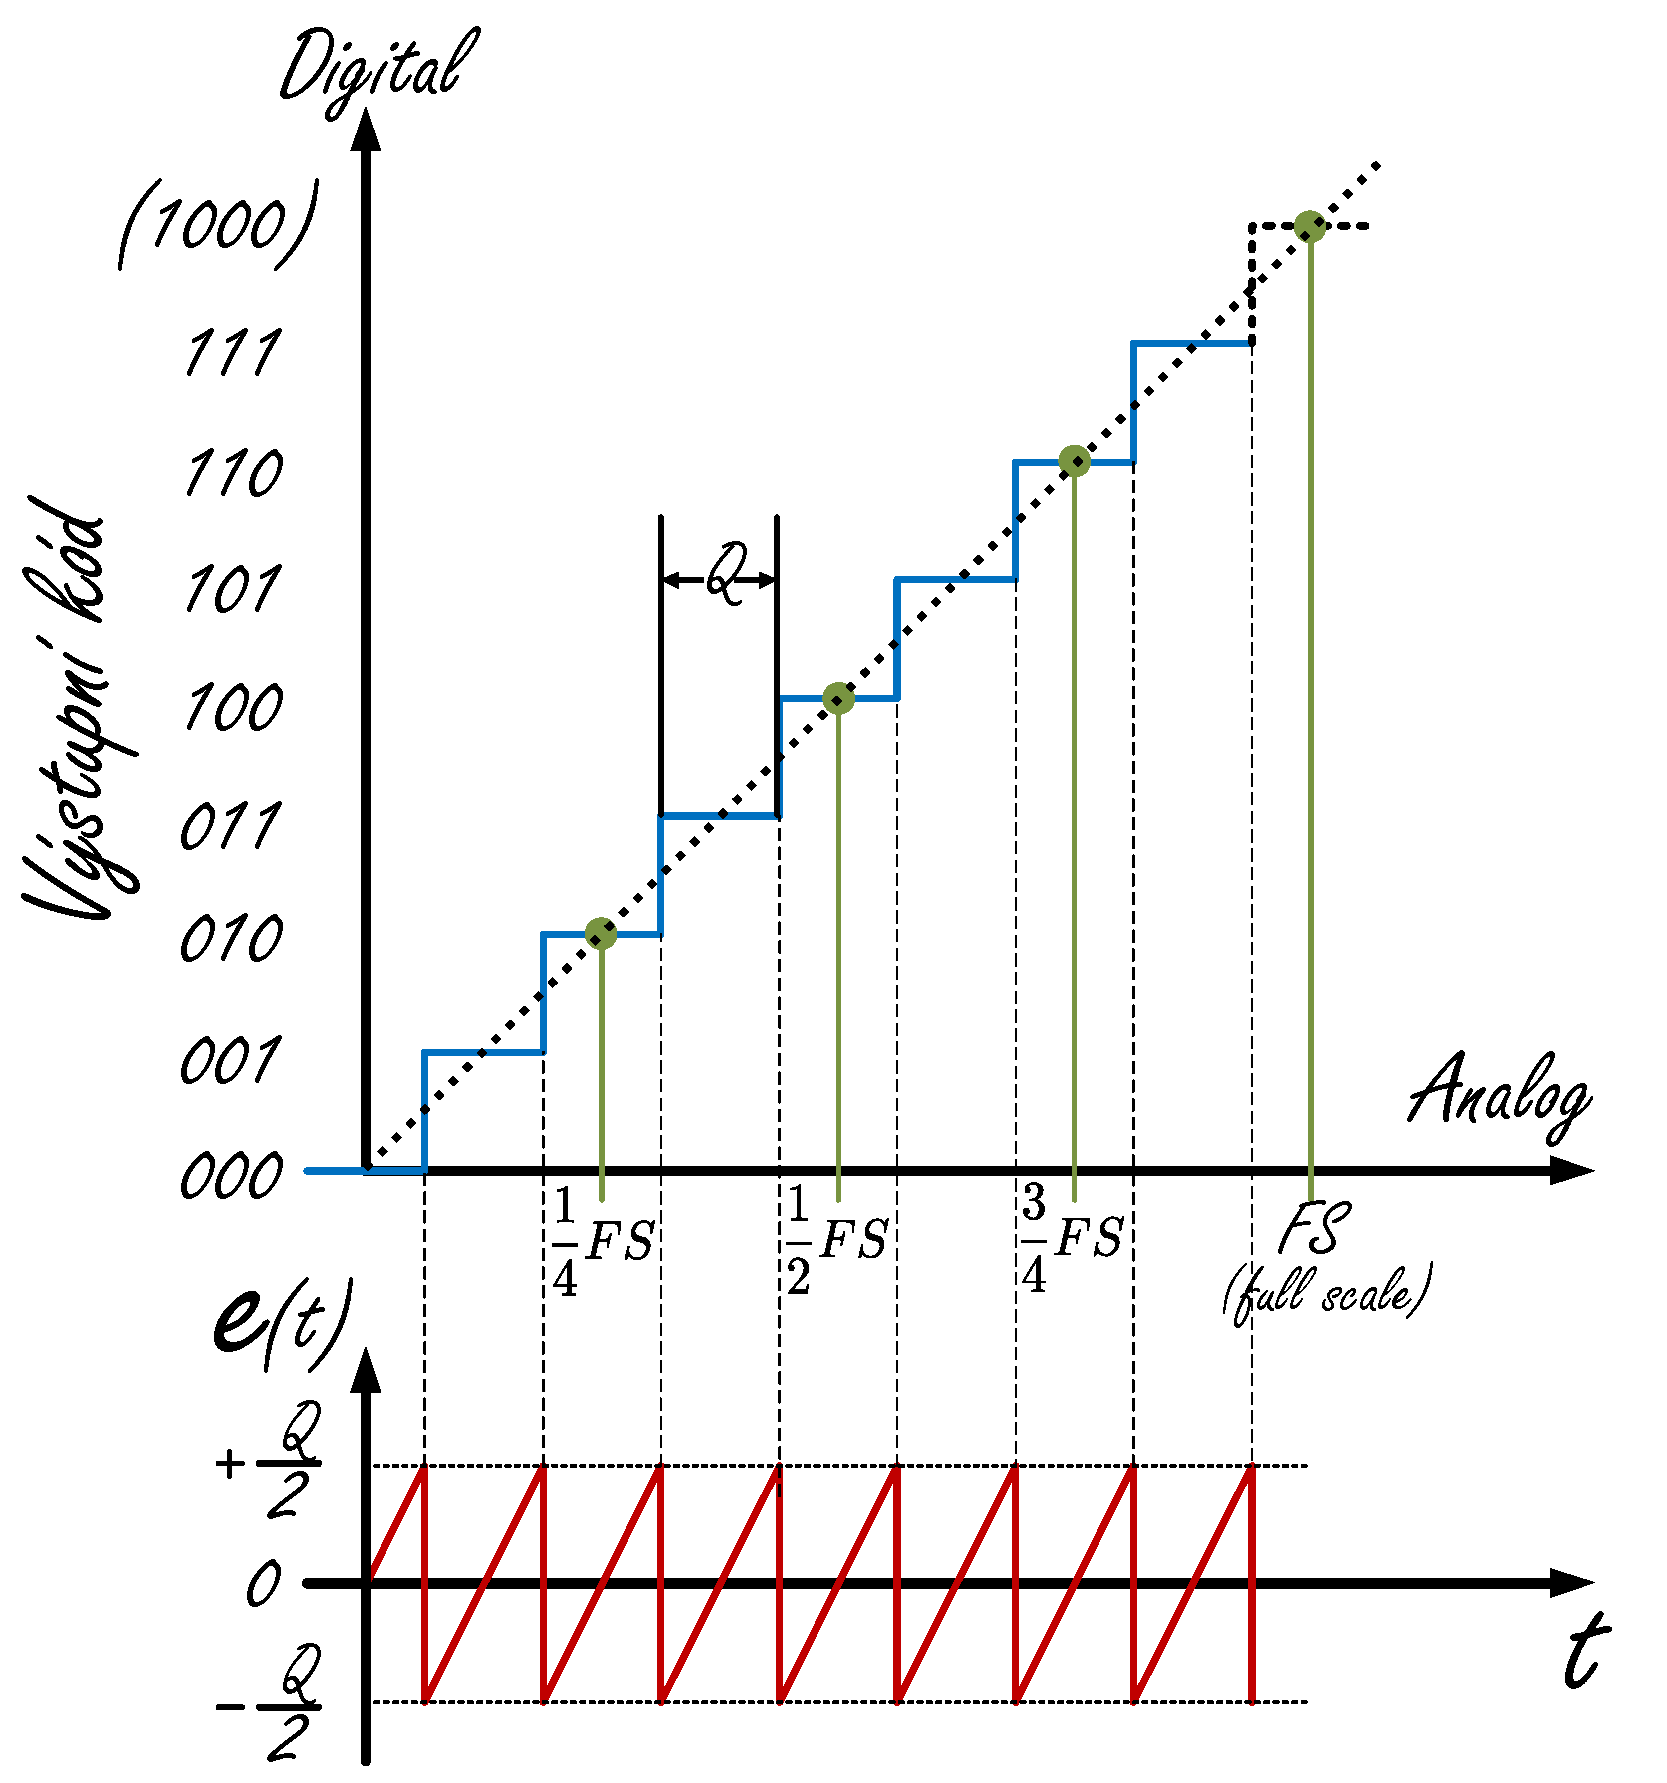
\includegraphics[width=0.8\linewidth]{AD_kvantizacni_chyba.pdf}
        \caption[Převodní charakteristika ideálních převodníků]{Převodní charakteristika 
                 ideálních převodníků a závislost chyby kvantizace na vstupní analogové hodnotě}
        \label{AES:fig_AD_kvantizacni_chyba}
      \end{figure}

      Z výše uvedeného plyne, že okamžitá hodnota kvantizační chyby $\varepsilon_q(t) = y(t) - x(t)$ může dosáhnout rozkmitu maximálně $\pm \frac{Q}{2}$ a jelikož předpokládáme rovnoměrné rozložení hodnot, je hustota pravděpodobnosti amplitud rovna $\frac{1}{Q}$.

      \emph{Kvantizační šum $\sigma^2$ je definován jako výkon (rozptyl) střídavé složky kvantizační chyby $\varepsilon_q$ a jeho efektivní hodnotu $\sigma$ můžeme odvodit pomocí věty o druhém centrálním momentu nebo výpočtem efektivní hodnoty v časové oblasti.}

        \begin{figure}[ht!]
          \centering
          \subfloat[Hustota pravděpodobnosti kvantizačního šumu]{\label{AES:fig_kvant_sum1}
            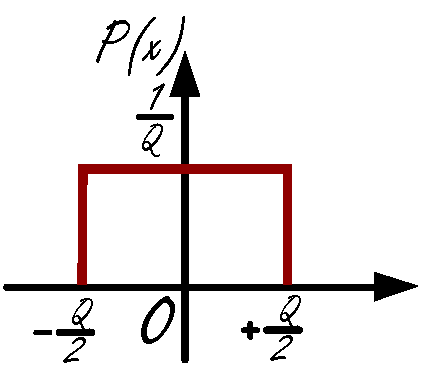
\includegraphics[width=0.4\linewidth]{AD_kvantizacni_sum1.pdf}}
          \subfloat[Kvantizační šum jako funkce času]{\label{AES:fig_kvant_sum2}
            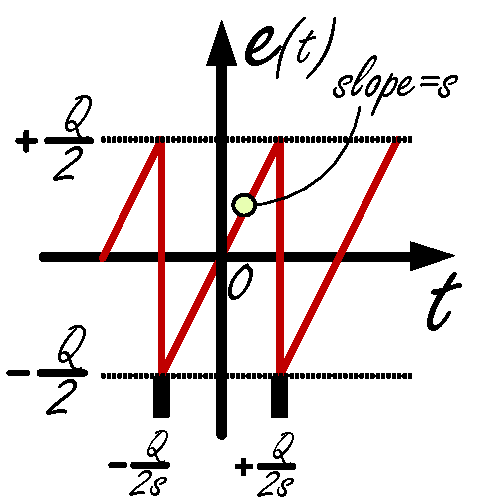
\includegraphics[width=0.4\linewidth]{AD_kvantizacni_sum2.pdf}}
          \caption{K odvození efektivní hodnoty kvantizačního šumu}
          \label{AES:fig_kvant_sum}
        \end{figure}

        \begin{enumerate}
          \item V pravděpodobnostním počtu je K-tý moment definován jako: 
                \begin{align*}
                  M_k  &= \int_{-\infty}^{\infty} x^k p(x)dx  \\
                  \shortintertext{tedy}                       \\
                  e(t) &= \int_{-\frac{Q}{2}}^{+\frac{Q}{2}}(x - x_0)^2p(x)dx = 
                                 \frac{1}{Q}\int_{-\frac{Q}{2}}^{+\frac{Q}{2}}x^2dx = \frac{Q^2}{12}
                \end{align*}
          \item V časové oblasti má kvantizační šum pilový průběh viz obr.    
                \ref{AES:fig_kvant_sum2}. Z  definičního integrálu efektivní hodnoty dostaneme $$ 
                \overline{e^2(t)} =               
                \frac{s}{Q}\int_{-\frac{Q}{2}}^{+\frac{Q}{2}}(st)^2dt = \frac{Q^2}{12}.$$ Též 
                můžeme využít znalosti efektivní hodnoty pro průběh tohoto typu: 
                $\frac{U_m}{\sqrt{3}}$ a dosazením za $U_m =\frac{Q}{2}$ získáme opět stejný 
                výsledek jako při výpočtu integrálu
        \end{enumerate}

        Tedy efektivní hodnota kvantizačního šumu ideálního N-bitového převodníku je:
        \begin{equation}\label{AES:eq_ef_kv_sumu}
            e(t) = \frac{Q}{\sqrt{12}}
        \end{equation}
        Předpokládejme na vstupu převodníku ustálený harmonický signál o amplitudě $X$. Dále 
        předpokládejme, že signál s amplitudou $X_m$ by pokryl celý rozsah převodníku $FS$. Pak se 
        dá ze vztahu \ref{AES:eq_SNR} vyjádřit odstup signálu od šumu \texttt{SNR} ideálního 
        \emph{N-bitového} převodníku jako podíl jejich výkonů resp. kvadrátu efektivních hodnot 
        signálu a šumu v decibelech vztahem
        \begin{align*}
          SNR      &= \frac{P_{signal}}{P_{noise}} =     
                      \left(\frac{A_{signal}}{A_{noise}}\right)^2         \\
          SNR_{dB} &= 10\log\frac{P_{signal}}{P_{noise}} =       
                      10\log\left(\frac{A_{signal}}{A_{noise}}\right)^2   \\
                   &= 20\log\frac{A_{signal}}{A_{noise}}                  
        \end{align*}
        \begin{equation}\label{AES:eq_SNR_N}
            SNR  = 1,76 + 6,02N + 20log\left(\frac{X}{X_m}\right)
        \end{equation}

        Lze tedy říci, že každý bit navíc v digitálním výstupu A/D převodníku přinese zlepšení 
        odstupu signálu od šumu o \texttt{6 dB}. Naproti tomu je třeba vědět, že uvedený výraz 
        počítá s harmonickým signálem různého rozkmitu. Při zmenšování amplitudy bude relativní 
        podíl šumu v signálu vyšší. Poměry se také mohou velmi změnit, když signál nebude mít 
        harmonický charakter.

      \subsubsection{Odstup signálu od šumu}\label{AES:cap_SNR}
        Z předchozí kapitoly víme, že SNR je definován jako poměr výkonu signálu k výkonu šumu ($v\acute{y}kon = ef. hodnota^2$). Pro samotný kvantizační šum platí:
        \begin{align}
          SNR_{dB} &= 10\log\left(\frac{\dfrac{2^N}{2\cdot\sqrt{2}}\cdot     
                                        Q}{\dfrac{Q}{\sqrt{12}}}\right)^2          \nonumber \\
                   &= N20\log2 + 20\log\frac{\sqrt{12}}{2\cdot\sqrt{12}}           \nonumber \\ 
          SNR_{dB} &= 6,02\cdot N + 1,76dB
        \end{align}

        \begin{figure}[ht!]
            \centering
            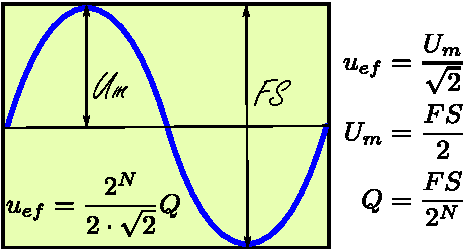
\includegraphics[width=0.6\linewidth]{AD_SNR.pdf}
            \caption{}
            \label{AES:fig_SNR}
        \end{figure}

        Tato hodnota platí pouze pro ideální převodník pouze s kvantizační chybou, a sinusový 
        signál s rozkmitem přes celý rozsah převodníku.  Skutečný převodník má ovšem vlivem dalších 
        chyb \texttt{SNR} menší než \texttt{SNR} určený pouze pro kvantizační šum. Tato hodnota se 
        nazývá \texttt{SINAD} nebo \texttt{SNDR} - \emph{Signal-to-Noise and Distortion ratio}.

        Známe-li \texttt{SNR} skutečného převodníku, můžeme určit počet efektivních bitu $N_{ef}$ 
        tzn. \emph{efektivní rozlišitelnost převodníku}. Ten je vždy menší než $N$.
        \begin{equation}\label{AES_eq_N_ef}
            N_ef = \frac{SNR - 1,76}{6,02}
        \end{equation}
        
  \section{Principy A/D převodníků}
      Převod analogového signálu na číslo lze uskutečnit několika různými postupy:\cite{Neumann}
      \begin{enumerate}
        \item Vstupní signál se porovnává s kvantovanou referenční veličinou a komparátory okamžitě 
              vyhodnotí, který z nich je větší. Přímým výstupním údajem je binární číslicové slovo.
        \item Vstupní signál i referenční veličina se v určité časové sekvenci zavádějí do   
              integrátoru a komparátor na jeho výstupu určuje sekvenci impulsů, vypovídající o 
              hodnotě vstupní analogové veličiny. Informací o vstupní veličině dále přenáší počet 
              impulsu, jejich kmitočet nebo kódovaná sekvence impulsů. Tato informace může být 
              převedena číslicovým blokem (obvykle blokem DSP) na binární číslicové slovo.
      \end{enumerate}

      Bývá také používáno třídění na \emph{převodníky s přímým a nepřímým vyhodnocení analogové 
      veličiny}.
      \begin{itemize}
        \item \texttt{Převodníky s přímým vyhodnocením} porovnávají hodnoty analogové veličiny s  
              vybranými kvantizačními úrovněmi současně nebo postupně, a to tak, že každá úroveň má 
              vlastní komparátor. K těmto převodníkům patří \emph{převodníky paralelní a kaskádní}.
        \item \texttt{K nepřímému převodu} můžeme využít postupného provoláváním vstupní  
              ve\-li\-či\-ny s vhodnými vzorky referenčního napětí, dodávanými na vstup jediného 
              komparátoru v pořadí a velikosti řízené logickými obvody. U těchto převodníků je 
              vstupní analogová veličina porovnávaná s výstupní veličinou převodníku \texttt{D/A}, 
              přičemž je číslicový vstup tohoto převodníku měněn tak, aby se obě veličiny k sobě 
              přibližovaly. Pokud se k sobě dostatečně přiblíží, je převod ukončen. I zde jsou v 
              podstatě jen dvě jednoduché možnosti přibližování výstup převodníku \texttt{D/A} k 
              určité úrovni vstupní veličiny: buď se přibližování děje se stálým krokem, kdy jde o 
              krokování po jednotlivých kvantovacích úrovních (\emph{převodníky sledovací}), nebo 
              postupnou aproximací (\emph{převodníky aproximační}), kdy první krok rozhoduje o 
              hodnotě \texttt{MSB}, další kroky porovnávají binárně zmenšované hodnoty 
              odpovídající jednotlivým binárním řádům s tím, že poslední krok určí hodnotu \texttt{LSB}.
        \item Jinou možností nepřímého převodu A/D je převést hodnotu vstupní veličiny na takový  
              parametr pomocného signálu, který se pak dá snadno převést na číslicový údaj. Tímto 
              parametrem je nejčastěji kmitočet, jindy to může být i počet impulzů v určitém 
              časovém intervalu nebo kódovaná sekvence impulzů. U těchto převodníků j kromě 
              komparátoru typickým funkčním blokem integrátor.
      \end{itemize}

  \section{Převod číslicového signálu na analogový}
    Číslicově-analogové převodníky převádějí číslicový signál zpravidla ve formě binárně kódovaného čísla na proud nebo napětí.
    \begin{equation}\label{AES_eq_DA}
        U_A = D \cdot U_{REF} \quad  I_A = D \cdot I_{REF}
    \end{equation}
    kde $U_{REF}, I_{REF}$ jsou referenční napětí a proud určující rozsah výstupní veličiny. Je-li 
    referenční napětí konstantní jedná se o klasické převodníky \texttt{DAC}. Při proměnném 
    referenčním napětí se jedná o násobící převodníky \texttt{MDAC}, které realizují násobení 
    časově proměnného referenčního spojitého a vstupního číslicového signálu.  Hodnota číslicového 
    signálu $D$ se vyjadřuje ve dvojkovém nebo dvojkově desítkovém (\texttt{BCD}) kódu.
    Ve dvojkovém kódu:
    \begin{equation}\label{AES:eq_DA_Dbin}
        D_B =\sum_{i=1}^n a_i\cdot2^{-i}
    \end{equation}
    $n$ je počet bitů dvojkového čísla. Bit $a_1$ s nejvyšší vahou $1/2$ se označuje \textbf{MSB}, 
    bit  $a_n$ s nejnižší vahou $2^{-n}$  se označuje \textbf{LSB}. \emph{Maximální hodnota 
    číslicového signálu $D_{MAX} = 1 - 2^{-n}$ a proto maximální hodnota výstupní veličiny je vždy 
    o 1 LSB menší, než je rozsah převodníku.} Veličina $2^{-n}\cdot U_{REF}$, resp. $2^{-n}\cdot 
    I_{REF}$ se nazývá \textbf{kvantum referenčního napětí nebo proudu} a určuje 
    \textbf{rozlišitelnost} převodníku. Převodní funkci D/A převodníku můžeme v případě 
    binárního kódu vyjádřit vztahem
    \begin{equation}\label{AES:eq_DA_bin}
        U_A = U_{REF}\cdot\left(a_{n}2^{-n} + a_{n-1}2^{-(n-1)} + \cdots + a_12^{-1}\right)
    \end{equation}
    Statické vlastnosti \texttt{D/A} převodníku jsou určeny převodní charakteristikou, která je 
    obvykle lineární (obr. \ref{AES:fig_DA_prevodni_charka}). Převodní charakteristika reálného DA 
    převodníku je zatížena chybou nuly, chybou zisku, integrální a diferenciální nelinearitou a 
    monotónností převodu.

    Z převodní charakteristiky lze tedy určit následující parametry převodníku:
    \begin{itemize}
      \item Chybu nuly (posunu) $\varepsilon_0$
           \begin{equation}\label{AES_eq_chyba_nuly}
             \varepsilon_0 = \frac{\Delta U_0}{U_{REF}}
           \end{equation}
      \item Chybu měřítka (zesílení) $\varepsilon_m$
           \begin{equation}\label{AES_eq_chyba_zesileni}
             \varepsilon_m = \frac{\Delta U_m - \Delta U_0}{U_{REF}}
           \end{equation}
      \item Integrální nelinearitu $I_{NL}$ jako maximální odchylku výstupního napětí sku\-teč\-né\-ho 
      převodníku od ideální hodnoty v celém rozsahu převodníku
           \begin{equation}\label{AES_eq_chyba_integralni}
             I_{NL} = \frac{\max\Delta U_n}{U_{REF}}
           \end{equation}
    \end{itemize}

    \begin{figure}[ht!]
       \centering
       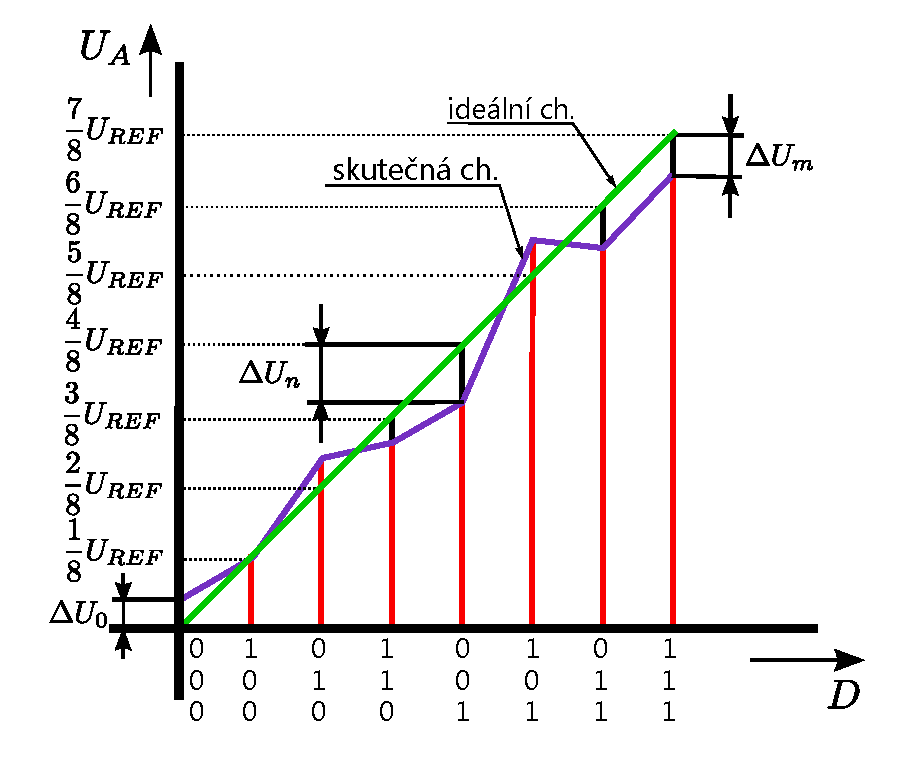
\includegraphics[width=0.8\linewidth]{DA_prevodni_charka.pdf}
       \caption[Převodní charakteristika DA převodníku]{Statická převodní charakteristika 3 bitového DA převodníku}
       \label{AES:fig_DA_prevodni_charka}
    \end{figure}

    Všechny tyto chyby se vyjadřují buď v procentech jmenovitého rozsahu $U_{REF}$ 
    pře\-vod\-ní\-ku, nebo v jednotkách ideální kvantizační úrovně (kvanta) $q = 2^{-n}\cdot 
    U_{REF}$.

    Dynamické vlastnosti D/A převodníku jsou charakterizovány \textbf{dobou ustálení} $T_u$ (obr. 
    \ref{AES:fig_DA_Tu}), potřebnou k ustálení výstupního signálu na jmenovitou hodnotu se zadanou 
    chybou $\Delta U$ obvykle $\pm0.5 LSB$.

    U násobících D/A převodníků se navíc určuje kmitočtový rozsah referenčního napětí kmitočtem 
    $f_m$, při kterém poklesne výstupní napětí převodníku o $3 dB$ oproti stejnosměrnému napětí při 
    maximální hodnotě číslicového signálu.

    \begin{figure}[ht!]
       \centering
       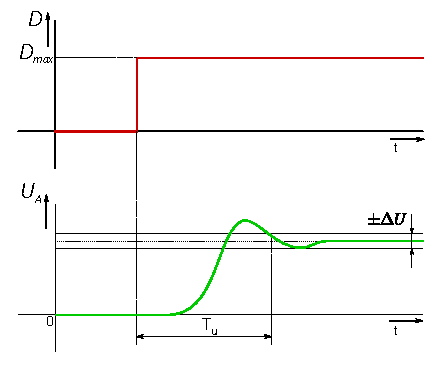
\includegraphics[width=0.4\textwidth]{DA_doba_Tu.pdf}
       \caption[Doba ustálení DA převodníku]{Doba ustálení $T_a$ DA převodníku. Je to celková   
                doba od změny vstupního kódu do ustálení analogového výstupu s přesností 
       $\pm\frac{1}{2}LSB$}
       \label{AES:fig_DA_Tu}
    \end{figure}

    \subsection{DA převodník DAC0800}
      D/A převodník DAC0800 je velmi rychlý násobící D/A převodník s rozlišením 8 bitů, pracující 
      na principu spínaných proudových zdrojů (viz obr. \ref{AES:fig_DAC0800_blok_sch}).
      \begin{figure}[ht!]
        \centering
        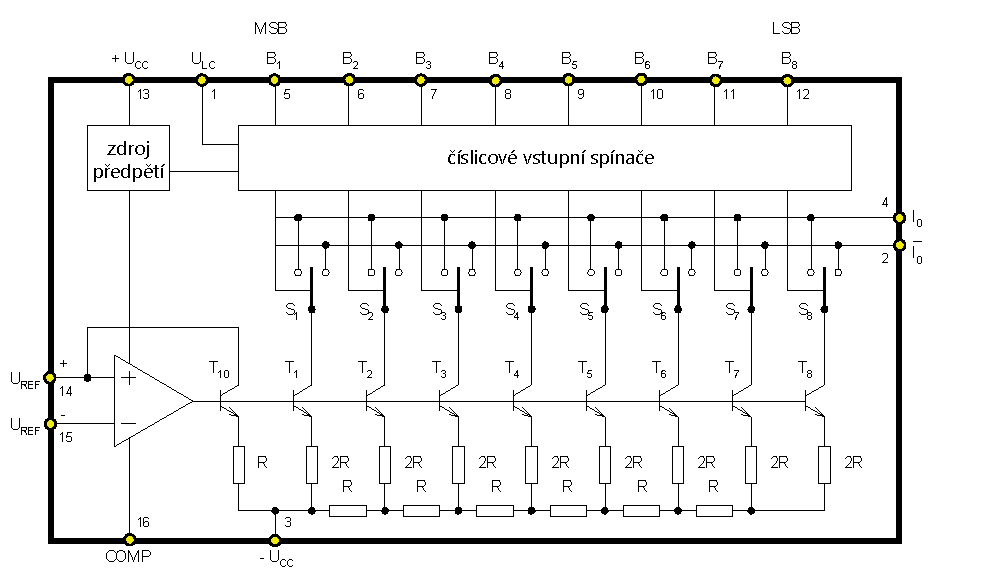
\includegraphics[width=1\linewidth]{DAC0800_block_diagram.pdf}
        \caption[Blokové schéma DAC0800]{Blokové schéma DA převodníku DAC0800}
        \label{AES:fig_DAC0800_blok_sch}
      \end{figure}

      Vstup převodníku je proudový, proudový výstup je řešen jako komplementární. IO v sobě slučuje 
      proudové spínače, váhové odpory a řídící zesilovač. Analogová reference, přesné vnější 
      odpory, korekční kondenzátor a výstupní zesilovač se připojují vně převodníku. Převodník 
      \texttt{DAC0800} generuje váhové proudy do komplementárních proudových sběrnic $I_0$ a 
      $\overline{I}_0$ prostřednictvím spínaných proudových zdrojů s tranzistory $T_1$ až $T_8$ a 
      odporovou sítí $R-2R$ viz obr. \ref{AES:fig_DAC0800_blok_sch}. Při úrovni \texttt{H} na 
      číslicových vstupech $B_1$ až $B_8$ připojí spínače $S_1$ až $S_8$ příslušné váhové proudy na 
      výstup $I_0$ a při úrovni \texttt{L} na výstup $\overline{I}_0$.

      Nezávislost váhových proudů na teplotních změnách zajišťuje referenční zdroj prou\-du s 
      tranzistorem $T_{10}$ a zesilovačem \texttt{Z}, ke kterému se připojuje referenční proud o 
      jmenovité hodnotě $2 mA$. Kondenzátor s kapacitou $10 nF$ připojený mezi vývody \texttt{3} a 
      \texttt{16} slouží ke kmitočtové kompenzaci zesilovače \texttt{Z}. Číslicové vstupy $S_1$ až 
      $B_8$ řídí spínače $S_1$ až $S_8$ prostřednictvím převodníku úrovní, přičemž svorkou $V_{LC}$ 
      (pin 1) lze volit slučitelnost převodníku s obvody TTL, DTL, CMOS atd.

      Vstupní referenční proud $I_{REF}$ je odvozen pomocí vnějšího přesného odporu $R_{REF}$ ze 
      zdroje referenčního napětí $U_{REF}$. Souběh referenčního proudu a plného výstupního proudu 
      $I_{FS}$ je zachován v rozpětí dvou dekád proměnné unipolární reference a umožňuje použít IO 
      též jako násobící převodník. Výstupní proudy $I_0$, $\overline{I}_0$ z vysokoimpedančních 
      výstupů se mohou využívat přímo nebo pomocí vnějších odporů, popřípadě pomocí \texttt{OZ}, se 
      mohou převést na napětí. Převodník pracuje se vstupním přímým binárním kódem při využití 
      přímého proudového výstupu $I_0$ nebo se vstupním komplementárním binárním kódem, využije-li 
      se doplňkový proudový výstup $\overline{I}_0$. Rozhodovací úroveň číslicových vstupů lze z 
      vnějšku nastavit na potřebnou hodnotu. Proto lze k řízení převodníku \texttt{DAC0800} použít 
      všechny běžně používané řady log. obvodů.

      \begin{figure}[ht!]
        \centering
        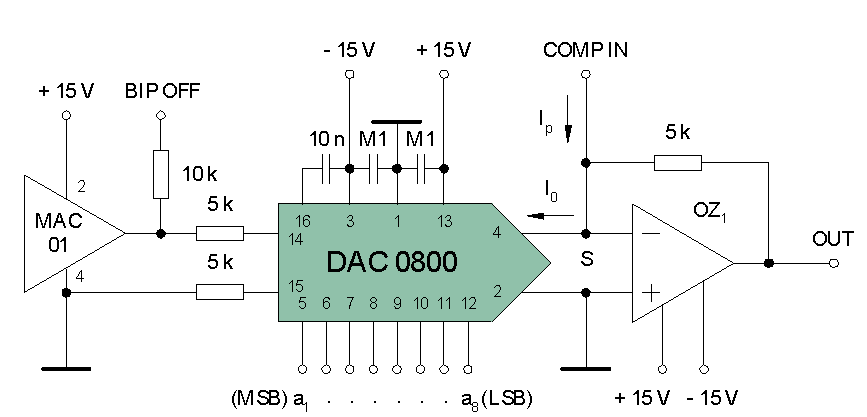
\includegraphics[width=1\linewidth]{DAC0800_sch1.pdf}
        \caption[Zapojení převodníku DAC0800]{Příklad zapojení převodníku DAC0800}
        \label{AES:fig_DAC0800_sch1}
      \end{figure}

      Příklad zapojení D/A převodníku je na obr. \ref{AES:fig_DAC0800_sch1}. Obsahuje kromě 
      vlastního D/A převodníku \texttt{DAC0800} zdroj referenčního napětí \texttt{MAC01} se 
      jmenovitým referenčním napětím +10 V a invertor se zesilovačem, pracujícím ve funkci 
      převodníku proudu na napětí pro realizaci napěťového výstupu převodníku. Funkce je 
      následující: Napětí $+10 V$ z \texttt{ MAC01} je pomocí odporu $5k\Omega$ převedeno na proud 
      $I_{REF} = 2 mA$, který je přiveden do kladného referenčního vstupu \texttt{DAC0800}, kde je 
      vynásoben nastavenou hodnotou číslicového signálu, zadanou pomocí osmi dvoupolohových 
      přepínačů. Poté se proud max $-2\cdot\left(1 - 2^{-8}\right) mA$ objeví na výstupu $I_0$ 
      a invertující zesilovač převede na odpovídající napětí. Zpětnovazební rezistor zesilovače 
      $5k\Omega$ určuje rozsah výstupního napětí 0 až 10 V (unipolární režim). Jsou-li svorky 
      \texttt{BIP OFF} a \texttt{COMP IN} propojeny, pak do sčítacího bodu \emph{S} je přiveden 
      proud $I_p = I_{REF}/2$ tj. 1 mA  ($I_p = 10 V/10 k\Omega$) opačného směru než $I_0$, který 
      způsobí trvalý posun výstupní napěťové úrovně převodníku o $-5 V$, takže rozsah převodníku 
      bude $\pm5 V$ (bipolární režim) a hodnota výstupního napětí je určena dvojkovým kódem s 
      posunutím (MSB určuje polaritu výstupního napětí).

} % tikzset
%---------------------------------------------------------------------------------------------------
\printbibliography[title={Seznam literatury}, heading=subbibliography]
\addcontentsline{toc}{section}{Seznam literatury}  
%=============== Kapitola: Kmitočtové filtry ======================================================
  % !TeX spellcheck = cs_CZ
{\tikzset{external/prefix={tikz/AES/}}
 \tikzset{external/figure name/.add={ch06_}{}}
%---------------------------------------------------------------------------------------------------
% file filter.tex
%---------------------------------------------------------------------------------------------------
%==================Kapitola: Kmitočtové filtry======================================================
\chapter{Kmitočtové filtry}
\minitoc

  \section{Základní vlastnosti kmitočtových filtrů}
    \subsection{Kmitočtové filtry a jejich použití}
      Kmitočtové filtry jsou lineární elektrické obvody, používané v mnoha oblastech elektrotechniky
      a elektroniky. Jejich hlavním úkolem je \emph{výběr} (selekce) \emph{kmitočtových složek}
      procházejícího signálu podle jejich kmitočtů. Filtry obvykle některé kmitočtové složky signálů
      \emph{propouštějí} bez útlumu (oblast se nazývá propustným pásmem), jiné kmitočtové složky
      \emph{potlačují} (pásmo potlačení, útlumu, nebo nepropustné pásmo). Tyto vlastnosti obvykle
      vyjadřujeme \emph{modulovou (amplitudovou) kmitočtovou charakteristikou} (závislost modulu
      napěťového přenosu na kmitočtu).

      Příklad použití kmitočtového filtru ukazuje názorně obr. \ref{aes:fig007}. Užitečný 
      obdélníkový signál byl znehodnocen níz\-ko\-frek\-ven\-ční rušivou harmonickou složkou 
      (pronikající např. z napájecí střídavé sítě - kmitočet sítě je nižší, než kmitočty užitečných 
      složek), signál je označen v grafu jako \(u_1(t)\). Jak je z obrázku vidět, filtr typu horní 
      propust propustil všechny kmitočtové složky s mezním kmitočtem vyšším než \(f_M\) (složky 
      obdélníkového signálu) a potlačil tak nízkofrekvenční rušivou harmonickou složku, výsledný 
      signál je v grafu označen jako \(u_2(t)\). Z obr \ref{aes:fig007} je zřejmé, že vliv 
      kmitočtových filtrů na signál je dobře patrný zvláště při znázornění procesu filtrace v 
      kmitočtové oblasti pomoci kmitočtového spektra - tedy pomoci rozkladu signálu na jeho 
      jednotlivé harmonické složky.

      Průchod signálu filtrem vede též obvykle k \emph{časovému zpožděni signálu}, což je důsledkem
      fázových posuvů (zpoždění) procházejících harmonických kmitočtových složek signálu. Ty\-to 
      vlivy obvykle vyjadřujeme \emph{fázovou kmitočtovou charakteristikou}. Jejich vliv na výstupní
      signál je též zřejmý při znázornění signálu a vlastností filtru v \emph{časové oblasti} (např.
      odezva na jednotkový skok). Fázové vlivy filtru na signál v propustném kmitočtovém pásmu se v
      časové oblasti projevují např. jako nežádoucí překmity či zvlnění průběhu signálu. V příkladu
      z obr. \ref{aes:fig007} (filtr typu horní propust) způsobil tento efekt zešikmení horních a 
      spodních hran obdélníkového signálu. Uvedené vlivy je možné vhodnou volbou filtru 
      minimalizovat. Na druhé straně ale existují případy, kdy těchto vlastností filtrů záměrné 
      využíváme, např. ve fázovacích a zpožďovacích obvodech.

      \begin{figure}[ht!]
        \centering
        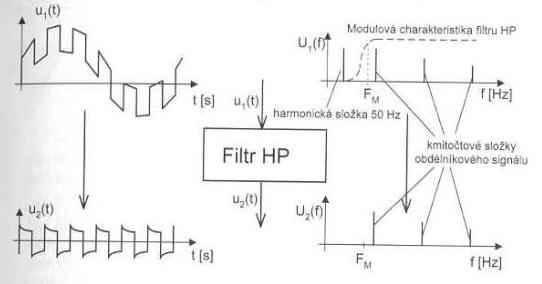
\includegraphics[width=0.9\linewidth]{aes_fig007.jpg}
        \caption{Příklad selekce kmitočtových složek signálu filtrem typu horní propust pro 
                 potlačení nízkofrekvenční rušivé složky (např. kmitočet sítě \SI{50}{\Hz)}}
        \label{aes:fig007}    
      \end{figure} 
        
      \subsubsection{Oblasti a příklady použití kmitočtových filtrů}
        Kmitočtové filtry patří mezi základní stavební bloky pro zpracování signálů. V radiotechnice
        je časté použití pásmových propustí pro výběr přijímaných signálů (vstupní obvody přijímačů,
        mezifrekvenční filtry), dolních propustí a horních propustí jako výhybek pro rozdělení
        kmitočtových pásem v anténních obvodech a předzesilovačích, pásmových zádrží pro potlačení 
        rušících signálů, dolních propustí pro různé typy demodulátorů atd. Moderní komunikační 
        systémy s rozloženým spektrem vyžadují také jako jeden z důležitých bloků přijímače filtr 
        typu pásmová propust. Obdobné je využití filtrů v telekomunikacích, při přenosu dat apod.
    
        V elektroakustice se velmi často využívají korekční filtry (nastavitelné korektory hloubek,
        výšek, pásmové korektory, korektory kmitočtových charakteristik dynamických přenosek,
        magnetofonových hlav), různé typy filtrů v systémech omezení šumu (Dolby apod ). Dolní,
        horní a pásmové propusti tvoří kmitočtové výhybky pro reproduktorové soustavy (pasivní i
        aktivní), jak ukazuje obr. \ref{aes:fig_KF_sedlacek_kmvhb}. V oblasti elektronické hudby se
        využívají i různé filtry pro zabarvení zvuku a realizaci zvláštních zvukových efektů.
      
        \begin{figure}[ht!]
          \centering
          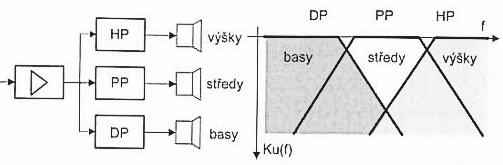
\includegraphics[width=0.9\linewidth]{KF_sedlacek_kmvhb.jpg}
          \caption[Příklad použití filtrů v kmitočtových výhybkách reproduktorových
                   soustav]{Příklad použití filtrů v kmitočtových výhybkách reproduktorových
                   soustav}
          \label{aes:fig_KF_sedlacek_kmvhb}    
        \end{figure} 
      
        Kmitočtové filtry se využívají také v oblasti \emph{měřicí techniky}. Velmi často jsou to
        filtry pro výběr měřeného kmitočtového pásma, obzvláště pak v různých typech selektivních
        měření (selektivní voltmetry, měřiče harmonického a dalších typů zkreslení, různá
        vysokofrekvenční měření). Pro akustická měření se využívá několika typů váhových filtrů pro
        měření úrovně akustického signálu (modeluje se vnímání lidského ucha). Často se využívá
        korektorů kmitočtových vlastností snímacích čidel. I přes rozvoj číslicových kmitočtových
        filtrů je výhodné u slabých a hodně zarušených signálů provést před A-D převodem analogovou
        předfiltraci pro podstatné zvýšení dynamického rozsahu systému.

        Zvláštní skupinu aplikací tvoří filtry typu dolní propust v systémech pro převod analogového
        signálu na číslicový. Pro splnění vzorkovacího teorému je zde v mnoha případech potřebné
        použit \emph{antialiasingový filtr} pro zamezení překládání rušivého spektra do užitečného
        signálu a na výstupu takového systému obdobný rekonstrukční filtr. Kmitočtové filtry se
        používají často v \emph{regulační technice}, speciální odrušovací filtry nacházejí uplatnění
        v \emph{silnoproudé elektrotechnice}. Takto bychom mohli vyjmenovat mnoho dalších aplikací.

        Lze říci, že neexistuje oblast elektrotechniky a elektroniky, kde se alespoň v omezené míře
        nevyužívají kmitočtové filtry. Základní orientace a znalost problematiky kmitočtových filtrů
        je proto potřebná prakticky pro každého tvůrčího pracovníka v elektrotechnice.
    
      \subsubsection{Způsoby realizací kmitočtových filtrů}
        Kmitočtové filtry můžeme v praxi realizovat mnoha odlišnými způsoby, které do určité míry
        určují i některé podstatné provozní vlastnosti filtru. Nejvhodnější způsob realizace je
        potřebné si pro daný účel optimálně vybrat. Tyto způsoby realizací lze rozdělit orientačně
         do tří hlavních skupin:
        \begin{itemize}
          \item Realizace z \textbf{diskrétních prvků} (odpory, kondenzátory, cívky, operační
                zesilovače apod), kde si každý uživatel může s menšími či většími problémy sestavit
                filtr přesné podle svých požadavků.
          \item Realizace v podobě \textbf{integrovaného bloku} je obvykle menší, levnější a lépe
                propracovaná, protože ji výrobce vyrábí ve velkých sériích vhodnou technologii. Na
                druhé straně si však uživatel obvykle nemůže upravit tento filtr podle svých
                speciálních požadavků a musí přesně dodržet podmínky zapojení podle výrobce.
          \item Realizace s \textbf{číslicovými filtry} spočívá v číslicovém zpracování signálu, kdy
                číslicovou interpretaci signálu matematicky upravujeme tak, aby výsledný signál měl
                po zpětném převodu shodné (či dokonce lepší) vlastnosti jako po průchodu normálním
                kmitočtovým filtrem. Matematicky tak modelujeme požadované vlastnosti filtrů a tímto
                způsobem lze dokonce realizovat i některé funkce a vlastnosti, které běžnými
                analogovými filtry nelze dosáhnout. Při realizaci jsme však omezeni na prostředí
                číslicového zpracování signálu (převodníky, počítač či signálový procesor, vhodný
                program). Značným omezením může být i maximální rychlost výpočtu počítače a
                vzorkování a tím i použitelné kmitočtové pásmo filtru.         
        \end{itemize}
        Jak je z tohoto dělení zřejmé, pro optimální výběr realizace filtru neexistuje univerzální
        návod, vždy záleží na podmínkách úlohy. Jde-li o úlohu, kdy řešíme číslicové zpracování
        signálu a máme dostatečnou výpočetní kapacitu daného prostředku, zvolíme číslicový filtr. V
        jiných případech (vysoký kmitočet signálů, slabý a zarušený signál, jde-li o výkonovou
        aplikaci apod.), použijeme analogový filtr. Při tomto řešení dáváme přednost standardnímu
        integrovanému filtru profesionální výroby (např. mezifrekvenční filtry přijímačů). Pokud
        však našim požadavkům plně nevyhovuje, musíme navrhnout a vyrobit filtr požadovaných
        vlastností z dostupných diskrétních součástek. Složitost a rozmanitost vlastností
        jednotlivých realizací filtrů ukazuje i jejich následující podrobnější přehled, který
        rozděluje jednotlivé typy filtrů podle použitých stavebních prvků:
        \begin{itemize}
          \item \textbf{Filtry RC} vynikají svou jednoduchostí, dostupností a nízkou cenou výchozích
                součástek, rezistorů a kondenzátorů. Plné však u nich platí:za málo penéz - málo
                muziky. Praktické využití mají jen jednoduché filtry prvního řádu a druhého řádu s
                nízkým činitelem jakosti (\(Q < \num{0.5}\)). Filtry RC vyšších řádů se v praxi
                používají výjimečně.
          \item \textbf{Filtry RLC} umožňují realizovat teoreticky libovolný typ filtru. Jejich
                omezeni vyplývá především z použití cívek. Ty jsou obzvláště pro nízké kmitočty
                (velké hodnoty L) rozměrné, drahé a ztrátové (malý činitel jakosti \(Q\)). Obecné je
                také použití filtrů RLC omezeno vlastními ztrátami cívek a kondenzátorů a také
                tolerancí a stabilitou jejich hodnot pro propusti a zádrže s velmi malou relativní
                šířkou pásma. Obvykle jsou používány v kmitočtovém rozsahu od \SI{100}{\kilo\hertz}
                do \SI{300}{\mega\hertz}, pro nižší kmitočty jen výjimečné. Pro kmitočty nad
                hranicí asi \SI{300}{\mega\hertz} se výrazné projevují parazitní vlastnosti prvků a
                je lépe využít realizaci s rozprostřenými parametry - viz následující bod.
          \item \textbf{Mikrovlnné filtry} jsou realizací RLC filtrů v oblasti mikrovln (\(f
                \SI{>>300}{\mega\hertz}\)), kde již nelze použít prvky se soustředěnými parametry
                (R, L, C), ale používá se odpovídající realizace s rozloženými parametry jako jsou
                vlnovody, mikropásková vedení, koaxiální vedeni apod.
          \item \textbf{Filtry ARC} (známé také jako \emph{aktivní filtry RC}) v principu nahrazují
                filtry RLC Místo cívek používají rezistory. kondenzátory a aktivní prvky, nejčastéji
                operační zesilovače. Mají obdobné vlastnosti jako filtry RLC. ale vzhledem k
                vlastnostem aktivních prvků se jejich použití omezuje nejčastéji na kmitočtové pásmo
                přibližné \SI{0.1}{\hertz} až \SI{100}{\kilo\hertz}. Současný pokrok v technologii
                aktivních prvků však umožňuje využití těchto filtrů na stále vyšších kmitočtech
                (dnes již řádové jednotky až desítky \si{\mega\hertz}), i když toto použití je zatím
                málo rozšířené. Kmitočtově jsou tedy vhodným doplňkem k filtrům RLC. Oproti nim mají
                výhodu i v snazší nastavitelnosti a laditelnosti změnou hodnot odporů. Jejich
                nevýhodou je na druhé straně potřeba napájení aktivních prvků. Objevují se i jejich
                specifické modifikace využívající parazitních vlastností aktivních prvků (R nebo C)
                jako stavebních prvků - filtry AC. AR apod.
          \item \textbf{Filtry ASC}, známé též jako \emph{filtry se spínanými kapacitory} jsou
                speciální modifikaci filtru ARC. které místo odporů používají přepínané
                kondenzátory. Jejich hlavní výhodou je možnost poměrně snadné monolitické integrace
                v porovnání s filtry ARC. Některé typy můžeme zakoupit jako integrované obvody.
                Jejich mezní kmitočet je určen spínacím kmitočtem a jsou tedy snadno přeladitelné.
                Lze je řadit již do skupiny integrovaných filtrů, nicméně jsou zde možnosti
                určitého přizpůsobení požadavkům, a to jednak přeladěním, jednak také dostupnosti
                integrovaných nastavitelných bloků 2. řádu. Na druhé straně je však tento typ
                realizace kmitočtově ještě více omezen než filtry ARC a má navíc problémy s vyšším
                driftem, s určitým průnikem spínacího signálu do užitečného signálu a
                „schodovitostí“ výsledného signálu, způsobenou spínáním. Spínací kmitočet bývá
                \(\num{50}\times\) až \(\num{100}\times\) vyšší než mezní kmitočet filtru, což do
                určité míry minimalizuje spínáním vzniklý projev diskretizace signálu v časové
                oblasti a možný aliasingový efekt (překládání spektra rušivého signálu do spektra
                užitečného signálu).
          \item \textbf{Elektromechanické filtry} jsou historicky nejstarší „integrované“ filtry.
                Vycházejí z principu převodu elektrického signálu na mechanický, využitím nékteré
                formy mechanické rezonance a zpětného převodu výsledného mechanického signálu na
                elektrický. Chovají se tedy vesměs jako pásmové propusti. Podle typu mechanického
                rezonátoru je lze dělit na různé skupiny. Dříve byly používány např. magnetostrikční
                filtry a dnes jsou používané nejčastěji \emph{piezokeramické filtry} (např.
                mezifrekvenčni filtry \SI{455}{\kilo\hertz} a \SI{10.7}{\mega\hertz}).
                Zvláštním typem je \emph{krystalový filtr}, který odpovídá v podstatě složenému
                rezonančnímu obvodu s vysokým činitelem jakosti (řádové \num{10000}) a vysokou
                stabilitou rezonančního kmitočtu. Nejčastěji se využívá ve stabilních oscilátorech.
                Vzhledem k vysokému a nenastavitelnému činiteli jakosti a nenastavitelnému
                rezonančnímu kmitočtu se krystaly jako filtry používají velmi omezené. Zapojením
                většího počtu krystalů s velmi přesným výběrem lze realizovat úzký pásmový filtr pro
                speciální aplikace jako např. úzkopásmové mezifrekvenčni filtry s vysokým
                rezonančním kmitočtem.
          \item \textbf{Filtry s PAV} (s \emph{povrchovou akustickou vlnou}, anglická zkratka SAW)
                jsou poměrné novým typem integrovaných filtrů, založených na principu vyzařování,
                šíření a fázového, kmitočtově závislého skládání povrchových akustických vln.
                Realizují se tak, že se nanese na nosnou keramickou destičku soustava vysílacích a
                přijímacích piezoelektrických zářičů, jejichž tvar a funkci lze přirovnat k dvěma
                Yagiho anténám. Obdobně jako u antén je rozměry a polohou zářičů tvarována přenosová
                kmitočtová charakteristika filtru. V porovnání s elektromechanickými filtry mohou
                realizovat podstatně širokopásmovéjší obvody. Proto se s výhodou používají, např.
                jako obrazové mezifrekvenčni filtry v televizorech a v mnoha dalších aplikacích pro
                vysoké kmitočty. Na druhou stranu je jejich použití částečné omezeno vyšším
                průchozím útlumem.
          \item \textbf{Filtry CCD} (\emph{charge coupled devices - nábojové vázané obvody}) jsou
                dalším speciálním typem aplikace s časové diskrétním charakterem (např. jako filtry
                ASC). Využívá se u nich technologie známá např. z CCD televizních kamer a princip
                spočívá v postupném posuvu a fázově závislém sčítání jednotlivých „nábojových
                vzorků“.
          \item \textbf{Číslicové filtry} jsou oproti předchozím filtrům odlišnou („softwarovou“)
                realizaci funkce filtrů, jejich princip byl popsán v předchozím odstavci.
        \end{itemize}
        Uvedený přehled potvrzuje značnou různorodost konečných realizací filtrů. Z přehledu
        vlastností jednotlivých typů kmitočtových filtrů je zřejmá i obtížnost úlohy konstruktéra
        při výběru optimálního způsobu realizace. Pro rychlejší orientaci o použitelnosti
        uvedených filtrů z hlediska kmitočtového pásma je možné využít tab.
        \ref{aes:fig_KF_sedlacek_kmtab}. Meze použití jednotlivých způsobů realizací je nutno chápat
        jen jako orientační, protože závisí nejen na současném stavu technologie, ale i na mnoha
        různých parametrech a požadavcích kladených na filtry.

        \begin{figure}[ht!]
          \centering
          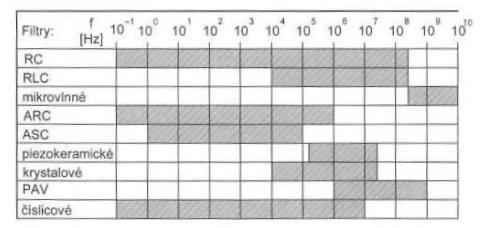
\includegraphics[width=0.9\linewidth]{KF_sedlacek_kmtab.jpg}
          \caption[Orientační znázornění kmitočtových pásem použitelnosti jednotlivých typů
                   realizaci filtrů]{Orientační znázornění kmitočtových pásem použitelnosti
                   jednotlivých typů realizaci filtrů}
          \label{aes:fig_KF_sedlacek_kmtab}    
        \end{figure} 
  
  \section{Popis přenosových vlastností filtrů, jejich charakteristiky}
    \subsection{Průchod signálu kmitočtovým filtrem a přenosové kmitočtové charakteristiky filtrů}
      Základní zapojeni filtru připojeného ke zdroji harmonického signálu je uvedeno na obr.
      \ref{aes:fig_KF_sedlacek_dvjbrn}. Procházi-li přes kmitočtový filtr harmonický signál s
      amplitudou \(U_1\), kmitočtem \(f_1\) a fázi \(\varphi_1\), získáme na výstupu filtru opět
      harmonický signál se stejným kmitočtem, ale jinou velikostí amplitudy a fáze (\(U_2\),
      \(\varphi_2\)).
  
      \begin{figure}[ht!]
        \centering
        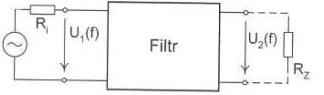
\includegraphics[width=0.8\linewidth]{KF_sedlacek_dvjbrn.jpg}
        \caption[Filtr jako dvojbran]{Filtr jako dvojbran}
        \label{aes:fig_KF_sedlacek_dvjbrn}    
      \end{figure}
      
      \textbf{Přenos napětí} \(\mathbb{K_U}\) harmonického signálu filtrem lze pro daný kmitočet
      \(f\) vyjádřit komplexním výrazem
      \begin{equation}\label{aes:eq_KF_ku}
        \mathbb{K_U} = K_U\cdot e^{j\varphi} = \frac{U_2e^{j\varphi_2}}{U_1e^{j\varphi_1}},
      \end{equation}
      který můžeme rozdělit na \emph{reálnou} a \emph{imaginární} část. Častěji ale používáme
      vyjádření přenosu pomocí \emph{modulu} a \emph{argumentu}
      \begin{equation}\label{aes:eq_KF_moarg}
        K_U = \frac{U_2}{U_1}, \qquad \varphi = \varphi_2 - \varphi_1, 
      \end{equation}
      kde modul \(K_U\) je poměr amplitud výstupního a vstupního signálu a argument \(\varphi\) je
      výsledný fázový posuv (časový rozdíl vztažený na periodu) mezi výstupním a vstupním signálem
      jako rozdíl fázi výstupního signálu \(\varphi_2\) a vstupního signálu \(\varphi_1\). Modul
      přenosu \(K_U\) je bezrozměrné číslo a často se udává v logaritmické míře, kdy platí \(K_U
      [\si{\decibel}] = 20 \log{K_U}\). Toto běžné používané vyjádření umožňuje grafické znázornění
      velkého rozsahu hodnot.
  
  \section{Přenosové vlastnosti a charakteristiky základních typů filtrů}
    \subsection{Filtry s přenosovou funkcí 1. řádu}
    \subsection{Filtry s přenosovou funkcí 2. řádu}
    \subsection{Přenosové funkce vyšších řádů}
    \subsection{Citlivost a tolerance přenosových vlastností filtrů} 
  \section{Návrh filtrů RC a RLC 1. a 2. řádu}
    \subsection{Návrh filtrů RC}
    \subsection{Návrh filtrů RLC 2. řádu}
    \subsection{Návrh fázovacích článků RLC 1. a 2. řádu}     
  \section{Filtry RLC vyšších řádů}
    
  \section{Filtry ARC 2. řádu}
    \subsection{Základní principy funkce filtrů ARC}
      Při realizaci filtrů RLC pro nízké kmitočty jsou největší problémy s kvalitou, rozměry a
      cenou cívek. Proto se pro nízké kmitočty s výhodou nahrazují \textbf{aktivními filtry RC}
      (filtry ARC). Jejich základní princip spočívá v "náhradě" cívky pomocí zapojení
      \emph{aktivního prvku} (operační zesilovač, tranzistor) se dvěma rezistory a kapacitory.
      Nahradit cívku můžeme v zásadě dvěma základními způsoby. První spočívá v použití obvodu,
      který přímo nahrazuje cívku jako dvojpól a vykazuje mezi určitými svorkami příslušnou
      indukčnost. Druhý princip, jak bude ukázáno dále, nahrazuje cívku nepřímo, pomoci
      transformace výchozího LRC obvodu na ekvivalentně se chovající strukturu RCD, která indukční
      prvek neobsahuje, ale na druhou stranu potřebuje \emph{syntetický prvek D} - dvojný kapacitor
      (kmitočtově závislý negativní rezistor).

    \subsection{Obvody s náhradou cívky}
      Aktivní filtry ARC, které vycházejí z filtru RLC a využívají k tomu přímou či nepřímou
      náhradu cívek, mají velké množství různých variant zapojeni. Objasnění jejich funkce
      představuje i řadu různých pohledů na činnost filtru. V oblasti návrhu ARC filtru převažují
      dva hlavni přístupy. Velmi názorný je takový přístup, který vytváří obvody, vykazující na
      vstupních svorkách induktivní impedanci. Ty lze využít jako přímou náhradu indukčnosti ve
      filtru RLC. Zřejmě nejčastější je ale takový pohled, kdy vytváříme celý obvod ARC s
      přenosovou funkci 2. řádu jako ekvivalenci obvodu LRC 2. řádu, přičemž přímá náhrada cívky v
      obvodu nemusí být na první pohled zřejmá.

    \subsection{Stavební prvky filtrů ARC a základní vlivy jejich reálných vlastností}
      Stavebními prvky filtrů ARC jsou rezistory, kapacitory a aktivní prvky, jak již bylo
      naznačeno v předešlém textu. I pro nejjednodušší posouzení funkce, klasifikaci a výběr
      optimálního zapojeni filtrů ARC je potřeba rozumět alespoň základním vlivům reálných
      vlastnosti těchto stavebních prvků na výsledné parametry ARC obvodu.

      \subsection{Vliv reálných odporů a kondenzátorů}
        ($C_1$, i $C_2$) vytvářejí se zbytkem obvodu rezonanční obvod RLC, lze vliv jejich ztrát
        modelovat sériovým či paralelním spojením ideálního kapacitoru s rezistorem. Tento vliv lze
        posuzovat v principu shodně jako u filtrů RLC. Při ideálních vlastnostech zbývající části
        obvodu určuje hodnotu činitele jakosti celkového obvodu činitel jakosti reálného
        kondenzátoru $Q_c = \frac{1}{tg\delta}$. Jeho hodnota musí být proto podstatně vyšší než
        výsledná funkční hodnota činitele jakosti celého obvodu (alespoň \(\num{10}\times\)). Při
        nižších hodnotách je třeba tento vliv brát v úvahu a pokud je to možné, kompenzujeme jej
        snížením vnějšího zatlumení tak, aby výsledné \emph{Q} odpovídalo požadovanému. Je potřebné
        si uvědomit, že ztráty kondenzátorů může obdobně zvýšit i sériové či paralelní spojení
        kondenzátorů s parazitními odpory, jako je např. vnitřní odpor zdroje, parazitní vstupní a
        výstupní odpor aktivních prvků apod.
        
  \section{Filtry ARC vyšších řádů}
  \section{Filtry se spínanými kapacitory}
  \section{Zváštní typy a aplikace kmitočtových filtrů}      

} % tikzset
%---------------------------------------------------------------------------------------------------
\printbibliography[title={Seznam literatury}, heading=subbibliography]
\addcontentsline{toc}{section}{Seznam literatury}
%=============== Kapitola: Autonomní zdroje elektrické energie ====================================
  % !TeX spellcheck = cs_CZ
{\tikzset{external/prefix={tikz/AES/}}
 \tikzset{external/figure name/.add={ch07_}{}}
%---------------------------------------------------------------------------------------------------
% file batt.tex
%---------------------------------------------------------------------------------------------------
%========= Kapitola: Autonomní zdroje elektrické energie ===========================================
\chapter{Autonomní zdroje elektrické energie}
\minitoc
  Většina přenosných elektronických zařízení potřebují ke své činnosti zdroj elektrické energie a 
  to nejčastěji ve formě stejnosměrného DC výkonu. Každý napájecí zdroj lze podle Theveninovy věty 
  nahradit sériovým spojením ideálního zdroje napětí a jeho vnitřního odporu. Vlastní zátěž lze 
  často nahradit lineárním rezistorem. Skutečná povaha napájecího zdroje bývá často složitější, 
  mívají charakter setrvačný, nelineární,pa\-ra\-me\-tri\-cký apod. Dokonce se někdy k malé radosti 
  setkáme 
  i se zdroji, které mají vnitřní odpor záporný. Definiční vztahy pro vnitřní a zatěžovací odpor 
  napájecího zdroje jsou následující
  \begin{itemize}
    \item \textbf{Vnitřní (výstupní) odpor zdroje}:
          \begin{equation}\label{aes:eq010}
            R_i = \frac{U_{2a}-U_{2b}}{I_{2a} - I{2b}} = -\der{U_2}{I_2}
          \end{equation}
    \item \textbf{Zatěžovací odpor}:
          \begin{equation}\label{aes:eq011}
            R_z = \frac{U_2}{I_2}
          \end{equation}
  \end{itemize}
  Přitom záporné znaménko ve vztahu (\ref{aes:eq010}) vyjadřuje skutečnost, že v obvyklém případě 
  zvýšení výstupního odebíraného proudu \(I_2\) způsobí snížení výstupního napětí \(U_2\). Pomocí 
  těchto dvou jednoduchých vztahů lze také rozlišit \textbf{zdroj napětí} \(– R_i \ll R_L\) od 
  zdroje proudu \(- R_i\gg R_L\). U elektronických napájecích zdrojů je běžné, že do určitého a 
  často nastavitelného zatěžovacího proudu se obvod chová jako zdroj napětí, po jeho překročení 
  jako zdroj proudu. Tomuto opatření říkáme \emph{nadproudová ochrana, omezení proudu, elektronická 
  pojistka}. Situace je na obr. 1-1.
  
  \section{Bateriové způsoby napájení}
    Bateriové napájení je výhodné svou nezávislostí na napájecí síti a tedy drátovém přívodu. 
    Vzhledem ke stále klesající spotřebě energie u napájených zařízení a rostoucí kvalitě 
    chemických zdrojů je tento způsob dnes velmi oblíbený.
   
    Je všeobecně známo, že bateriové (chemické) zdroje lze rozdělit na \textbf{primární} 
    (\emph{nenabíjitelné}) a \textbf{sekundární} (\textbf{a\-ku\-mu\-lá\-to\-ry}) – 
    \emph{nabíjitelné}. Rozdíly se dnes už stírají, existují např. baterie typu RAM,  které patří 
    mezi primární s možností nabíjení.
    
    \subsection{Primární (galvanické) články}
      Primární články přeměňují přímo chemickou energii v energii elektrickou a patří k velmi 
      starým zdrojům.
    \subsection{Sekundární články, akumulátory}
    \subsection{Palivové články}
    \subsection{Termoemisní generátory}
    \subsection{Termoelektrické články}
    \subsection{Sluneční (solární) , fotovoltaické články}
    
} % tikzset
%---------------------------------------------------------------------------------------------------
\printbibliography[title={Seznam literatury}, heading=subbibliography]
\addcontentsline{toc}{section}{Seznam literatury}

%=============== Kapitola: Spojitě regulované napájecí zdroje =====================================
  % !TeX spellcheck = cs_CZ
%---------------------------------------------------------------------------------------------------
% file lin_reg_power.tex
%---------------------------------------------------------------------------------------------------
%====================== Kapitola: Spojitě regulované napájecí zdroje ===============================
\setchaptertoc
\chapter{Spojitě regulované napájecí zdroje}


  \section{Metody snímání proudu v napájecích zdro\-jích}
  \section{Neřízené usměrňovače}
    \subsection{Usměrňovače s nesetrvačnou zátěží}
    \subsection{Usměrňovače se sběrným kondenzátorem (s RC zátěží)}
    \subsection{Usměrňovače s nárazovou tlumivkou (s RL zá\-tě\-ží)}
      Základní schéma zapojení je na obr. \ref{enz:fig_usm_1f_RLz}. Obsah vyšších rušivých harmonických produktů lze snížit sériově se zátěží zapojeným obvodem typu hornofrekvenční zádrž. I zde je filtrační účinek závislý na poměru zatěžovací konstanty $\tau_L=\frac{L}{R_L}$ a doby periody $T=\frac{1}{f}$ - je to činitel $K=\tau_L/T$. $(K \uparrow: \tau_L\uparrow,T\downarrow\Rightarrow L\uparrow,R_L\downarrow)$. Tyto usměrňovače jsou tedy výhodné pro zátěže typu "malé napětí x velký proud". I tady lze elegantně podpořit velkou hodnotu koeficientu $K$ tím, že obvod budeme napájet signálem o vysokém kmitočtu. Zatím co v případě RC zátěže byl kondenzátor pamětí napětí, tady použitá tlumivka je naopak pamětí proudu. Z toho důvodu je např. jednocestné zapojení s nárazovou tlumivkou fyzikálně nevhodné, protože mohou nastat jen dva krajní (a oba špatné) případy.
      \begin{figure}[ht!]
        \centering
        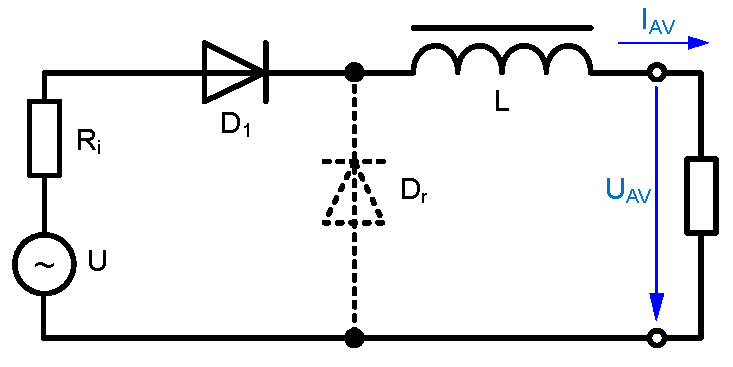
\includegraphics[width=0.6\linewidth]{patocka_jednocestny_1f_usm_LRzatez.pdf}
        \caption{Jednocestný jednofázový usměrňovač RL zátěží.}
        \label{enz:fig_usm_1f_RLz}
      \end{figure}

      \begin{itemize}[noitemsep]
        \item Bude-li indukčnost veliká (v limitě nekonečná), pak podle Lenzova pravidla udrží  
              proud v obvodu (je celý v sérii) na stálé hodnotě i co do směru, dioda se nemůže 
              vůbec uzavřít a obvod nemůže usměrňovat - nebude mít střídavou složku.
        \item Naopak při malé hodnotě (proti jakési kritické) dioda zavře, obvod se přeruší a  
              energie magnetického pole cívky (je vázána existencí proudu) se nemůže uplatnit v 
              překlenutí mezer dodávky energie na výstup. Při dalším otevření diody můžou navíc 
              nastat přechodné děje.
      \end{itemize}

      Existuje však velice jednoduchá a plně funkční úprava a tou je doplnění jednocestného usměrňovače tzv. \textbf{rekuperační (nulovou) diodou} -
      $D_R$ (kreslena čárkovaně viz obr. \ref{enz:fig_usm_1f_RLz}). Při uzavření hlavní diody $D_1$ se tlumivka snaží držet proud obvodem ve stejné
      velikosti a ve stejném směru a tento proud otevře rekuperační diodu $D_R$.

      Mezi filtrací se sběrným kondenzátorem (RC zátěží) a s nárazovou tlumivkou (RL zátěží) je 
      ještě zajímavý rozdíl: filtrace paralelním kondenzátorem pracuje s hyperbolicky se měnící 
      impedancí $X_C=\frac{1}{\omega C}$ a potlačení vysokých čísel harmonických je čím dál tím 
      menší.  Obvod se sériovou tlumivkou pracuje s impedancí $X_L=\omega L$ a potlačující efekt 
      lineárně roste. \emph{Zvlnění na RC zátěži má proto obvykle dosti značný obsah vysokých 
      harmonických a je pilovitého průběhu. Zvlnění na RL zátěži je za stejných podmínek $K$ 
      harmonicky čistší a má charakter sinusovky.}


      % --------example: Usměrňovač --------------------------
      % \label{AES:exam001}
      % !TeX spellcheck = cs_CZ
\begin{example}\label{AES:exam001}
  Proveďte simulaci vyznačených obvodových veličin obvodu na obrá\-zku \ref{AES:fig_exam001_1} se 
  zadanými hodnotami prvků v programu  PSpice\footnote{Simulace je provedena v programu 
  \texttt{OrCAD PSpice} ver. 16.3}.

   {\centering
    \captionsetup{type=figure} 
    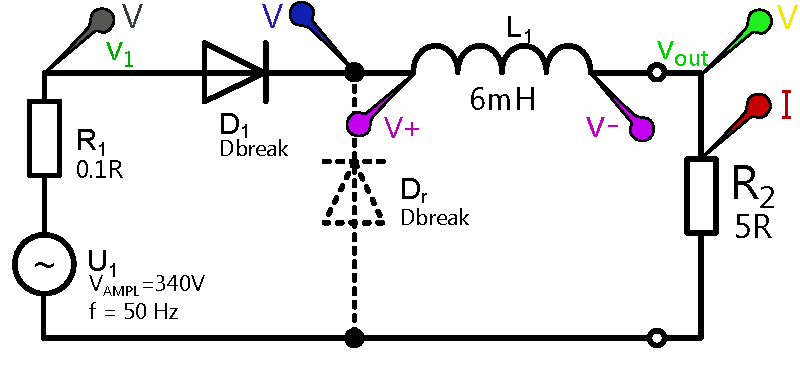
\includegraphics[width=0.8\linewidth]{patocka_jednocestny_1f_usm_PSpice.pdf}
    \captionof{figure}{Neřízený Jednofázový usměrňovač s nulovou diodu. Simulované veličiny jsou 
               vyznačeny barevnými markery.}
    \label{AES:fig_exam001_1}
    \par}

   {\centering
    \captionsetup{type=figure} 
    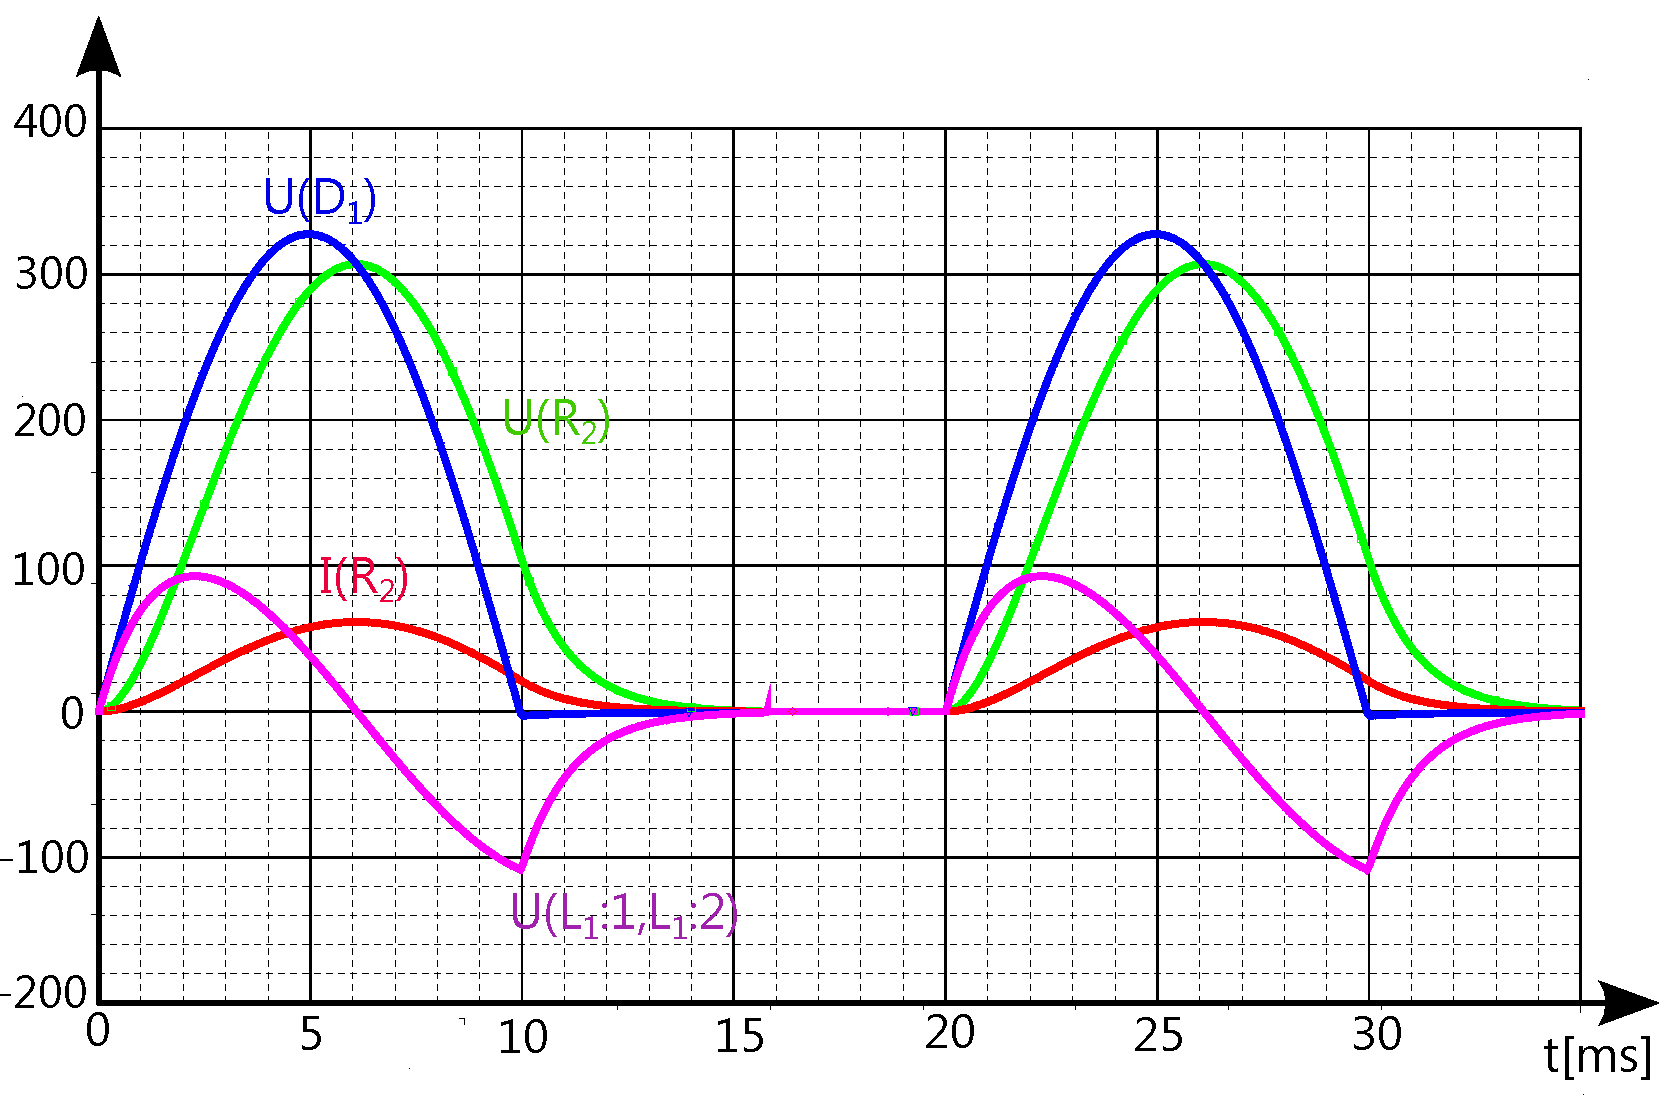
\includegraphics[width=0.9\linewidth]{PSPice_SIM002_usm1f_RL_6mH_5R.pdf}
    \captionof{figure}{Průběhy vyznačených veličin jednofázového neřízeného usměrňovače s RL zátěží 
              (6mH, 5$\Omega$) a nulovou diodou [ENZ/SIM002]}
    \label{AES:fig_exam001_2}
    \par}
\end{example}  
      %-------------------------------------------------------

  \section{Stabilizátory stejnosměrného napětí}
    Stabilizátory napětí na svém výstupu konstantní napětí v pokud možno co nejširším rozsahu 
    odebíraného výstupního proudu a dodávaného vstupního napětí \cite[s.~95]{Zahlava2001}
    \begin{itemize}
      \item nelineární (parametrické) stabilizátory napětí,
      \item lineární spojité stabilizátory napětí
    \end{itemize}

    \subsection{Nelineární (parametrické) stabilizátory}
      Využívají vlastností VA charakteristik některých jako je otevřený PN přechod, Zenerovy diody, termistory a jiné. Pro tyto účely potřebujeme tzv. prvky triodového typu u kterých platí, že \emph{dynamický vnitřní odpor je podstatně nižší jak statický}. Tedy $R_{dyn} < R_{stat}$. Pro naše účely jsou nejčastěji používané \emph{Zenerovy diody} a dvojpólové integrované \emph{napěťové referenční obvody}. Zenerovy diody jsou vyráběny jako malovýkonové ( anodová ztráta do 1W) a výkonové (obvykle 10W a více). Pro referenční účely jsou často doplněny dalšími pomocnými kompenzačními prvky. Vlastní princip nelineární\-ho spojitého stabilizátoru ( podivný název „parametrický“ nebudeme použí\-vat) je velice prostý: obvod dle obr. \ref{enz:fig_sch_ZD_stab} tvoří dělič s horním odporem lineárním a dolním (je paralelně k zátěži) tvořeným popsaným nelineárním odporem triodového typu. Za těchto okolností má tento obvod pochopitelně přenos dynamický podstatně menší jak statický a tedy je to stabilizátor napětí.

      \begin{figure}[ht!]
         \centering
         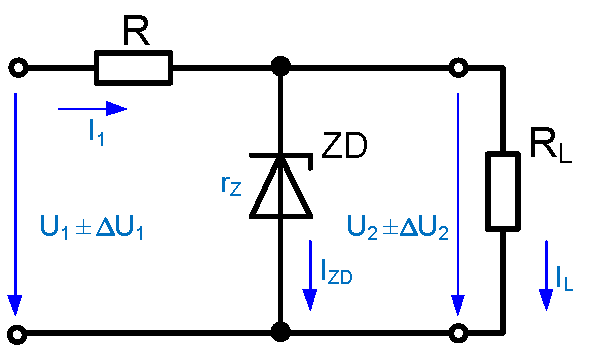
\includegraphics[width=0.6\linewidth]{patocka_stabilizator_ZD_sch.pdf}
         \caption{Nelineární spojitý stabilizátor napětí}
         \label{enz:fig_sch_ZD_stab}
       \end{figure}

      \begin{figure}[ht!]
         \centering
         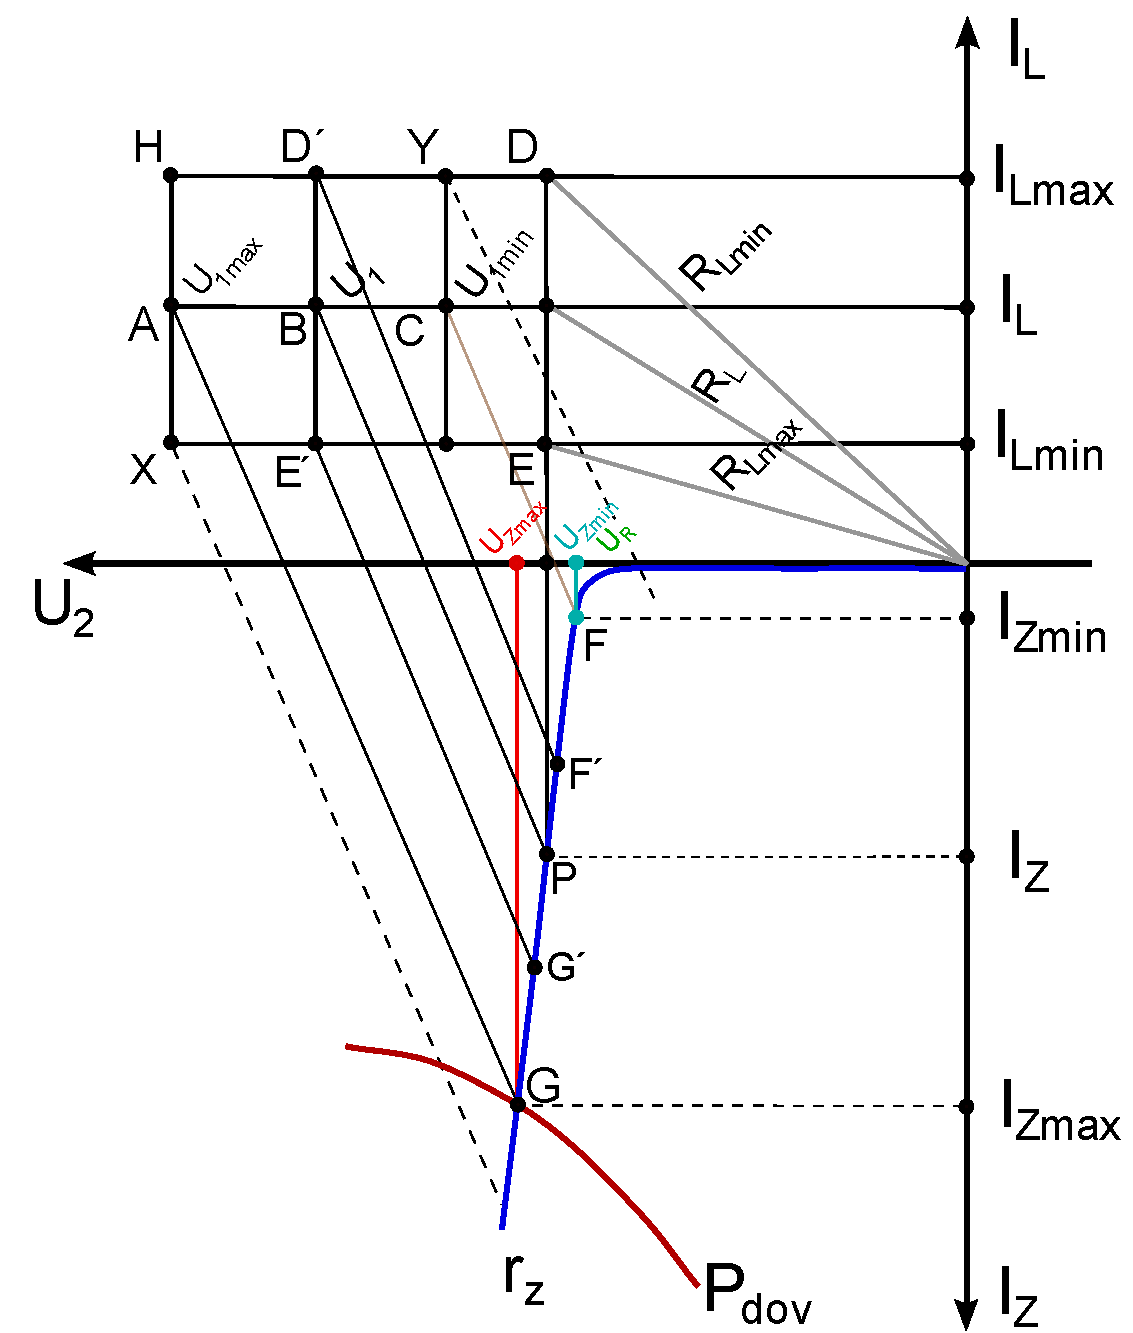
\includegraphics[width=0.8\linewidth]{patocka_stabilizator_ZD_VA.pdf}
         \caption{Grafické řešení nelineárního stabilizátoru}
         \label{enz:fig_graf_res_ZD_stab}
       \end{figure}

       Řešení je výhodné v grafické podobě - obr. \ref{enz:fig_graf_res_ZD_stab}. Ve třetím 
       kvadrantu je nakreslena VA charakteristika\footnote{Je typická určitým Zenerovým napětím 
       $U_z$, sklonem pracovní části VA charakteristiky (dynamickým vnitřním odporem  $r_z$) a 
       dovolenou anodovou ztrátou $P_{dov}$. Tato ztráta závisí na způsobu chlazení.} Bod 
       \texttt{B} odpovídá zvolenému vstupnímu napětí $U_1$ a výstupnímu proudu $I_2$ a tedy i 
       velikosti odporu $R_L$. Úloha může být nyní dána např. kolísáním vstupního napětí od 
       $U_{1_{max}}$ do $U_{1_{min}}$ (body \texttt{A} a \texttt{C}), nebo kolísáním zátěže nebo 
       proudu $I_2$ ( body \texttt{E'}a \texttt{D'}). Při současném působení změn vznikne obrazec 
       (přibližně obdélník) \texttt{X}, \texttt{E}, \texttt{D}, \texttt{H}, což je geometrické 
       místo možných stavů obvodů. Na vlastní VA charakteristice prvku pro volený "předřadný" odpor 
       \emph{R} vzniknou body \texttt{G}, \texttt{P} a \texttt{F} a to je grafické řešení. Vidíme, 
       kdy hrozí "zhasnutí" nebo přetíženi Zenerovy diody. Projekcí bodu \texttt{G}, \texttt{P} a 
       \texttt{F} na vodorovnou osu zjistíme okamžité hodnoty výstupního napětí stabilizátoru $U_2$ 
       a jeho kolísání $\Delta U_2$. Lze snadno odečíst zvládnutelné kolísání vstupního napětí či 
       velikosti zátěže atd. Z obrázku je také vidět, že zlepšení stabilizačního účinku obvodu lze 
       dosáhnout zvětšením vstupního napětí (větší odpor \emph{R}) nebo výběrem diody s menším 
       dynamickým odporem $r_z$ . Velice vtipná možnost zlepšení přenosových vlastností 
       stabilizátoru je při náhradě lineárního odporu \emph{R} nelineárním prvkem s pentodovým 
       charakterem VA charakteristiky. Může to být třeba bipolární nebo lépe unipolární tranzistor. 
       Pak vlastně Zenerovu diodu napájíme zdrojem konstantního proudu a to je hojně využívané v 
       integrovaných stabilizátorech.

       Z obr. \ref{enz:fig_sch_ZD_stab} lze snadno odvodit činitel napěťové stabilizace
       \begin{equation}\label{enz:eq_Su_ZD}
         S_u = \frac{\Delta u_{vst}}{\Delta u_{v\acute{y}st}} = \frac{R+r_z\parallel R_L}{r_z\parallel R_L} \cong \frac{R+r_z}{r_z}, \mathrm{kde} r_z\ll R_L
       \end{equation}

      % --------example: Stabilizátor ------------------------
      % \label{AES:exam002}
      % !TeX spellcheck = cs_CZ
\begin{example}\label{AES:exam002} Určete vliv nenulového dynamického odporu Zenerovy diody na 
  zvlnění výstupního napětí je-li zadáno: \(U_S = \SI{14}{\volt}, u_{ripple} = \SI{100}{\mV},
  U_Z = \SI{8}{\volt}, r_Z = \SI{10}{\ohm}, R_S = \SI{50}{\ohm}, R_L = \SI{150}{\ohm}\).
  \vspace{1em}
  
  {\centering
   \begin{tabular}{cc}
     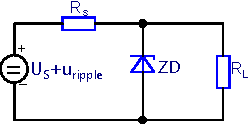
\includegraphics[width=0.4\linewidth]{stabilizator_ZD_ripple_effect.pdf}  &
     \includegraphics[width=0.5\linewidth]{stabilizator_ZD_ripple_graph.pdf}
   \end{tabular}
   \captionsetup{type=figure} 
   \captionof{figure}{K příkladu nenulového dynamického odporu Zenerovy diody na přenos zvlnění ze 
              vstupního napětí na výstupní napětí}
   \label{enz:fig_ZD_ripple}
 \par}
  \vspace{1em}
  \textbf{Řešení}:\newline Abychom stanovili velikost výstupního napětí, amplitudu zvlnění napětí 
  na zátěži a mohli také určit vliv velikosti dynamického odporu $r_z$, vyjděme z náhradního 
  lineárního obvodu na obrázku \ref{enz:fig_ZD_NLO}.
  \begin{enumerate}[noitemsep]
    \item Stejnosměrný ekvivalentní obvod:
      \begin{align}\label{enz:eq_ZD_DC_UL}
         U_L &= U_S\frac{R_L\parallel r_z}{R_S + R_L\parallel r_z}   \nonumber \\
              + U_z\frac{R_S\parallel R_L}{r_z + R_S\parallel R_L}
             &= 2.21 + 6.32 = \SI{8.53}{\volt}
      \end{align}
    \item Střídavý ekvivalentní obvod:
      \begin{equation}\label{enz:eq_ZD_AC_UL}
        u_L = v_{ripple}\frac{r_z\parallel R_L}{R_S + r_z\parallel R_L} = \SI{16}{\mV}
      \end{equation}
      Tedy jedna šestina zvlnění vstupního napětí se přenese na výstupní svorky stabilizátoru.
  \end{enumerate}

  {\centering
   \begin{tabular}{cc}
     \includegraphics[width=0.4\linewidth]{stabilizator_ZD_DC_equival.pdf}
     \includegraphics[width=0.4\linewidth]{stabilizator_ZD_AC_equival.pdf}
   \end{tabular}
   \captionsetup{type=figure} 
   \captionof{figure}{Stabilizátor se ZD lze pro výpočet jeho ss chování v okolí pracovního bodu  
            linearizovat pomocí NLO}
   \label{enz:fig_ZD_NLO}
  \par}
  Schopnost stabilizace je horší, čím větší má Zenerova dioda dynamický odpor $r_z$. Proto 
  musí být $r_z$ výrazně nižší, než hodnoty rezistorů $R_S$ a $R_L$ (viz rov. 
  \ref{enz:eq_ZD_AC_UL}).
\end{example}  
      %-------------------------------------------------------

    \subsection{Lineární spojité stabilizátory}
    
  \section{Násobiče napětí}
  \section{Ochranné a signalizační obvody zdrojů}
    \subsection{Pojistky}
       \subsubsection{Signalizace přerušené pojistky}
         Rozsvícením svítivé diody $D_1$, je uživatel upozorněn na přerušenou tavnou pojistku 
         $PO_1$ v zařízení napájeném malým napětím. Je-li pojistka v pořádku, je při zapnutém 
         vypínači $S_1$ na svítivé diodě napětí tvořené úbytky na pojistce a otevřené diodě $D_2$, 
         jenž nestačí pro její rozsvícení. Jakmile se však pojistka přeruší, dioda $D_1$ se 
         rozsvítí. Průchodu proudu spotřebičem přes $D_2$ při sepnutém vypínači $S_1$ brání její 
         polarizace.

         \begin{figure}[ht!]
           \centering
           \includegraphics[width=0.4\linewidth]{sig_cir_fuse_failure.pdf}
           \caption{Obvod signalizující přerušení pojistky v nízkonapěťovém obvodu.}
           \label{enz:fig_fuse_failure}
         \end{figure}

%---------------------------------------------------------------------------------------------------

%=============== Kapitola: Základy spínaných napájecích zdrojů ====================================
  % !TeX spellcheck = cs_CZ
%---------------------------------------------------------------------------------------------------
% file SMPS.tex
%---------------------------------------------------------------------------------------------------
%========= Kapitola: Impulzně regulované napájecí zdroje ===========================================
\setchaptertoc
\chapter{Impulzně regulované napájecí zdroje}

  \section{Úvod}\label{aes:sec010}
    Spínané napájecí zdroje plní funkci stejnou jako zdroje se spojitou regulací. Vý\-ko\-no\-vý
    člen spínacích zdrojů je však zatěžován impulzně, tj. střídavě spínán a rozepínán. Lze tedy
    využít výhody impulzního režimu, tj. odebírat impulzní výkon podstatně větší, než je trvalý
    výkon při lineárním režimu regulátoru s týmž výkonovým členem. Spínací zdroje mají obecně větší
    účinnost než zdroje se spojitou regulací. Jsou výhodné zvláště tam, kde je velký rozdíl napětí
    na vstupu a výstupu regulátoru a kde jsou požadované malé rozměry. Impulzní regulace zajistí
    stabilizované výstupní napětí i pro velké změny vstupního napětí; účinnost zdroje se při tom
    téměř nemění. I přes větší obvodovou složitost jsou ekonomicky výhodnější, neboť jejich použití
    vede k podstatné energetické úspoře.
  
    Impulzně regulované zdroje však mají v porovnání se zdroji s lineární regulací i některé
    nevýhodné vlastnosti, například pomalejší reakci výstupního napětí na rychlé změny zatěžovacího
    výstupního proudu. Při požadavku malého zvlnění výstupního napětí se nesmí zanedbat vliv
    impulzního charakteru těchto zdrojů. Impulzně regulované zdroje jsou také zdrojem rušivých
    signálů, které jsou generovány spínacími prvky \cite[s.~112]{Hammembauer}.
       
  \section{Impulzní regulace ve výkonové elektronice}\label{aes:sec005}
    Základním principem a současně odlišností impulzní regulace od regulace klasické je v její
    \emph{nespojitosti}. To znamená, že nehledě na detailní realizaci, je výstupní napětí 
    stabilizováno zásahy regulačního členu pouze v určitých, časově omezených intervalech. Podstata 
    regulačního členu (regulátoru) tedy spočívá v řízení vzájemných časových relací aktivního a 
    pasivního intervalu pracovního cyklu v závislosti na velikosti zesílené regulační odchylky.
    
    Akční člen je tedy řízen dvouhodnotovým signálem, mající význam \emph{zapnutí} nebo 
    \emph{vypnutí} výkonové součástky. Následující příklad demonstruje, jak lze tento signál 
    vytvořit pomocí \textbf{pulzně-šířkové modulace} v simulátoru \ltLtspiceSW. V simulacích 
    některých topologií spínaných zdrojů bude místo zdroje s lineárně narůstajícím výstupním 
    napětím viz obr. \ref{enz:fig_pwm_wave} použita regulační odchylka.
    
    \begin{figure}[ht!]
      \centering
      \includegraphics[width=0.8\linewidth]{hamm_schema_imp_reg.pdf}
      \caption[Schéma impulzního regulátoru]{Základní schéma impulzního regulátoru}
      \label{enz:fig_imp_reg_basic}
    \end{figure}
    
    Srovnáme-li pro názornost klasický a impulzní regulátor na úrovni blokových schémat, vidíme, že 
    obě jsou formálně dosti podobná. U obou nacházíme napěťový normál \texttt{Uref}, zesilovač 
    regulační odchylky \texttt{Au}, budící obvod i výkonový regulační člen a samozřejmě i 
    zpětnovazební smyčku. Tím však, snad až na základní podstatu regulační smyčky podobnost končí. 
    Funkčně jsou oba regulátory naprosto odlišné.
    
    U spojitého lineárního regulátoru ovládá odchylka výstupního napětí od jmenovité velikosti 
    spojitě okamžitý odpor výkonového regulačního členu v libovolném o\-kam\-ži\-ku tak, aby 
    výstupní napětí bylo konstantní. Z toho, jak je již známo, vyplývá velká poměrná výkonová 
    ztráta na regulačním členu a tedy i malá účinnost spojité regulace za běžných provozních 
    podmínek.
    
    Impulzní regulace obr. \ref{enz:fig_imp_reg_basic} umožňuje výrazně snížit výkonovou ztrátu na
    regulačním členu. V tomto případě pracuje regulační prvek (tranzistor) jako řízený spínač. 
    Proud jím tedy prochází pouze po určitý interval pracovního cyklu. Přitom okamžitá výkonová 
    ztráta v aktivním (sepnutém) stavu je vzhledem k $U_{CES}\rightarrow 0$ řádově menší, než u 
    lineárního regulátoru. Další předností je, že velikost ztráty v podstatě nezávisí na rozdílu 
    vstupního a výstupního napětí, ale prakticky pouze na kolektorovém proudu tranzistoru.
    
    Možnost použít spínací regulační člen při stabilizaci stejnosměrného napětí je podmíněna jeho 
    vzájemnou součinností s filtračním členem, který na rozdíl od aplikace ve spojitém regulátoru 
    musí mít výrazný akumulační charakter. Uspořádání filtru, který je pro větší výkony vždy typu 
    LC, je podřízeno topologii měniče. Princip činnosti nerozlučně vázané dvojice spínač - 
    akumulační výstupní filtr spočívá v akumulaci energie, která je v aktivním intervalu odebrána 
    ze zdroje, aby mohla být v následujícím pasivním intervalu (spínač vypnut) dodávána z filtru do 
    zátěže \cite[s.~121]{Hammembauer}.
           
    % --------example: PWM gen ------------------------
    % \label{AES:exam003}
    % !TeX spellcheck = cs_CZ
\begin{example}\label{AES:exam003}
  Na obr. \ref{enz:fig_pwm_gen} je realizován generátor šířkově modulovaného signálu pro
  simulátor \texttt{LTSpice}, jenž s výhodou využívá komponenty \texttt{B-source}, umožňující
  behaviorální popis požadovaného průběhu.

   {\centering
    \captionsetup{type=figure} 
    \includegraphics[width=0.8\linewidth]{LTspice_pwm_gen.pdf}
    \captionof{figure}{Realizace PWM generátoru pomocí komponenty B-source \emph{(Arbitrary 
               behavioral voltage or current source)} v LTSpice (soubor \texttt{pwm.asc})}
    \label{enz:fig_pwm_gen}
  \par}
  Podrobnějším pohledem na zápis rovnic dle obr. \ref{enz:fig_pwm_gen}, lze dojít k závěru, že
  zdroj \texttt{B1} na svůj výstup vnutí hodnotu parametru \texttt{Vhigh}, nebo \texttt{Vlow},
  podle výsledku rozhodovací funkce \texttt{if}. Tj. jeli \texttt{Time-floor(Time*f)/f)*Range*f)} 
  větší než \texttt{V(input)}, bude na výstupu $V_{high}= \SI{5}{\volt}$, v opačném případě 
  $V_{low} = 0V$. Funkce \texttt{floor} zaokrouhluje hodnotu svého argumentu na celé číslo 
  (\texttt{integer}), což vede na schodovitý průběh a funkce \texttt{Time} umožňuje do vztahu vnést 
  okamžitou hodnotu simulačního času. Vzájemný odečtením získáme pilový průběh, kterým se komparuje 
  s okamžitou hodnotou zdroje \texttt{V(input)}.

    {\centering
     \captionsetup{type=figure} 
     \includegraphics[width=1\linewidth]{LTspice_pwm_wave.pdf}
     \captionof{figure}{Výstupní signál \texttt{V(pwm)} z PWM generátoru na obr. 
                \ref{enz:fig_pwm_gen}  má-li rozhodovací napětí \texttt{V(in)} lineární charakter}
     \label{enz:fig_pwm_wave}
   \par}       
\end{example}   
    %--------------------------------------------------

    \subsection{Vymezení pojmů a základních požadavků}\label{aes:sec012}
      DC - DC měniče jsou obvody sloužící k regulaci elektrické energie, které mění vstupní
      stejnosměrné napětí \(U_1\) na jiné výstupní stejnosměrné napětí \(U_2\). Budeme se přitom 
      zabývat měniči tzv. \emph{napěťového typu}, což jsou měniče napájené konstantním vstupním 
      napětím z napěťového zdroje, nikoliv proudem, z proudového zdroje. V této kapitole se omezíme 
      pouze na měniče bez transformátoru, které tedy neumožňuji galvanické oddělení výstupu od 
      vstupu \cite{Patocka}.
      
      \begin{figure}[ht!]
        \centering
        \includegraphics[width=0.5\linewidth]{patocka_pracovni_kvadranty_sch.pdf}
        \caption{Označení vstupních a výstupních veličin DC/DC měniče.}
        \label{enz:fig_005}
      \end{figure}
      
      Každý měnič sestává z vlastního silového obvodu a řídicí elektroniky (regulačních obvodů).
      Silové obvody nesmí využívat při regulaci energie rezistorů a proto se mohou skládat jen ze
      \textbf{spínačů} a \textbf{akumulačních prvků}, tj. \emph{indukčnosti} a \emph{kapacit}.
      
      DC/DC měniče mohou přenášet energii z principu oběma směry. Mohou tedy čerpat energii ze
      zdroje a dodávat ji do zátěže nebo také opačně energii čerpat ze zátěže a dodávat ji do
      zdroje. Pojmy zátěž a zdroj je proto nutné chápat v širším slova smyslu.
      
      \begin{figure}[ht!]
        \centering
        \subcaptionbox{     \label{enz:fig_nahr_sch_aku}}{\luafigure[0.4]{patocka_aktivni_zatez_nahrad_sch.pdf}}
        \hspace{1cm}
        \subcaptionbox{\label{enz:fig_nahr_sch_ss_motor}}{\luafigure[0.4]{patocka_aktivni_zatez_ss_mot_nahrad_sch.pdf}}
        \caption{Aktivní zátěž: a) náhradní schéma akumulátoru; b) náhradní schéma stejnosměrného 
          elektromotoru s cizím buzením}
        \label{enz:fig_aktivni_zatez}
      \end{figure}        
      \begin{itemize}[noitemsep]
        \item Zdrojem s konstantním napětím $U_1$, schopným dodávat i akumulovat energii, je
              \textbf{akumulátor}. Použijeme-li jako zdroj např.\emph{ usměrňovač se sběrným 
              kondenzátorem}, pak není schopen dlouhodobě jímat energii z měniče, tj. dlouhodobě 
              nesmí ve střední hodnotě převládat směr proudu do kladné svorky zdroje (krátkodobě, 
              v okamžité hodnotě, je takový směr možný). Nabíjením sběrného kondenzátoru by totiž 
              rostlo napětí $U_1$. Tomu lze zabránit přeměnou dodávané energie na teplo ve 
              vybíjecím rezistoru, či na Zenerově diodě, zapojené paralelně ke sběrnému 
              kondenzátoru.
        \item Z hlediska schopnosti \emph{spotřeby} či \emph{dodávky} energie, lze rozlišovat 
              zátěž \emph{aktivní} a \emph{pasivní}. Aktivní zátěži je opět např. akumulátor, ale 
              třeba i stejnosměrný motor. Jeho náhradní zapojení, platné v ustáleném stavu, je 
              uvedeno na obr. \ref{enz:fig_nahr_sch_ss_motor}. Vnitřní rotační (pohybové) 
              indukované napětí je úměrně otáčkám, proud pak momentu na hřídeli a to včetně 
              znamének.
      \end{itemize}
      

      Teče-li proud ve  střední hodnotě do zátěže (\(+I\)), pak motor pohání, tj. mění elektrickou
      energii na mechanickou (pracuje v \emph{motorickém režimu}). Teče-li ze zátěže (\(-I\)), pak
      motor brzdí, tj. mění z vnějšku dodávanou mechanickou energii na energii elektrickou
      (pracuje v \emph{generátorickém režimu}).       
      
      Označme si vstupní a výstupní napětí a proud měniče podle obr. \ref{enz:fig_005}. Podle 
      polarity výstupního napětí $U_2$ a výstupního proudu $I_2$ může měnič pracovat ve čtyřech 
      kvadrantech tzv.\textbf{ VA-roviny} (viz obr. \ref{aes:fig072}).

      \luagraphic[0.8]{aes_fig072.pdf}{Pracovní kvadranty ve VA rovině.}{aes:fig072}

      V kvadrantech \emph{1} i \emph{3} dodává měnič energii do zátěže. Je-li zátěží motor, tak
      pohání. Pasivní zátěže mohou pracovat pouze v těchto kvadrantech. V kvadrantech \emph{2} a
      \emph{4} dodává aktivní zátěž energii zpět do měniče. Jde-li o motor\footnote{Velikost
      napětí ss. motoru je úměrná otáčkám (rychlosti), polarita je dána směrem otáčení
      (uvažujeme motor s cizím buzením, např. s permanentními magnety). Velikost proudu je
      úměrná momentu na hřídeli, polarita je opět dána směrem momentu, tj. zda motor brzdí či
      pohání. Je třeba si povšimnout, že přechod mezi generátorickým a motorickým režimem mezi
      kvadranty 2 a 1 nebo mezi 3 a 4 (tj. takový, kdy se nemění polarita napětí, ale jen
      proudu) vůbec nemusí být na hřídeli motoru opticky pozorovatelný, neboť v dané chvíli
      přechodu se změní jen znaménko momentu (proudu) a přesto otáčky hřídele mohou být
      konstantní.}, pak brzdí.
      
      \textbf{Pravidla pro konstrukci silového obvodu}:
      \begin{enumerate}[noitemsep]
        \item \textbf{Indukčnost} nesmí být zapojena paralelně ke vstupu či výstupu ( napětí zde 
              nemá nulovou střední hodnotou).
        \item \textbf{Kapacita} nesmí být zapojena do série se vstupní nebo výstupní svorkou 
              měniče (proud zde nemá nulovou střední hodnotou).
        \item Jako akumulační prvek nelze použít samostatně kapacitu, není-li v obvodu použita
              ještě indukčnost (protože by v měniči napěťového typu docházelo k nepřípustnému
              nárazovému nabíjení kondenzátoru zkratovým proudem). Čili měnič napěťového typu
              musí obsahovat alespoň jednu indukčnost.
        \item Žádný \textbf{spínač} nesmí zkratovat vstup ani výstup měniče.
      \end{enumerate}
      
      \subsubsection{Nejjednodušší měniče s jediným akumulačním 
        prvkem}\label{ENZ:tit_menice_s_1_aku_prvkem} 
        Pro výchozí představu, vysvětlující princip činnosti, vytvoříme silový obvod měniče ze
        dvou prvků. Bude to indukčnost  \emph{L} a ideální přepínač. Vezmeme-li v úvahu výše 
        uvedená omezení, existují podle obr. \ref{enz:fig_002} jen tři způsoby, jak takový měnič 
        zapojit \cite{Patocka}.
      
        \begin{figure}[ht!]  %\ref{enz:fig_002}
          \centering
          \subcaptionbox{\(U_x < U_1\) \label{enz:fig_stepdown}}         
            {\luafigure[0.35]{patocka_step_down_princip.pdf}}     
          \subcaptionbox{\(U_x > U_1\)  \label{enz:fig_stepup}}          
            {\luafigure[0.35]{patocka_step_up_princip.pdf}}       
          \subcaptionbox{\(U_x \gtrless -U_1\)  \label{enz:fig_buckboost}}
            {\luafigure[0.25]{patocka_buck_boost_princip.pdf}}
          \caption{Principiální schémata DC/DC měničů s jediným akumulačním prvkem: a) 
            $U_x=U_1\dfrac{t_1}{t_1+t_2}$ b) $U_x=U_2\dfrac{t_1}{t_1+t_2}$ c) 
            $U_x=\frac{U_1\cdot t_1 + U_2\cdot t_2}{t_1+t_2}$}
          \label{enz:fig_002}
        \end{figure}
        
        Označme střední hodnotu napětí mezi společným uzlem přepínače \texttt{3} a zemí jako $U_x$. 
        Předpokládejme, že přepínač je ovládán periodickým signálem s periodou $T$ a s 
        nastavitelnou střídou, takže po dobu  $t_1$ spojuje svorky \texttt{3 - 1} a po dobu  $t_2 = 
        T - t_1$ pak svorky \texttt{3 - 2}. Popišme nyní nejzákladnější vlastnosti tří měničů z 
        obr. \ref{enz:fig_002}.
        
        \begin{enumerate}[noitemsep]
          \item Střední hodnota $U_x$ na obr.\ref{enz:fig_stepdown} musí vzhledem k činnosti
                přepínače být:
                \begin{equation}\label{aes:eq018}
                  U_x = U_1\frac{t_1}{t_1 + t_2} < U_1
                \end{equation}
                Výstupní napětí je rovno $U_x$, neboť střední hodnota napětí na indukčnosti L musí
                být nulová. Platí proto:
                \begin{equation}\label{aes:eq002}
                  U_2 = U_x = U_1\frac{t_1}{t_1 + t_2} < U_1
                \end{equation}
                Výstupní napětí je vždy menší než vstupní a má stejnou polaritu. Jde tedy o měnič
                \emph{snižující} a \emph{neinvertující}. Jeho jiné názvy jsou: \textbf{step-down,
                chopper, buck, propustný měnič}. Možné pracovní kvadranty jsou 1 a 2. Čili měnič je
                schopen dávat napětí $U_2$ jediné polarity, ale proud $I_2$ muže téci oběma směry
                (je-li to umožněno - aktivní zátěž).
          \item Střední hodnota $U_x$ na obr.\ref{enz:fig_stepup} musí vzhledem k činnosti
                přepínače být:               
                \begin{equation}\label{aes:eq019} 
                  U_x = U_2\frac{t_1}{t_1 + t_2} > U_1
                \end{equation}
                Vstupní napětí $U_1$ je rovno $U_x$ (nulová střední hodnota napětí na indukčnosti
                L). Odsud pro $U_2$ platí:
                \begin{equation}\label{aes:eq021}
                  U_2 = U_1\frac{t_1 + t_2}{t_1} > U_1
                \end{equation}
                Střední hodnota výstupního napětí je vyšší než vstupní napětí a má stejnou polaritu.
                Jde tedy o \emph{zvyšující} a \emph{neinvertující} měnič. Jiný název je měnič
                \textbf{step-up, boost}. Možné pracovní kvadranty\footnote{Měnič
                \ref{enz:fig_stepdown} pracující v kvadrantu 1 je měničem \ref{enz:fig_stepup}
                pracujícím v kvadrantu 2. Naopak \ref{enz:fig_stepdown} v kvadrantu 2 je
                \ref{enz:fig_stepup} v kvadrantu 1. Čili \ref{enz:fig_stepdown} a
                \ref{enz:fig_stepup} je vlastně týž obvod, pouze zaměňuje vstup a výstup.} jsou opět
                1 a 2.
          \item Střední hodnota $U_x$ na obr.\ref{enz:fig_buckboost} musí vzhledem k činnosti
                přepínače být:
                \begin{equation}\label{aes:eq020}
                  U_x = \frac{U_1t_1 + U_2t_2}{t_1 + t_2} <> - U_1
                \end{equation}
                Protože $U_x$ je střední hodnota napětí na indukčnosti L, musí platit $U_x =0$ tj.
                \begin{equation}\label{aes:eq017}
                  U_1 = - \frac{t_1}{t_2}U_1 <> - U_1
                \end{equation}
                Výstupní napětí má opačnou polaritu než vstupní, jde tedy o měnič
                \emph{invertující}. Velikost výstupního napětí může být větší i menší než vstupní.
                Vžité názvy jsou měnič \textbf{buck-boost, měnič se společnou tlumivkou, blokující
                měnič}. Možné pracovní kvadranty jsou 3 a 4.
        \end{enumerate}
        
      \subsubsection{Prakticky realizované silové obvody}\label{aes:sec001}
        Kap. \ref{ENZ:tit_menice_s_1_aku_prvkem} ukazuje, že elektronicky ovládaný přepínač tvoří
        základní stavební kámen každého měniče. Tyto přepínače se ve skutečných obvodech realizují
        pomocí tzv. horních a dolních spínačů, což jsou \emph{trojpóly} podle obr.
        \ref{aes:fig001}.
        \begin{figure}[ht!]
          \centering
            \subcaptionbox{\label{aes:fig001a}}{\luafigure[0.1]{aes_fig001a.pdf}}
            \hspace{1em}
            \subcaptionbox{\label{aes:fig001b}}{\luafigure[0.1]{aes_fig001b.pdf}}
            \hspace{1em}
            \subcaptionbox{\label{aes:fig001c}}{\luafigure[0.2]{aes_fig001c.pdf}}
          \caption{Horní a dolní spínač: a) horní spínač; b) dolní spínač; c) větev - paralelní 
            kombinace horního a dolního spínače}
          \label{aes:fig001}
        \end{figure}
        
        \textbf{Horní spínač} \ref{aes:fig001a} je našemu přepínači přesně ekvivalentní při splnění 
        dvou podmínek:
        \begin{itemize}[noitemsep]
          \item induktivní zátěž mezi 1 - 3 nebo 2 - 3
          \item proud teče touto zátěží směrem ven z vývodu 3
        \end{itemize}
        Za těchto předpokladů, sepneme-li tranzistor \texttt{T}, teče proud \(I\) z 1 do 3 přes 
        tranzistor, dioda \texttt{D} je polarizována v závěrném směru (nevede). Vypneme-li 
        \texttt{T}, udržuje induktivní zátěž zapojená mezi 2 - 3 (nebo 1- 3) stále proud \(I\), 
        neboli na indukčnosti se vytvoří takové napětí, aby se dioda D otevřela a
        proud se mohl uzavřít přes ni, tzn. poteče ze 2 do 3. 
        
        \textbf{Dolní spínač} \ref{aes:fig001b} pracuje podobně, jen směr proudu musí být opačný.
        Směr proudu je dán energetickým stavem setrvačné (induktivní) zátěže. 
        
        Paralelní kombinace horního a dolního spínače se nazývá \textbf{větev} \ref{aes:fig001c}. 
        Je ekvivalentní přepínači za jediné podmínky - induktivní zátěž. Proud může procházet v 
        obou směrech. Teče-li ven ze 3, vedou ho střídavě \texttt{T\textsubscript{2}} nebo 
        \texttt{D\textsubscript{2}} (tedy horní spínač). Teče-li do 3, vedou ho střídavě 
        \texttt{T\textsubscript{1}} nebo \texttt{D\textsubscript{1}} (tedy dolní spínač). 
        
        Důležité je to, že vedení proudu se vždy účastní tranzistor se svou protilehlou diodou, tj. 
        prvky tvořící spolu funkční celek (horní nebo dolní spínač). Tedy v obr. \ref{aes:fig005}
        to jsou funkční celky \texttt{T\textsubscript{1}D\textsubscript{1}} a dále
        \texttt{T\textsubscript{2}D\textsubscript{2}}. Tranzistor se sousedící \emph{antiparalelní} 
        diodou je z tohoto hlediska sama o sobě nefunkční kombinace, vzniklá až důsledkem spojení 
        horního a dolního spínače. S pomocí horních a dolních spínačů můžeme principiální schémata 
        z obr. \ref{enz:fig_002} překreslit do realizovatelné podoby na obr. \ref{aes:fig005}.
        
        \begin{figure}[ht!] %\ref{aes:fig005}
          \centering
          \includegraphics[width=0.9\linewidth]{aes_fig005.pdf}
          \caption[Skutečné silové obvody měničů a jejich kvadranty]{Skutečné silové obvody měničů
            z obr. \ref{enz:fig_002} a jejich pracovní kvadranty: a) měnič snižující
            neinvertující (step-down), b) měnič zvyšující neinvertující (step-up), c) měnič
            invertující (buck-boost)}
          \label{aes:fig005}
        \end{figure}

  %===== kapitola: DC/DC měniče bez transformátoru =================================================
  \section{Snižující neinvertující měnič}\label{aes:sec002}
    Jedná se o měnič s horním spínačem. Další jeho používané názvy jsou: propustný měnič, chopper,
    buck nebo step-down converter. \emph{Pracuje v 1. kvadrantu}.
    \begin{figure}[ht!] %\ref{enz:fig_003}
      \centering
      \includegraphics[width=0.8\linewidth]{patocka_step_down_sch1.pdf}
      \caption[Snižující měnič]{Snižující měnič pracující v prvním kvadrantu s aktivní zátěží
               typu stejnosměrný motor nebo s \texttt{LC} filtrem}
      \label{enz:fig_003}
    \end{figure}
    
    Schéma měniče a označení veličin je uvedeno na obr. \ref{enz:fig_003}. Na obr. 
    \ref{aes:fig002} jsou nakresleny průběhy veličin měniče s aktivní zátěží typu ss. motor s 
    cizím buzením - indukčnost \texttt{L} je kotevní indukčnost stroje. Na obr. \ref{aes:fig002b} 
    jsou průběhy měniče s \texttt{LC} filtrem pracující do zátěže \texttt{R\textsubscript{z}} 
    (např. nespojitý stabilizátor napětí).
  
    \begin{figure}[ht!]
      \centering
      \subcaptionbox{\label{aes:fig002a}}{\luafigure[0.3]{aes_fig002a.pdf}}
      \subcaptionbox{\label{aes:fig002b}}{\luafigure[0.3]{aes_fig002b.pdf}}
      \subcaptionbox{\label{aes:fig002c}}{\luafigure[0.3]{aes_fig002c.pdf}}
      \caption{Průběhy napětí a proudů snižujícího měniče}
      \label{aes:fig002}
    \end{figure}
    
    \subsection{Popis činnosti v \textbf{režimu spojitých proudů}}
    
      Režimem spojitých proudů rozumíme, že proud tlumivkou \texttt{L} nikdy během svého poklesu v 
      časovém intervalu \texttt{t\textsubscript{2}} neklesne na nulu a nesetrvává nulový. V mezním 
      případě se může dotknout nuly v jediném bodě, v okamžiku skončení doby 
      \texttt{t\textsubscript{2}}.
      \begin{enumerate}[noitemsep]
        \item Vyjdeme ze stavu, kdy tranzistor \texttt{T} je vypnutý. V ustáleném stavu měniče (tj. 
              po několika spínacích periodách) už teče tlumivkou \texttt{L} nenulový proud 
              \(i_2(t)\). Uzavírá se přes zátěž a nulovou diodu \texttt{D}. Ta je tedy otevřena a 
              napětí \(u_x\) je teď proto nulové (ve skutečnosti je mírně záporné: prahové napětí 
              diody v propustném směru). Zdrojem proudu v takto uzavřeném obvodu je indukčnost 
              \texttt{L}. Probíhá přechodový děj s časovou konstantou \(L/R\). Bude-li spínací 
              perioda (a tedy i doba vypnutí tranzistoru) dostatečně krátká, nestačí se během ní 
              změnit vnitřní napětí \(U_i\) motoru nebo napětí \(U_2\) zátěže s \texttt{LC} filtrem 
              a lze je považovat za konstantní. Proud \(i_2(t)\) tedy exponenciálně klesá se 
              zmíněnou časovou konstantou.
        \item Sepneme tranzistor \texttt{T}. Pak napětí \(u_x\) bude rovno \(U_1\). Dioda 
              \texttt{D} se proto uzavře a proud \(i_2(t)\) je dodáván ze zdroje \(U_1\). Opět 
              probíhá přechodový děj s časovou konstantou \(L/R\) - proud vzrůstá.
        \item Vypneme-li tranzistor, dostáváme se zpět do výchozího stavu 1.
      \end{enumerate}
      
      Kdyby odpor \texttt{R} byl roven \emph{nule}, změnily by se exponenciální průběhy proudu v 
      šikmé přímky (úsečky). V praxi je hodnota \texttt{R} opravdu velmi malá. Jde-li o zátěž ss. 
      motorem, je to jeho odpor vinutí, v případě \texttt{LC} filtru je to odpor vinutí tlumivky 
      \texttt{L}. Exponenciální průběhy se tedy budou šikmým přímkám velmi blížit. Provedeme tedy 
      zjednodušení a budeme uvažovat linearizované průběhy podle obr. \ref{aes:fig002b}.
      Přesně by tyto průběhy platily pro \(R = 0\). V případě nekonečně velké indukčnosti 
      \texttt{L} by proud \(i_2(t)\) musel být zcela konstantní, viz. obr. \ref{aes:fig002c}.
      
      \begin{note}
        Povšimněme si zajímavé skutečnosti. Je-li zátěží měniče motor, není pozorovateli vůbec 
        fyzicky přístupno vyhlazené ss. napětí \(U_2\) (u motoru se jedná o vnitřní indukované 
        \(U_i\)), ale pouze impulsy \(u_x\) se střední hodnotou \(U_2\). Indukčnost stroje a zdroj 
        indukovaného napětí jsou vzájemně neseparovatelné. Hodnota \(U_i\) je určena otáčkami 
        motoru. Vidíme, že vlastní indukčnost motoru je užitečná. Kdyby neexistovala, museli bychom 
        použít samostatnou tlumivku vnější.
      \end{note}
      
      Velikost napětí \(U_2\) byla odvozena v kapitole \ref{ENZ:tit_menice_s_1_aku_prvkem} a platí 
      pro ni vztah (\ref{aes:eq002}) - za předpokladu \(R = 0\). Zavedeme pojem \textbf{střída} 
      jako poměr doby zapnutí tranzistoru \(t_1\) a periody spínání \(T\).
      \begin{align}
        \delta &= \frac{t_1}{T} \qquad \delta\in(0, 1) \label{aes:eq001a} \\
        \shortintertext{Pak lze vztah (\ref{aes:eq002}) psát ve tvaru:}
        U_2    &= \delta\cdot U_1                      \label{aes:eq001b}
      \end{align}
    
      \subsubsection{Zvlnění výstupního proudu}
        Užijeme zmíněnou aproximaci průběhu proudů šikmými přímkami (tedy \(R = 0\)). V době 
        \(t_1\) (tranzistor sepnut) se proud\(i_2(t)\) zvýší o \(\Delta I\). Velikost zvlnění 
        souvisí s indukčností \(L\). Po dobu \(t_1\) je na indukčnosti konstantní napětí, dané 
        rozdílem \(U_1 − U_2\). Proto musí platit:
        \begin{align}
          U_1 - U_2 &= L\frac{\Delta I}{t_1}     \label{aes:eq003a} \\
          \shortintertext{Odsud plyne vztah pro \(\Delta I\):}
          \Delta I  &= \frac{(U_1 - U_2)t_1}{L}  \label{aes:eq003b} \\
          \shortintertext{Dosadíme za \(t_1\) z (\ref{aes:eq001a}) a \(U_2\) z (\ref{aes:eq001a}):}
          \Delta I  &= \frac{U_1(1 - \delta)\delta T}{L} 
                     = \frac{U_1(1 - \delta)\delta}{fL} \label{aes:eq003c} 
          \shortintertext{Kde \(f\) je pracovní kmitočet měniče.}
        \end{align}        
        Vidíme, že velikost zvlnění závisí na střídě. Hledáme maximum tohoto zvlnění. Derivujeme 
        tedy vztah (\ref{aes:eq003c}) dle \(\delta\) a derivaci položíme rovnu nule:
        \begin{equation}\label{aes:eq004}
          \der{(\Delta I)}{\delta} = \frac{U_1}{fL}(1-2s) = 0 
        \end{equation}
        Z rovnice (\ref{aes:eq004}) vidíme, že maximum nastává při \(\delta = \num{0.5}\). Po 
        dosazení \(\delta = \num{0.5}\) do vztahu (\ref{aes:eq003c}) dostaneme:
        \begin{equation}\label{aes:eq005}
          \Delta I_{max} = \frac{U_1}{4fL}  \qquad \delta =\num{0.5} 
        \end{equation}
        Z obr. \ref{aes:fig002b} je zřejmé, že maximální (tj. špičkový) proud tranzistoru i diody 
        je o \(\Delta I/2\) větší než střední hodnota \(I_2\). Proto nelze dovolit zvlnění proudu 
        velké, čili tlumivka s dostatečnou indukčností je nutná.
      
      \subsubsection{Napěťové dimenzování polovodičů}
        Tranzistor \texttt{T} je namáhán (ve vypnutém stavu) napětím \(U_1\), podobně dioda 
        \texttt{D} (při sepnutém tranzistoru). Při procesu zániku proudu tranzistorem (vypínání 
        tranzistoru) vzniká přídavný napěťový impuls na parazitní indukčnosti smyčky, tvořené 
        prvky: zdroj \(U_1\), tranzistor \texttt{T} a nulová dioda \texttt{D}. Velikost impulsu 
        závisí na velikosti proudu a na rychlosti vypínání (tedy na strmosti \(di/dt\)) a na
        velikosti zmíněné indukčnosti. Výsledkem je skutečnost, že oba prvky je nutno dimenzovat na 
        napětí rovné raději dvojnásobku \(U_1\). Pro omezení parazitní indukčnosti je nutné, aby 
        plocha zmíněné smyčky byla co nejmenší tj. zdroj \(U_1\), tranzistor a dioda musí být 
        umístěny co nejblíže u sebe. V praxi to znamená nutnost použít kvalitní, tzv. výkonový 
        impulsní bezindukční kondenzátor (svitkový, nejlépe s polypropylénovým dielektrikem) 
        umístěný paralelně k přívodům \(U_1\) - ale co nejtěsněji ke dvojici tranzistoru a diody.
        K omezení překmitů se také používají různé odlehčovací obvody. Ty mají kromě toho za úkol i
        omezení přepínacích ztrát tranzistoru.

      \subsubsection{Proudové dimenzování polovodičů}
        Zanedbáme-li pilovité zvlnění proudu \(i_C(t)\) tranzistorem a \(iD(t)\) diodou, lze určit 
        jejich špičkovou, střední a efektivní hodnotu pomocí vztahů (odvození - viz. obr  
        \ref{aes:fig002}):
        \begin{align}
          I_{C_{max}} &= I_2  \qquad  I_{C_{\text{stř}}} = I_2\cdot\delta    \qquad\qquad
                                I_{C_{ef}} = I_2\cdot\sqrt{\delta}       \label{aes:eq006a}   \\
          I_{D_{max}} &= I_2  \qquad  I_{D_{\text{stř}}} = I_2(1-\delta)     \qquad
                                I_{D_{ef}} = I_2\cdot\sqrt{1-\delta}     \label{aes:eq006b}
        \end{align}
        Všimněme si, že při velké střídě (tj. je velké výstupní napětí, blízké vstupnímu) je více 
        proudově namáhán tranzistor než nulová dioda a naopak. Tranzistor musí být volen tak, aby 
        špičkový proud \(I_{C_{max}}\) dle (\ref{aes:eq006a}) nepřesahoval jeho typový kolektorový 
        proud \(I_C\) (katalogový údaj). Čili je třeba dimenzovat tranzistor na tento špičkový 
        proud. Diodu pak dimenzujeme na proud střední dle (\ref{aes:eq006b}). Je třeba počítat vždy 
        s nejhorším možným režimem (\emph{střída}).
        
      \subsubsection{Ztrátový výkon polovodičů}
        \begin{itemize}
        \item \textbf{Ztráty vedením:} Sepnutý bipolární Darlington a tranzistor IGBT si lze 
              zjednodušeně představit (v omezeném rozsahu proudů) jako prvek s konstantním 
              saturačním napětím \(U_{CE_{sat}}\), nezávislým na procházejícím proudu.
              Tedy:
              \begin{equation}\label{aes:eq007}
                P_T = U_{CE_{sat}}\cdot I_{\text{stř}}
              \end{equation}
              Bipolární tranzistor (jednoduchý - ne Darlington) lze v sepnutém stavu přibližně 
              nahradit odporem, jehož hodnota je určena sklonem mezní přímky. U sepnutého 
              unipolárního výkonového tranzistoru \texttt{MOSFET} je přímo udávána hodnota odporu 
              \(R_{DS_{on}}\) v sepnutém stavu. Ztrátový výkon je tedy úměrný                 
              kvadrátu ef. hodnoty proudu:
              \begin{equation}\label{aes:eq008}
                P_T = R_{DS_{on}}\cdot I_{C_{ef}}^2
              \end{equation}
        \item \textbf{Přepínací ztráty tranzistoru:} Proces spínání a vypínání tranzistoru 
              neprobíhá nekonečně rychle, čili určitou dobu je tranzistor v aktivní oblasti, kdy na 
              něm vzniká velký okamžitý ztrátový výkon. Při jednom zapnutí se promění v teplo 
              energie \(W_{on}\), při jednom vypnutí \(W_{off}\). Ke stanovení těchto energií je 
              třeba přesnějšího rozboru přepínacích procesů v tranzistoru a v celém měniči. U 
              tranzistorů \texttt{IGBT} bývají tyto energie uváděny v podrobných katalozích: 
              \begin{equation}\label{aes:eq009}
                P_{\text{př}} = (W_{on} + W_{off})\cdot f
              \end{equation}
              Je tedy přímo úměrný pracovnímu kmitočtu měniče.
        \end{itemize}
        
        \begin{note}
          Přídavné přepínací ztráty vznikají i na nulové diodě vlivem její nenulové zotavovací doby 
          \(t_{rr}\). Při procesu zapínání tranzistoru přebírá tranzistor postupně proud diody. 
          Teče-li již celý proud tranzistorem, mělo by to znamenat uzavření diody a skokový vzrůst 
          napětí \(u_x\) na ní z nuly na \(U_1\) (v závěrném směru). Dioda je však schopna po 
          jistou zotavovací dobu vést i proud opačného směru, je-li jí závěrné napětí \(U_1\) 
          příliš prudce vnuceno sepnutím tranzistoru. Vzniká tzv. \textbf{komutační zkrat}, 
          zkratový proud teče ze zdroje \(U_1\) přes tranzistor a „nezotavenou“ diodu. Tím dioda 
          zvyšuje ztráty tranzistoru a navíc na ní samotné vzniká vypínací ztrátový výkon.
        \end{note}
      
      \subsubsection{Návrh filtračního kondenzátoru C}
        Kondenzátor \texttt{C} má zaručit, aby napětí na zátěži \texttt{R\textsubscript{z}}  bylo 
        téměř konstantní. To byl také předpoklad při odvozování průběhů proudů v měniči.
        
        \begin{note}
          U zátěže motorové je konstantní hodnota \(U_i\) zaručena mechanickou setrvačností rotoru, 
          tj. momentem setrvačnosti stroje. U \texttt{LC} filtru 2. řádu, před zátěží 
          \texttt{R\textsubscript{z}}, je třeba zajistit setrvačnost elektricky tj.         
          kondenzátorem \texttt{C}. Bez jeho použití by napětí bylo filtrováno \texttt{LR} filtrem 
          1. řádu, tvořeným prvky \texttt{L} a \texttt{R\textsubscript{z}}. Zvlnění výstupního 
          napětí by ale bylo velké, resp. k jeho potlačení by bylo třeba příliš velké
          indukčnosti \texttt{L}. Navíc by zvlnění záviselo na velikosti 
          \texttt{R\textsubscript{z}}. Při impulsně proměnné zátěži v „mikroskopickém 
          vysokofrekvenčním“ smyslu (např. mikroskopicky nespojitý napájecí proud
          počítače), by napětí nabylo impulsního charakteru!
        \end{note}
        
        \begin{figure}[ht!]
          \centering
          \includegraphics[width=0.8\linewidth]{aes_fig003.pdf}
          \caption{Vliv kondenzátoru \texttt{C} na průběh výstupního napětí \cite[s.~79]{Patocka}}
          \label{aes:fig003}
        \end{figure}
        Za předpokladu velmi malé konečné velikosti zvlnění výstupního napětí \(\Delta U_2 \ll 
        U_2\) (při použití \(C\)) lze tvrdit, že zátěží \texttt{R\textsubscript{z}} teče téměř 
        konstantní proud o velikosti \(I_2\). To znamená že výše odvozené zvlnění proudu \(\Delta 
        I_2\), čili jistá „střídavá složka“ proudu \(i_2(t)\) teče celá přes kondenzátor 
        \texttt{C}. Situace je na obr. \ref{aes:fig003}. Během doby, kdy má proud kondenzátorem 
        kladné znaménko, tj. kdy \(i_2(t) > I_2\), narůstá na kondenzátoru napětí. Náboj 
        kondenzátoru se během této doby zvětší o \(\Delta Q\), tj. o plochu vyšrafovaného 
        trojúhelníku v obr \ref{aes:fig003}, viz průběh \(i_{kond}(t)\):
        \begin{equation}\label{aes:eq012}
          \Delta Q   = \frac{\Delta I}{2}\frac{t_1+t_2}{4}=\frac{\Delta I}{8}T 
        \end{equation}
        
        \begin{align}
          \shortintertext{Napětí se během této doby zvětší o \(\Delta U_2\):}
          \Delta U_2 &= \frac{\Delta Q}{C} = \frac{\Delta I}{8C}T               \label{aes:eq013} \\
          \shortintertext{Pro požadované napěťové zvlnění \(\Delta U_2\) lze 
                          proto určit velikost \(C\):}
          C          &= \frac{\Delta I}{\Delta U}\frac{T}{8}                    \label{aes:eq014} \\
          \shortintertext{Přitom za \(\Delta I\) můžeme dosadit výše 
                          uvedený vztah (\ref{aes:eq005}) a dostaneme:}
          C          &= \frac{U_1(1-\delta)\delta}{8Lf^2\Delta U_2}             \label{aes:eq015}
        \end{align}
        
        \begin{note}
         Kapacitu \(C\) je nutno realizovat pomocí výkonového impulsního elektrolytického 
         kondenzátoru s malým sériovým vnitřním odporem (malý činitel \(\tan\delta\)) a paralelně 
         zapojeným bezindukčním impulsním svitkovým kondenzátorem (nejlépe s polypropylénovým 
         dielektrikem). Je možné nouzově použít i sadu mnoha „obyčejných“ elektrolytických 
         kondenzátorů spojených paralelně, čímž minimalizujeme vni\-třní sériový odpor i sériovou 
         indukčnost. Tato indukčnost jinak výrazně degraduje filtraci, zvláště při vyšších 
         kmitočtech. Sériový odpor je vedle degradace filtrace také navíc příčinou tepelných ztrát 
         na kondenzátoru. Použití jediného obyčejného elektrolytického kondenzátoru byť s 
         dostatečnou kapacitou \(C\) je pak skoro bezcenné a může být i nebezpečné (exploze po 
         přehřátí).
        \end{note}
      
        Na závěr je nutné zkontrolovat, zdali vlastní rezonanční kmitočet obvodu \texttt{LC} leží 
        dostatečně nízko pod  pracovním kmitočtem měniče \(f\). Tedy musí platit:
        \begin{equation}\label{aes:eq016}
          C\gg\frac{1}{4\pi^2f^2L}
        \end{equation}
        
    \subsection{Popis činnosti v režimu přerušovaných proudů}
      Princip činnosti je stejný jako v \emph{režimu spojitých proudů}. Střední hodnota proudu 
      \(I_2\) je však tak malá, že někdy během doby \(t_2\) (kdy je tranzistor vypnutý a setrvačný 
      proud tlumivky \texttt{L} klesá), klesne proud až na nulu, dříve než doba \(t_2\) skončí. V 
      tom okamžiku se zavře dioda \texttt{D} a v měniči pak nevede ani tranzistor ani dioda - čili 
      zátěž je zcela odpojena. Proto se na svorkách \(U_x\) objeví vnitřní napětí zátěže
      (buď \(U_i\) motoru, nebo \(U_2\) \texttt{LC}-filtru). To je možné proto, že indukčností 
      \texttt{L} (motoru nebo tlumivky) neteče v této situaci žádný proud, tedy je nulové také 
      \(di/dt\) čili i napětí na \texttt{L}. Indukčnost \texttt{L} lze v takové situaci nahradit 
      „drátem“. Tento stav trvá až do okamžiku sepnutí tranzistoru \texttt{T}, kdy začne být 
      \(u_x(t)\) rovno \(U_1\).
      
      Z obr. \ref{aes:fig004} je vidět, že v režimu přerušovaných proudů popisovaný jev zvyšuje 
      střední hodnotu napětí \(u_x\), což je hodnota výstupního napětí, uvažujeme-li \(R = 0\). 
      Výstupní napětí bude tedy vyšší než  udává vztah (\ref{aes:eq001a}) pro režim spojitých 
      proudů.
      
      \begin{figure}[ht!]
        \centering
        \includegraphics[width=0.8\linewidth]{aes_fig004.pdf}
        \caption{Proud a napětí zátěže u měniče step-down: a) režim spojitých proudů
                 b) režim přerušovaných proudů}
        \label{aes:fig004}
      \end{figure} 
      Růst napětí na kondenzátoru \texttt{LC}-filtru je výsledkem vzájemné energetické interakce 
      mezi vstupním zdrojem, tlumivkou, kondenzátorem a zátěží. Jev lze vysvětlit takto:
      Vyjděme ze situace, že zátěž je zcela odpojena a výstupní proud je tedy nulový. Pak 
      dlouhodobě, v ustáleném stavu, musí být zcela nulový i proud tekoucí tlumivkou \texttt{L}. 
      Toho lze však docílit jedině tak, že v době sepnutí tranzistoru bude na tlumivce nulové 
      napětí. Neboli, před i za tlumivkou bude stejně velké napětí, tedy musí platit \(U_2 = U_1\). 
      Ve stavu zcela \emph{naprázdno} tedy výstupní napětí vzroste na \emph{maximální} možnou 
      hodnotu \(U_1\) a to bez ohledu na střídu, s jakou měnič pracuje.
      
      Stejnosměrný proud zátěže musí být roven střední hodnotě proudu tlumivky (střední hodnota 
      kapacitního proudu musí být totiž nulová). Pak bude-li ss. proud zátěže nenulový, ale velmi 
      malý, musí být velmi malá hodnota středního proudu tekoucího tlumivkou. Toho lze dosáhnout 
      pouze režimem přerušovaných proudů. Ten může ale nastat pouze tehdy, změní-li se strmosti 
      \(di/dt\) náběžné a sestupné části trojúhelníkovitého průběhu proudu oproti režimu spojitému. 
      Změna strmostí di/dt může být dosažena pouze změnou napěťových poměrů na tlumivce. Tzn., že 
      klesá-li plynule střední hodnota přerušovaných proudů k nule, musí současně plynule růst 
      výstupní napětí na hodnotu \(U_1\).

  \section{Zvyšující neinvertující měnič}\label{aes:sec006}
    Jedná se o měnič z obr. \ref{aes:fig005}b), varianta s dolním spínačem. Jeho další název je: 
    \textbf{boost converter}. Jak už bylo uvedeno v kap. \ref{aes:sec001} je tento měnič pracující 
    v 1.  kvadrantu \emph{ekvivalentní měniči step-down pracujícímu ve 2. kvadrantu}, obr. 
    \ref{aes:fig005}a), s dolním spínačem, pouze zátěž a zdroj si vyměnily své role.
    Schéma zapojení a průběhy důležitých veličin jsou na obr. \ref{aes:fig006}. Průběhy proudů jsou 
    opět aproximovány šikmými přímkami, takže zavádíme předpoklad nulového odporu ve smyčce tlumivky
    (viz. kap. \ref{aes:sec002}).
    
    \begin{figure}[h!]
      \centering
      \includegraphics[width=0.5\linewidth]{aes_fig006.pdf}
      \caption{Zvyšujícího měnič pracující v prvním kvadrantu - Schéma zapojení}
      \label{aes:fig006}
    \end{figure}
    \begin{note}
      Má-li být výstupní napětí \(U_2\) konstantní, je nutno použít filtrační sběrný kondenzátor 
      \texttt{C}. Zátěž měniče tedy nemá induktivní charakter. Naopak přítomnost indukčnosti 
      \texttt{L} zapojené v sérii se vstupním napěťovým zdrojem je nezbytná. Vstupní zdroj s 
      indukčností \texttt{L} může být nahrazen aktivní zátěží tj. např. motorem pracujícím v 
      generátorickém režimu. Pak je indukčnost \texttt{L} součástí motoru, jakožto jeho
      vlastní indukčnost a v topologii měniče není explicitně vyjádřena. Stejnosměrné vstupní 
      napětí \(U_1\) je potom vnitřním napětím \(U_i\) a v režimu spojitých proudů není fyzicky 
      měřitelné, neboť svorkami motoru jsou svorky \(u_x\).
    \end{note}
    
    \subsection{Popis činnosti v režimu spojitých proudů}
      „Spojitost“ a „nespojitost“ se týká opět proudu tlumivkou, tj. u tohoto měniče jde o proud 
      vstupní \(i_1(t)\).
      \begin{enumerate}[noitemsep]
        \item Tranzistor \texttt{T} je vypnutý. V ustáleném stavu (po několika spínacích periodách) 
              už teče tlumivkou \texttt{L} určitý proud ze zdroje \(U_1\) přes \texttt{D} do zátěže 
              \(U_2\). Dioda \texttt{D} je tedy otevřená. Na tlumivce \texttt{L} je proto napětí 
              \(u_L = U_1 − U_2\). Je záporné, protože \(U_2 > U_1\). Proto proud tlumivkou 
              lineárně klesá.
        \item Sepneme-li tranzistor, objeví se na tlumivce kladné konstantní napětí \(u_L = U_1\) a 
              proud \(i_1\), tekoucí tlumivkou, začne lineárně narůstat. Uzavírá se přitom ze 
              zdroje \(U_1\) přes \texttt{L} a tranzistor. Dioda \texttt{D} je polarizována v 
              závěrném směru a je uzavřená.
        \item Vypnutím tranzistoru se dostáváme do výchozího stavu 1).
      \end{enumerate}
      
      V kap \ref{aes:sec001} jsme odvodili vztah (\ref{aes:eq016}) pro velikost \(U_2\). Při 
      uvažování pojmu střída dle vztahu (\ref{aes:eq001a}) lze vztah (\ref{aes:eq016}) přepsat do 
      podoby:
      \begin{equation}
        U_2 = U_1 \frac{t_1 + t_2}{t_2} = U_1\frac{T}{t_2} = U_1\frac{1}{1-\delta}
      \end{equation}
      Je zřejmé, že \(U_2\) musí být větší než \(U_1\). Kdyby tomu tak nebylo, tak by při vypnutém 
      tranzistoru nebylo napětí \(u_L\) záporné a proud \(i_1\) by nemohl klesat. Narůstal by tedy 
      nejen v době, kdy je tranzistor sepnutý, ale i v době, kdy je vypnutý a rostl by tedy nade 
      všechny meze.
      
      \subsubsection{Zvlnění vstupního proudu}
        V době \(t_1\) (tranzistor \texttt{T} sepnut) se proud \(i_1(t)\) zvýší o \(\Delta I\). V 
        době \(t_2\) se o tutéž velikost sníží. Velikost \(\Delta I\) určíme např. pomocí doby 
        \(t_1\). Během ní je na tlumivce \texttt{L} napětí \(U_1\). Musí proto platit:
        \begin{align}
          U_1 &= L\frac{\Delta I}{t_1} \label{aes:eq022}  \\
          \shortintertext{Za \(t_1\) dosadíme vztah (\ref{aes:eq001a}) a vyjádříme \(\Delta I\):}
          \Delta I &= \frac{U_1\delta T}{L} = \frac{U_1\delta }{fL}  \label{aes:eq023}
        \end{align}
        Velikost zvlnění opět závisí na střídě. Je zřejmé, že maximální zvlnění nastane při 
        maximální střídě (blízké jedné).
        
      \subsubsection{Napěťové dimenzování polovodičů}
        Tranzistor \texttt{T} je namáhán napětím \(U_2\) (je-li vypnut a tedy dioda \texttt{D} 
        otevřena). Podobně dioda je namáhána tímtéž napětím \(U_2\) při sepnutém tranzistoru. 
        Napěťové namáhání polovodičů roste při zvyšování střídy (roste \(U_2\)). Pozor, podle 
        (\ref{aes:eq022}), pro \(\delta\rightarrow1\) roste výstupní napětí nade všechny meze.
        Opět u tohoto měniče nastávají navíc problémy s přepěťovými špičkami na parazitních 
        indukčnostech, které byly popsány v kap. \ref{aes:sec002} u měniče snižujícího.
        
      \subsubsection{Proudové dimenzování polovodičů}
        Zanedbáme-li pilovité zvlnění proudu \(i_C(t)\) tranzistorem a \(i_D(t)\) diodou, lze určit 
        jejich špičkovou, střední a efektivní hodnotu pomocí následujících vztahů (viz. obr. 
        \ref{aes:fig006}):

    \subsection{Popis činnosti v režimu přerušovaných proudů}

  \section{Invertující měnič se společnou tlumivkou}\label{aes:sec003}  
    Jedná se o měnič z obr. \ref{aes:fig005}c), varianta s horním spínačem. Jeho další názvy jsou: 
    \emph{buck-boost}, blokující měnič. Měnič pracuje ve 3. kvadrantu. Schéma měniče a důležité 
    průběhy napětí a proudů jsou na obr. \ref{enz:fig_007}.
    
    Šipka napětí \(U_2\) je vyznačena s ohledem na skutečnou polaritu tohoto výstupního napětí, na 
    rozdíl od obr. \ref{aes:fig005}, kde jsme pak museli uvažovat napětí \(U_2\) záporné.
    
    \begin{figure}[ht!]
      \centering
      \subcaptionbox{\label{enz:fig_007a}}{\luafigure[0.45]{patocka_buckboost_sch.pdf}}
      \subcaptionbox{\label{enz:fig_007b}}{\luafigure[0.45]{patocka_buckboost_pr.pdf}}
      \caption{Invertující měnič pracující ve 3. kvadrantu: a)schéma zapojení b) průběhy napětí a 
               proudů}
      \label{enz:fig_007}
    \end{figure}
    
    \begin{note}
      Kondenzátor C zapojený mezi vstup a výstup (kresleno čárkovaně) není principiálně nutný, 
      neboť i bez něj je napětí mezi vstupem a výstupem konstantní a je dáno součtem konstantního 
      \(U_1\) a napětí \(U_2\). \(U_2\) je téměř konstantní při dostatečné velikosti CZ.
      
      Kondenzátor C je ale nutný v případě, kdy CZ není použit a zátěž má induktivní charakter 
      (např. jde o motor). Na její indukčnosti by pak vznikaly nekontrolovatelné napěťové špičky 
      díky impulsnímu charakteru proudu \(i_2(t)\) - viz. obr. \ref{enz:fig_007b}). Tyto špičky by 
      napěťově zničily polovodiče měniče.
    \end{note}
    
    Průběhy proudů jsou opět aproximovány šikmými přímkami, takže znovu zavádíme předpoklad
    nulového odporu ve smyčce tlumivky L, viz. kap. 8.6.
    
    Popis činnosti v režimu spojitých proudů:
    \begin{itemize}
      \item Tranzistor T je vypnutý. V ustáleném stavu měniče (po několika spínacích periodách) už 
            teče tlumivkou L určitý proud iL. Uzavírá se přes zátěž a diodu D. Ta je tedy otevřená 
            a napětí \(u_x\) je tak rovno napětí \(U_2\). Na cívce L je tedy konstantní napětí 
            opačné polarity než má procházející proud. Ten proto lineárně klesá.
      \item Sepneme-li tranzistor T, je napětí \(u_x\) rovno napětí \(U_1\). Na cívce L je tedy 
            konstantní napětí \(U_1\). Proud proto lineárně narůstá. Uzavírá se tentokrát ze zdroje 
            \(U_1\) přes tranzistor. Dioda D je polarizována v závěrném směru a proud \(i_2(t)\) 
            neteče.
      \item Vypnutím tranzistoru se dostáváme do výchozího stavu 1).
    \end{itemize}
    
    V kapitole 8.5.1 jsme odvodili vztah (8.7) pro velikost U2. Zavedením pojmu střída dle vztahu 
    (8.8) a neuvažováním záporného znaménka (máme nyní opačně označenou šipku U2) lze (8.7) upravit 
    do podoby:
    
  \section{Čukův měnič}\label{aes:sec004}
    Tento měnič pracuje ve \emph{3. kvadrantu}. Používá ke své činnosti vedle dvou akumulačních 
    tlumivek ještě další akumulační prvek - \emph{kondenzátor} (měnič se společným kondenzátorem). 
    Nepatří tedy už do skupiny nejjednodušších měničů, které jsou na obr. \ref{aes:fig005}. Stále 
    pro něj však platí pravidla popsaná v kapitole \ref{aes:sec012} a způsob realizace „přepínače“ 
    popsaný v kapitole \ref{aes:sec001}. Čukův měnič pracující ve 3. kvadrantu pak obsahuje horní 
    spínač.
    
  \section{Měnič SEPIC}\label{aes:sec011}


  %--------------------- Kapitola: DC/DC měniče s transformátorem ----------------------------------
  \section{DC/DC měniče s transformátorem}\label{aes:sec007}
    Základní popis DC/DC měničů bez transformátoru, lze aplikovat i na měniče s transformátorem. 
    Doplněním vhodně zapojeného vf. impulsního transformátoru je umožněno galvanické oddělení 
    výstupního a vstupního napětí a transformaci napětí a proudů. Nejčastěji se v praxi setkáme s 
    transformátorovými verzemi měniče propustného z kap. \ref{aes:sec002} a měniče 
    blokujícího z kap.\ref{aes:sec006} Existuje i transformátorová verze měniče Čukova z kap. 
    \ref{aes:sec004}.
  
    Snižující měnič z kap \ref{aes:sec002} je v transformátorové verzi nazýván výhradně jako
    \textbf{měnič propustný}, neboť díky transformátoru lze převodovým poměrem zajistit výstupní 
    napětí i vyšší než vstupní (názvy „\emph{snižující měnič}“ a „\emph{step-down}“ by tedy byly 
    zavádějící). Princip činnosti však v hrubých rysech zůstává stejný.
  
    Invertující měnič se společnou tlumivkou z kap. \ref{aes:sec003} je v transformátorové 
    verzi nazýván výhradně jako \textbf{měnič blokující}, neboť díky transformátoru lze vyrobit 
    napětí libovolné polarity (název „\emph{invertující měnič}“ proto pozbývá výstižnosti).
  
    Základní stavební kameny měničů bez transformátoru tj. horní spínač a dolní spínač (kap.
    \ref{aes:sec001}) tvoří základ i u měničů s transformátorem, i když v zapojeních 
    jsou tranzistor a jeho protilehlá dioda \emph{rozděleny} tím, že je tranzistor na primární 
    straně a dioda na sekundární. Použití transformátoru navíc vyžaduje demagnetizační obvody 
    (zajištění nulové střední hodnoty primárního napětí) a další výstupní usměrňovací diodu 
    (diody). To vše vede k tomu, že transformátorové měniče jsou \emph{jednokvadrantové}. Výstupní 
    napětí má jedinou možnou polaritu a výstupní proud jediný možný směr takový, že zátěž se chová 
    vždy jako spotřebič, nikoli jako generátor.

    %------------- Jednočinný propustný měnič - základní zapojení ----------------------------------
    % !TeX spellcheck = cs_CZ
\section{Jednočinný propustný měnič}\label{ENZ:ssec_03}\hypertarget{ENZ:ssec_03} 
  Propustné měniče se vyznačují tím, že energie je přenášena ze vstupu na výstup v době zapnutí 
  tranzistoru, nikoli v době vypnutí, jak je tomu u měničů blokujících.
  
  V této i v následujících kapitolách budou analyzovány měniče typu DC/DC, které obsahují 
  vysokofrekvenční impulzní transformátor na feritovém jádře. Transformátor zajišťuje galvanické 
  oddělení mezi vstupní a výstupní stranou měniče. Je-li vstupní stejnosměrné napětí získáno 
  usměrněním střídavé sítě, pak bývají tyto měniče někdy označovány jako tzv. \emph{síťové 
  spínané 
  zdroje}.
  
  Celý výkonový řetězec sestává z následujících základních bloků:
  \begin{itemize}[noitemsep]
    \item buď síťový usměrňovač - stejnosměrný meziobvod - vlastní měnič,
    \item nebo akumulátor - stejnosměrný meziobvod - vlastní měnič.
  \end{itemize}
  
  Stejnosměrný meziobvod (ss. mezilehlý obvod, DC-bus, zwischenkreis) bývá napěťového typu, tj. 
  vůči následujícímu měniči se chová jako (téměř) ideální zdroj konstantního napětí \(U_d\) 
  nulovou vnitřní impedancí. Bývá realizován buď LC-filtrem, nebo samostatným sběracím 
  kondenzátorem o velké kapacitě. Dvojcestným usměrněním sítě 1 x \qty{230}{\volt} vznikne na 
  sběracím kondenzátoru ss. mezilehlé napětí \(U_d\) o hladině přibližně \qty{300}{\volt}. 
  Šestipulsním usměrněním sítě 3 x \qty{400}{\volt} vznikne ss. napětí o jmenovité střední hodnotě 
  \qty{542}{\volt}.
  
  Na hladině \qty{542}{\volt} se obvykle používají tranzistory IGBT se závěrným napětím 
  \qty{1200}{\volt}, které pracují na spínacím kmitočtu od \qty{25}{\kilo\hertz} do 
  \qty{60}{\kilo\hertz} (podle přenášeného výkonu). Kmitočet je ve většině případů omezen 
  především přepínacími ztrátami v tranzistorech IGBT.
  
  Na hladině \qty{300}{\volt} bývají převážně používány tranzistory MOSFET se závěrným napětím 
  \qty{600}{\volt}. Tranzistory jsou v současnosti tak rychlé, že mohou pracovat na spínacím 
  kmitočtu až do \qty{300}{\kilo\hertz}. Pracovní kmitočet ležívá typicky v oblasti 
  \qty{40}{\kilo\hertz} až \qty{120}{\kilo\hertz}. Jediným důvodem ke zvyšování kmitočtu je 
  zmenšování objemu transformátoru i výstupní tlumivky. Zvyšování kmitočtu nad 
  \qty{200}{\kilo\hertz} není výhodné z následujících důvodů:
  \begin{itemize}[noitemsep]
    \item Mezní kmitočet manganato-zinečnatých feritů leží kolem \qty{450}{\kilo\hertz}, tudíž 
          v pásmu nad \qty{200}{\kilo\hertz} prudce rostou hysterezní ztráty (viz komplexní 
          permeabilita v kap. 6.4.4.). Ztráty je nutno omezovat snižováním maximální pracovní 
          indukce \(B_{max}\), což působí proti zmenšování transformátoru.
     \item V oblasti nad \qty{200}{\kilo\hertz} začínají narůstat problémy se skinefektem ve  
          vinutí transformátoru (nikoli ve vinutí tlumivky, v ní je proud téměř hladký). Na 
          kmitočtu \qty{200}{\kilo\hertz} činí hloubka vniku již pouze \(\delta\cong\) 
          \qty{0,14}{\mm}, viz kap. 4. Nutné je použití vf. lanka nejen na sekundám (málo závitů a 
          velký průřez), ale i na primáni (více závitů a menší průřez). Výsledkem je pokles 
          činitele plnění ve vinutí, který působí proti zmenšování transformátoru.
    \item S rostoucím pracovním kmitočtem/dramaticky roste reaktance \(2\pi f L_{2,K}\) 
          výstupní rozptylové indukčnosti transformátoru \(L_{2,K} = L2(1 - k^2)\). Transformátor 
          je pak velmi měkký a není schopen přenést požadovaný výkon. Jedinou obranou je dosažení 
          co největšího činitele vazby \(k\). Hodnota \(k = 0,990\) je naprosto nedostatečná. 
          Nutným minimem bývá \(k = 0,998\), což ale přináší značné konstrukční problémy (viz 
          kap. 17.6).
    \item S rostoucím kmitočtem roste negativní vliv parazitních mezizávitových kapacit vinutí.
  \end{itemize}
  
  \subsection{Můstkový jednočinný propustný měnič - základní zapojení}
    Základní zapojení jednočinného propustného měniče s transformátorem je nakresleno na obr. 
    \ref{enz:fig_fey_1cinprop_m}. Jak již bylo předesláno, k přenosu energie ze vstupního do 
    výstupního obvodu dochází v aktivním intervalu \(0\) až \(\delta T\), během něhož se současně 
    akumuluje energie v magnetickém poli tlumivky \(L\). Po dobu zbývající části periody 
    $(1-\delta)T$ je tlumivka od transformátoru oddělena a na výstup dodává energii nahromaděnou  
    v magnetickém poli. Vzhledem k \emph{blokujícímu měniči} je zde výhoda účinného LC filtru 
    tvořeného tlumivkou a výstupním kondenzátorem \(C\) po dobu celého pracovního cyklu. Ve 
    srovnání s blokujícím měničem je tedy možné dosáhnout řádově menší dynamické odchylky 
    \(\Delta U_z(t)\). Navíc proud tekoucí \(L\), skládající se z ustálené složky $I_z$ a 
    pilovitého průběhu $\Delta i_L$ má spojitý charakter v průběhu celé periody $T$. 
    
    Časové průběhy všech důležitých veličin jsou zachyceny na obr. \ref{enz:fig_fey_1cinprop_mw}. 
    Z důvodu snadnějšího výkladu budeme při prvotní analýze předpokládat následující zjednodušení:

    \begin{itemize}[noitemsep]
      \item Tlumivka výstupního LC-filtru má velikou (nekonečnou) indukčnost. Proud tlumivky  
            \(i_L\) je hladký, málo zvlněný, tudíž je přímo roven proudu zátěže: \(i_L(t) = I_Z = 
            \text{konst}\).
      \item Transformátor má dokonalou magnetickou vazbu \(k=1\). Neexistuje tedy výstupní 
            rozptylová indukčnost \(L_{2,K}\).
    \end{itemize}
    Obě zjednodušení později při detailní analýze odstraníme.
    
    \begin{figure}[ht!]
      \includegraphics[width=\linewidth]{patocka_1cinprop_menic.JPG}
      \caption{Jednočinný propustný měnič - základní zapojení}
      \label{enz:fig_fey_1cinprop_m}
    \end{figure}
  
    Měnič pracuje tak, že oba tranzistory jsou vždy zapínány i vypínány současně. Doba zapnutí je 
    označena \(t_z\). Střída je definována vztahem
    \begin{equation}\label{enz:eq_1cinpropm01}
      s = \frac{t_z}{T}, \qquad s_{max} = \frac{1}{2}, \qquad \text{protože} \qquad t<\frac{T}{2}
    \end{equation}     

    \begin{figure}[ht!]
      \centering
      \includegraphics[width=\linewidth]{patocka_1cinprop_menic_w.JPG}
      \caption{Jednočinný propustný měnič - průběhy důležitých veličin.}
      \label{enz:fig_fey_1cinprop_mw} 
    \end{figure}
    
    Maximální doba zapnutí \(t_z=t_1\), nesmí překročit hodnotu \(\dfrac{T}{2}\), neboť pak 
    dochází k lavinovitému přesycení transformátoru podle obr. \ref{enz:fig_fey_1cinprop_syc}. 
    Při zapnutí obou tranzistorů má primární napětí konstantní hodnotu \(U_1(t)=+U_d\). 
    Magnetizační proud je integrálem z tohoto \emph{konstantního} napětí, proto narůstá 
    \emph{lineárně} (pokud zanedbáme nelinearitu magnetizační charakteristiky). V okamžiku 
    \(t_1\) jsou oba tranzistory vypnuty. Magnetizační indukčnost \(L_1\), však nedovolí zánik 
    magnetizačního proudu a snaží se jej udržet na původní velikosti. Proud tedy musí začít téci 
    oběma primárními diodami. Přes obě sepnuté diody připojí primární vinutí samo sebe na 
    napájecí zdroj \(U_d\) ale v opačné polaritě, tedy bude \(U_1(t)=-U_d\). Tímto napětím je 
    jádro \emph{demagnetováno} a magnetizační proud klesá, protože integrál ze záporné konstanty 
    je klesající přímka. Obě diody se uzavřou až v okamžiku zániku magnetizačního proudu. Teprve 
    tehdy je primární vinutí zcela odpojeno od mezilehlého zdroje \(U_d\), stává se neutrálním 
    vodičem neobsahujícím energii, proto teprve tehdy klesne primární napětí na nulu.
    
    Sekundární napětí \(u_2\) musí mít \emph{stejný tvar} jako napětí \(u_1\), pouze je s 
    převodem jinak velké. Záporný demagnetizační puls nesmí být využit k přenosu energie. Došlo 
    by k narušení procesu demagnetizace. Proto musí být na sekundáru použit pouze jednocestný 
    usměrňovač \(D_2\) s nulovou diodou \(D_{02}\) (nikoli dvojcestný). Dioda \(D_{02}\) vede 
    proud tlumivky v době, kdy jsou oba tranzistory vypnuty, a usměrňovači dioda \(D_2\) je 
    polarizována v závěrném směru. Užitečné napětí \(u_3\), na vstupu LC-filtru má potom tvar 
    jednopolaritních impulsů o maximální střídě 0,5.
    
    Sekundární proud \(i_2\) má podobu \emph{pravoúhlých} proudových impulsů, protože pokud proud 
    sekundárem teče, tlumivka s velikou indukčností \((L\rightarrow\infty)\) jej udržuje 
    \emph{konstantní}. S ohledem na vysoký pracovní kmitočet a na velký obsah harmonických je 
    nutno učinit velmi přísná opatření proti vzniku skinefektu. Z toho důvodu nesmí být průměr 
    sekundárního vodiče nebo tloušťka měděné fólie větší než \(2\delta\), kde \(\delta\) je 
    hloubka vniku. Totéž platí i o primárním vodiči.


    \begin{figure}[ht!]
      \centering
      \includegraphics[width=0.8\linewidth]{patocka_1cinprop_syceni.JPG}
      \caption{Demagnetizace transformátoru při různých dobách zapnutí \(t_z\): a) dobrý stav 
               \(t_z < \frac{T}{2}\), b) mezní stav \(t_z = \frac{T}{2}\), c) špatný stav \(t_z > 
               \frac{T}{2}\)}.
      \label{enz:fig_fey_1cinprop_syc}
    \end{figure}
    Maximální doba zapnutí \(t_z=t_1\), nesmí překročit hodnotu \(\dfrac{T}{2}\), neboť pak 
    dochází k lavinovitému přesycení transformátoru podle obr. \ref{enz:fig_fey_1cinprop_syc}.  
    Jev je způsoben tím, že doby magnetizace a demagnetizace jsou stejně dlouhé, tj. 
    \(t_z=t_{demag}\). Demagnetizační proud proto zaniká v okamžiku \(2t_z\). Pokud v případě c) 
    doba zapnutí překročí \(\dfrac{T}{2}\), tj. \(2t_z > T\), magnetizační proud nestihne v rámci 
    pracovního cyklu \(T\) klesnout na nulu. Demagnetizace tudíž není dokončena. Tokotvorný 
    magnetizační proud \(i_\mu=I_0 + \frac{1}{L}\int{u_1\dd{t}}\) je pak integrován z nenulové 
    počáteční podmínky \(I_0\), která se při každém následujícím cyklu zvyšuje. Proto  proud 
    makroskopicky postupně narůstá do nekonečna. Ve skutečnosti se zastaví na veliké zkratové 
    hodnotě \(\dfrac{U_d}{R_{Cu1}}\). Podobně roste i magnetický tok. Jádro se tedy silně 
    přesycuje, klesá jeho indukčnost a o to rychleji lavinovitě roste magnetizační proud. 
    Výsledkem je velmi rychlá tepelná destrukce primárního vinutí (během několika sekund).      

  %------------- Návrh transformátoru ------------------------------------------------------------
  \subsection{Návrh transformátoru}
    
  %------------- Jednočinný propustný měnič s demagnetizačním vinutím ----------------------------
  \subsection{Jednočinný propustný měnič s demagnetizačním vinutím}
    
    \luagraphic[1]{aes_fig074.pdf}{Propustný měnič s akumulační tlumivkou  a demagnetizačním
    vinutím}{aes:fig074}
    
  \subsection{Popis činnosti}\label{ENZ:kap_forward_converter_describe}
    Nyní se věnujme podrobnějšímu rozboru funkce propustného měniče. Interval $\delta T$ začíná
    \textbf{sepnutím tranzistoru} $T_1$ kladným impulzem z řídicích obvodů do jeho báze     
    \cite[s.~131]{Hammembauer}, které přivede vstupní napětí na primární vinutí $N_1$. V kapitole
    \ref{ES:kap_rozbor_trafa} byl odvozen vztah \ref{es_eq_int_uprim_max} pro magnetizační tok v 
    jádře transformátoru. Pro nynější případ platí $u_1(t) = U_{in}$. Pak 
    \ref{es_eq_int_uprim_max} nabude tvaru 
    \cite[s.~104]{Patocka}:
    
    \begin{equation}\label{ENZ:eq_forward_phi_mag}
     \Phi_\mu(t)=\frac{1}{N_1}U_{in}t
    \end{equation}
    
    Takže po zapnutí tranzistoru tok lineárně narůstá (z nulové počáteční hodnoty). Na konci doby 
    zapnutí $\delta T$ bude mít své maximum 
    \begin{equation}\label{ENZ:eq_forward_phi_max}
     \Phi_{\mu_{max}}=\frac{1}{N_1}U_{in}\delta T
    \end{equation}
    Během doby $\delta T$ bude sekundární napětí $u_{2}(t)$:
    \begin{equation}\label{ENZ:eq_forward_usec}
     u_{2}(t) = N_2\frac{\Phi_\mu(t)}{dt} = \frac{N_2}{N_1}U_{in} = U_{2}
    \end{equation}
    Čili během doby $\delta T$ je sekundární napětí konstantní. Protože jde o kladné napětí, je 
    $D_1$ otevřená, $D_2$ zavřená a výstupní proud $I_{out}$ musí téci ze sekundárního vinutí 
    transformátoru.
    
    Kolektorovým obvodem a primárním vinutím $N_1$ teče proud $i_{prim}$. Propustně polarizovanou 
    diodou $D_1$ prochází transformovaný vstupní proud přes $L_{out}$ do zátěže a výstupního 
    filtračního kondenzátoru $C_{OUT}$. Tento sekundární proud $i_2$ se časem lineárně zvětšuje  
    od určitého $I_{L_{min}}$ a zároveň se lineárně zvětšuje také proud $i_1$, závislého na 
    převodu transformátoru. Z kapitoly \ref{ES:kap_rozbor_trafa} víme, že primární proud 
    zatíženého transformátoru bude mít hodnotu
    \begin{equation}\label{ENZ:eq_forward_iprim}
    i_1(t) = i_\mu(t) + I_2\frac{N_2}{N_1}
    \end{equation} 
    
    Pro magnetizační proud $i_\mu(t)$ přitom platí vztah (\ref{es_eq_imag_u1}). V našem případě je
    $u_1(t)=U_{in}$ a proto tento vztah dostane konkrétní podobu:
    \begin{equation}\label{ENZ:eq_forward_imagt}
     i_\mu(t) = \frac{U_1t}{L_1}
    \end{equation}
    Vidíme, že stejně jako tok $\Phi_\mu(t)$ tak i magnetizační proud $i_\mu(t)$ lineárně narůstá 
    (z nulové počáteční hodnoty). Na konci $\delta T$ má magnetizační proud své maximum:
    \begin{equation}\label{ENZ:eq_forward_imag_max}
     i_{\mu_{max}}(t) = \frac{U_1\delta T}{L_1}
    \end{equation}
    Během doby $\delta T$ je odebírána energie ze zdroje $U_{in}$ (složka $I_{out}\frac{N2}{N1}$
    primárního proudu) a dodávána do zátěže.
    
    Nyní vypneme tranzistor $T_1$. Proud $i_1(t)$ musí téměř skokem zaniknout. V jádře ale 
    existuje na konci doby $\delta T$ magnetický tok $\Phi_{\mu_{max}}$, odpovídající proudu 
    $I_{\mu_{max}}$. Celková energie magnetického pole v okamžiku vypínání tranzistoru činí 
    $\frac{1}{2}L_1I_{\mu_{max}}$. Proud primárního vinutí je tranzistorem násilně přerušen.
    
    Předpokládejme nejdříve, že neexistuje demagnetizační vinutí $N_3$. Pak by při skokovém zániku
    primárního magnetizačního proudu stejně prudce zanikl i s ním svázaný tok $\Phi_{\mu_{max}}$. 
    Pokles toku s obrovskou (teoreticky nekonečnou) strmostí $-\frac{d\Phi}{dt}$ způsobí vznik 
    napěťového Diracova impulsu, opačné polarity oproti stavu v době $\delta T$, kdy tok 
    narůstal. Tímto impulsem, přičteným k napětí $U_1$, je napěťově namáhán zavírající se 
    tranzistor. Přitom se celá energie $\frac{1}{2}L_1I_{\mu_{max}}$ přemění na křemíkovém čipu v 
    teplo a je příčinou jeho neodvratné destrukce. U reálného tranzistoru je velikost napěťového 
    impulsu vždy omezena průrazným napětím tranzistoru. Nikdy totiž není tranzistor natolik 
    pomalý, že by omezujícím faktorem byla malá strmost $-\frac{di_C}{dt}$ zániku kolektorového 
    proudu během vypínání. Destrukční energetické účinky však zůstávají v každém případě zcela 
    ekvivalentní.              
    
    Aby popsaná situace nenastala, je zde demagnetizační vinutí $N_3$. Děj pak bude vypadat 
    takto: Po vypnutí tranzistoru $T_1$ se opravdu na primárním vinutí objeví napětí $U_1'$ 
    opačné polarity, než bylo $U_1$ v sepnutém stavu, viz. obr. \ref{enz:fig_Forward_demag_wave}. 
    Toto napětí však bude mít přesně definovanou velikost, kterou „dovolí“ vinutí N3. Na tom se 
    totiž objeví také indukované napětí $u_3$. Vzhledem k obrácené orientaci vinutí vůči $N_1$ 
    bude mít záporný pól „na zemi“ a kladný pól na diodě $D_2$. Toto napětí by „chtělo“ být opět 
    teoreticky nekonečné, ale $D_2$ se otevře a pracuje v součinnosti se zdrojem  $U_1$ jako 
    napěťový omezovač, omezující napětí $u_3$ na velikost $U_1$. Celá magnetizační energie 
    $\frac{1}{2}L_1I_{\mu_{max}}$ je vinutím  $N_3$ odevzdána zpět do zdroje. Pak je zřejmé, že 
    napětí indukované v primárním vinutí musí být:
    
    \begin{figure}[ht!]
      \centering
      \includegraphics[width=0.7\linewidth]{Forward_converter_wave.pdf}
      \caption{Průběhy veličin propustného měniče s akumulační tlumivkou a demagnetizačním 
      vinutím}
      \label{enz:fig_Forward_demag_wave} 
    \end{figure}                          
    
    \begin{equation}\label{ENZ:eq_forward_u1_demag}
     U_1'=u_3\frac{N_1}{N_3} = U_1\frac{N_1}{N_3}
    \end{equation}
    Tento stav, kdy  $u_1 = -U_1$ a  $u_3 = U_1$, trvá po dobu, než tok $\Phi_\mu(t)$ klesne z 
    počáteční hodnoty $\Phi_{\mu_{max}}$ na nulu. K tomu je třeba konečné doby $t_{demag}$, neboť 
    $U_1$ není nekonečné a proto strmost poklesu $\frac{d\Phi}{dt}$ nemůže být nekonečně velká. 
    Velikost $U_1$ je v této době konstantní a proto klesá tok lineárně. Celý jev se nazývá 
    \emph{demagnetizací jádra}.
    
    Během demagnetizace se předává magnetizační energie jádra zpět do zdroje pomocí proudu 
    $i_3(t)$. Proud $i_3(t)$ je přímo úměrný klesajícímu toku $\Phi_\mu(t)$ takto:
    \begin{equation}\label{ENZ:eq_imag_phi_forward}
     i_3(t) = \frac{1}{L_3}\int{u_3}dt = \frac{1}{L_3}\int{\frac{N_3d\Phi_\mu(t)}{dt}}dt =
     \frac{N_3\Phi_\mu(t)}{L_3}
    \end{equation}
    Po skončení demagnetizace (uplynutí $t_{demag}$) je již magnetický tok nulový, jádro je 
    energeticky neutrální, proto i napětí $u_1$, $u_2$, $u_3$ skokem zanikají na nulu. V 
    neutrálním stavu soustava setrvává až do skončení doby $(1-\delta)T$, tj. do zapnutí 
    tranzistoru.
    
    Pro magnetický tok během procesu demagnetizace musí platit:
    \begin{equation}\label{ENZ:eq_phi_mag_forward}
     \Phi_\mu(t) = \Phi_{\mu_{max}} - \frac{\int{u_1(t)dt}}{N_1} = \Phi_{\mu_{max}} -
     \frac{U_1't}{N_1}
    \end{equation}
    Po uplynutí $t_{demag}$ je tok nulový. Položíme-li tedy $\Phi_\mu(t)$ dle
    (\ref{ENZ:eq_phi_mag_forward}) rovný nule, lze odsud vyjádřit $t_{demag}$.
    \begin{equation}\label{ENZ:eq_tdemag_forward}
     t_{demag} = \frac{N_1\Phi_{\mu_{max}}}{U_1'}
    \end{equation}
    Za $\Phi_{\mu_{max}}$ dosadíme vztah (\ref{ENZ:eq_forward_phi_max}) a za $U_1$  vztah
    (\ref{ENZ:eq_forward_u1_demag}). Tím dostaneme:
    \begin{equation}\label{ENZ:eq_tdemag_N1N3_forward}
     t_{demag} = \frac{N_3}{N_1}\delta T
    \end{equation}
    Je zřejmé, že musíme zajistit, aby $(1-\delta)T > t_{demag}$, jinak by tok ještě nestačil
    úplně zaniknout a už bychom znovu spínali tranzistor. V průběhu dalšího sepnutí by se tok (a
    magnetizační proud) zvýšil opět o hodnotu $\Phi_{\mu_{max}}$ (resp.  $I_{\mu_{max}}$, ale už z
    nenulové počáteční hodnoty a tak by neustále vzrůstal (během dalších period by se
    „naintegroval“ teoreticky na hodnotu $\rightarrow\infty$), až by došlo k přesycení jádra a tím
    k prudkému lavinovitému růstu magnetizačního proudu (neboť by současné klesla indukčnost
    $L_1$). Jev by postupoval až do zničení tranzistoru. Z výše uvedeného důvodu musí být
    maximální střída $\delta$ omezena na hodnotu:
    \begin{equation}\label{ENZ:eq_forward_delta_max}
    \delta_{max} = \frac{t_{on}}{t_{on}+t_{demag}}
    \end{equation}
    Dosazením (\ref{ENZ:eq_tdemag_N1N3_forward}) za $t_{demag}$ dostaneme:
    \begin{equation}\label{ENZ:eq_forward_delta_max1}
    \delta_{max} = \frac{N_1}{N_1+N_3}
    \end{equation}
    Výstupní napětí $U_{out}$ je rovno \emph{střední hodnotě napětí} $u_X$ a platí proto:
    \begin{equation}\label{ENZ:eq_uout_forward_delta}
    U_{out} = U_1\frac{N_2}{N_1}\frac{t_{on}}{t_{on} + t_{off}} = U_1\frac{N_2}{N_1}\delta
    \end{equation}
    
   %---------- Proudové a napěťové dimenzování součástek -----------------------------------------
  \subsection{Proudové a napěťové dimenzování součástek}
    V době $t_{demag}$ je tranzistor namáhán napětím $U_{{CE}_{max}}$:
    \begin{equation}\label{ENZ:eq_dim_Ucemax}
      U_{{CE}_{max}} = U_1 + U_1' = U_1 + \frac{N_3}{N_1}U_1 = U_1\frac{N_1+N_3}{N_1}
    \end{equation}
    \begin{itemize}[noitemsep]
     \item Volíme-li $N_3 < N_1$, je $U_1' > U_1$ a tedy namáhání $U_{{CE}_{max}} > 2U_1$. Zato
           je ale maximální dovolená střída $\delta_{max} > 0,5$ a je tedy větší maximální
           dosažitelné výstupní napětí.
     \item Volíme-li $N_3 > N_1$, je $U_1' < U_1$ a je tedy  $U_1 < U_{{CE}_{max}} < 2U_1$. Zato
           je ale maximální dovolená střída $\delta_{max} < 0,5$ a je tedy menší maximální
           dosažitelné výstupní napětí.
    \end{itemize}
    Volba  poměru  $N_3/N_1$ proto záleží na tom, co je v dané aplikaci více kritické, zda
    napěťové namáhání tranzistoru,  či co největší dosažitelné výstupní napětí (s neměnným
    převodem  $N_2/N_1$). V praxi se nejčastěji volí $N_3 = N_1$ z důvodů snadného souběžného
    (\emph{bifilárního}) vinutí obou cívek - viz později.
    
    \begin{itemize}
      \item \emph{Proudové a dimenzování $T_1$:}
         \newline Zanedbáme-li magnetizační proud, pak lze psát, viz. obr.
         \ref{enz:fig_Forward_demag_wave}, pro špičkovou, střední a efektivní hodnotu
         kolektorového proudu tranzistoru následující rovnice:
          \begin{align}
              I_{1_{max}} &= I_{out}\frac{N_2}{N_1}             \\
              I_{1_{av}}  &= I_{out}\frac{N_2}{N_1}\delta       \\
              I_{1_{rms}} &= I_{out}\frac{N_2}{N_1}\sqrt{\delta}
          \end{align}
      \item \emph{Proudové a napěťové dimenzování $D_1$:}
          \begin{align}
              I_{D_{1max}} &= I_{out}                \\
              I_{D_{1av}}  &= I_{out}\delta          \\
              I_{D_{1rms}} &= I_{out}\sqrt{\delta}   \\
              U_{D_{1Rmax}}&= U_1\frac{N_2}{N_3}
          \end{align}
      \item \emph{Proudové a napěťové dimenzování $D_2$:}
          \begin{align}
              I_{D_{2max}} &= I_{out}                \\
              I_{D_{2av}}  &= I_{out}(1-\delta)      \\
              I_{D_{2rms}} &= I_{out}\sqrt{1-\delta} \\
              U_{D_{2Rmax}}&= U_1\frac{N_2}{N_1}
          \end{align}
      \item \emph{Proudové a napěťové dimenzování $D_3$:}
          \begin{align}
              I_{D_{3max}} &= I_3        = I_{\mu_{max}}\frac{N_1}{N_3}           
                            = \frac{U_1\delta_{max}T}{L_1}\cdot\frac{N_1}{N_3}                \\
              I_{D_{3av}}  &= I_{3_{av}} = \frac{I_3}{2}\delta                                \\
              I_{D_{3rms}} &=  \sqrt{\frac{1}{T}\int_0^{t_{demag}}
                              {\left(I_3\frac{t}{t_{demag}}\right)^2}dt}            \nonumber \\ 
                           &= \frac{I_3}{\sqrt{3}}\sqrt{\frac{t_{demag}}{T}}                  \\
              U_{D_{3Rmax}}&= U_1 + U_1\frac{N_3}{N_1}
          \end{align}
    \end{itemize}
    \begin{tcnote}
      Všimneme si, že funkce tohoto měniče je kromě transformátoru zcela analogická funkci
      snižujícího měniče z kap. \ref{aes:sec002}. Horní spínač je zde rozdělen tak, že tranzistor je
      na primární straně (pro větší podobnost s obr. \ref{enz:fig_003} lze v obr.
      \ref{aes:fig074} vzájemně zaměnit umístění tranzistoru a primárního vinutí
      transformátoru, tj. z kladného pólu $U_{in}$ nejprve tranzistor). Dioda $D_2$, tvořící s
      tranzistorem horní spínač, je až na sekundární straně. Dioda $D_1$ jen odděluje výstupní obvod
      od sekundárního napětí v době, kdy je záporné, protože  toto napětí nemůže mít nenulovou
      stejnosměrnou složku (stejně tak ani napětí $u_1$ a $u_3$).
    \end{tcnote}

  \subsection{Přehled metod demagnetizace jádra transformátoru}

    \luagraphic[0.8]{aes_fig073.pdf}{Transformátor jednočinného propustného měniče pracuje v prvním
    kvadrantu hysterezní smyčky}{aes:fig073}

    V kapitole \ref{ENZ:kap_forward_converter_describe} byl popsán jeden z možných způsobů, jak
    demagnetizovat jádro transformátoru, tak aby v dalším pracovním cyklu nedošlo k posunu
    pracovního bodu magnetického materiálu jádra a následně k jeho přesycení. Velikost
    magnetizačního proudu je dle vztahu \ref{ENZ:eq_forward_imag_max} dána poměrem napěťové plochy
    $U_{in}\cdot t_{on}$ přiložené na vinutí primární cívky a hodnotou její magnetizační indukčnosti
    ($L_{mag} = L_{1}$) 
    \begin{equation}
       i_{mag} = \frac{U_{prim}\cdot{t_{on}}}{L_{mag}}.
    \end{equation}
    
    Pracovní oblast transformátoru je v prvním kvadrantu, jak naznačuje obr. \ref{aes:fig073}, neboť
    polovodičový spínač přikládá mezi svorky primárního vinutí pouze unipolární pulzy. Měnič se také
    proto nazývá \emph{jednočinný}, protože energie je ze zdroje předávána do zátěže pouze jedenkrát
    za periodu, v jednom tzv. aktivním běhu, tj. v době $t_{on}$, kdy je tranzistor sepnut a
    magnetická indukce se v jádře zvyšuje z hodnoty remanentní indukce $B_r$ o velikost magnetického
    zdvihu $\Delta B$.
    
    \begin{figure}[ht!]
    \centering
    \includegraphics[width=0.5\linewidth]{imag_forward_converter.pdf}
    \caption[Magnetizační proud]{Vrcholová hodnota magnetizačního proudu je konstantní pro
             jakékoliv velikosti vstupního napětí, neboť regulační smyčka zajistí, aby napěťová
             plocha $V_{in}\cdot t_{on}$ byla konstantní}
    \label{enz:fig_imag_forward_converter}
    \end{figure}
    
    Pokud bychom měřili magnetizační proud primárního vinutí, dospěli bychom k průběhům na obr.
    \ref{enz:fig_imag_forward_converter}, jenž vykazují stejnou vrcholovou hodnotu pro různé hodnoty
    vstupního napětí. Je to dáno tím, že pokud měnič během měření pracoval v uzavřené regulační
    smyčce, bude součin $V_{in}\cdot t_{on}$ konstantní a za předpokladu, že magnetizační indukčnost
    je též neměnná, pak dle předchozí rovnice dospějeme $i_{mag_{max}} = konst$.
   
    %------------- Jednočinný propustný měnič s aktivním clampingem ------------------------------
  \subsection{Jednočinný propustný měnič s aktivním clampingem}\label{ENZ:kap_afwdconv}  
    Obecně pro všechny varianty  propustných měničů s transformátorem lze říci, že jsou vhodné pro
    přenos velkých výkonu. Je to dáno principem činnosti, kdy proud podílející se na přenosu výkonu
    se nepodílí na magnetizaci jádra transformátoru (teče v době $t_{on}$ a to jak na sekundární
    straně tak i na primární - kompenzace magnetických účinku). Může se proto zvyšovat, aniž by
    rostlo sycení jádra transformátoru. Toto sycení je určeno pouze integrálem primárního napětí a
    počtem primárních závitu. Lze proto zvýšením pracovního kmitočtu docílit zmenšení velikosti
    transformátoru, jak to bylo vysvětleno na konci kap. \ref{ES:kap_simple_rozbor_trafa}.
    \begin{figure}[ht!]
      \centering
      \includegraphics[width=\linewidth]{forward_converter_active_ltspice_model.pdf}
      \caption[Propustný měnič s aktivním clampingem]{Propustný měnič s aktivním clampingem}
      \label{enz:fig_imag_a_lt_frwd_conv}
    \end{figure}   



    %-----------------------------------------------------------------------------------------------

   %------------- Jednočinný blokující měnič -------------------------------------------------------
    % !TeX spellcheck = cs_CZ
\section{Jednočinný blokující měnič}\label{ENZ:ssec_01}\hypertarget{ENZ:ssec_01}
  Základem tohoto měniče je „invertující měnič se společnou tlumivkou“ z kapitoly \ref{aes:sec003}. 
  Všimneme si, že z původního schématu (obr. \ref{enz:fig_007a}) vymizela tlumivka, jejíž funkci 
  nyní zastane transformátor. 
  \begin{figure}[ht!]
    \centering
    \includegraphics[width=0.6\linewidth]{flyback_sch.png}
    \caption{Základní zapojení jednočinného blokujícího měniče.}
    \label{enz:fig_008}
  \end{figure} 
  Princip činnosti je vlastně úplně stejný, pokud si uvědomíme, že jádro nynějšího transformátoru 
  je magnetováno stejně jako jádro tlumivky na obr. \ref{enz:fig_007a}, viz. průběh $i_L(t)$ v 
  obr. \ref{enz:fig_007b} a průběh $\Phi_\mu(t)$ v obr.\ref{enz:fig_008}. Jediný rozdíl je v tom, 
  že stejných magnetických poměrů je nyní dosaženo pomocí dvou vinutí místo původního jednoho (v 
  době $t_1$ pomocí $L_1$ a v době $t_2$ pomocí $L_2$). Tím se dosáhne galvanického oddělení. 
  Vznikl tak transformátor, ovšem režim jeho činnosti je takový, že magnetické účinky v jádře se 
  podobají tlumivce. Režim je zcela odlišný od režimu transformátoru v propustných měničích.
 
  \begin{figure}[ht!]
    \centering
    \includegraphics[width=\linewidth]{flyback_wave.png}
    \caption{Časové průběhy všech důležitých veličin v blokujícím měniči.}
    \label{enz:fig_009}
  \end{figure} 
  Indukčnost \(L_\sigma\) představuje \emph{parazitní rozptylovou indukčnost transformátoru}. 
  Rozptylová indukčnost je nežádoucí, protože způsobuje přídavný napěťový překmit na tranzistoru 
  v okamžiku vypínání. Velikost překmitu roste s velikostí proudu, tedy s velikostí přenášeného 
  výkonu. To je značná nevýhoda blokujících měničů.
  
  Činnost měniče vyplývá z časových průběhů na obr. \ref{enz:fig_009}. V horní části jsou 
  nakresleny průběhy při menší střídě \(\delta\), v dolní jsou tytéž průběhy, ale při maximální 
  střídě. V časovém intervalu \(t_z\) je tranzistor sepnut, tudíž probíhá \emph{magnetizace} 
  transformátoru proudem \(i_1\) pomocí \emph{primárního} vinuti. Dioda sekundárního usměrňovače 
  je v té době zavřena, zátěž je odpojena od transformátoru a napájena pouze z nabitého 
  kondenzátoru. V intervalu \(t_d\) je tranzistor vypnut, tudíž probíhá \emph{demagnetizace} 
  transformátoru pomocí \emph{sekundárního} vinutí. Dioda je v té době otevřena a kondenzátor je 
  napájen demagnetizačním trojúhelníkovým proudovým pulsem \(i_2\). V té chvílí je sekundární 
  vinutí přes diodu připojeno na \emph{konstantní} napětí \(U_z\) kondenzátoru a tímto napětím je 
  demagnetováno. Aby bylo napětí konstantní, kondenzátor musí mít dostatečně velkou kapacitu. 
  Magnetizační proud \(i_1\), roste \emph{lineárně} s časem, protože je integrálem z 
  \emph{konstantního} napětí \(+U_d\). Podobně demagnetizační proud \(i_2\) klesá \emph{lineárně} 
  s časem, protože je integrálem z \emph{konstantního} napětí \(-U_z\). V dolní části obr. 
  \ref{enz:fig_009} jsou nakresleny průběhy při maximální střídě \(\delta_{max}\). Je to mezní 
  stav, při kterém je demagnetizace dokončena přesně na konci pracovní periody \(T\) a 
  magnetizační tok právě zaniká. Teoreticky je možné střídu zvětšit, pak nedojde k úplné 
  demagnetizaci a transformátor začne pracovat v režimu \emph{nepřerušovaného} spojitého 
  magnetického toku, viz horní průběh na obr. \ref{enz:fig_010}. V tom případě bude sice 
  přenášený výkon větší, ovšem za cenu, že režim je \emph{neoptimální}. Důvod spočívá v tom, že 
  minimální tok \(\Psi_{min}\) sice vzroste, ale maximální zdvih pilovitého zvlnění 
  \(\Delta\Psi\) se zvětšit nemůže a zůstává \emph{konstantní}. Energie \(\Delta W\), přenesená v 
  jednom pracovním cyklu, je dána rovnicí
  \begin{align}
    \Delta W 
      &= \frac{1}{2}\frac{\Psi_{max}^2}{L_1} 
       - \frac{1}{2}\frac{\Psi_{min}^2}{L_1}   
       = \frac{1}{2}\frac{(\Psi_{min}+\Delta\Psi)^2}{L_1} 
       - \frac{1}{2}\frac{\Psi_{min}^2}{L_1}   \nonumber \\
      &= \frac{1}{2L_1}\left(2\Psi_{min}\Delta\Psi+\Delta\Psi^2\right) \label{ENZ:eq_001}
  \end{align}
  
  \begin{figure}[ht!]
    \centering
    \includegraphics[width=0.6\linewidth]{flyback_tok.png}
    \caption{Spřažený tok transformátoru při podmínce \(\Psi_{min}>0\) a \(\Psi_{min}=0\)}
    \label{enz:fig_010}
  \end{figure} 
  
  Vidíme, že množství přenášené energie \(\Delta W\) je dáno \emph{druhou} mocninou zdvihu 
  \(\Delta\Psi\), ale pouze \emph{první} mocninou minimální hodnoty \(\Psi_{min}\). Růst hodnoty 
  \(\Psi_{min}\) je proto energeticky málo účinný a tudíž nevýhodný. Optimální stav nastává při 
  podmínce \(\Psi_{min} = 0\). Měnič bude analyzován a navrhován právě při dodržení této podmínky.
  \begin{align}
    \shortintertext{Pracovní střídaje definována rovnici}
    \delta       &= \frac{t_z}{T}. \label{ENZ:eq_002} \\
    \shortintertext{Pro maximální střídu zřejmé platí vztah}
    \delta_{max} &= \frac{t_{z_{max}}}{t_{z_{max}}+t_{d_{max}}}
                  = \dfrac{1}{1+\dfrac{t_{d_{max}}}{t_{z_{max}}}}. \label{ENZ:eq_003} \\
    \shortintertext{V době zapnutí poroste magnetizaění proud \(i_1\) se strmostí}
    \der{i_1}{t} &= \frac{I_{{\mu1}_{max}}}{t_{z_{max}}} 
                  = \frac{U_d}{L_1}  \label{ENZ:eq_004} \\
    \shortintertext{V době vypnutí bude magnetizaění proud \(i_2\) klesat (v absolutní hodnotě) 
                    se strmostí}
    \der{i_2}{t} &= \frac{I_{{\mu2}_{max}}}{t_{d_{max}}} 
                  = \frac{U_z}{L_2}  \label{ENZ:eq_005}
  \end{align}    
  Z rovnic (\ref{ENZ:eq_005}) a (\ref{ENZ:eq_004}) plyne pomocná rovnice
  \begin{align}
    \frac{t_{d_{max}}}{t_{z_{max}}} 
      &= \frac{U_d L_2 I_{{\mu2}_{max}}}{U_z L_1 I_{{\mu1}_{max}}} \label{ENZ:eq_006} \\
    \shortintertext{Má-li transformátor těsnou vazbu \(k \rightarrow 1\), zřejmě platí}  
    \frac{L_2}{L_1} = \frac{N_2^2}{N_1^2} \label{ENZ:eq_007} \\
    \shortintertext{Z proudového převodu transformátoru plyne}
    \frac{I_{{\mu2}_{max}}}{I_{{\mu1}_{max}}}
      &= \frac{N_1}{N_2}. \label{ENZ:eq_008} \\
    \shortintertext{Po dosazení rovnic (\ref{ENZ:eq_008}) a (\ref{ENZ:eq_007}) do
                   (\ref{ENZ:eq_006}) získáme vztah}
    \frac{t_{d_{max}}}{t_{z_{max}}} 
      &= \frac{U_d N_2}{U_z N_1}  \label{ENZ:eq_009} \\
    \shortintertext{Rovnici (\ref{ENZ:eq_009}) dosadíme do (\ref{ENZ:eq_003}). Tak získáme výraz 
                    pro maximální střídu:}
    \delta_{max} 
      &= \dfrac{1}{1+\dfrac{U_d N_2}{U_z N_1}}. \label{ENZ:eq_010} 
  \end{align}
  V době demagnetizace se sekundární demagnetizační napětí \(U_z\) přetransformuje s převodem na 
  primár a zde se přičte k mezilehlému napětí \(U_d\). Tranzistor je namáhán součtem těchto 
  napětí:
  \begin{align}
    U_{CE_{max}} &= U_d + U_z\frac{N_1}{N_2}   \qquad \Rightarrow \qquad 
    U_z\frac{N_1}{N_2} = U_{CE_{max}} - U_d    \label{ENZ:eq_011} \\
    \shortintertext{Rovnici (\ref{ENZ:eq_011}) dosadíme do (\ref{ENZ:eq_010}). Pak bude mít 
                    maximální střída velikost}
    \delta_{max} &= 1-\frac{U_d}{U_{CE_{max}}} \label{ENZ:eq_030}
  \end{align}
  Napětí \(U_d\) je zadáno. Maximální pracovní napětí tranzistoru \(U_{CE_{max}}\) je nutno 
  zvolit s ohledem na bezpečný provoz. Z rovnice (\ref{ENZ:eq_011}) plyne, že musí být bohužel 
  vždy splněna nerovnost
  \begin{equation}\label{ENZ:eq_012}
   U_{CE_{max}} > U_d,
  \end{equation}
  jinak nemůže měnič vůbec pracovat. Na hladině \(U_d = \qty{350}{V}\) se volí nejvýše 
  \(U_{CE_{max}} =  2\cdot U_d\) potom vychází \(\delta_{max} = 0,5\). Na hladině \(U_d = 
  \qty{600}{V}\) se musí volit poměr daleko menší, např. \(U_{CE_{max}} =  1,1\cdot U_d\) protože 
  běžně lze použít tranzistory MOSFET se závěrným napětím okolo \(\qty{800}{V}\). Ale i tak, 
  vychází maximální střída pouze \(\delta_{max} = 0,09\), což vede k naprosto neoptimálnímu 
  návrhu měniče. Potřebný počet sekundárních závitů plyne z rovnice (\ref{ENZ:eq_011}), případně 
  z rovnice (\ref{ENZ:eq_010}):
  \begin{equation}\label{ENZ:eq_013}
    N_2 = N_1\frac{U_z}{U_{CE_{max}}-U_d}, \qquad 
    N_1 = N_2\frac{U_z}{U_d}\frac{1-\delta_{max}}{\delta_{max}}
  \end{equation}
  
  \subsection{Návrh transformátoru}
    Výkon přenášený transformátorem je nutno určit pomocí magnetizační energie a pracovního 
    kmitočtu. Ze vztahu (\ref{ENZ:eq_002}) vyplývá pomocná rovnice
    \begin{align}
      t_z      &= \delta T = \frac{\delta}{f}.         \label{ENZ:eq_014} \\ 
      \shortintertext{Ze vztahu (\ref{ENZ:eq_004}) plyne další pomocná rovnice} 
      I_{\mu1} &= \frac{U_d t_z}{L_1}.                 \label{ENZ:eq_015} \\ 
      \shortintertext{Energie, načerpaná v době sepnutí primárním vinutím a bezeztrátově 
                      přenesená v jednom pracovním cyklu do zátěže, má zřejmě velikost}
      W_{L1}   &= \frac{1}{2}L_1I_{\mu1}^2 
                = \frac{1}{2}U_dI_{\mu1}t_z.           \label{ENZ:eq_016} \\
      \shortintertext{Má-li pracovní cyklus periodu \(T\), pak \emph{střední} neboli \emph{činný} 
                      výkon, přenášený do zátěže, bude}
      P_z      &= \frac{W}{T} = \frac{1}{2}U_dI_{\mu1}\frac{t_z}{T} 
                = \frac{1}{2}U_dI_{\mu1}\delta.        \label{ENZ:eq_017} \\
      \shortintertext{Do rovnice (\ref{ENZ:eq_017}) dosadíme (\ref{ENZ:eq_015}). Po úpravě 
                     získáme vztah}
      P_z      &= \frac{U_d^2\delta}{2L_1}t_z
                = \frac{U_d^2\delta}{2L_1}\frac{t_z}{fT}
                = \frac{U_d^2\delta}{2L_1}\frac{\delta}{f}
                = \frac{U_d^2\delta^2}{2fL_1}.          \label{ENZ:eq_018}
    \end{align}
    Potom bude transformátor schopen přenést zvolený maximální výkon\footnote{Blokující měnič 
    nemůže být nad tuto zvolenou hodnotu ani krátkodobě přetěžován - na rozdíl od propustných 
    měničů.} při maximální střídě:
    \begin{align}
      P_{z_{max}} &= \frac{U_d^2\delta_{max}^2}{2fL_1}           \label{ENZ:eq_019} \\ 
      \shortintertext{Tentýž maximální výkon lze též vyjádřit rovnicí (\ref{ENZ:eq_017}):}
      P_{z_{max}} &= \frac{1}{2}U_d I_{{\mu1}_{max}}\delta_{max} \label{ENZ:eq_020} \\
      \shortintertext{Z rovnice (\ref{ENZ:eq_019}) plyne požadovaná velikost primární indukčnosti}
      L_1         &= \frac{U_d^2\delta_{max}^2}{2fP_{z_{max}}}   \label{ENZ:eq_021} \\
      \shortintertext{Z rovnice (\ref{ENZ:eq_020}) plyne maximální velikost primárního 
                      magnetizačního proudu}
      I_{{\mu1}_{max}} &= \frac{2P_{z_{max}}}{U_d\delta_{max}}   \label{ENZ:eq_022} \\
      \shortintertext{Tentýž primární magnetizační proud (trojúhelníkového tvaru) má efektivní 
                      hodnotu}
      I_{{\mu1}_{ef}} &= I_{{\mu1}_{max}}\sqrt{\frac{\delta_{max}}{3}} \label{ENZ:eq_023}
    \end{align}
    Rovnice (\ref{ENZ:eq_021}), (\ref{ENZ:eq_022}) a (\ref{ENZ:eq_023}) jsou pro optimální návrh 
    transformátoru stěžejní. Návrh transformátoru je pak naprosto stejný jako návrh tlumivky 
    na feromagnetickém jádře se vzduchovou mezerou podle kapitoly 12. Tam byly vstupními 
    hodnotami pro návrh rovněž indukčnost \(L_1\) a proud \(I_{max}\), odpovídající indukci 
    \(B_{max}\). Jediný rozdíl je v tom, že v okně jádra transformátoru je nutno pamatovat i na 
    existenci sekundárního vinutí, které zřejmě zabere polovinu plochy okna. Proto je nutno 
    modifikovat původní rovnici (12.2.1-3) pro návrh tlumivky, kterou zde znovu uvedeme:
    \begin{align}
      S_0S_j &= \frac{LI_{max}^2k_z}{k_{p_{Fe}}k_{p_{Cu}}B_{max}\sigma} 
             =  \frac{LI_{max}I_{ef}}{k_{p_{Fe}}k_{p_{Cu}}B_{max}\sigma}. \label{ENZ:eq_024}  \\
      \shortintertext{do tvaru}
      \frac{S_0}{2}S_j 
             &= \frac{L_1I_{{\mu1}_{max}}I_{{\mu1}_{ef}}}{k_{p_{Fe}}k_{p_{Cu}}B_{max}\sigma}
              = \frac{L_1I_{{\mu1}_{max}}^2}{k_{p_{Fe}}k_{p_{Cu}}B_{max}\sigma}
                \sqrt{\frac{\delta_{max}}{3}}.                           \label{ENZ:eq_025}  \\
      \shortintertext{Činitel plnění feritového jádra je roven jedné. Rovnici poté upravíme do 
                      konečné podoby}
      S_0S_j &=2\sqrt{\frac{\delta_{max}}{3}} 
                \frac{L_1I_{{\mu1}_{max}}^2}{k_{p_{Cu}}B_{max}\sigma}
                \qquad [\unit{m^4};\unit{H},\unit{A},\unit{T},\unit{A\per\m^2}].   \label{ENZ:eq_026}  \\
      \shortintertext{Dosadíme-li do této rovnice vztahy (\ref{ENZ:eq_021}) a (\ref{ENZ:eq_022}), 
                      získáme druhou podobu rovnice:}
      S_0S_j &=4\sqrt{\frac{\delta_{max}}{3}} 
                \frac{P_{z_{max}}}{k_{p_{Cu}}fB_{max}\sigma}
                \qquad [\unit{m^4};\unit{W},\unit{Hz},\unit{T},\unit{A\per\m^2}].  \label{ENZ:eq_027}
    \end{align}
    Zdálo by se, že je výhodné volit co nejmenší maximální střídu \(\delta_{max}\). Avšak není to 
    vhodné, protože podle rovnice (\ref{ENZ:eq_022}) pak bude příliš veliký magnetizační proud 
    (proudové namáhání tranzistoru). Z rovnic (\ref{ENZ:eq_021}) a (\ref{ENZ:eq_022}) plyne, že 
    transformátor musí mít \textbf{vzduchovou mezeru}, pokud je navržen \emph{optimálně}. 
    Magnetická energie, načerpaná při zapnutí tranzistoru, se totiž nejsnáze ukládá do vzduchové 
    mezery, nikoli do feromagnetika. Proto lze z 12. kapitoly převzít a modifikovat rovnice 
    (12.1.1-3), (12.1.2-3) pro výpočet závitů a délky vzduchové mezery:
    \begin{align}
      N_1 &= \frac{L_1I_{{\mu1}_{max}}}{B_{max}S_j}          \nonumber          \\
      l_v &= \frac{N_1\mu_0I_{{\mu1}_{max}}}{B_{max}} 
           - \frac{l_{Fe}}{\mu_{r_{Fe}}},                    \label{ENZ:eq_028} \\
      \shortintertext{nebo}
      l_v &= \frac{L_1\mu_0I^2_{{\mu1}_{max}}}{B_{max}S_j} 
             - \frac{l_{Fe}}{\mu_{r_{Fe}}},                  \label{ENZ:eq_029}  
    \end{align}
    Postup při návrhu celého měniče je následující:
    \begin{enumerate}[noitemsep]
      \item Je zadáno \(U_z\), \(P{z_{max}}\) ,\(U_z\)
      \item Volíme \(U_{CE_{max}}\),\(f\), \(B_{max}\).
      \item Podle rovnice (\ref{ENZ:eq_030}) určíme maximální střídu \(\delta_{max}\).
      \item Podle rovnic (\ref{ENZ:eq_021}) a (\ref{ENZ:eq_022}) určíme \(L_1\), 
            \(I_{{\mu1}_{max}}\).
      \item Pomocí rovnice (\ref{ENZ:eq_026}) určíme velikost jádra.
      \item Podle rovnice (\ref{ENZ:eq_028}) určíme počet primárních závitů \(N_1\)
      \item Podle rovnice (\ref{ENZ:eq_029}) určíme délku vzduchové mezery \(l_v\).
      \item Podle rovnice (\ref{ENZ:eq_028}) dopočítáme potřebný počet sekundárních závitů \(N_2\)
    \end{enumerate}
    Tím je základní návrh transformátoru i celého měniče ukončen. Zdůrazněme, že návrh odpovídá 
    podmínce \(\Psi_{min}= 0\), která byla vysvětlena v úvodu.
  
  \subsection{Ochrana tranzistoru proti přepětí}
    Indukčnost \(L_\sigma\) na obr. \ref{enz:fig_009} představuje \textbf{parazitní rozptylovou} 
    indukčnost transformátoru, jejíž magnetický tok bohužel není svázán se sekundárním vinutím. 
    Tato nijak neošetřená indukčnost je zapojena do série s tranzistorem. Proto způsobuje v 
    okamžiku vypínacího děje parazitní napěťový překmit na tranzistoru. Tvar napěťového překmitu 
    je naznačen v časových průbězích kolektorového napětí \(u_{CE}(t)\) na obr. 
    \ref{enz:fig_010}. Vzhledem k tomu, že principiálně nelze realizovat transformátor s 
    činitelem vazby \(k = 1\), rozptylovou indukčnost \(L_\sigma\) není možno zcela odstranit. V 
    okamžiku vypínání je v indukčnosti uložena magnetická energie o velikosti
    \begin{equation}\label{ENZ:eq_031}
      W_\sigma = \frac{1}{2}L_\sigma I_{\mu1_{max}},
    \end{equation}
    \begin{figure}[ht!]
      \centering  
      \subcaptionbox{\label{ENZ:fig_011}}{\luafigure[0.4]{flyback01.png}}
      \subcaptionbox{\label{ENZ:fig_012}}{\luafigure[0.4]{flyback02.png}}
      \caption{Možnosti potlačení přepětí způsobeného rozptylovou indukčností transformátoru.}
    \end{figure}
    V zapojení podle obr. \ref{ENZ:fig_011} je vhodné vyladit hodnoty prvků \(R\), \(C\) 
    experimentálně 
    pomocí osciloskopu tak, aby byl kmitavý obvod \(R\), \(C\), \(L_\sigma\) tlumen přibližně 
    kriticky. Na odporu \(R\) se v každém případě ztrácí výkon
    \begin{equation}\label{ENZ:eq_032}
      P_R = 2fW_C = 2f\frac{1}{2}C(2U_d)^2 = 4fCU_d^2,
    \end{equation}
    protože během jednoho pracovního cyklu se kondenzátor přes odpor jednou nabije a jednou 
    vybije. Výkon \(P_R\) může dosahovat relativně velkých hodnot. Z energetického pohledu je 
    výhodnější zapojení podle obr. \ref{ENZ:fig_012}, kde transil musí být dimenzován na výkon
    \begin{equation}\label{ENZ:eq_033}
      P_{trans} = fW_\sigma = \frac{1}{2}L_\sigma I_{\mu1_{max}}^2,
    \end{equation}
    protože během jednoho pracovního cyklu zachycuje pouze energii \(W_\sigma\), což bývá méně 
    než \(2CU_d^2\). Další možností je zapojení podle obr \ref{ENZ:fig_013}. Zde probíhá omezení 
    přepětí na tranzistorech \emph{bezeztrátově}. Činnost měniče zůstává úplně stejná jako v 
    základním zapojení.
    \begin{equation}
      \delta_{max} = 1-\frac{U_d}{U_{CE_{max}}}
    \end{equation}
    \begin{figure}[ht!]
      \centering
      \includegraphics[width=0.7\linewidth]{flyback_2T.png}
      \caption{Přepětí způsobené rozptylovou indukčností transformátoru je potlačeno použitím 
               dvou tranzistorů se záchytnými diodami \(D_0\).}
      \label{ENZ:fig_013}
    \end{figure} 
    Jedná se o dva spínače zapojené do série a spínané současné, jako by se jednalo o spínač 
    jediný. Záchytné diody \(D_0\) slouží pouze k omezení přepětí na tranzistorech, tj. k 
    bezeztrátovému odvedení energie \(W_\sigma\) do ss. meziobvodu. Diody nesmí ovlivňovat 
    činnost měniče. To ovšem znamená, že na jednom tranzistoru musí být ve vypnutém stavu napětí 
    \(U_{CE_{max}}\leqq U_d\), tedy na dvou tranzistorech zapojených v sérii musí být 
    \(2U_{CE_{max}}\leqq 2U_d\). Z rovnice (\ref{ENZ:eq_030}) plyne, že maximální střída musí být 
    omezena na hodnotu
    \begin{align}\label{ENZ:eq_034}
      \delta_{max} &= 1-\frac{U_d}{U_{CE_{max}}} \qquad \rightarrow   \nonumber \\
      \delta_{max} &= 1-\frac{U_d}{2U_{CE_{max}}} = 1 - \frac{U_d}{2U_d} = \frac{1}{2}.
    \end{align}
    Pro případ \(\delta > 0,5\) je zapojení nepoužitelné, protože pak by na každém z tranzistorů 
    muselo být napětí \(U_{CE} > U_d\), což diody \(D_0\) nedovolí.  

   %------------------------------------------------------------------------------------------------

  % ----------------- Metody regulace spínaných zdrojů ---------------------------------------------
  \section{Metody regulace spínaných zdrojů}\label{aes:sec008}
    \subsection{Porovnání regulátoru s napěťovým a proudovým řízením}
      \begin{figure}[ht!]
        \centering
        \includegraphics[width=0.9\linewidth]{unitrode_voltage_mode_control.pdf}
        \caption[Regulátor s napěťovým řízením]{Regulátor s napěťovým řízením - Voltage mode
                 control [\cite{SLUA119}]}
        \label{ENZ:fig_V_mode_cntrl}
      \end{figure}
  
  %     The current mode control method uses two control loops --an inner, current control loop
  %     and an outer loop for voltage control. Figure  1 shows a forward converter (buck family)
  %     using current mode control. When the switching transistor is on, current through Rsense is
  %     proportional to the upward ramping filter inductor current. When the ramp voltage Vs
  %     reaches Ve (the amplified  output  voltage  error), the switching transistor turns  off.
  %     Thus, the outer voltage control loop defines the level at which the inner loop regulates
  %     peak current through the switch and through the filter inductor. \cite{SLUP075}
  
      \begin{figure}[ht!]
        \centering
        \includegraphics[width=0.9\linewidth]{unitrode_current_mode_control.pdf}
        \caption[Regulátor s proudovým řízením]{Regulátor s proudovým řízením - Current mode
                 control [\cite{SLUA119}]}
        \label{ENZ:fig_I_mode_cntrl}
      \end{figure}
  
      Výhody:
      \begin{itemize}[noitemsep]
        \item Input voltage feed-forward, resulting in good open-loop line regulation.
        \item Simplified loop --inductor pole and 2nd order characteristic eliminated.
        \item Optimum large-signal behavior.
        \item No conditional loop stability  problems.
        \item Flux balancing (symmetry correction) in push-pull circuits.
        \item Automatic pulse-by-pulse current limiting.
        \item Current sharing of paralleled supplies for modular power systems.
        \item Less complexity/cost (current sense/amp is not an added complication).
      \end{itemize}
  
      Nevýhody (continuous  mode  only):
      \begin{itemize}[noitemsep]
        \item Peak/avg. current error and instability --slope compensation
        \item Noise immunity is  worse because of  shallower ramp.
        \item Half Bridge runaway
        \item DC open loop load regulation is worse.
        \item (1-D) current error in Boost or Flyback circuits.
        \item Loop irregularities with multiple output buck circuits.
      \end{itemize}
  
    \subsection{Realizace zpětné vazby regulátorem TL431}
      Showing compensation circuits around an op amp is an interesting thing, but the industrial 
      design world differs in reality. The TL431 presence in feedback systems is overwhelming, and 
      few designs still use a true operational amplifier. Why? Because the TL431 already includes a 
      stable and precise reference voltage with an error amplifier. Even if its open-loop gain 
      cannot compete against a true op amp, it is good enough for the vast majority of product 
      definitions. 
      
      What exactly is a TL431? Figure 3.54 shows the internal arrangement of the device. You can 
      observe a reference voltage of 2.5 V biasing an operational amplifier inverting input. The 
      output drives a bipolar transistor, actually making the TL431 a shunt regulator: When the 
      voltage on the reference pin (R) is below 2.5 V, the transistor remains blocked open and the 
      TL431 is transparent to the circuit. As soon as the voltage exceeds the reference, the 
      transistor starts to conduct and a current circulates inside the device. If an optocoupler 
      LED appears in series with the cathode, it becomes possible to build an optoisolated feedback 
      system. Figure 3.55 shows how most of today’s power supplies implement a TL431: here, in a 
      typical flyback converter.
      \begin{figure}[ht!]
        \centering  
        \subcaptionbox{\label{enz:fig_tl431_01a}}{\luafigure[0.35]{TL431_01a.png}}
        \subcaptionbox{\label{enz:fig_tl431_01b}}{\luafigure[0.25]{TL431_01b.png}}
        \caption{The internal equivalent schematic of the TL431 featuring a 2.5V reference voltage  
          \cite[s.~43]{Basso2008}} 
        \label{enz:fig_tl431_01}
      \end{figure}
      
      The TL431 also exists in different precision versions, depending on what you are looking for. 
      In some cases in which you need output voltages below 2.5 V, the TLV431 might be a good 
      choice. The latter also features a smaller minimum biasing current compared to the TL431. 
      Regarding low standby current shunt regulators, it is worth mentioning the NCP431 that can 
      also operate down to 40 mA, but it accepts a maximum voltage up to 36 V. It can be a good 
      advantage in low-standby-power designs. The following array compares all versions.
  
      \begin{figure}[ht!]
        \centering
        \includegraphics[width=0.7\linewidth]{TL431_03.png}
        \caption{Different versions of the TL431\cite[s.~43]{Basso2008}}
        \label{enz:fig_tl431_03}
      \end{figure}
      Appendix 3B describes the SPICE models of a behavioral TL431, which we extensively used in 
      all the book examples. This model can work on IsSpice or PSpice and has proved to properly 
      reflect reality.
      
      In Fig. 3.55, the resistive network Rupper-Rlower senses the output voltage and biases the 
      TL431 reference pin. When the output is above the reference, the TL431 reduces its cathode 
      voltage and increases the LED current. This, in turn, reduces the feedback set point, and the 
      converter delivers less power. On the contrary, when the output is below the target, the 
      TL431 almost leaves the cathode open and stops pumping current into the LED. As a result, the 
      primary feedback allows for more output power, pushing the converter to increase the output 
      voltage until the TL431 detects the target is reached. The converter can accept two different 
      optocoupler configurations, described as solutions A and B:
      
      \begin{figure}[ht!]
        \centering
        \includegraphics[width=0.8\linewidth]{TL431_02.png}
        \caption{A TL431 monitors a portion of the output voltage and activates an optocoupler LED 
                 to transmit the feedback information to the nonisolated primary side. 
                 \cite[s.~43]{Basso2008}}
        \label{enz:fig_tl431_02}
      \end{figure}
       
      \begin{itemize}[noitemsep]
        \item Solution A: This is a common emitter configuration as found on popular controllers 
              such as ON Semiconductor’s NCP1200 series. Bringing the FB pin down reduces the peak 
              current in this current-mode controller. This solution also exists on UC384X-based 
              designs where the collector can directly drive the output of the internal op amp.
        \item Solution B: In this common collector configuration, the emitter pulls high the FB pin 
              to reduce the duty ratio or the peak current set point. This option usually requires 
              an inverting amplifier inside the controller.
      \end{itemize}
    

  % -------------- Sbírka katalogových zapojení neizolo\-va\-ných měnič ů---------------------------
  \section{Sbírka katalogových zapojení neizolo\-va\-ných měničů}\label{aes:sec009}
    Existují dvě možnosti, jak provádět řízení pomocí PWM odlišující se \emph{typem zpětné
    vazby}, která je buď čistě \textbf{napěťovou vazbou} (\emph{voltage mode control}), nebo
    \emph{napěťovou vazbou s vnitřní proudovou smyčkou} (\emph{current mode control}). V
    následující diskusi se pokusíme konzistentním způsobem vysvětlit vlastnosti obou řídících
    algoritmů (slua119)
    
    \subsection{Zdroj symetrického napětí s jedním induktorem}
      \begin{figure}[ht!]
        \centering
        \includegraphics[width=0.8\linewidth]{LT1376_dual_output_reg.pdf}
        \caption[Spínaný zdroj napětí $\pm5 V$ vystačí s jedinou indukčností s dvojím
                 vinutím]{Spínaný zdroj napětí $\pm5 V$ vystačí s jedinou indukčností s dvojím
                 vinutím. \cite{DN100}. Linear Technology Corp. (Dual Output Regulator Uses Only
                 One Inductor)}
        \label{enz:fig_LT1376_cir1}
      \end{figure}
      Toto řešení na obr. \ref{enz:fig_LT1376_cir1} nabízí spínaný zdroj symetrického napětí za
      použití několika dalších součástek a induktoru s dvojím vinutím. Základní části zdroje je
      napěťový regulátor snižující vstupní kladné napětí založený na obvodu \emph{LT1376-5} se
      spínacím kmitočtem 500 kHz a možností zatížení proudem až 1,5 A.

      \begin{figure}[ht!]
        \centering
        \includegraphics[width=0.4\linewidth]{LT1376_dual_output_reg_performance.pdf}
        \caption{Zatěžovací charakteristika záporné větve.}
        \label{enz:fig_LT1376_cir1_perform}
      \end{figure}

      Druhá polovina induktoru $L_1$ společně s $D_3$, $C_5$ a $C_4$ je určena pro tvorbu
      záporného napětí pomocí \textbf{SEPIC topologie} - \emph{Single Ended Primary Inductance
      Converter}. Kondenzátor $C_4$ vnucuje oběma vinutím stejné napětí. Bez něho pracuje tato
      část jako blokující měnič (\textbf{flyback}), která by sice poskytla -5V, ale jen naprázdno
      se značnou závislostí na zátěži (nedokonalá vazba mezi vinutími).

%---------------------------------------------------------------------------------------------------
 
%=============== Kapitola: Osciloskopy a jejich použití ===========================================
  % !TeX spellcheck = cs_CZ
%---------------------------------------------------------------------------------------------------
% file spice.tex
%---------------------------------------------------------------------------------------------------
%================================= Kapitola: Osciloskopy a jejich použití ==========================
\setchaptertoc
\chapter{Osciloskopy a jejich použití}

  \section{Analogové osciloskopy}
  \section{Vzorkovací osciloskopy}
  \section{Digitální paměťové osciloskopy}
   

  \section{Pasivní sondy}

    \begin{figure}[ht!]
      \centering
      \includegraphics[width=1\linewidth]{../ltspice/ltc003_OSC_Probe_simple.pdf}
      \caption{\texttt{ltc002\_OSC\_Probe.asc}: }
      \label{SPICE:fig_ltc003_OSC}
    \end{figure}
    
    \begin{sidewaysfigure*}[ht!]
      \centering
      \includegraphics[width=1\linewidth]{../ltspice/ltc002_OSC_Probe.pdf}
      \caption{\texttt{ltc003\_OSC\_Probe\_simple.asc}: }
      \label{SPICE:fig_ltc002_OSC}
    \end{sidewaysfigure*}

  % \section{Aktivní sondy a proudové sondy}
  % \section{Stejnosměrná a střídavá vazba, odezva osciloskopu}
  % \section{Měření v koaxiálních obvodech}
  % \section{Časová refletometrie}
  % \section{Zobrazení XY}
  % \section{Kalibrace}
    

%---------------------------------------------------------------------------------------------------
%=============== Seznam literatury ================================================================  
  \printbibliography[title={Seznam literatury}, heading=bibliography]  
}  % DEBUG was off

